\documentclass[12pt]{ucdavisthesis}

% PLEASE READ THE MANUAL - ucdavisthesis.pdf (in the package installation directory)

%%%%%%%%%%%%%%%%%%%%%%%%%%%%%%%%%%%%%%%%%%%%%%%%%%%%%%%%%%%%%%%%%%%%%%%%
%                                                                      %
%               LATEX COMMANDS FOR DOCUMENT SETUP                      %
%                                                                      %
%%%%%%%%%%%%%%%%%%%%%%%%%%%%%%%%%%%%%%%%%%%%%%%%%%%%%%%%%%%%%%%%%%%%%%%%

%\usepackage{bookmark}
\usepackage[us,nodayofweek,12hr]{datetime}
\usepackage{graphicx}

\RequirePackage[font=small,labelfont=bf]{caption}
\RequirePackage{amsmath,amssymb,amsthm}
\RequirePackage{graphicx}
\RequirePackage[hidelinks]{hyperref}
\RequirePackage{subcaption}
\RequirePackage{tabularx}
\RequirePackage{wasysym}
\RequirePackage{authblk}
\RequirePackage{bm}
\RequirePackage{bbm}
\RequirePackage{color}
\RequirePackage{nicefrac}

\RequirePackage{lineno}
\RequirePackage{mathtools}
\RequirePackage[bibstyle=authoryear,citestyle=authoryear-comp,
                date=year,
                maxbibnames=9,maxnames=5,maxcitenames=2,
                backend=biber,uniquelist=false,uniquename=false,
                % style=apa,
                sorting=nyt,
                hyperref=true]{biblatex}

\renewcommand{\P}{\mathbb{P}}
\newcommand{\E}{\mathbb{E}}
\newcommand{\V}{\text{V}}

\newcommand{\graham}[1]{\todo[size=\scriptsize, color=red!50]{#1}}
\newcommand{\vince}[1]{\todo[size=\scriptsize, color=blue!50]{#1}}

\newcommand{\cf}{\emph{cf.} }
\DeclareMathOperator{\var}{Var}
\DeclareMathOperator{\cov}{Cov}
\DeclareMathOperator{\T}{{\mathrm{T}}}
\newcommand{\vect}[1]{\mathbf{#1}}
\newcommand{\nssh}{SSH_n}
\newcommand{\nnn}{\nonumber}
\newcommand{\chapquote}[2]{\begin{quotation} \textit{#1} \end{quotation} \begin{flushright} - #2\end{flushright} }

\DeclareMathOperator{\flt}{\mathrm{flat}}

\newcommand{\msxa}{\mars_X}
\newcommand{\fsxa}{\venus_X}

\bibliography{biblio}

\hyphenation{dis-ser-ta-tion blue-print man-u-script pre-par-ing} %add hyphenation rules for words TeX doesn't know


%\renewcommand{\rightmark}{\scriptsize A University of California Davis\ldots \hfill Rev.~\#1.0 \quad Compiled: \currenttime, \today}
% a fancier running header that can be used with draftcls options

%%%%%%%%%%%%%%%%%%%%%%%%%%%%%%%%%%%%%%%%%%%%%%%%%%%%%%%%%%%%%%%%%%%%%%%%
%                                                                      %
%        DOCUMENT SETUP AND INFORMATION FOR PRELIMINARY PAGES          %
%                                                                      %
%%%%%%%%%%%%%%%%%%%%%%%%%%%%%%%%%%%%%%%%%%%%%%%%%%%%%%%%%%%%%%%%%%%%%%%%

\title          {Exploring the Effects of Linkage for Ancestry and Temporal Polygenic Adaptation}
%Exact title of your thesis. Indicate italics where necessary by underlining or using italics. Please capitalize the first letter of each word that would normally be capitalized in a title.

\author         {Vincent Scott Buffalo}
%Your full name as it appears on University records. Do not use initials.

\authordegrees  {B.A. (UC Davis) 2009}
%Indicate your previous degrees conferred.

\officialmajor  {Population Biology}
%This is your official major as it appears on your University records.

\graduateprogram{Population Biology Graduate Group}
%This is your official graduate program name. Used for UMI abstract.

\degreeyear     {2019}
% Indicate the year in which your degree will be officially conferred.

\degreemonth    {September}
% Indicate the month in which your degree will be officially conferred. Used for UMI abstract.

\committee{Graham M. Coop}{Charles H. Langley}{Michael Turelli}{David J. Begun}{}
% These are your committee members. The command accepts up to five committee members so be sure to have five sets of braces, even if there are empties.

%%%%%%%%%%%%%%%%%%%%%%%%%%%%%%%%%%%%%%%%%%%%%%%%%%%%%%%%%%%%%%%%%%%%%%%%

%\copyrightyear{2019}
%\nocopyright

%%%%%%%%%%%%%%%%%%%%%%%%%%%%%%%%%%%%%%%%%%%%%%%%%%%%%%%%%%%%%%%%%%%%%%%%

\dedication{\textsl{To my father, Ray Buffalo, who during my childhood worked
six days a week, sometimes commuting over 120 miles on weekends to work extra
hours, all to pay for my education. I will never forget my father visiting me
in San Jose after a long work day in San Francisco just to teach me fractions
in café bookstore after I struggled to understand the teacher's explanation. At
this time, my love of science grew, in no small part thanks to his dedication,
and his occasional gifts like Linus Pauling's \emph{General Chemistry} and Richard
Feynman's Feynman's \emph{Lost Lecture: The Motion of Planets Around the Sun} for
Easter, alongside a few dark chocolate bunnies. I owe you more than you know,
Dad.  }}

%%%%%%%%%%%%%%%%%%%%%%%%%%%%%%%%%%%%%%%%%%%%%%%%%%%%%%%%%%%%%%%%%%%%%%%%

\abstract{

  Since Darwin's characterization, adaptation has often been portrayed as a
  gradual, plodding process acting over geological timescales to shape
  organisms' phenotypes to their environment. The masterful theoretical work of
  early geneticists like R.A. Fisher, Sewall Wright, and J.B.S Haldane
  developed population genetic models to understand the dynamics of selection,
  the impact of population structure, and the effects of genetic drift.
  Recently, the depiction of adaptation as a slow process has shifted, as
  numerous researchers have found numerous examples of rapid adaptation in the
  wild. I have been fascinated by rapid adaptation and models of recent
  ancestry since starting my PhD, and have developed theory and statistical
  methods exploring these ideas in my dissertation. Uniting my three chapters
  is the influence of linkage. Linkage shapes patterns of identity by descent
  (IBD) sharing between recently related individuals on the X chromosome which
  I explore in Chapter 1 by developing theoretical expressions for the number
  and length of IBD segments shared on the X chromosome between recent
  relatives. Due to the inheritance pattern of the X chromosome and the fact
  that recombination only occurs along the entire length of the X chromosome in
  females, IBD segment sharing on the X is rather different than sharing on the
  autosomes.

  In the second chapter of my dissertation, linkage determines the impact
  heritable fitness variation has in affecting the allele frequency
  trajectories of neutral sites in the genome. I investigate this in Chapter 2
  by developing theoretical expressions for the temporal autocovariance
  experienced by neutral sites, as they become associated with sites that
  determine a polygenic trait under selection. I propose that these temporal
  covariances can be estimated using genome-wide temporal data. In Chapter 3, I
  develop the statistical methods to accurately estimate temporal covariances,
  and quantify the impact of linked selection in three experimental evolution
  populations: two \emph{Drosophila simulans} evolve-and-resequence populations
  adapting to a lab environment, and one artificial selection experiment in
  mice. Overall, we find linked selection has a significant impact on allele
  frequency changes genome-wide.
}

%%%%%%%%%%%%%%%%%%%%%%%%%%%%%%%%%%%%%%%%%%%%%%%%%%%%%%%%%%%%%%%%%%%%%%%%

\acknowledgments{
  First and foremost, I am deeply indebted to my advisor Graham Coop for his
  mentorship and guidance during my PhD. I came into this PhD broadly
  interested in evolution, statistics, and genetics, with little idea of how to
  do rigorous  science, nor how to become a good biologist and population
  geneticist. Graham was endlessly patient with me as I explored various
  sub-disciplines and grew distracted by other projects; ultimately he
  (correctly) predicted that my interests would solidify around what this
  dissertation is about. There were times over the course of my PhD program
  that were extraordinarily difficult on me. As I encountered challenges,
  Graham was incredibly supportive and understanding. I would always look
  forward to our scientific discussions during our weekly meetings to rekindle
  my spirit. Looking back, I learned more about life and myself in this period
  than at any other point in my life, and I owe Graham an incredible debt for
  being so patient and supportive. I hope to pay his mentorship efforts forward
  as my career grows.
  
I would also like to thank members of the Coop Lab I have had the pleasure of
working with and learning from: Simon Aeschbacher, Chenling Antelope, Jeremy
Berg, Gideon Bradburd, Yaniv Brandvain, Erin Calfee, Nancy Chen, Doc Edge,
Katie Ferris, Emily Josephs, Ivan Juric, Kristin Lee, Matt Osmond, Alisa
Sedghifar, Anita To, and Sivan Yair. I owe a debt of gratitude to Jeff
Ross-Ibarra for first getting me interested in population genetics through  his
REHAB journal club, and allowing me to work in his lab before grad  school. I
am grateful for countless excellent conversations and good advice  from members
of my qualifying exam and dissertation committees, Chuck Langley, Dave Begun,
Jeff Ross-Ibarra, Michael Turelli, Rasmus Nielsen, and Bruce Rannala.

Throughout my PhD, numerous colleagues have collaborated on or provided
guidance with particular chapters. I would like to thank our collaborator Steve
M. Mount for his ideas and contributions in Chapter 1, as well as Amy Williams,
Noah Rosenberg, and two anonymous reviewers for their feedback during the
revision process at \emph{Genetics}. I am deeply indebted to Nick Barton for
providing extraordinarily helpful feedback for Chapter 2, as well as Enrique
Santiago, Aneil Agrawal, Bill Hill, John Kelly, Tyler Kent, Sally Otto,
Jonathan Pritchard, Kevin Thornton, and two anonymous reviewers for feedback on
previous versions of the manuscript. Finally, for providing assistance with the
datasets we reanalyzed and/or helpful feedback on Chapter 3, I would like to
thank Christian Schl{\"o}tterer, John Kelly, Kimberly Hughes, Frank Chan,
Campbell Rolian, Nick Barton, Alan Bergland, and Dmitri Petrov.  My research
has been supported by an NSF Graduate Research Fellowship (1148897); I would
like to thank the NSF for the opportunity to conduct this research.

I owe my family for their patience and encouragement during this process: Mom,
Dad, Anne, Lisa, Violet, Lauren, Dalilah, Grammy and Papa, and Grandma and
Grandpa Lamb. Lastly, I would like to thank my partner Sarah Friedman for
endless support and being a lovely dissertation-bae. I promise you I'll make up
for the lost backpacking trips this season.
}

%%%%%%%%%%%%%%%%%%%%%%%%%%%%%%%%%%%%%%%%%%%%%%%%%%%%%%%%%%%%%%%%%%%%%%%%

% Each chapter can be in its own file for easier editing and brought in with the \include command.
% Then use the \includeonly command to speed compilation when working on a particular chapter.
%%% \includeonly{ucdavisthesis_example_Chap1}

\begin{document}

%\newcommand{\bibfont}{\singlespacing}
% need this command to keep single spacing in the bibliography when using natbib

%\bibliographystyle{unsrtnat}
%many other bibliography styles are available (IEEEtran, mla, etc.). Use one appropriate for your field.

\makeintropages %Processes/produces the preliminary pages

\chapter{A Genealogical Look at Shared Ancestry on the X Chromosome}
\counterwithin{figure}{chapter}

Close relatives are expected to share large contiguous segments of their genome
due to the limited number of crossovers per chromosome each generation
\parencite{fisher1949theory,fisher1954fuller,Donnelly:1983fi}. These large
identical by descent (IBD) segments shared among close relatives leave a
conspicuous footprint in population genomic data, and identifying and
understanding this sharing is key to many applications in biology
\parencite{thompson2013identity}. For example, in human genetics, evidence of
recent shared ancestry is an integral part of detecting cryptic relatedness in
genome-wide association studies \parencite{gusev2009whole}, discovering
mis-specified relationships in pedigrees \parencite{sun2002enhanced}, inferring
pairwise relationships
\parencite{Epstein:2000bg,glaubitz2003prospects,huff2011maximum}, and localizing
disease traits in pedigrees \parencite{thomas2008shared}. In forensics, recent
ancestry is crucial for both accounting for population-level relatedness
\parencite{balding1994dna} and in familial DNA database searches
\parencite{belin1997summarizing, sjerps1999consequences}. Additionally, recent
ancestry detection methods have a range of applications in anthropology and
ancient DNA to understand the familial relationships among sets of individuals
\parencite{Fu:2015bl,keyser2003nuclear,baca2012ancient,haak2008ancient}. In
population genomics, recent ancestry has been used to learn about recent
migrations and other demographic events
\parencite{ralphcoop2013,palamara2012length}. An understanding of recent ancestry
also plays a large role in understanding recently admixed populations, where
individuals draw ancestry from multiple distinct populations
\parencite{pool2009inference,Gravel:2012ip,liang2014lengths}. Finally, relative
finding through recent genetic ancestry is increasingly a key feature of
direct-to-consumer personal genomics products and an important source of
information for genealogists \parencite{Durand010512,royal2010inferring}. 

Approaches to infer recent ancestry among humans have often used only the
autosomes, as the recombining autosomes offer more opportunity to detect a
range of relationships than the Y chromosome, mitochondria, or X chromosome.
However, the nature of X chromosome inheritance means that it can clarify
details of the relationships among individuals and be informative about
sex-specific demography and admixture histories in ways that autosomes cannot
\parencite{Goldberg:2015ja,ramachandran2004robustness,
ramachandran2008population,bryc2010genome,Bustamante:2009gp,Shringarpure039347,pool2007population,Rosenberg9}.

In this paper, we look at the inheritance of chromosomal segments on the X
chromosome among closely related individuals. Our genetic ancestry models are
structured around biparental genealogies back in time, an approach used by many
previous authors \parencite[e.g.,][]{Donnelly:1983fi,
chang1999recent,Barton:2011iq,Rohde:2004kl}. If we ignore pedigree collapse,
the genealogy of a present-day individual encodes all biparental relationships
back in time; e.g. the two parents, four grandparents, eight
great-grandparents, $2^k$ $\text{great}^{k-2}$ grandparents, and in general the
$2^k$ ancestors $k$ generations back; we refer to these individuals as one's
\emph{genealogical ancestors}. Note that throughout this paper, $k^\text{th}$
generation \emph{ancestors} refers to the ancestors within generation $k$, not
the total number of ancestors from generations 1 to $k$. A genealogical
ancestor of a present-day individual is said to also be a \emph{genetic
ancestor} if the present-day individual shares genetic material by descent from
this ancestor.  We refer to these segments of shared genetic material as being
identical by descent, and in doing so we ignore the possibility of mutation in
the limited number of generations separating our individuals. Throughout this
paper, we will ignore the pseudo-autosomal (PAR) region(s) of the X chromosome,
which undergoes crossing over with the Y chromosome in males
\parencite{koller1934genetical} to ensure proper disjunction in meiosis I
\parencite{hassold1991xy}. We also ignore gene conversion which is known to occur
on the X \parencite{Rosser:2009df}. 

Here, we are concerned with inheritance through the \emph{X genealogy} embedded
inside an individual's genealogy, which includes only the subset of one's
genealogical ancestors who could have possibly contributed to one's non-PAR X
chromosome. We refer to the individuals in this X genealogy as \emph{X
ancestors}. Since males receive an X only from their mothers, a male's father
cannot be an X ancestor. Consequently, a male's father and all of his ancestors
are excluded from the X genealogy (Figure \ref{fig:x-rm-tree}). Therefore,
females are overrepresented in the X genealogy, and as we go back in one's
genealogy, the fraction of individuals who are possible X ancestors shrinks.
This property means that genetic relationships differ on the X compared to the
autosomes, a fact that changes the calculation of kinship coefficients on the X
\parencite{pinto2012general,pinto2011x} and also has interesting implications for
kin-selection models involving the X chromosome
\parencite{Fox:2009kh,rice2008sexually}.

\begin{figure*}[!ht]
  \centering
  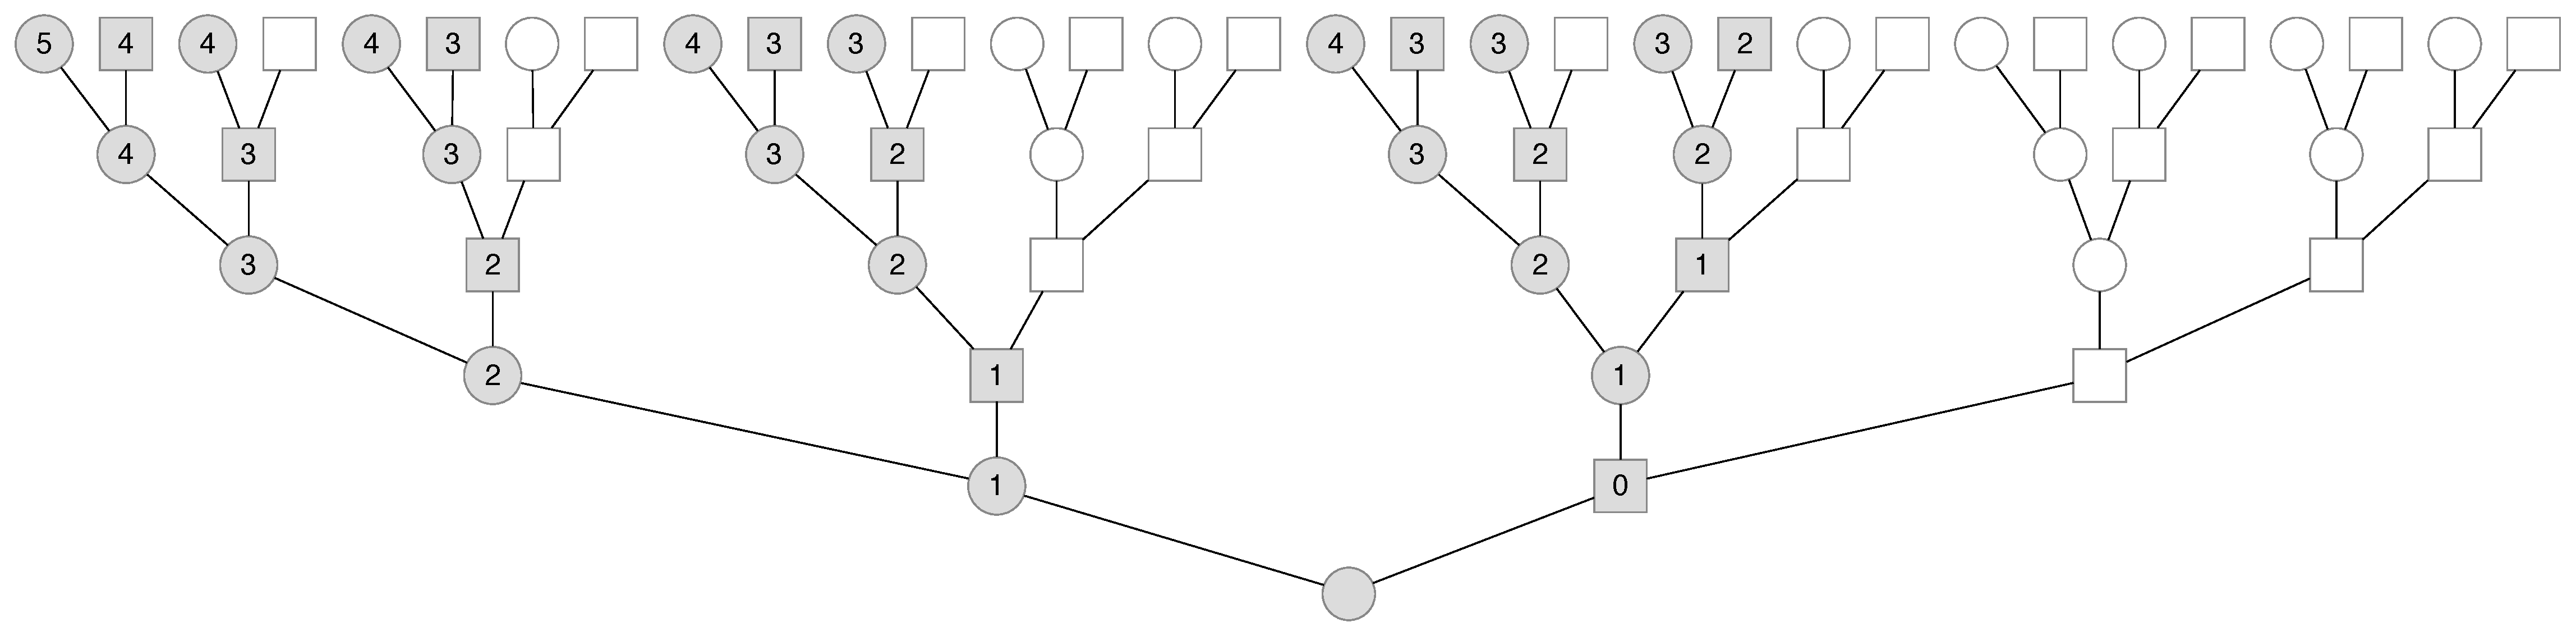
\includegraphics[width=\textwidth]{figures/chapter_1/x-rm-tree.eps}

  \caption[Genealogy with embedded X chromosome geneaology]{A genealogy back
    five generations with the embedded X genealogy.  Males are depicted as
    squares and females as circles.  Individuals in the X genealogy are shaded
    gray while unshaded individuals are ancestors that are not X ancestors.
  Each X ancestor is labeled with the number of recombinational meioses to the
present-day female.} \label{fig:x-rm-tree}

\end{figure*}

%% TODO
In Section \ref{sec:auto-ancestry} (and in Appendix \ref{ap:auto-cousin}) we
review models of autosomal identity by descent among relatives, on which we
base our models of X genetic ancestry.  Then, in Section \ref{sec:x-ancestry}
we look at X genealogies, as their properties affect the transmission of X
genetic material from X ancestors to a present-day individual. We develop
simple approximations to the probability distributions of the number and length
of X chromosome segments that will be shared IBD between a present-day female
and one of her X ancestors a known number of generations back. These models
provide a set of results for the X chromosome equivalent to those already known
for the autosomes \parencite{Donnelly:1983fi,thomas:1994hg}. Then, in Section
\ref{sec:shared-x-anc}, we look at shared X ancestry---when two present-day
cousins share an X ancestor a known number of generations back. We calculate
the probabilities that genealogical half- and full-cousins are also connected
through their X genealogy, and thus can potentially share genetic material on
their X. We then extend our models of IBD segment length and number to segments
shared between half- and full-cousins. Finally, in Section \ref{sec:inf} we
show that shared X genetic ancestry contains additional information (compared
to genetic autosomal ancestry) for inferring relationships among individuals,
and explore the limits of this information. 

\section{Autosomal Ancestry}
\label{sec:auto-ancestry}

To facilitate comparison with our X chromosome results, we first briefly review
analogous autosomal segment number and segment length distributions
\parencite{Donnelly:1983fi,thomas:1994hg,huff2011maximum}. Throughout this paper,
we assume that one's genealogical ancestors $k$ generations back are distinct
(e.g. there is no inbreeding), i.e. there is no pedigree collapse due to
inbreeding (see Appendix \ref{ap:ped-collapse} for a model of how this
assumption breaks down with increasing $k$). Thus, an individual has $2^k$
\emph{distinct} genealogical ancestors. Assuming no selection and fair meiosis,
a present-day individual's autosomal genetic material is spread across these
$2^k$ ancestors with equal probability, having been transmitted to the
present-day individual solely through recombination and segregation.

We model the process of crossing over during meiosis as a continuous time
Markov process along the chromosome, as in \textcite{thomas:1994hg} and
\textcite{huff2011maximum}, and described by \textcite{Donnelly:1983fi}. In
doing so we assume no crossover interference, such that in each generation $b$
recombinational breakpoints occur as a Poisson process running with a uniform
rate equal to the total length of the genetic map (in Morgans), $\nu$. Within a
single chromosome, $b$ breaks create a mosaic of $b+1$ alternating maternal and
paternal segments. This alternation between maternal and paternal haplotypes
creates long-run dependency between segments \parencite{liang2014lengths}.  We
ignore these dependencies in our analytic models by assuming that each
chromosomal segment survives segregation independently with probability
\nicefrac{1}{2} per generation. For $d$ independent meioses separating two
individuals, we imagine the Poisson recombination process running at rate $\nu
d$, and for a segment to be shared IBD between the two ancestors it must
survive $\nicefrac{1}{2^d}$ segregations.  Consequently, the expected number of
segments shared IBD between two individuals $d$ meioses apart in a genome with
$c$ chromosomes is approximated as \parencite{thomas:1994hg}:

\begin{align}
  \label{eq:exp-n}
  \E[N] &= \frac{1}{2^d} (\nu d + c)
\end{align}

Intuitively, we can understand the $\nicefrac{1}{2^d}$ factor as the
coefficient of kinship \parencite[or path
coefficient;][]{wright1922coefficients,wright1934method} of two individuals $d$
meioses apart, which gives the probability that two alleles are shared IBD
between these two individuals. Then, the expected number of IBD segments
$\E[N]$ can be thought of as the average number of alleles shared between two
individuals in a genome with $\nu d + c$ loci total. Under this approximation,
recombination increases the number of independent loci linearly each generation
(by a factor of the total genetic length). A fraction $\nicefrac{1}{2^d}$ of
parental alleles at these loci survive the $d$ meioses to be IBD with the
present-day individual.

By convention, we count the number of contiguous IBD segments $N$ in the
present-day individual, not the number of contiguous segments in the ancestor.
For example, an individual will share exactly one block per chromosome with
each parent if we count the contiguous segments in the offspring, even though
these segments may be spread across the parent's two homologues. This
convention, which we use throughout the paper, is identical to counting the
number of IBD segments that occur in $d-1$ meioses rather than $d$ meioses.
This convention only impacts models of segments shared IBD between an
individual and one of their ancestors; neither the distribution of segment
lengths nor the distributions for segment number shared IBD between cousins are
affected by this convention.

\subsection{The distribution of IBD segments between a present-day individual
and an ancestor} 
\label{sec:auto-dist-ibd-seg}

Given that a present-day individual and an ancestor in the $k^\text{th}$
generation are separated by $k$ meioses, the number of IBD segments can be
modeled with what we call the \emph{Poisson-Binomial} approximation. Over $d=k$
meioses, $B=b \sim \text{Pois}(\nu k)$ recombinational breakpoints fall on $c$
independently assorting chromosomes, creating $b + c$ segments. Ignoring
long-range dependencies, we assume all of these $b+c$ segments have an
independent chance of surviving the $k$ segregations to the present-day
individual, and thus the probability that $n$ segments survive given $b+c$
trials is Binomially distributed with probability $\nicefrac{1}{2^k}$.
Marginalizing over the unobserved number of recombinational breakpoints $b$,
and replacing $k$ with $k-1$ to following the convention described above:

\begin{align}
  P(N=n | k) = \sum_{b=0}^\infty &\text{Bin}(N=n \;|\; l=b+c,
p=\nicefrac{1}{2^{k-1}}) \nonumber \\ 
&\times \text{Pois}(B=b \;|\; \lambda=\nu (k-1)) 
\end{align}

The expected value of the Poisson-Binomial model is given by equation
\eqref{eq:exp-n} with $d=k-1$ and this model is similar to those of
\textcite{thomas:1994hg,Donnelly:1983fi}. We can further approximate this by
assuming that we have a Poisson total number of segments with mean $(c +
\nu(k-1))$ and these segments are shared with probability
$\nicefrac{1}{2^{k-1}}$ as in \textcite{huff2011maximum}. This gives us a
thinned Poisson distribution of shared segments:

\begin{align}
\label{eq:auto-segment-number}
  P(N = n | k, \nu, c) &= \text{Pois}(N = n | \lambda = (c + \nu (k-1))/2^{k-1}) \nonumber \\
                       &= \frac{((c + \nu (k-1))/2^{k-1})^n  e^{- (c + \nu (k-1))/{2^{k - 1}}}}{n!}
\end{align}

This thinned Poisson model also has an expectation given by equation
\eqref{eq:exp-n} but compared to the Poisson-Binomial model has a larger
variance than the true process. This overdispersion occurs because modeling the
number of segments created after $b$ breakpoints involves incorporating the
initial number of chromosomes into the Poisson rate. However, this initial
number of chromosomes is actually fixed, which the Poisson-Binomial model
captures but the Poisson thinning model does not (i.e. one generation back such
that $k=1$, the thinning model treats the number of segments shared IBD with
one's parents is $N \sim \text{Pois}(c)$ rather than $c$). See Appendix
\ref{ap:pois-thin} for a further comparison of these two models. A more formal
description of this approximation as a continuous-time Markov process is given
in \textcite{thomas:1994hg}. In Appendix \ref{ap:auto-cousin}, we describe
similar results for the number of autosomal segments shared between cousins and
the length distributions of autosomal segments.

We will use similar models as these in modeling the length and number of X
chromosome segments shared been relatives. However, the nature of X genealogies
(which we cover in the next section) requires we adjust these models.
Specifically, while one always has $k$ recombinational meioses between an
autosomal ancestor in the $k^\text{th}$ generation, the number of
recombinational meioses varies across the lineages to an X ancestor with the
number of females in a lineage, since X homologous recombination only occurs in
females (Figure \ref{fig:x-rm-tree}). This varying number of recombinational
meioses across lineages leads to a varying-rate Poisson recombination process,
with the rate depending on the specific lineage to the X ancestor. After we
take a closer look at X genealogies in the next section, we adapt the models
above to handle the varying-rate Poisson process needed to model IBD segments
in X genealogies.

\section{X Ancestry}
\label{sec:x-ancestry}

\subsection{Number of Genealogical X Ancestors}

  \begin{figure*}[!ht]
    \centering
    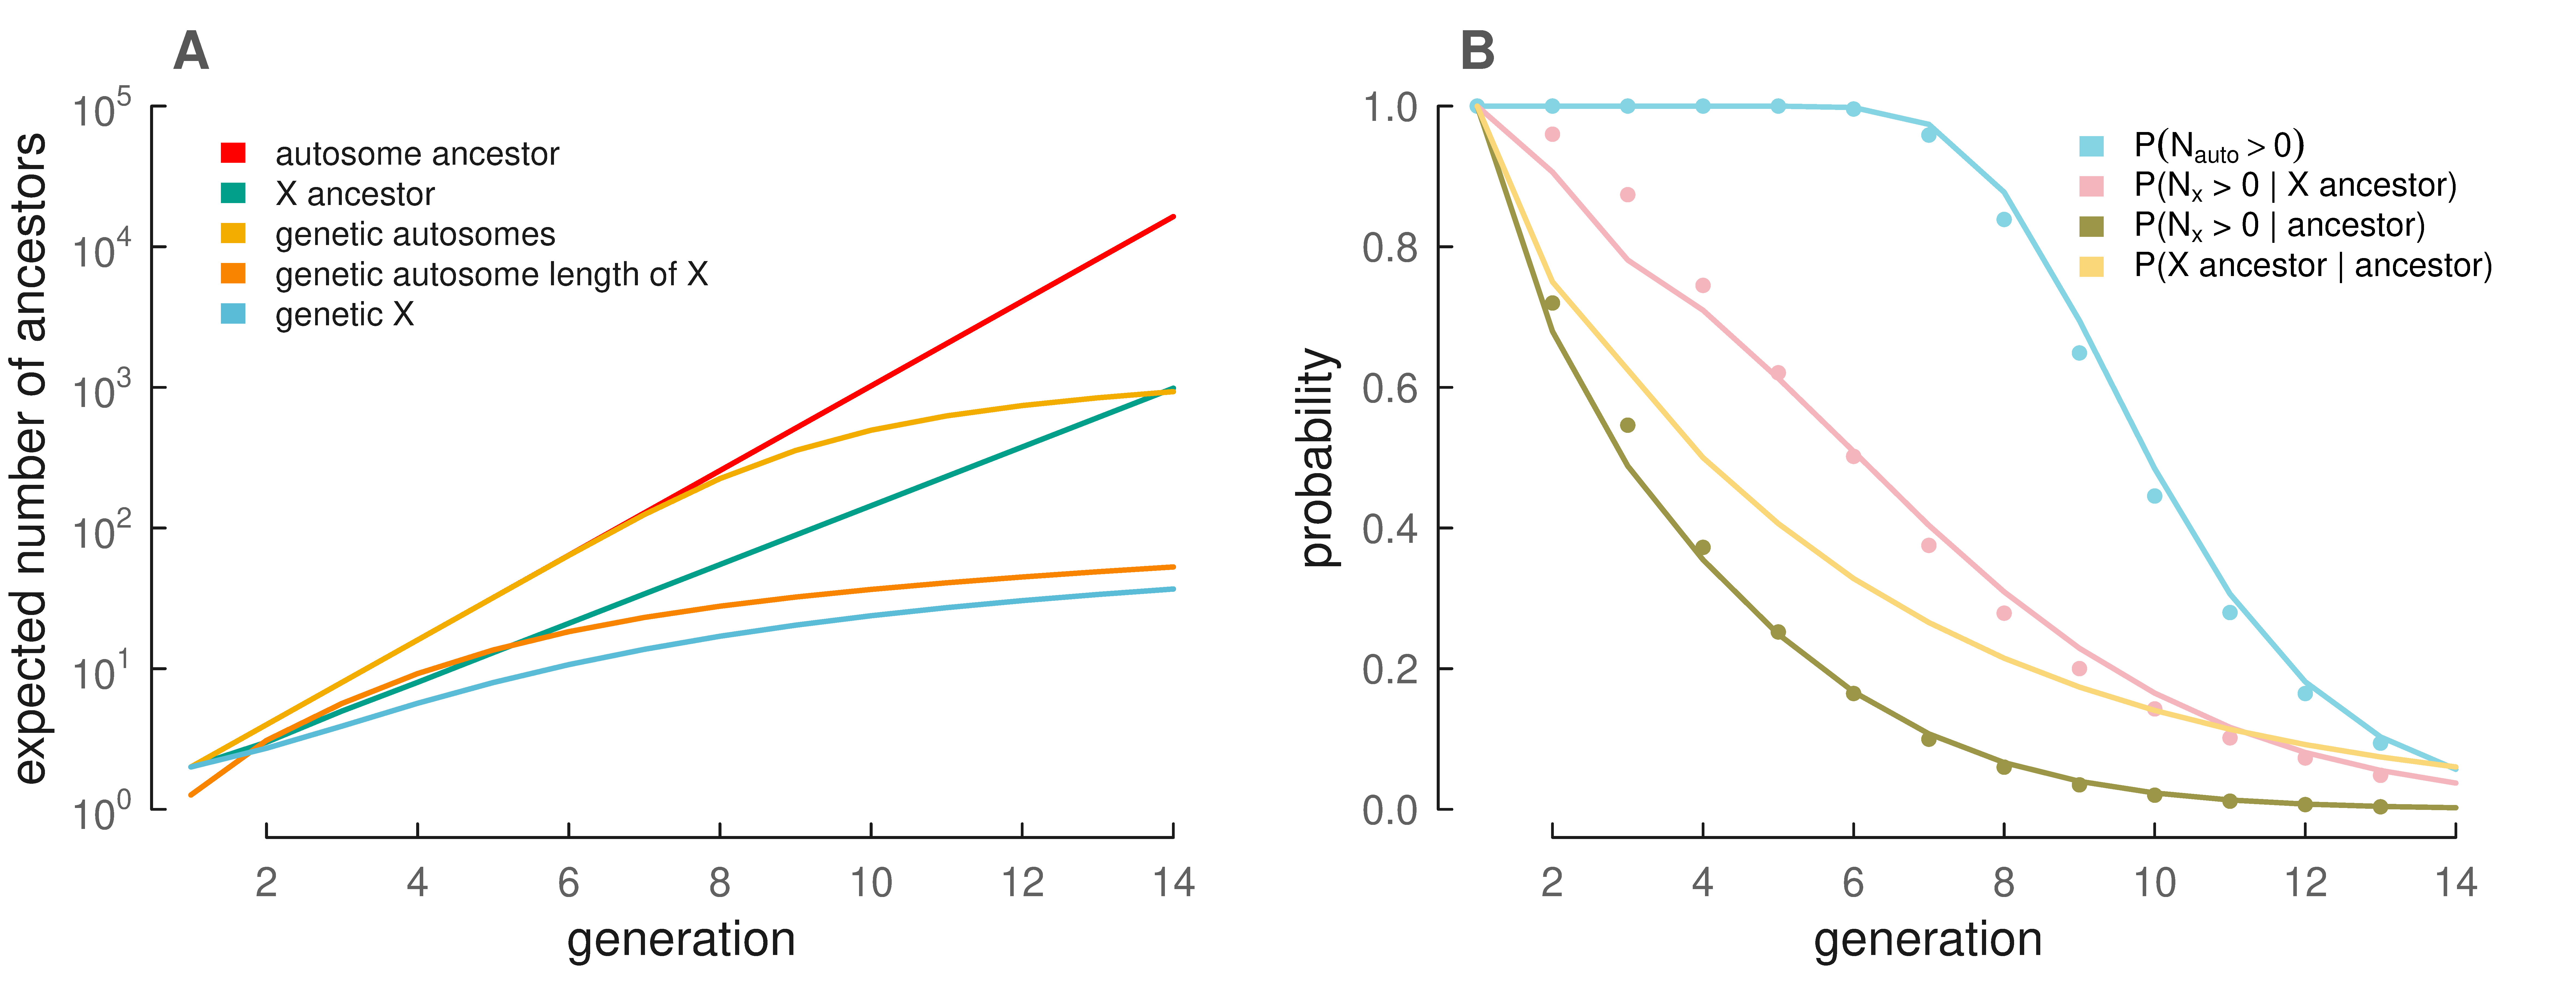
\includegraphics[width=0.9\textwidth]{figures/chapter_1/num-ancestors}

    \caption[Growth of genetic and genealogical ancestors, and probability of
    sharing genetic material]{How the number of genetic and genealogical
      ancestors and probabilities of sharing genetic material vary back through
      the generations for different cases. A: Each line represents a
      present-day female's expected number of ancestors (y-axis) in the
      $k^\text{th}$ generation (x-axis; where $k=1$ is parental generation),
      for a variety of cases. The present day female's number of genealogical
      ancestors in the $k^\text{th}$ generation is in red, and the expected
      number of these ancestors that contribute any autosome genetic material
      is in yellow.  Likewise, the present-day female's number genealogical X
      ancestors is in green, and the expected number of these ancestors that
      contribute any X genetic material is in blue. For comparison, the number
      of genetic ancestors of an autosome of length equal to the X is included
      (orange).  B: The probability of genealogical and genetic ancestry
      (y-axis) from an arbitrary ancestor in the $k^\text{th}$ generation
      (x-axis).  $P(\text{N}_\text{auto} > 0)$ is derived from equation
      \eqref{eq:auto-segment-number}, $P(\text{N}_\text{X} > 0 \;|\; \text{X
      ancestor})$ from equation \eqref{eq:x-number-block}, $P(\text{N}_\text{X}
      > 0 \;|\; \text{ancestor})$ from equations \eqref{eq:x-number-block} and
    \eqref{eq:prob-x-anc}, and $P(\text{X ancestor} \;|\; \text{ancestor})$
  from equation \eqref{eq:prob-x-anc}. Points show simulated results.}

\label{fig:num-ancestors}
\end{figure*}

While a present-day individual can potentially inherit autosomal segments from
any of its $2^k$ genealogical ancestors $k$ generations back, only a fraction
of these individuals can possibly share segments on the X chromosome. In
contrast to biparental genealogies, males have only one genealogical X
ancestor---their mothers---if we ignore the PAR. This constraint (which we
refer to throughout as the \emph{no two adjacent males condition}) shapes both
the number of X ancestors and the number of females along an X lineage. For
example, consider a present-day female's X ancestors one generation back: both
her father and mother contribute X chromosome material. Two generations back,
she has three X genealogical ancestors: her father only inherits an X from her
paternal grandmother, while her mother can inherit X material from either of
parents. Continuing this process, this individual has five X ancestors three
generations back and eight ancestors four generations back (Figure
\ref{fig:x-rm-tree}). 


In general, a present-day female's X genealogical ancestors is growing as a
Fibonacci series \parencite{laughlin1920calculating, Basin:1963wf}, such that $k$
generations back she has $\mathcal{F}_{k+2}$ X genealogical ancestors, where
$\mathcal{F}_k$ is the $k^\text{th}$ Fibonacci number (where $k$ is 0-indexed
and the series begins $F_0 = 0, F_1 = 1, \ldots$; Online Encyclopedia of
Integer Sequences reference \href{https://oeis.org/A000045}{A000045};
\citeauthor{sloane2014online}, \citeyear{sloane2014online}). We can demonstrate
that one's number of X genealogical ancestors ($n_k$) grows as a Fibonacci
series by encoding the X inheritance rules for the number of males and females
($m_k$ and $f_k$, respectively) in the $k^\text{th}$ generation as a set of
recurrence relations:

\begin{table}[htbp]
\centering
  \begin{tabularx}{\linewidth}{c c}
  $f_k = n_{k-1}$ & every individual receives an X chromosome from his/her mother \\
  $m_k = f_{k-1}$ & every female receives an X chromosome from her father \\
  $n_k = f_k + m_k$ & \\
\end{tabularx}
\end{table}

Rearranging these recurrence equations gives us $n_k = n_{k-1} + n_{k-2}$,
which is the Fibonacci recurrence. Starting with a female in the $k=0$
generation, we have initial values $n_0=1$ and $n_1 = 2$, which gives us the
Fibonacci numbers offset by two, $\mathcal{F}_{k+2}$. For a present-day male,
his number of X ancestors is $\mathcal{F}_{k+1}$, i.e. offset by one to count
the number of X ancestors his mother has. To simplify our expressions, we will
assume throughout the paper that all-present day individuals are female since a
simple offset can be made to handle males.

%\paragraph{Proportion of X ancestors} 

\begin{figure*}[!ht]
    \centering
    % change 0.49 to 0.5 for vertical alignment of subfigures
    \begin{subfigure}[b]{0.49\textwidth}
      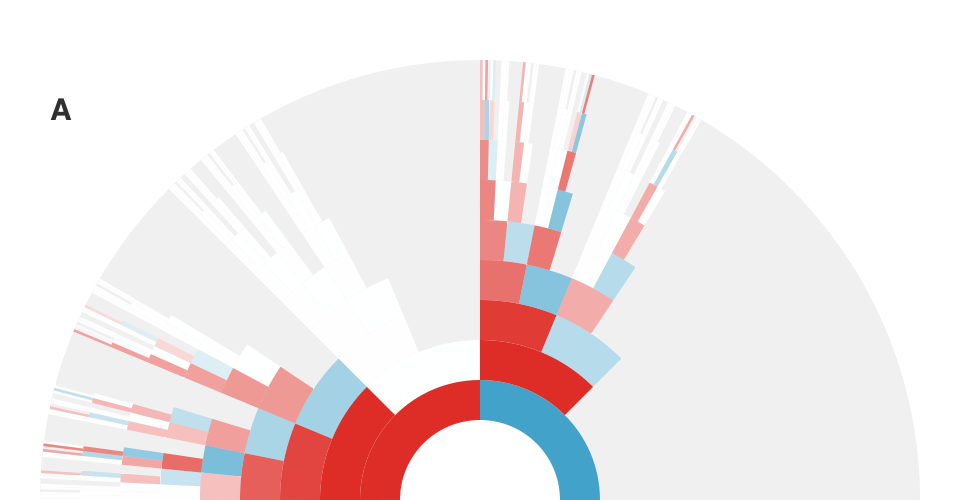
\includegraphics[width=\textwidth]{figures/chapter_1/x-arc}
    \end{subfigure}
    \begin{subfigure}[b]{0.49\textwidth}
      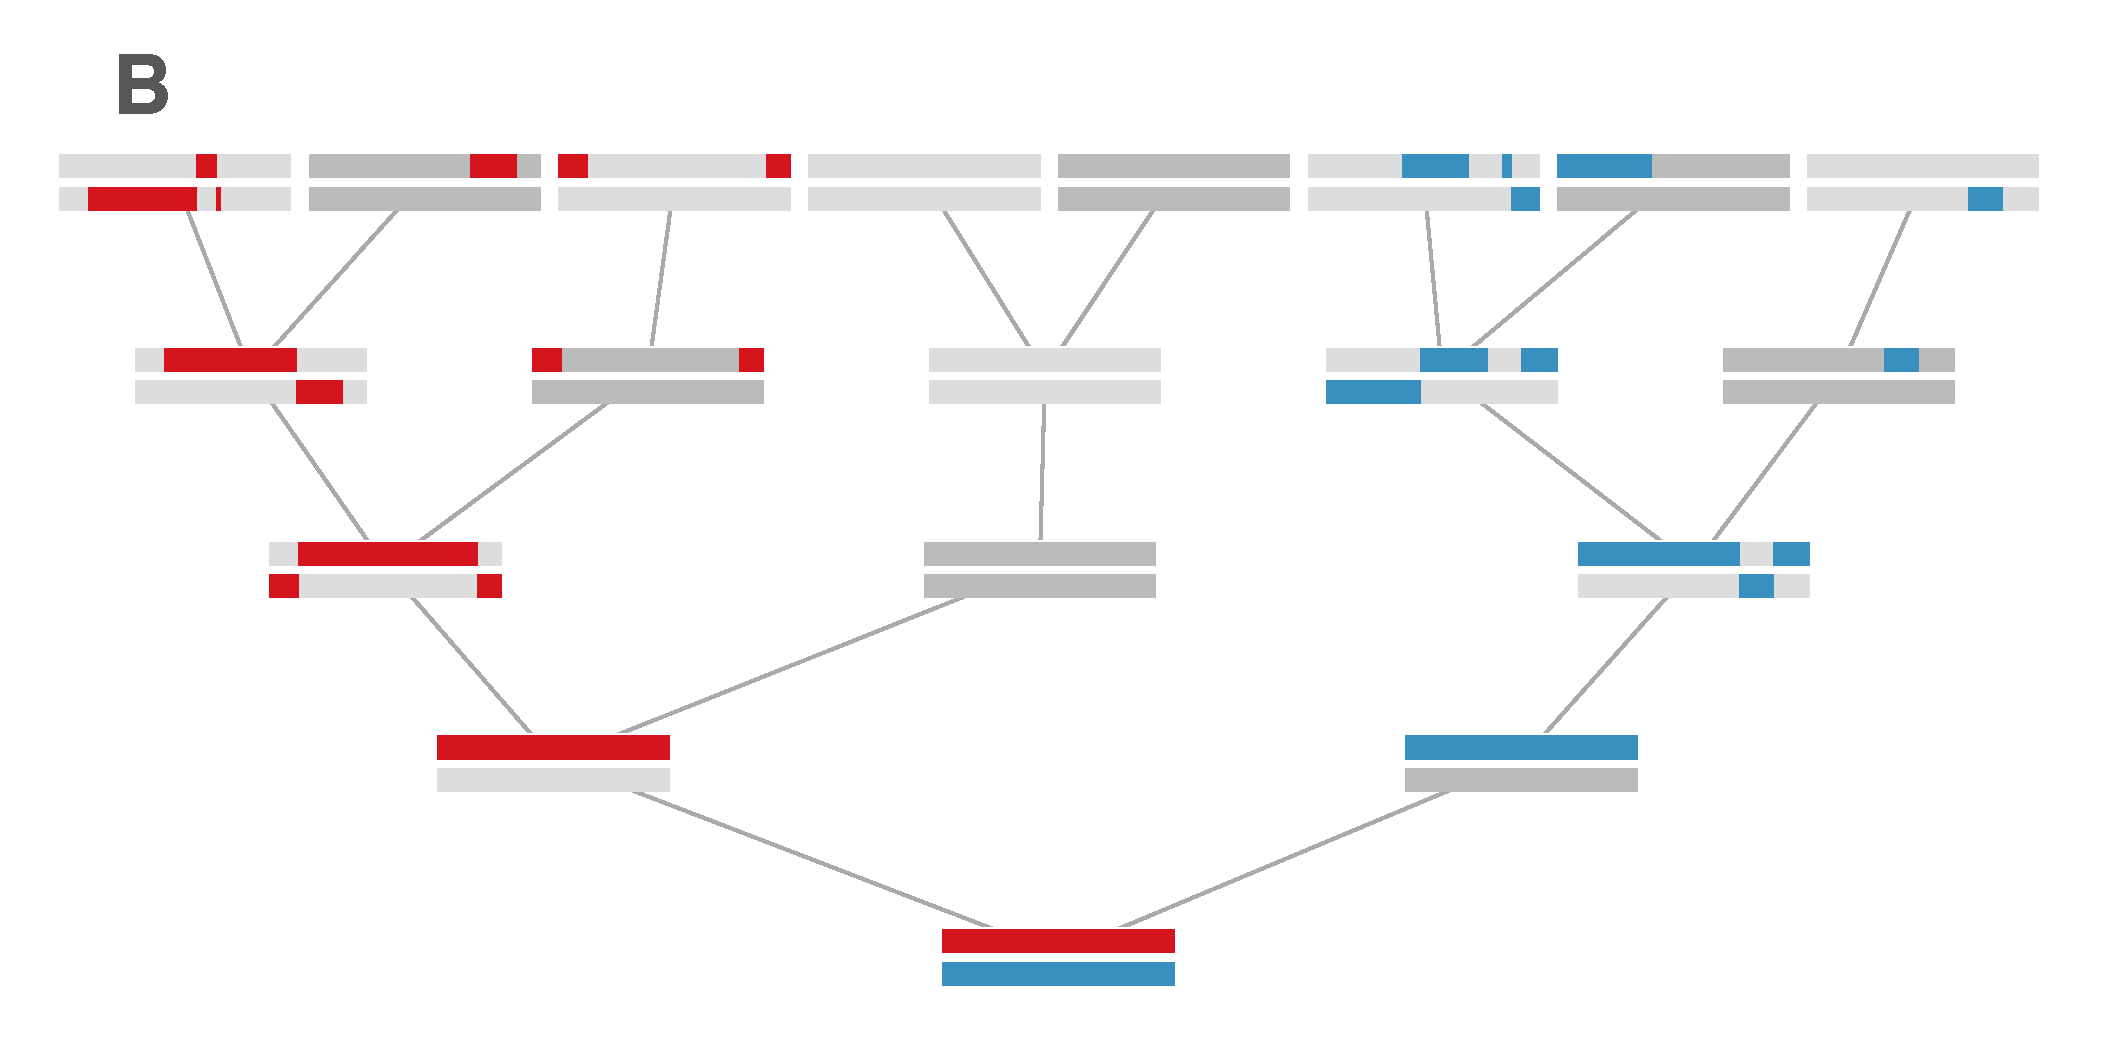
\includegraphics[width=\textwidth]{figures/chapter_1/x-tree}
    \end{subfigure}
    
    \caption[Graphical representation of X chromosome genealogy]{Graphical
      representations of an example X chromosome genealogy.  A: Simulated X
      genealogy of a present-day female, back nine generations.  Each arc is an
      ancestor, with female ancestors colored red, and male ancestors colored
      blue. The transparency of each arc reflects the genetic contribution of
      this ancestor to the present-day female.  White arcs correspond X
      genealogical ancestors that share no genetic material with the
      present-day female, and gray arcs are genealogical ancestors that are not
      X ancestors. B: The X segments of the simulation in (A), back five
      generations.  The maternal X lineage's segments are colored red, and the
    paternal X segments are colored blue. A male ancestor's sex chromosomes are
  colored dark gray (and include the Y) and a female ancestor's sex chromosomes
are colored light gray.}

    \label{fig:x-arc}

  \end{figure*}

In Figure \ref{fig:num-ancestors}A we show the increase in the number of X
genealogical and genetic ancestors (green and light blue) and compare these to
the growth of all of one's genealogical ancestors and autosomal genetic
ancestors. The closed-form solution for the $k^\text{th}$ Fibonacci number is
given by Binet's formula ($\mathcal{F}_n = ((1 + \sqrt{5})^n - (1 -
\sqrt{5})^n)/(2^n \sqrt{5})$), which shows that the Fibonacci sequence grows at
an exponential rate slower than $2^k$. 

Consequently, the fraction of ancestors who can contribute to the X chromosome
declines with $k$. Given that a female has $\mathcal{F}_{k+2}$ X ancestors and
$2^k$ genealogical distinct ancestors, her proportion of X ancestors is:

\begin{equation}
  \label{eq:prob-x-anc}
  P(\text{X ancestor} \;|\; \text{ancestor}) = \frac{\mathcal{F}_{k+2}}{2^k} 
\end{equation}
%
This fraction can also be interpreted as the probability that a randomly chosen
genealogical ancestor $k$ generations ago is also an X genealogical ancestor.
We show this probability as a function of generations into the past in Figure
\ref{fig:num-ancestors}B (yellow line).

From our recurrence equations we can see that a present-day female's
$\mathcal{F}_{k+2}$ ancestors in the $k^\text{th}$ generation are composed of
$\mathcal{F}_{k+1}$ females and $\mathcal{F}_{k}$ males. Likewise for a
present-day male, his $\mathcal{F}_{k+1}$ ancestors in the $k^\text{th}$
generation are composed of $\mathcal{F}_{k}$ females and $\mathcal{F}_{k-1}$
males. We will use these results when calculating the probability of a shared X
ancestor.

\subsection{Ancestry Simulations} 

In the next sections, we use stochastic simulations to verify the analytic
approximations we derive; here we briefly describe the simulation methods. We
have written a C and Python X genealogy simulation procedure (source code
available in File S1 and at \url{https://github.com/vsbuffalo/x-ancestry/}). We
simulate a female's X chromosome genetic ancestry back through her X genealogy.
Figure \ref{fig:x-arc} visualizes the X genetic ancestors of one simulated
example X genealogy back nine generations to illustrate this process. Each
simulation begins with two present-day female X chromosomes, one of which is
passed to her mother and one to her father. Segments transmitted to a male
ancestor are simply passed directly back to his mother (without recombination).
For segments passed to a female ancestor, we place a Poisson number of
recombination breakpoints (with mean $\nu$) on the X chromosome and the segment
is broken where it overlaps these recombination events. The first segment along
the chromosome is randomly drawn to have been inherited from either her
mother/father, and we alternate this choice for subsequent segments. This
procedure repeats until the target generation back $k$ is reached. The segments
in the $k$-generation ancestors are then summarized as either counts (number of
IBD segments per individual) or lengths.  These simulations are necessarily
approximate as they ignore crossover interference.  However, unlike our
analytic approximations, our simulation procedure maintains long-run
dependencies created during recombination, allowing us to see the extent to
which assuming independent segment survival adversely impacts our analytic
results.

\subsection{The number of recombinational meioses along an unknown X lineage}

If we pick an ancestor at random $k$ generations ago, the probability that they
are an X genealogical ancestor is given by equation \eqref{eq:prob-x-anc}. We
can now extend this logic and ask: having randomly sampled an X genealogical
ancestor, how many recombinational meioses (i.e. females) lie in the lineage
between a present day individual and this ancestor? Since IBD segment number
and length distributions are parameterized by a rate proportional to the number
of recombination events, this quantity is essential to our further derivations.
Specifically, if there's uncertainty about the particular lineage between a
present-day female and one of her X ancestors $k$ generations back (such that
all of the $\mathcal{F}_{k+2}$ lineages to an X ancestor are equally probable),
the number of females (thus, recombinational meioses) that occur is a random
variable $R$. By the no two adjacent males condition, the possible number of
females $R$ is constrained; $R$ has a lower bound of $\lfloor \nicefrac{k}{2}
\rfloor$, which corresponds to male-female alternation each generation to an
ancestor in the $k^\text{th}$ generation. Similarly, the upper bound of $R$ is
$k$, since it is possible every individual along one X lineage is a female.
Noting that an X genealogy extending back $k$ generations enumerates every
possible way to arrange $r$ females such that none of the $k-r$ males are
adjacent, we find that the number of ways of arranging $r$ such females this
way is

\begin{equation}
{ r + 1 \choose k - r}.
\end{equation}

For some readers, it may be useful to visualize the relationship between the
numbers of recombinational meioses across the generations using Pascal's
triangle (Figure \ref{fig:pascals-bifib}). The sequence of recombinational
meioses is related to a known integer sequence; see Online Encyclopedia of
Integer Sequences reference \href{https://oeis.org/A030528}{A030528}
\parencite{sloane2014online} for a description of this sequence and its other
applications.

If we pick an X genealogical ancestor at random $k$ generations ago the
probability that there are $r$ female meioses along the lineage leading to this
ancestor is
\begin{align}
  \label{eq:recomb-pmf}
  P_R(R = r | k) = \frac{{r + 1 \choose k - r}}{\mathcal{F}_{k+2}}.
\end{align}

In Appendix \ref{ap:generating-function}, we derive a generating function for
the number of recombinational meioses. We can use this generating function to
obtain properties of this distribution such as the expected number of
recombinational meioses. We can show that the expected number of
recombinational meioses converges rapidly to $\E[R] \approx
(\nicefrac{\varphi}{\sqrt{5}}) \; k$ with increasing $k$, where $\varphi$ is
the Golden Ratio, $\frac{1 + \sqrt{5}}{2}$.

\begin{figure}[!ht]
  \centering
  
\includegraphics[width=\linewidth]{figures/chapter_1/bifib}

  \caption[Visualization of the distribution of recombinational meioses]{The
    number of individuals (black numbers) with $r$ recombinational meioses
    (each diagonal, labeled at base of triangle) for a generation $k$ (each
    row). This encodes the number of recombinational meioses as the binomial
    coefficient ${r + 1 \choose k - r}$. Each value is further decomposed into
    the number of recombinational meioses from the female (red value, upper
    left) and male (blue value, upper right) lineages. Each black value is
    calculated by adding the black number to the left in the row above (the
    number of recombinational meioses from the maternal side) and the black
    number two rows directly above (the number of recombinational meioses from
    the paternal side). The sum of each row (fixed $k$) is a Fibonacci number
    and the values in the diagonal corresponding to a fixed value of $r$ are
    binomial coefficients. Reading from the top left side to bottom right
  corner, Pascal's triangle is contained in the red, blue, and black numbers.}

  \label{fig:pascals-bifib}

\end{figure}


\subsection{The Distribution of Number of Segments Shared with an X Ancestor}

Using the distribution of recombinational meioses derived in the last section,
we now derive a distribution for the number of IBD segments shared between a
present-day individual and an X ancestor in the $k^\text{th}$ generation. For
clarity, we first derive the number of IBD segments counted in the
\emph{parents} (i.e. not following the convention described in Section
\ref{sec:auto-ancestry}), but we can adjust this simply by replacing $k$ with
$k-1$.

First, we calculate the probability of a present-day individual sharing $N=n$
IBD segments with an X genealogical ancestor $k$ generations in the past, where
it is \emph{known} that there are $R=r$ females (and thus recombinational
meioses) along the lineage to this ancestor. This probability uses the
Poisson-Binomial model described in Section \ref{sec:auto-dist-ibd-seg}:
%
\begin{align}
  P(N=n | r, k, \nu) = \sum_{b=0}^\infty &\text{Bin}(N=n \;|\; l=b+1, p=\nicefrac{1}{2^r}) \nonumber \\
  &\times \text{Pois}(B=b \;|\; \lambda=\nu r)
  \label{eq:likelihood-n}
\end{align}
%

Note that once we have conditioned on the number of recombinational meioses $r$,
the lineages to an X ancestor are interchangeable; the specific X lineage
affects recombination (and thus the IBD number and length distributions) only
through the number of recombinational meioses along the lineage. 

If we consider an X genealogical ancestor $k$ generations back, this individual
could be any of the present-day female's $\mathcal{F}_{k+2}$ X ancestors. Since
the particular lineage to this ancestor is unknown, we marginalize over all
possible numbers of recombinational meioses that could occur:

\begin{figure*}[!ht]
  \centering
  
\includegraphics[width=\textwidth]{figures/chapter_1/x-ancestor-blockcounts}

  \caption[Comparison of the Poisson thinning approximation and Poisson-Binomial model]{The Poisson thinning (yellow lines) and Poisson-Binomial
    (blue lines) analytic distributions of IBD segment number between an X
    ancestor in the $k^\text{th}$ generation (each panel) and a present-day
    female. Simulation results averaged over 5,000 simulations are the gray
  points.}

  \label{fig:x-ancestor-blockcounts}

\end{figure*}

%% TODO 
\begin{alignat*}{2}
  &P(N=n | k, \nu)& \nonumber \\ 
  =& \sum_{r=\lfloor k/2 \rfloor}^k \sum_{b=0}^\infty &\text{Bin}(N=n | l=b+1, p=\nicefrac{1}{2^r}) \nonumber \\ 
  & &\times \; \text{Pois}(B=b \;|\; \lambda=\nu r) \; \frac{{r+1 \choose k-r}}{\mathcal{F}_{k+2}} \nonumber \\
  =& \sum_{r=\lfloor k/2 \rfloor}^k \sum_{b=0}^\infty &{b + 1 \choose n } \nicefrac{1}{2^{rn}}(1 - \nicefrac{1}{2^r})^{b - n + 1} \nonumber\\ 
  & & \times \; \frac{(\nu r)^b e^{-\nu r}}{b!} \; \frac{{r+1 \choose k-r}}{\mathcal{F}_{k+2}}
\end{alignat*}

For the distribution of number of IBD segments counted in the offspring, we
substitute $k-1$ for $k$

\begin{align}
  P(N=n \;|\; k, \nu) = \sum_{r=\lfloor (k-1)/2 \rfloor}^{k-1} \sum_{b=0}^\infty &\text{Bin}(n \;|\; l=b+1, p=\nicefrac{1}{2^r})  \nonumber \\& \times \text{Pois}(B=b \;|\; \lambda=\nu r) \; \nonumber \\ 
  & \times \frac{{r+1 \choose k-r-1}}{\mathcal{F}_{k+1}}.
  \label{eq:x-number-block}
\end{align}
%
In this formulation, if $k=1$, $r = 0$. In this case, the lack of
recombinational meioses implies $b=0$, such that a present-day female shares
$n=1$ X chromosomes with each of her two parents in the $k=1$ generation with
certainty. These segment number distributions are visualized in Figure
\ref{fig:x-ancestor-blockcounts} (light blue lines) alongside simulated results
(gray points).

We can use our equation \eqref{eq:x-number-block} to obtain $P(N > 0)$, the
probability that a genealogical X ancestor $k$ generations ago is a
\emph{genetic} ancestor. This probability over $k \in \{1, 2, \ldots, 14\}$
generations is shown in Figure \ref{fig:num-ancestors}B. For comparison, Figure
\ref{fig:num-ancestors}B also includes the probability of a genealogical
ancestor in the $k^\text{th}$ generation being an autosomal genetic ancestor
and the probability of being a genetic X ancestor unconditional on being an X
genealogical ancestor. 

We have also assessed the Poisson thinning approach to modeling X IBD segment
number. As with the Poisson-Binomial model, we marginalize over $R$:

\begin{align}
  P(N=n \;|\; k, \nu) = \sum_{r=r_{M}}^{k-1} 
  & \text{Pois}(B=b \;|\; \lambda=(1 + \nu r)/2^r) 
 \nonumber \\  &\times \frac{{r+1 \choose k-r-1}}{\mathcal{F}_{k+1}}
  \label{eq:x-number-block-thinned}
\end{align}

where $r_{M} = \lfloor (k-1)/2 \rfloor$.

In Figure \ref{fig:x-ancestor-blockcounts} we have compared the
Poisson-Binomial and Poisson-thinning approximations for the number of IBD
segments (counted in the offspring) shared between an X-ancestor in the
$k^\text{th}$ generation and a present-day female. Overall, the analytic
approximations are close to the simulation results, with the Poisson-Binomial
model a closer approximation for small $k$ and both models' accuracy improving
quickly with increasing $k$.  For a single chromosome (like the X), the
Poisson-thinning model offers a noticeable worse fit than it does for the
autosomes due to overdispersion discussed in Section
\ref{sec:auto-dist-ibd-seg} (see Appendix \ref{ap:pois-thin} for details).
Throughout the paper, we use the more accurate Poisson-Binomial model rather
than this Poisson thinning model. If only X ancestry more than 3 generations
back is of interest, the Poisson thinning approach may be used without much
loss of accuracy.


\subsection{The Distribution of IBD Segment Lengths with an X Ancestor}

The distribution of IBD segment lengths between a present-day female and an
unknown X genealogical ancestor in the $k^\text{th}$ generation is similar to
the autosomal length distribution described in Appendix \ref{ap:auto-cousin}
(equation \ref{eq:auto-seg-lens}). However, with uncertainty about the
particular lineage to the X ancestor, the number of recombinational meioses can
vary between $\lfloor \nicefrac{k}{2} \rfloor \le r \le k$; we marginalize over
the unknown number of recombinational meioses using the distribution equation
\eqref{eq:recomb-pmf}. Our length density function is:

\begin{equation}
  \label{eq:x-anc-length}
  p(U = u | k) = \sum_{r=\lfloor k/2 \rfloor}^k  r e^{-ru} \frac{{r+1 \choose k-r}}{\mathcal{F}_{k+2}} 
\end{equation}

In Figure \ref{fig:x-len-dist}, we compare our analytic length density to an
empirical density of X segment lengths calculated from 5,000 simulations. As
with our IBD segment number distributions, our analytic model is close to the
simulated data's empirical density, and converges rapidly with increasing $k$.

\begin{figure*}[!ht]
  \centering
  
\includegraphics[width=\textwidth]{figures/chapter_1/x-ancestor-blocklens}

  \caption[Analytic and simulated distributions of the X IBD segment length]{The
    analytic distributions of IBD segment length between an ancestor in the
    $k^\text{th}$ generation (for $k \in \{2, \ldots, 7\}$) and a present-day
    female (blue lines), and the binned average over 5,000 simulations (gray
  points).}

  \label{fig:x-len-dist}
\end{figure*}

Note that both the IBD segment length and number distributions marginalize over
an unobserved number of recombinational meioses ($R$) that occur along the
lineage between individuals. As the IBD segments shared between two individuals
is a function of the number breakpoints $B$, and thus recombinational meioses,
the length and number distributions $P(N = n)$ and $p(U = u)$ (which separately
marginalize over both $R$ and $B$) are not independent of one another.

\section{Shared X Ancestry}
\label{sec:shared-x-anc}

Because only a fraction of one's genealogical ancestors are X ancestors (and
this fraction rapidly decreases with $k$; see equation \eqref{eq:prob-x-anc}),
two individuals sharing X segments IBD from a recent ancestor considerably
narrows the possible ancestors they could share. In this section, we describe
the probability that a genealogical ancestor is an X ancestor, and the
distributions for IBD segment number and length across full- and half-cousin
relationships. For simplicity we concentrate on the case where the cousins
share a genealogical ancestor $k$ generations ago in both of their pedigrees,
i.e. the individuals are $k-1$ degree cousins. The formulae could be
generalized to ancestors of unequal generational-depths (e.g. second cousins
once removed) but we do not pursue this here.

\subsection{Probability of a Shared X Ancestor} 

Two individuals share their first common genealogical ancestor in the
$k^\text{th}$ generation if one of an individual's $2^k$ ancestors is also one
of the other individual's ancestors $k$ generations back. Given this shared
ancestor, we can calculate the probability that this single ancestor is also an
X genealogical ancestor. Since this shared ancestor must be of the same sex in
each of the two present-day individuals' genealogies, we condition on the
ancestor's sex (with probability $\nicefrac{1}{2}$ each) and then calculate the
probability that this individual is also an X ancestor (with the same sex). Let
us define $N_{\venus}$ and $N_{\mars}$ as the number of genealogical female and
male ancestors, and $N_{\venus}^X$ and $N_{\mars}^X$ as the number of X female
and male ancestors of a present-day individual in the $k^\text{th}$ generation.
Then:

\begin{align}
  P(\text{shared X ancestor} & \; | \; \text{shared ancestor } k \text{ generations})  \nonumber\\
  &= \frac{N_{\venus}}{2^k}\left(\frac{N_{\venus}^X}{N_{\venus}}\right)^2 + 
  \frac{N_{\mars}}{2^k}\left(\frac{N_{\mars}^X}{N_{\mars}}\right)^2 \nonumber \\
  &= \frac{1}{2}\left(\frac{\mathcal{F}_{k+1}}{2^{k-1}}\right)^2 + \frac{1}{2}\left(\frac{\mathcal{F}_k}{2^{k-1}}\right)^2
  \label{eq:prob-shared-x-ancestor}
\end{align}

Thus, the probability that a shared genealogical ancestor is also a shared X
ancestor is decreasing at an exponential rate. By the $8^\text{th}$ generation,
a shared genealogical ancestor has less than a five percent chance of being a
shared X ancestor of both present-day individuals.

\subsection{The Sex of Shared Ancestor}
\label{p:sex-of-shared-ancestor}

Unlike genealogical ancestors---which are equally composed of males and
females---recent X genealogical ancestors are predominantly female. Since a
present-day female has $\mathcal{F}_{k+1}$ female ancestors and
$\mathcal{F}_{k}$ male ancestors $k$ generations ago, the ratio of female to
male X genealogical ancestors converges to the Golden Ratio $\varphi = \frac{1
+ \sqrt{5}}{2}$ \parencite{simson1753explication}.

\begin{equation}
  \lim_{k \to \infty} \frac{\mathcal{F}_{k+1}}{\mathcal{F}_k} = \varphi
\end{equation}

In modeling the IBD segment number and length distributions between present day
individuals, the sex of the shared ancestor $k$ generations ago affects the
genetic ancestry process in two ways. First, a female shared ancestor allows
the two present-day individuals to share segments on either of her two X
chromosomes while descendents of a male shared ancestor share IBD segments only
through his single X chromosome. Second, the no two adjacent males condition
implies a male shared X genealogical ancestor constrains the X genealogy such
that the present-day X descendents are related through his two daughters.
Given that the ratio of female to male X ancestors is skewed, our later
distributions require an expression for the probability that a shared X
ancestor in the $k^\text{th}$ generation is female, which we work through in
this section.

As in equation \eqref{eq:prob-shared-x-ancestor}, an ancestor shared in the
$k^\text{th}$ generation of two present-day individuals' genealogies must have
the same sex in each genealogy. Assuming both present-day cousins are females,
in each genealogy there are $\mathcal{F}_k$ possible male ancestors and
$\mathcal{F}_{k+1}$ female ancestors that could be shared. Across each
present-day females' genealogies there are $(\mathcal{F}_k)^2$ possible male
ancestor combinations and $(\mathcal{F}_{k+1})^2$ possible female ancestor
combinations. Thus, if we let $\fsxa$ and $\msxa$ denote that the sex of the
shared is female and male respectively, the probability of a female shared
ancestor is: 

\begin{equation}
  P(\fsxa) = \frac{(\mathcal{F}_{k+1})^2}{(\mathcal{F}_k)^2 + (\mathcal{F}_{k+1})^2}
\end{equation}

The probability that the shared ancestor is male is simply $1-P(\fsxa)$. One
curiosity is that as $k \to \infty$, $P(\fsxa) \to \frac{\varphi}{\sqrt{5}} =
\frac{5 + \sqrt{5}}{10} \approx 0.7236$, where $\varphi$ is the Golden Ratio.

\subsection{Partnered Shared Ancestors}

Thus far, we have only looked at two present-day individuals sharing a single X
ancestor $k$ generations back. In monogamous populations, most shared ancestry
is likely to descend from \emph{two} ancestors; we call such relationships
\emph{partnered} shared ancestors. In this section, we look at full-cousins
descending from two shared genealogical ancestors that may also be X ancestors.
Two full-cousins could either (1) both descend from two X ancestors such that
they are X full-cousins, (2) share only one X ancestor, such that they are X
half-cousins, or (3) share no X ancestry. We calculate the probabilities
associated with each of these events here.

Two individuals are full-cousins if the $\text{great}^{k-2}$ grandfather and
the $\text{great}^{k-2}$ grandmother in one individual's genealogy are in the
other individual's genealogy. For these two full-cousins to be X full-cousins,
this couple must also be a couple in both individuals' X genealogies. In every
X genealogy, the number of couples in generation $k$ is the number of females
in generation $k-1$, as every female has two X ancestors in the prior
generation (while males only have one). Thus, the probability two female $k-1$
degree full-cousins are also X full-cousins is:

\begin{equation}
  P(\text{X full-cousins} \; | \; \text{full-cousins}) = 
    \left( \frac{\mathcal{F}_k}{2^{k-1}} \right)^2
\end{equation}


Now, we consider the event that two genealogical full-cousins are X
half-cousins. Being X half-cousins implies that the partnered couple these
full-cousins descend from includes a single ancestor that is in the X
genealogies of both full-cousins. This single X ancestor must be a female, as a
male X ancestor's female partner must also be an X ancestor (since mothers must
pass an X). For a female to be an X ancestor but not her partner, one or both
of her offspring must be male. Either of these events occurs with probability:

\begin{equation}
  P(\text{X half-cousins} \;|\; \text{full-cousins}) = \frac{\mathcal{F}_{k-1}^2 + 2 \mathcal{F}_{k-1} \mathcal{F}_k}{2^{2(k-1)}}
\end{equation}

\subsection{The Distribution of Recombinational Meioses between Two X Half-Cousins}
\label{p:two-cousins-rms}

To find distributions for the number and lengths of IBD segments shared between
two half-cousins on the X chromosome, we first need to find the distribution
for the number of females between two half-cousins with a shared ancestor in
the $k^\text{th}$ generation. We refer to the individuals connecting the two
cousins as a \emph{genealogical chain}. As we'll see in the next section, the
number of IBD X segments shared between half-cousins depends on the sex of the
shared ancestor; thus, we also derive distributions in this section for the
number of recombinational meioses along a genealogical chain, conditioning on
the sex of the shared ancestor. As earlier, our models assume two present-day
female cousins but are easily extended to male cousins.

First, there are $2k-1$ ancestral individuals separating two present-day female
$(k-1)^\text{th}$ degree cousins. These X ancestors in the genealogical chain
connecting the two present-day female cousins follow the no two adjacent male
condition; thus the distribution of females follows the approach used in
equation \eqref{eq:recomb-pmf} with $k$ replaced with $2k-1$:

\begin{equation}
  \label{eq:recomb-sanc-pmf} P_{H}(R=r | k) = \frac{ {r+1 \choose 2k-r-1} }{\mathcal{F}_{2k+1}}
\end{equation}
%
where the $H$ (for half-cousin) subscript differentiates this equation from
equation \eqref{eq:recomb-pmf}, $k$ is the generation of the shared ancestor.
Similarly to equation \eqref{eq:recomb-pmf}, $r$ is bounded such that
$r_{H,M} \le r \le 2k - 1$, where $r_{H,M} = \lfloor (2k-1)/2
\rfloor$.


Now, we derive the probability of $R=r$ females conditional on the shared
ancestor being female, $\fsxa$. This conditional distribution differs from
equation \eqref{eq:recomb-sanc-pmf} since it eliminates all genealogical chains
with a male shared ancestor. We find the distribution of recombinational
meioses conditional on a female shared ancestor by placing the other $R'=r'$
females (the prime denotes we do not count the shared female ancestor here)
along the two lineages of $k-1$ individuals from the shared female ancestor
down to the present-day female cousins. These $R'=r'$ females can be placed in
both lineages by positioning $s$ females in the first lineage and $r'-s$
females in the second lineage, where $s$ follows the constraint $\lfloor
(k-1)/2 \rfloor \le s \le k-1$.  Our equation \eqref{eq:recomb-pmf} models the
probability of an X genealogical chain having $r$ females in $k$ generations;
here, we use this distribution to find the probabilities of $s$ females in
$k-1$ generations in one lineage and $r'-s$ females in $k-1$ generations in the
other lineage. As the number of females in each lineage is independent, we take
the product of these probabilities and sum over all possible $s$; this is the
discrete convolution of the number of females in two lineages $k-1$ generations
long.  Finally, we account for the shared female ancestor, by the transform $R
= R' + 1 = r$:

\begin{equation}
  \label{eq:prob-r-given-female}
  P_{H}(R=r | \fsxa, k) = \sum_{s=\lfloor (k-1)/2 \rfloor}^{k-1} \frac{ {s + 1 \choose k - s - 1 } { r - s \choose k + s - r } }{(\mathcal{F}_{k+1})^2}
\end{equation}

In general, this convolution approach allows us to find the distribution of
females in a genealogical chain under various constraints, and can easily be
extended to the case of a shared male X ancestor (with necessarily two
daughters).
 
Finally, note that we have modeled the number of \emph{females} in a
genealogical chain of $2k-1$ individuals. Thus far in our models, the number of
females has equaled the number of recombinational meioses. However, when
considering the number of recombinational meioses between half-cousins,
\emph{two} recombinational meioses occur if the shared ancestor is a female (as
she produced two independent gametes she transmits to her two offspring). Thus,
for a single shared X ancestor, the number of recombinational meioses $\rho$ is
%
\begin{equation}
  \rho = \begin{cases}
        r + 1 & \text{if} \; \fsxa\\
        r & \text{if} \; \msxa\\
      \end{cases}
\label{eq:recomb-total}
\end{equation}
%
which we use when parameterizing the rate of recombination in our IBD segment
number distributions. Furthermore, since a shared female ancestor has two X
haplotypes that present-day cousins could share segments IBD through, the
binomial probability $\nicefrac{1}{2^\rho}$ is doubled. Further constraints are
needed to handle full-cousins; we will discuss these below.

\subsection{Half-Cousins}
\label{p:ibd-seg-num-x}

In this section we calculate the distribution of IBD X segments shared between
two present-day female X half-cousins with a shared ancestor in the $k^\text{th}$
generation. We imagine we do not know any details about the lineages to this
shared ancestor nor the sex of the shared ancestor, so we marginalize over
both. Thus, the probability of two $(k-1)^\text{th}$ degree X half-cousins
sharing $N=n$ segments is:

\begin{align}
  \label{eq:prob-n-half-cousins}
  P(N=n | k)  = \sum_{r=r_{H,M}}^{2k-1} &P_{H}(R=r | k)  \nonumber \\
  &\times \left[  P(N = n | \fsxa, R=r) P(\fsxa | R=r) \; + \right. \nonumber \\
  &\times \left. P(N = n | \msxa, R=r) P(\msxa | R=r) \right]
\end{align}

As discussed in the previous section, the total number of recombinational
meioses along the genealogical chain between half-cousins depends on the
unobserved sex of the shared ancestor (i.e. equation \eqref{eq:recomb-total}).
Likewise, the binomial probability also depends on the shared ancestor's sex.
Accounting for these adjustments, the probabilities $P(N = n | \fsxa, R=r)$ and
$P(N = n | \msxa, R=r)$ are:

\begin{subequations}
\begin{align}
  P(N = n | \fsxa, R=r) = \sum_{b=0}^\infty  &\text{Pois}(B = b | \lambda = (r+1)\nu)  \nonumber \\
  &\times \text{Bin}(N=n | l = b + 1, p=\nicefrac{1}{2^r}) \label{eq:prob-n-each-female} \\
  P(N = n | \msxa, R=r) = \sum_{b=0}^\infty  &\text{Pois}(B = b | \lambda = r\nu)  \nonumber \\
  &\times \text{Bin}(N=n | l = b + 1, p=\nicefrac{1}{2^r}) \label{eq:prob-n-each-male} 
\end{align}
\end{subequations}

Since the sex of the shared ancestor depends on the number of females in the
genealogical chain between the two cousins (e.g. if $r=2k-1$, the shared
ancestor is a female with certainty), we require an expression for the
probability of the shared ancestor being male or female given $R=r$. Using
Bayes' theorem, we can invert the conditional probability $P(R = r | \fsxa)$ to
find that the probability that a shared X ancestor is female conditioned on $R$
females in the genealogical chain is

\begin{align}
  \label{eq:prob-female-given-r}
  P_{H}(\fsxa | R=r, k) =& \frac{\mathcal{F}_{2k-1} }{ { r+1 \choose 2k-r-1 }  \left( (\mathcal{F}_{k+1})^2 + (\mathcal{F}_k)^2 \right) }  \nonumber\\
  & \times \sum_{s=\lfloor (k-1)/2 \rfloor}^{k-1}  {s + 1 \choose k - s + 1 } { r - s \choose k + s - r }
\end{align}
%
and $P(\msxa | R=r)$ can be found as the complement of this probability.

\begin{figure*}[!ht]
  \centering

  
\includegraphics[width=\textwidth]{figures/chapter_1/x-full-half-blockcounts}

  \caption[Analytic and simulated distributions of the X IBD segment
  number]{Distributions of X IBD segment number for X half- (blue) and X
    full-cousins (yellow). Lines show the analytic approximations (equations
    \eqref{eq:prob-n-half-cousins} and \eqref{eq:prob-n-full-sibs}) and blue
    and yellow points show the probabilities for X half- and X full-cousins
  averaged over 5,000 simulations.}

  \label{fig:half-cousin-segment-number}
\end{figure*}

Inserting equations \eqref{eq:prob-n-each-female}, \eqref{eq:prob-n-each-male},
and \eqref{eq:prob-female-given-r} into \eqref{eq:prob-n-half-cousins} gives us
an expression for the distribution of IBD segment numbers between two
half-cousins with a shared ancestor $k$ generations ago. Figure
\ref{fig:half-cousin-segment-number} compares the analytic model in equation
\eqref{eq:prob-n-half-cousins} with the IBD segments shared between
half-cousins over 5,000 simulated pairs of X genealogies.

The density function for IBD segment lengths between X cousins (either half- or
full-cousins; length distributions are only affected by the number of
recombinations in the genealogical chain) is equation \eqref{eq:x-anc-length}
but marginalized over the number of recombinational meioses between two cousins
(equation \eqref{eq:recomb-sanc-pmf}) rather than the number of recombinational
meioses between a present-day individual and a shared ancestor. Simulations
show the length density closely matches simulation results (see Figure
\ref{fig:half-cousin-x-length} in the appendix).

\subsection{Full-Cousins}
\label{sec:full-cousins}

Full-cousin relationships allow descendents to share IBD autosomal segments
from either their shared maternal ancestor, shared paternal ancestral, or both.
In contrast, since males only pass an X chromosome to daughters, only
full-sibling relationships in which both offspring are female (due to the no to
adjacent males condition) are capable of leaving X genealogical descendents. We
derive a distribution for the number of IBD segments shared between
$(k-1)^\text{th}$ degree full X cousins by conditioning on this familial
relationship and marginalizing over the unobserved number of females from the
two full-sibling daughters to the present-day female full-cousins.

First, we find the number of females (including the two full-sibling daughters
in the $(k-1)^\text{th}$ generation) in the genealogical chain between the two
X full-cousins (omitting the shared male and female ancestors, which we account
for separately). Like equation \eqref{eq:prob-r-given-female}, this is a
discrete convolution:

\begin{equation}
  P_{F}(R = r, k) = \sum_{s = \lfloor (k-2)/2 \rfloor}^{k-2} \frac{{s+1 \choose k-s-2 } {r-s-1 \choose k-r+s}}{(\mathcal{F}_k)^2}
\end{equation}
%
where the $F$ subscript indicates this equation is for full-cousins.
This probability is valid for $r_{F,M} + 2 \le r \le 2k-2$ and
is 0 elsewhere, where $r_{F,M} = 2\lfloor (k-2)/2\rfloor + 2$. For
$N=n$ segments to be shared between two X full-cousins, $z$ segments can be
shared via the maternal shared X ancestor (where $0 \le z \le n$) and $n-z$
segments can be shared through the paternal shared X ancestor. We marginalize
over all possible values of $z$, giving us another discrete convolution:

\begin{align}
  \label{eq:prob-n-full-sibs}
  P(N = n | R=r) = \sum_{r=r_{F,M}}^{2k-2} \sum_{z=0}^{n} & P(N = z | \fsxa)  \nonumber\\
  & \times P(N = n - z | \msxa) P_{F}(R=r)
\end{align}
%
where
%
\begin{align}
  P(N = n | \fsxa, R=r) = \sum_{b=0}^\infty & \text{Bin}(N=n | l = b+1, p=\nicefrac{1}{2^{r+1}})  \nonumber\\
  &\times \text{Pois}(B=b | \lambda = \nu (r+2)) \\
  P(N = n | \msxa, R=r) = \sum_{b=0}^\infty & \text{Bin}(N=n | l = b+1, p=\nicefrac{1}{2^r})  \nonumber \\
  &\times \text{Pois}(B=b | \lambda = \nu r) 
\end{align}
%
are the probabilities of sharing $n$ segments through the shared female and
male X ancestors respectively. For the female shared ancestor, we account for
two additional recombinational meioses (one for each of the two gametes she
passes to her two daughters), and the fact she can share segments through
either of her X chromosomes (hence, why the binomial probability is
$\nicefrac{1}{2^{r+1}}$). We compare our analytic X full-cousin IBD segment
number results to 5,000 genealogical simulations in Figure
\ref{fig:half-cousin-segment-number}.

\section{Inference}
\label{sec:inf}

With our IBD X segment distributions, we now turn to how these can be used to
infer details about recent X ancestry. In practice, inferring the number of
generations back to a common ancestor ($k$) is best accomplished through the
signature of recent ancestry from the 22 autosomes, rather than through the
short X chromosome. A number of methods are available for the task of
estimating $k$ through autosomal IBD segments
\parencite{huff2011maximum,Henn:2012ij,Durand010512}.  Therefore, we concentrate on
questions about the extra information that the X provides conditional on $k$
being known with certainty. 

Here, we focus on two separate questions: (1) what is the probability of being
an X genealogical ancestor given that no IBD segments are observed, and (2) can
we infer details about the X genealogical chain between two half-cousins?
These questions address how informative the number of segments shared between
cousins is about the precise relationship of cousins. We assume that segments
of X chromosome IBD come only from the $k^{th}$ generation, and not from deeper
relationships or from false positives. In practice, inference from the X IBD
segments would have to incorporate both of these complications, and as such our
results represent best case scenarios.

\begin{figure}[!ht]
  \centering
  
\includegraphics[width=\linewidth]{figures/chapter_1/prob-xanc-n0.eps}

  \caption[Probability of X ancestry given no shared X genetic material]{The
    probability of X ancestry given no shared X genetic material.  Yellow solid
    line: the probability an individual in the $k^\text{th}$ generation
    (x-axis) is an X ancestor to a present-day female, given they share no X
    genetic material with her. Blue solid line: the probability that two
    half-cousins share an X ancestor in the $k^\text{th}$ generation, given
    they share no X genetic material between them. Dashed lines indicate the
    prior probabilities.}

  \label{fig:prob-xanc-n0}
\end{figure}


It's possible that $k$ generations back, an individual is a genealogical X
ancestor but shares no X genetic material with a present-day descendent. To
what extent is the lack of sharing on the X chromosome with an ancestor
informative about our relationship to them? Similarly, how does the lack of
sharing of the X chromosome between $(k-1)\text{th}$ cousins change our views
as to their relationship?  To get at these issues, we can use our analytic
approximations to calculate the probability that one is an X ancestor given
that no segments are observed, $P(\text{X ancestor} \;|\; N = 0)$:

\begin{multline}
  P(\text{X ancestor}  \;|\; N = 0) = \\
  \frac{P(\text{X ancestor} P(N = 0 \;|\; \text{X ancestor})}{P(N = 0 \;|\; \text{X ancestor})P(\text{X ancestor}) + P(\text{not X ancestor})}
  \label{eq:post-x-ancs}
\end{multline}

Here, $P(N = 0  \;|\; \text{X ancestor})$ is given by equation
\eqref{eq:x-number-block} and $P(\text{X ancestor})$ is given by equation
\eqref{eq:prob-x-anc}. This function is shown in Figure \ref{fig:prob-xanc-n0}
(yellow lines). We can derive an analogous expression for the probability of
two female half-cousins sharing an X ancestor but not having any X segments IBD
by replacing $P(\text{X ancestor} \;|\; N = 0)$ with equation
\eqref{eq:prob-n-half-cousins}, and replacing $P(\text{X ancestor})$ with
$P(\text{shared X ancestor})$ which is given by equation
\eqref{eq:prob-shared-x-ancestor}, and plotted in Figure \ref{fig:prob-xanc-n0}
(blue lines). We also plot the prior distributions to show the answer if no
information about the X chromosome was observed. In both cases, observing zero
shared segments on the X chromosome makes it more likely that a shared ancestor
was not a shared X ancestor. This additional information is strongest---as
compared to the prior---for close relationships ($k<5$), where segments on the
X are likely to be shared if the ancestor was an X genealogical ancestor. 

Additionally, X IBD segments carry information about genealogical details that
are not possible considering autosome IBD segments alone. While IBD autosome
segments leave a signature of recent ancestry between two individuals, the
uniformity of recombinational meioses across every lineage to the shared
ancestor leaves no signal of \emph{which} genealogical chain connects two
present-day cousins. In contrast, since the number of females varies along X
lineages and effects the number of recombination events, the number and length
of X segments carries information about which genealogical chain connects two
cousins. Information about the genealogical chain between cousins is summarized
by the number of female ancestors between two cousins, $R$, and constrains the
possible X genealogical chains between these two cousins by varying amounts
dependent on $R$ and $k$.

Our approach to inference is through the posterior distribution of $R$ given an
observed number of IBD segments $N$ and conditioning on $k$. We calculate this
posterior conditional on the cousins sharing an X ancestor; we do this to
separate it from the question of whether a pair share an X ancestor (as derived
in equation \eqref{eq:post-x-ancs}). Our posterior probability is given by
Bayes' theorem
%
\begin{equation}
  P(R | N = n, k) = \frac{P(N = n | R) P(R)}{P(N=n)}
\end{equation}
%
where the prior $P(R)$ is readily calculable through equation
\eqref{eq:recomb-sanc-pmf} and $P(N=n)$ given by equation
\eqref{eq:prob-n-half-cousins}. The data likelihood $P(N = n | R)$ is given by
equation \eqref{eq:likelihood-n}.

\begin{figure*}[!ht]

  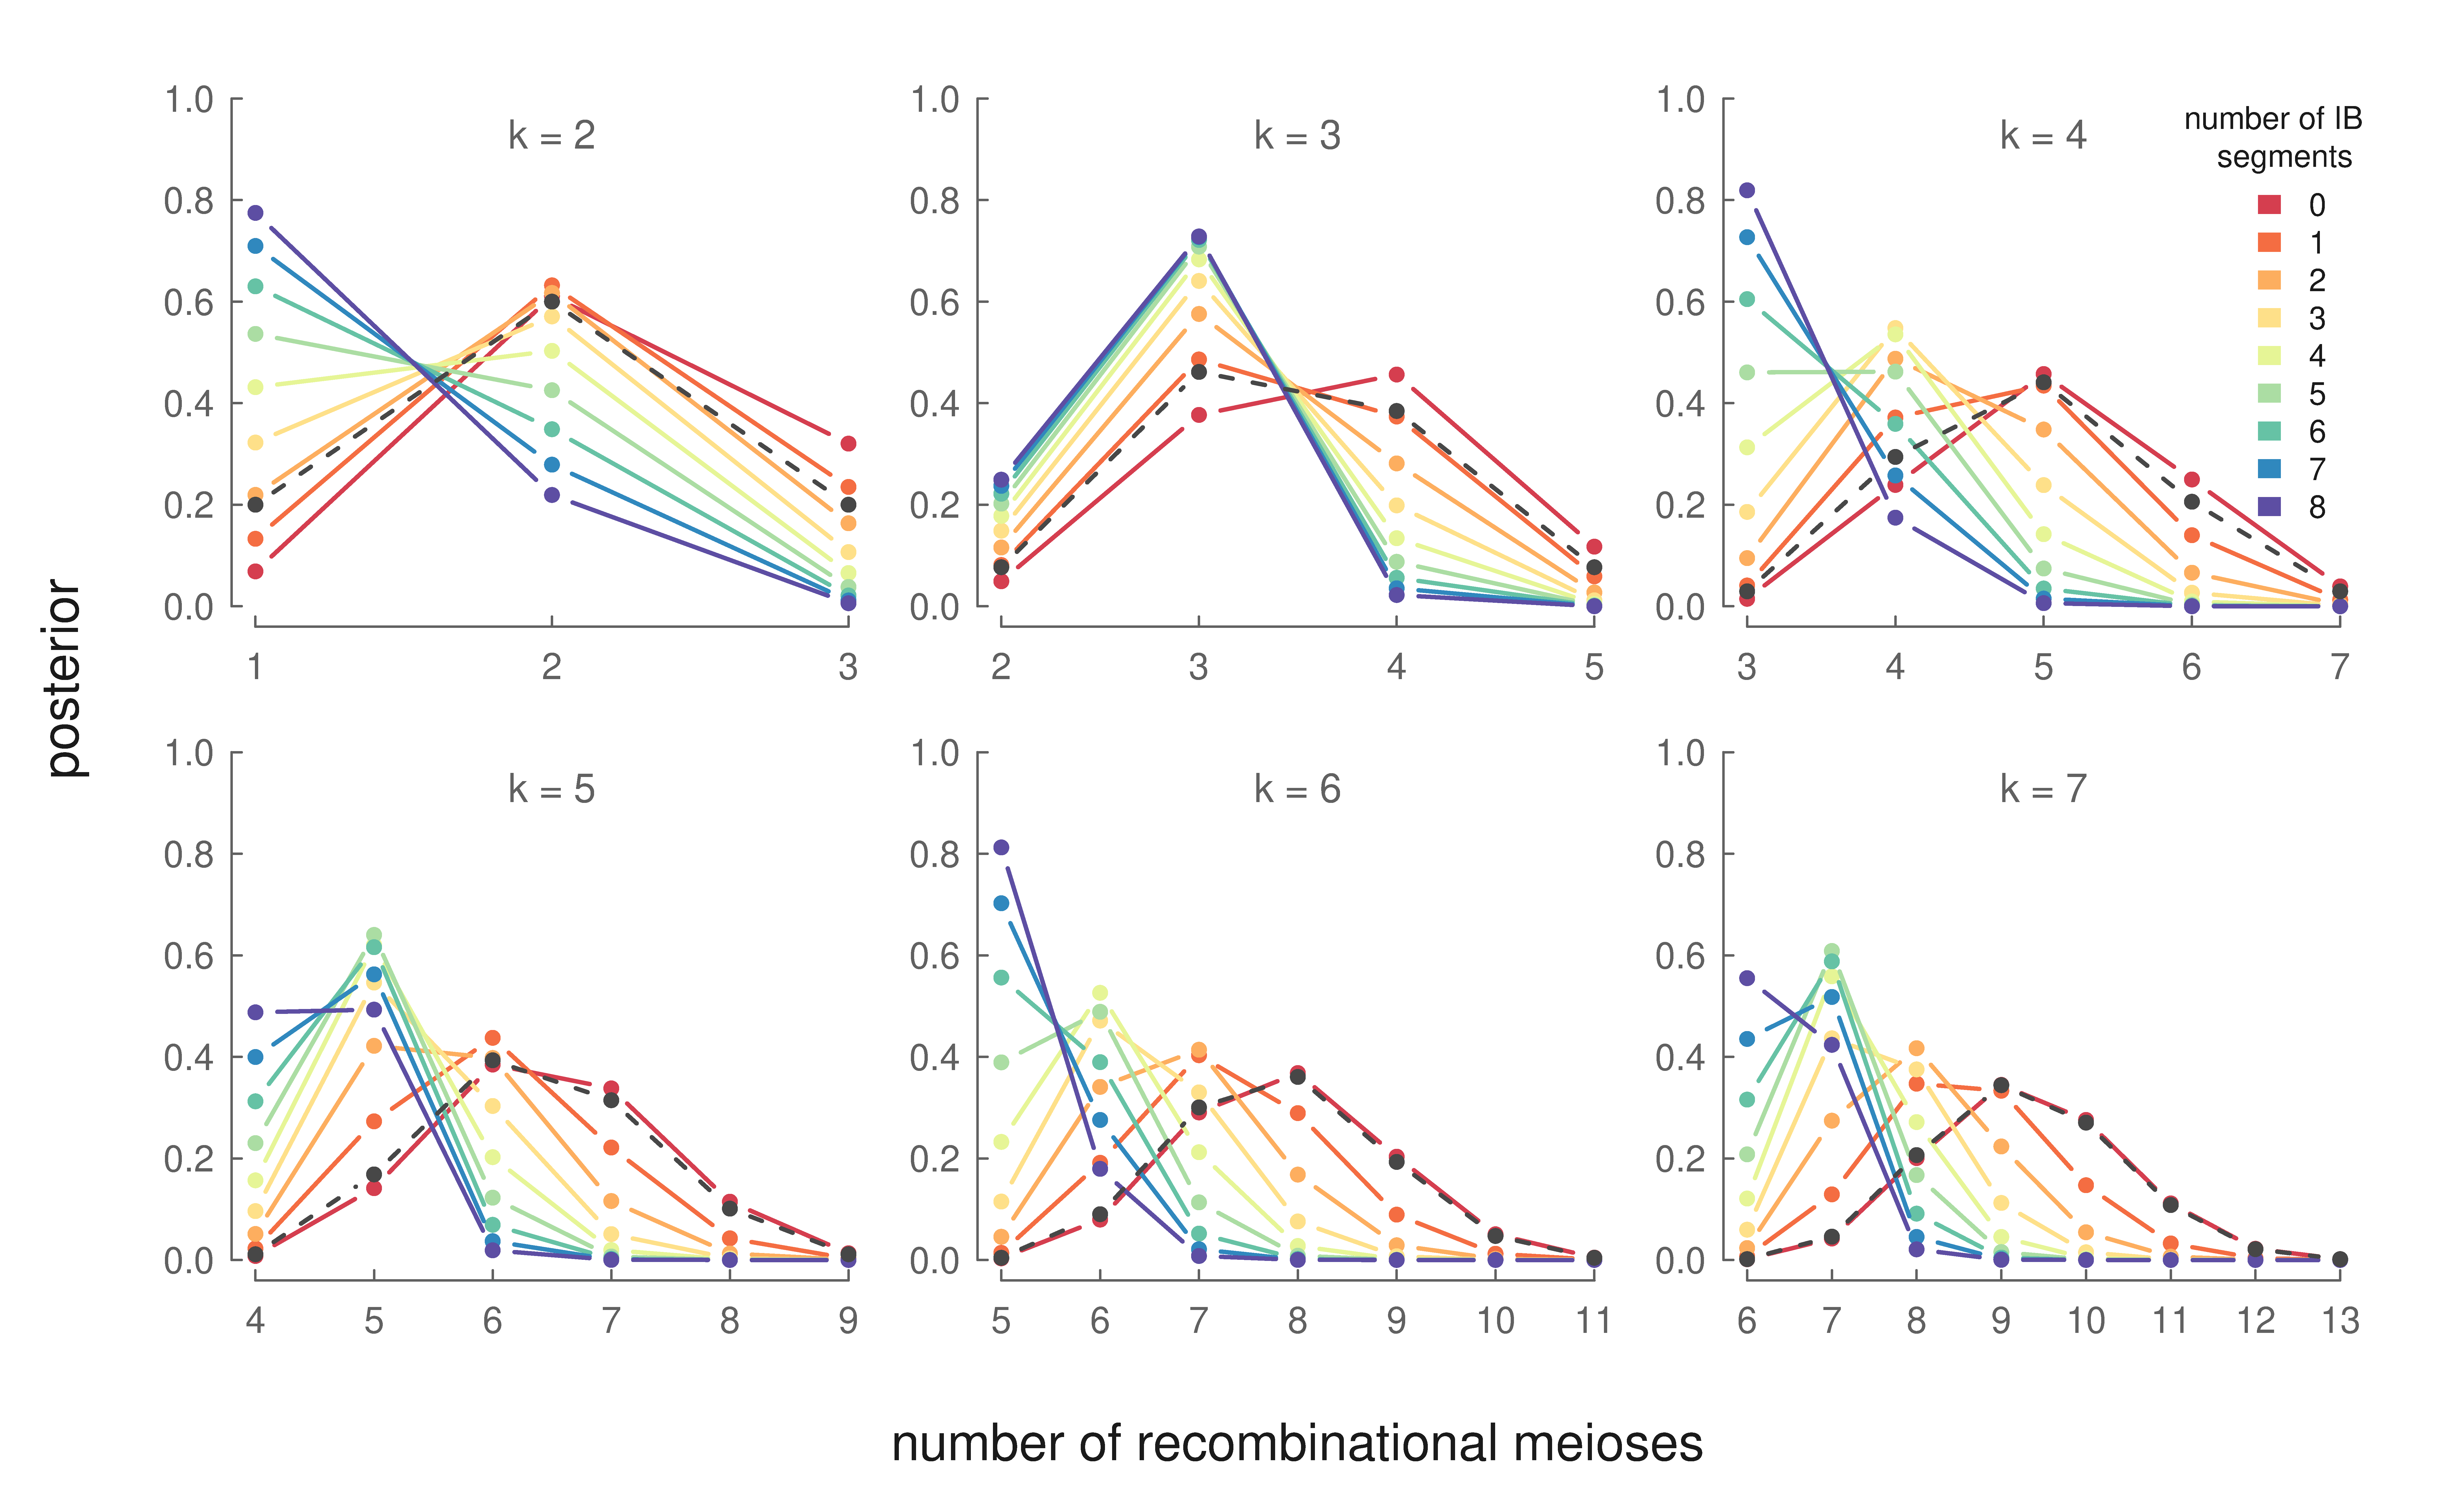
\includegraphics[width=\linewidth]{figures/chapter_1/rm-posterior}

  \caption[Posterior probability distribution of recombinational meioses given
  number of shared X IBD segmnets observed]{Posterior probability distribution
    $P(R = r | N = n, k)$ for different generations (each panel), and the
    observed number of IBD segments (each colored line). The prior distribution
  of recombinational meioses given $k$ is indicated by a black dashed line.}

  \label{fig:inference}

\end{figure*}

In Figure \ref{fig:inference}, we show the posterior distributions over the
number of recombinational meioses, given an observed number of IBD segments
between two females known to be X half-cousins. Again, these posterior
distributions condition on knowing how many generations have occurred since the
shared ancestor, $k$.  With an increasing number of generations to the shared
ancestor, fewer segments survive to be IBD between the present-day cousins.
Consequently, observing IBD segments increases the likelihood of fewer females
(and thus fewer recombinational meioses) between the cousins. For example, for
$k=6$, observing (the admittedly unlikely) six or more IBD segments leads to a
posterior mode over the fewest possible number of females in the genealogical
chain ($\lfloor (2k-1)/2 \rfloor = 5$; Figure \ref{fig:inference}).  Similarly,
observing between three and five segments places the posterior mode over six
females in the genealogical chain. For $k>4$, seeing zero segments provides
little information over the prior about the relationship between the cousins,
as sharing zero segments is the norm. In each case, a posterior distribution
over the number of females in a genealogical chain can greatly reduce the
number of likely genealogical configurations. For example, observing $n=3$
shared X segments between half-cousins $k=4$ generations back first restricts
their shared ancestor to be one of the $34$ possible shared X ancestors (out of
the total $128$ possible shared ancestors). Furthermore, these three shared X
segments combined with our posterior distribution over recombinational meioses,
leads to a \emph{maximum a posteriori} estimate of $\hat{R} = 4$ females along
the genealogical chain connecting the half-cousins. Only 10 genealogical chains
connecting these cousins contain four females, thus the likely relationship of
these cousins is considerably narrowed from the original 128 possible
relationships. Therefore, sharing genetic segments on the X can provide
considerable information about genealogical relationships.

\section{Discussion}

Detecting and inferring the nature of recent ancestry is important to a range
of applications and the nature of such relationships are often of inherent
interest. As the sample sizes of population genomic data sets increase, so will
the probability of sampling individuals that share recent ancestry. In
particular, the very large data sets being developed in human genetics will
necessitate taking a genealogical view of recent relatedness.  Our methods
extend existing methods for the autosomes by accounting for the special
inheritance pattern of the X. Specifically, recent ancestry on the X differs
from the autosomes since males only inherit an X from their mothers, and
fathers pass an unrecombined (ignoring the PAR) X to their daughters.
Consequently, the number of recombinational meioses, which determine the length
and number of IBD segments, varies across the X genealogy. Since in most cases
the number of females between two individuals in a genealogical chain is often
unknown, we derive a distribution for recombinational meioses (equation
\eqref{eq:recomb-pmf}).

We also derive distributions for the length and number of IBD X segments by
marginalizing over the unknown number of recombinational meioses that can occur
between two individuals connected through a genealogical chain. In both cases,
we condition on knowing $k$ (the generations back to a shared ancestor) which
can be inferred from the autosomes \parencite{huff2011maximum}. Our models for IBD
segment number and length use a Poisson-Binomial approximation to the
recombination process, which match simulation results closely.

The genomic information about the genealogical relationship between pairs of
individuals is inherently limited (due to the small number of segments shared
and the stochasticity of the process); thus making full use of all shared
segments on all chromosomes will be key to better inference. Our results here
not only allow X IBD segments to be used to model recent ancestry, but in fact
provide qualitatively different informative about genealogical ancestry than
autosomal data alone. This additional information occurs through two avenues.
First, sharing IBD segments on the X immediately reduces the potential
genealogical ancestors two individuals share, since one's X ancestors are only
a fraction of their possible genealogical ancestors (i.e.
$\mathcal{F}_{k+2}/2^{k}$ in the case of a present-day female). Second, the
varying number of females in an X genealogy across lineages combined with the
fact that recombinational meioses only occur in females to some extent leave a
lineage-specific signature of ancestry.

Unfortunately, the X chromosome is short, such that the chance of any signal of
recent ancestry on the X decays rather quickly. However, growing sample sizes
will increase both the detection of the pairwise relatedness and cases of
relatedness between multiple individuals. In these large data sets, overlapping
pairwise relationships (e.g. a present-day individual that shares X segments
with two distinct other individuals) could be quite informative about the
particular ancestors that individuals share. 

Our results should also be of use in understanding patterns of admixture on the
X chromosome. In particular our results about the posterior information from
the number and length of X segments shared with a genealogical ancestor can
help us understand what can be learned from the presence (or absence) of
segments of particular ancestry on the X chromosome. For example, if you
observed long segments of a particular ancestry on your X chromosome our
results could be used to aid the identification of which parts of your family
tree this ancestry has been inherited from. These genetic genealogical
inferences can provide informative details in genealogy reconstruction where
historical genealogical information is missing or uncertain. While this
information for an individual decays somewhat quickly after a small number of
generations, models of X chromosome segment ancestry will be useful at a
population-level for understanding sex-biased admixture
\parencite{bryc2010genome,Goldberg:2015ja,Shringarpure039347}.

\newpage
%\appendix

\section{Convergence of the Thinned Poisson Process to Poisson-Binomial Model}
\label{ap:pois-thin}

We compared the Poisson thinning approximation and the Poisson-Binomial models.
One can show using the law of total expectation that the Poisson-Binomial and
Poisson model have the same expected value:

\begin{align*}
  \E[N] &= \sum_{b=0}^\infty \E[N | B = b]P(B = b) \nonumber\\
  \E[N] &= \frac{1}{2^d} \left( \sum_{b=0}^\infty b \text{Pois}(B = b) + c \sum_{b=0}^\infty \text{Pois}(B = b) \right)  \nonumber\\
  \E[N] &= \frac{1}{2^d} (\nu d + c) 
\end{align*}
%
This is the same expected value as the thinned Poisson process with rate $(\nu
d + c)/2^d$. However, the Poisson thinning and Poisson-Binomial models differ
in their variance. Using Eve's law, we can show the Poisson-Binomial model has
variance
%
\begin{align*}
  \V[N] &= \E_B[\V[N | B]] + \V_B[\E[N|B]]  \nonumber\\
  \V[N] &= \frac{dv + 1}{2^d} - \frac{1}{2^{2d}}
\end{align*}
%
This differs from the thinned Poisson process variance by the term
$\nicefrac{1}{2^{2d}}$, which grows smaller with increasing $d$. Finally, we
numerically show these two distributions (here, we label the two distributions
for $k$ generations $\mu_k(x)$ and $\nu_k(x)$, where $x$ is the number of
segments) converge quickly in total variational distance ($d_{TV}(\mu_k, \nu_k) =
\nicefrac{1}{2}\sum_{n = 0}^\infty | \mu_k(n) - \nu_k(n) |$) as $k$ increases,
in Figure \ref{fig:total-var-dist}.

\begin{figure}[!ht]
  \centering
  
\includegraphics[width=\linewidth]{figures/chapter_1/total-var-dist}

  \caption[Total variation distance between Poisson thinning approximation and
  the Poisson-Binomial model]{The total variation distance between the Poisson
  thinning and the Poisson-Binomial model for IBD segment number for X segments
(yellow) and the autosomal segments (blue).}

\label{fig:total-var-dist}
\end{figure}

\section{Additional Autosomal Segment Distributions}
\label{ap:auto-cousin}
\subsection{The distribution of IBD segments between cousins}

Similar to the distribution of autosomal segments between a present-day
individual and an ancestor (Section \ref{sec:auto-dist-ibd-seg}), we can derive
the distribution for the number of IBD segments shared between two half-cousins
with an ancestor in the $k^\text{th}$ generation. Two half-cousins are
separated by $2k$ meioses, thus the distribution for number of segments is:

\begin{equation}
  \label{eq:auto-seg-cousins}
  P(N=n \;|\; k, \nu, c) = \text{Pois}\left(N = n \;|\; \lambda=(c + 2 k \nu)/2^{2 k - 1} \right)
\end{equation}
%
Since either of the shared ancestor's haplotypes can be shared IBD between the
two cousins, the Poisson process rate is doubled. Full-cousins can share segments
via either of their two shared ancestors, leading the distribution to be:

\begin{equation*}
  P(N=n \;|\; k, \nu, c) = \text{Pois}\left(N = n \;|\; \lambda=(c + 2 k \nu)/2^{2 k - 2} \right)
\end{equation*}


\subsection{The distribution of autosome segment lengths}

In addition to the number of IBD segments, the length of segments is also
informative about ancestry \parencite[e.g.][]{palamara2012length}. As we model
crossing over as a Poisson process, a one Morgan region will experience on
average $d$ recombination events over $d$ meioses. Therefore, the probability
density of segment lengths shared IBD between two individuals $d$ meioses apart
is exponential with rate $d$:

\begin{equation}
  \label{eq:auto-seg-lens}
  p(U=u | d) = d e^{-du}
\end{equation}

Equations \eqref{eq:auto-seg-lens} and \eqref{eq:auto-seg-cousins} specify a
model of the number and lengths of segments shared between various degree
relatives. Various authors have used these types of results to derive
likelihood-based models for classifying the genealogical relationship between
pairs of individuals using autosome IBD data
\parencite{huff2011maximum,Henn:2012ij,Durand010512}. 

\section{Generating Function for Recombinational Meioses}
\label{ap:generating-function}

We also develop a generating function $g(x, k)$ that encodes the number of
recombinational meioses in the $k^{\text{th}}$ generation as the coefficient
for the term $x^k$. This generating function can also be used in approximations
and finding moments of the distribution $p_k(r)$.

An expansion of the generating function below encodes the number of lineages
with $r$ females in a genealogical chain $k$ generations long ($n_{k,r}$) as
the coefficient of the term $x^{k}$

\begin{align*}
  g(x, k) = \frac{1}{2^{k+1}\sqrt{x} \sqrt{x+4}} &\left[ x 
    \left(\left(R^+\right)^k - \left(R^-\right)^k\right)  \right. \nonumber\\
    &+ \sqrt{x} \sqrt{x+4}
    \left(\left(R^-\right)^k + \left(R^+\right)^k\right)  \nonumber\\
    &+ \left. -2 \left(R^-\right)^k+2 \left(R^+\right)^k\right]
\end{align*}

\text{where}

\begin{align*}
    R^- &= x-\sqrt{x} \sqrt{x+4}\\
    R^+ &= x+\sqrt{x} \sqrt{x+4}
\end{align*}

\begin{proof}

 We begin by stating some recurrences that occur from the inheritance pattern of
 X ancestry:

\begin{subequations}
  \label{eq:gen-recur}
  \begin{align}
    n_{k,r} &= m_{k,r} + f_{k,r} \label{eq:recur-01}\\
    m_{k,r} &= f_{k-1,r} \label{eq:recur-02}\\
    f_{k,r} &= f_{k-1, r-1} + m_{k-1,r-1} \label{eq:recur-03}\\
  \end{align}
\end{subequations}

Starting from equation \eqref{eq:recur-01}:

\begin{align*} 
   n_{k,r} &= m_{k,r} + f_{k,r} \\
   n_{k,r} &= f_{k-1,r} + f_{k,r} \\
   n_{k,r} &= f_{k-1,r} + f_{k-1, r-1} + m_{k-1,r-1} \\
   n_{k,r} &= f_{k-1,r} + n_{k-1, r-1} \\
   n_{k,r} &= f_{k-2, r-1} + m_{k-2,r-1} + n_{k-1, r-1} \\
\end{align*}

%% TODO
finally, substituting equation \eqref{eq:recur-01} again gives us the desired
recurrence relation for $n_{k,r}$:

\begin{equation} 
   \label{eq:genrecur}
   n_{k,r} = n_{k-2, r-1} + n_{k-1, r-1}
\end{equation}

We can now use generating functions \parencite{wilf2013generatingfunctionology} to
tackle this recurrence. Define:

\begin{equation*}
  A_k(x) = \sum_{r \ge 0} n_{k,r} x^r
\end{equation*}

then, multiply both sides of \eqref{eq:genrecur} by $x^r$ and sum over $r$. On
the right hand side:

\begin{align*}
  &= \sum_{r \ge 0} n_{k-2, r-1} x^r + \sum_{r \ge 0} n_{k-1, r-1} x^r
\end{align*}

 Note that $n_{k,r} = 0$ if $r < 0$. Multiplying and dividing the second term by
 $x$ yields:

 \begin{align*}
   x(n_{k-1, 0} x + n_{k-1, 1} x^2 + n_{k-1, 2} x^3 + \ldots)/x = x A_{k-1}(x) 
 \end{align*}

 An identical derivation works for the first term. We find:

 \begin{equation*} \label{eq:rec-gen}
   A_k(x) = xA_{k-1}(x) + xA_{k-2}(x)
 \end{equation*}

This generating function is in the form of another recurrence. We can solve
this recurrence (i.e. with Mathematica) with the initial conditions below
(which can be derived from \eqref{eq:recur-01} and its initial conditions)
%
\begin{enumerate}
  \item $ A_0(x) = 1 $
  \item $ A_1(x) = 1 + x $
\end{enumerate}
%
to find a solution with these initial conditions, giving us our desired
generating function $g(x,k)$.

\end{proof}

We can see that our generating function works via an expansion and verify
the coefficients match known numbers of recombinational meioses for some $k$.
For example, let's expand $g(x, k)$ at $k=5$:

\begin{equation*}
  x^2 + 6x^3 + 5x^4 + x^5
\end{equation*}
%
which matches the $n_{k,r}$ values found via computational calculation.

\section{Half-Cousins IBD Length Distribution Simulation Results}

Figure \ref{fig:half-cousin-x-length} show the concordance between our cousin
IBD segment length analytic distributions and the binned average (1.98cM bin
intervals) of 5,000 simulations.

\begin{figure*}[!ht]
  \centering
  
\includegraphics[width=\textwidth]{figures/chapter_1/x-halfcousins-blocklens}

  \caption[The analytic distributions of X IBD segment length between two
  present-day female half-cousins with a shared ancestor]{The analytic
    distributions of IBD segment length (blue lines) between two-present-day
    female half-cousins with a shared ancestor in the $k^\text{th}$ generation
  (each panel), and the binned average 5,000 simulations (gray points).}

\label{fig:half-cousin-x-length}

\end{figure*}

\section{An Approximation of X Pedigree Collapse}
\label{ap:ped-collapse}

Since our models of recent X ancestry omit the possibility of pedigree
collapse, it is worthwhile to see when this assumption breaks down. To see how
pedigree collapse becomes an increasing problem further generations back, we
look at the probability that all of a single individual's $\mathcal{F}_{k+2}$ X
ancestors, when sampled from a population of $N$ individuals with replacement,
are distinct. We treat generations as discrete and non-overlapping, and look at
the probability that all $\mathcal{F}_{k+2}$ are distinct individuals as a
function of how many generations we go back. This problem is similar to the
celebrated birthday problem, but with two rooms of participants: one room of
females and another of males. Assuming random mating, each generation, one's X
ancestors must be randomly selected with replacement from a population of $N$
individuals. For all ancestors to be distinct, all $\mathcal{F}_{k}$ male
ancestors selected from a pool of $N/2$ and $\mathcal{F}_{k+1}$ female
ancestors selected from a pool of $N/2$ must be unique:

\begin{align*}
  P(\text{X ancestors all distinct}) &= P(\text{male X ancestors unique})   \nonumber\\
  & \;\; \times P(\text{female X ancestors unique}) \nonumber\\
                                     &= \prod_{i=1}^{\mathcal{F}_{k}} \left(1-\frac{2i}{N}\right)\prod_{j=1}^{\mathcal{F}_{k+1}} \left(1-\frac{2j}{N}\right)
\end{align*}

This probability as a function of $k$ is plotted in Figure
\ref{fig:ped-collapse}. For X ancestors, the probability that at least two
individuals are non-distinct only becomes a significant problem after around 12
generations. Note that this is a very conservative account of how pedigree
collapse could affect our calculations; even if two ancestors were to be
non-distinct, this is unlikely to affect our calculations greatly. For pedigree
collapse to affect our IBD segment models, an individual has to both be a
genealogical ancestor \emph{and} a genetic ancestor of the present-day
individual; pedigree collapse has no genetic affect if non-distinct individuals
are not genetic ancestors.

\begin{figure}[!ht]
  \centering
  
\includegraphics[width=\linewidth]{figures/chapter_1/ped-collapse}
  \caption[The probability of distinct genealogical and X ancestors]{The probability that all genealogical and X ancestors are distinct in a population of $N=100,000$.}
  \label{fig:ped-collapse}
\end{figure}

For other pedigree collapse related quantities (e.g., what's the average number
of distinct ancestors $k$ generations back), see
\textcite{wachter2013statistical} approximations which use Feller's
(\citeyear{feller1950introduction}) occupancy models.


%\addbibresource{temporal-covariance.bib}

\chapter{The Linked Selection Signature of Rapid Adaptation in Temporal Genomic Data}
\counterwithin{figure}{chapter}

Adaptation can occur over remarkably short ecological timescales, with
dramatic changes in phenotype occurring over just a few generations in natural
populations. This rapid pace of adaptive change has been known to be mirrored
at the genetic level since the early work of \textcite{Fisher1947-tf}  testing
whether the rapid decline in a coloration polymorphism was consistent with
natural selection or genetic drift. Since then, researchers have continued to
use temporal data to detect selection on polymorphisms over short timescales in
natural populations
\parencite{Kettlewell1958-or,Kettlewell1961-ok,Fisher1947-tf,Dobzhansky1943-lh,Dobzhansky1971-vf,Mueller1985-eo},
as well as quantify the rate of genetic drift
\parencite{Nei1981-oy,Pollak1983-xh,Mueller1985-eg,Waples1989-sj,Wang2003-ev,Prout1954-yy,Wallace1956-jb}.
However, this line of work in sexual populations has been partially eclipsed by
a vast body of work examining large-scale population-genetic and -genomic data
sets from a single contemporary timepoint. More recently, studies have applied
similar temporal approaches to whole-genome data to discover selected loci in
contemporaneous natural populations
\parencite{Bergland2014-ij,Rajpurohit2018-od}, evolve and re-sequence studies
\parencite{Burke2010-tz,Johansson2010-ya,Teotonio2009-sa,Turner2011-sx,Turner2012-bm,Franssen2017-lx,Orozco-terWengel2012-fu,Barghi2019-qy},
and ancient DNA \parencite{Mathieson2015-uw,Fu2016-ek}. Furthermore,
  numerous methods have been developed to estimate effective population size
\parencite{Pollak1983-xh,Waples1989-sj,Nei1981-oy} and detect selected loci
\parencite{Feder2014-lc,Mathieson2013-we,Terhorst2015-rg,Malaspinas2012-aw}
from time-series data.

Overall, these approaches have identified compelling examples where selection has driven
extreme allele frequency change at particular loci that is inconsistent with
drift alone.  However, most adaptation on ecological timescales likely involves
selection on phenotypes with polygenic architecture and abundant standing
variation \parencite{Endler1986-wd,Hendry1999-zu,Kinnison2001-vb,Kopp2009-pj}.
We know from theory that adaptation on such traits can result from very subtle
allele frequency changes across the many loci that underlie the trait
\parencite{Bulmer1980-zo}, at least for the short-term evolutionary response
\parencite{Jain2017-mw,Jain2015-xy,Thornton2018-eo,Chevin2008-lt,Hermisson2005-hs,Hollinger2019-mn}.
These changes may be individually indistinguishable from genetic drift in
temporal data. This poses a challenge for population genetic approaches to
quantify selection: rapid phenotypic adaptations occurring on ecological
timescales may leave a signal on genome-wide patterns of diversity that is
undetectable by methods focused on individual loci.

Here, we explore an alternative: rather than aiming to find selected loci, we
can use temporal data to quantify the genome-wide effects of linked selection
during polygenic adaptation. Linked selection introduces a new source of
stochasticity into evolution, as a neutral allele's frequency change depends on
the fitness of the set of random genetic backgrounds it finds itself on
\parencite{Gillespie2000-mh}. The impact linked selection has on neutral loci
is mediated by associations (linkage disequilibria, or LD) with selected loci
and hence their recombination environment; neutral loci tightly linked to
selected sites experience greater average reductions in diversity than more
loosely coupled sites. Studies using a single timepoint have long exploited
this idea, with some of the first evidence of pervasive natural selection being
the correlation between diversity and recombination in \emph{Drosophila}
\parencite{Aguade1989-jx,Begun1992-ey}. Various forms of linked selection give
rise to such patterns with much attention focusing on the hitchhiking (positive
selection; \cite{Maynard_Smith1974-lc}), or background selection models
(negative, or purifying selection; \cite{Charlesworth1993-gb,Hudson1995-xc}).
Recent genomic studies have modeled patterns of genome-wide diversity
considering substitutions, functional constraint, and recombination
environments to estimate parameters of hitchhiking and background selection
models, and have begun to differentiate between these models
\parencite{McVicker2009-ax,Hernandez2011-gs,Elyashiv2016-vt}.  Across-taxa
comparisons have shown that signals of linked selection are present in many
sexual organisms, and that in some species a proportion of the stochastic
change in allele frequencies is due to the randomness of linked selection
instead of genetic drift
\parencite{Cutter2013-ba,Corbett-Detig2015-gt,Coop2016-gx}. Likewise, in
asexual and facultatively sexual organisms both theory and empirical work show
that linked selection and interference are a primary determinant of the levels
of genetic diversity
\parencite{Neher2011-fy,Neher2013-dz,Good2017-om,Good2014-yz}.

In this paper, we extend this well-established approach of quantifying
genome-wide selection through its indirect impact on linked neutral sites to
temporal genomic data. We show that during rapid polygenic selection, linked
selection leaves a signal in temporal genomic data that can readily be
differentiated from neutral processes. Specifically, selected alleles perturb
the allele frequency trajectories of neighboring neutral loci, increasing the
variance of neutral allele frequency change and creating covariance between the
neutral allele frequency changes across generations.  Earlier work has modeled
this effect on neutral alleles as a long-term reduction in the effective
population size
\parencite{Robertson1961-ho,Santiago1995-hx,Santiago1998-bs,Wray1990-zf,J_A_Woolliams_N_R_Wray_R_Thompson2008-qo},
but the increasing availability of genome-wide frequency data across multiple
timepoints allows us to directly quantify the extent of linked selection over
short ecological timescales (tens of generations). We develop theory for the
variances and covariances of neutral allele frequency change under selection,
and show that analogous to diversity in a single timepoint study, their
magnitude depends on the local fitness variation, recombination, and linkage
disequilibria. Furthermore, we show that our theory can (1) directly
partition the variation in genome-wide frequency change into the components
caused by drift and selection, (2) estimate the additive genetic
variance for fitness and how it changes over time, and (3) detect patterns of
fluctuating selection from temporal data. Overall, we believe our approach to
modeling temporal genomic data will provide a more complete picture of how
selection shapes allele frequency changes over ecological timescales in natural
populations, potentially allowing us to understand short-term effects of linked
selection that would otherwise not be perceptible from studies using a single
timepoint. 

\section{Outline of Temporal Autocovariance Theory}
\label{sec:outline-temp}

Our goal is to understand how linked selection affects the frequency
trajectories of neutral sites by modeling the variances and covariances of
neutral allele frequency changes ($\Delta p_t = p_{t+1} - p_t$, where $p_t$ is
the population frequency at time $t$). We assume a closed population with
discrete, non-overlapping generations. When there are no heritable fitness
differences between individuals, genetic drift is the only source of
stochasticity of allele frequency change due to two sources of variation:
random non-heritable, or environmental differences in offspring number, and
Mendelian segregation of heterozygotes. Both are directionless such that when
averaged over evolutionary replicates, the expected change in allele frequency
due to drift alone is $\E(\Delta p_t) = 0$ and quantified by the variance in
allele frequency change $\var(\Delta p_t)$ \parencite[as quantified by the
variance effective population
size;][]{Wright1938-tv,Crow1970-wm,Charlesworth2009-sg}.

% We first give an outline of how selection affects linked neutral sites through
% time. We summarize a neutral allele's frequency trajectory as the differences
% in adjacent timepoints, $\Delta p_t = p_{t+1} - p_t$, where $p_t$ is the
% population frequency at time $t$, and we assume a closed population with
% discrete, non-overlapping generations. While throughout the paper we assume
% that allele frequencies can be measured every generation, the same approach can
% be extended to situations where the study system cannot be observed every
% generation. Our goal is to understand how linked selection affects the
% frequency trajectories of neutral sites by modeling the variances and
% covariances of neutral allele frequency changes. Before considering the impact
% of linked selection, we first consider a population that lacks heritable
% fitness differences between individuals. In this case, the stochasticity of
% allele frequency change is determined entirely by two components: random
% non-heritable, or environmental differences in offspring number, and Mendelian
% segregation of heterozygotes. These two sources of stochasticity are
% collectively known as drift, and both are directionless such that when averaged
% over evolutionary replicates, the expected change in allele frequency due to
% drift alone is $\E(\Delta p_t) = 0$. The magnitude of drift's stochastic
% effects are quantified by the variance in allele frequency change $\var(\Delta
% p_t)$, which in a Wright--Fisher model of reproduction where offspring number
% has a multinomial distribution, is $\var(\Delta p_t) =
% \nicefrac{p_t(1-p_t)}{(2N)}$. Different mating systems and higher non-heritable
% variance in offspring number can be accommodated under the Wright--Fisher model
% by replacing $N$ with $N_e$, the variance effective population size
% \parencite{Wright1938-tv,Crow1970-wm,Charlesworth2009-sg}.

When there are heritable fitness differences between individuals in the
population, a third source of stochasticity affects a neutral allele's
frequency change: neutral alleles can become randomly associated with the
genetic backgrounds that determine the fitness differences between individuals
\parencite{Robertson1961-ho,Santiago1995-hx,Santiago1998-bs}. Even though the
neutral alleles do not impact fitness, their frequency trajectories are
perturbed by their fitness background, as those on advantage backgrounds leave
more descendants, while those on disadvantageous backgrounds leave fewer. We
can partition a neutral allele frequency's change into these three uncorrelated
stochastic components (following \citeauthor{Santiago1995-hx},
\citeyear{Santiago1995-hx}, see our Appendix Section \ref{ap:decomp} for
proof),

\begin{align}
  \Delta p_t %&= p_{t} - p_{t-1}  \\
  &= \underbrace{\Delta_{_N} p_t + \Delta_{_M} p_t}_\text{drift} + \underbrace{\Delta_{_H} p_t}_\text{selection}
  \label{eq:delp-decomp}
\end{align}
%
where, $\Delta_{_N} p_t$, $\Delta_{_M} p_t$, and $\Delta_{_H} p_t$ are the
neutral allele's frequency changes due to non-heritable variation in fitness
between diploid individuals, Mendelian segregation of heterozygotes into
offspring, and heritable variation in fitness (we refer to this as the
\emph{heritable change} in neutral allele frequency), respectively. Note that 
  while throughout the paper we consider the allele frequency change between
  adjacent generations, the same approach can be extended to situations where
the study system cannot be observed every generation. Like the stochastic
components of drift, the allele frequency change due to heritable fitness
differences is directionless ($\E(\Delta_{_H} p_t) = 0$).
Additionally, since each component is uncorrelated with the others, the
variance in allele frequency change is

\begin{align}
  \var(\Delta p_t) &= \var(\Delta_{_N} p_t)  + \var(\Delta_{_M} p_t) + \var(\Delta_{_H} p_t).
  \label{eq:var-decomp-1}
\end{align}
%
The terms $\var(\Delta_{_N} p_t)$ and $\var(\Delta_{_M} p_t)$ capture the
variance due to the random reproduction process, and the former can accommodate
extra non-heritable variance in offspring number (as long as individuals are
exchangeable with respect to their genotype; \cite{Cannings1974-ps}), while the
term $\var(\Delta_{_H} p_t)$ captures heritable fitness variation due to
systematic differences in the fitness of individuals caused by their genotypes.

In addition to inflating the within-generation variance in allele frequency
change, heritable fitness variation has another profound affect on neutral
alleles: while the stochastic components of drift have independent effects on
frequency change each generation, heritable variation in fitness creates
\emph{temporal autocovariance} in neutral allele frequency changes across
generations. The contribution of temporal autocovariance is evident by writing
the total cumulative allele frequency change as the sum of allele frequency
changes each generation,

\begin{align}
  \label{eq:var-decomp}
  \var(p_t - p_0) &= \var(\Delta p_{t-1} + \Delta p_{t-2} + \ldots + \Delta p_0) \nnn \\
                  &= \sum_{i=0}^{t-1} \var(\Delta p_i) + \sum_{i \ne j} \cov(\Delta p_{i}, \Delta p_{j}) \nnn \\
  \var(p_t - p_0) &= \underbrace{\sum_{i=0}^{t-1} \left(\var(\Delta_{_N} p_i) +  \var(\Delta_{_M} p_i) \right)}_\text{drift} +  \nonumber\\ 
                  &\underbrace{\sum_{i=0}^{t-1} \var(\Delta_{_H} p_i)}_\text{genetic variance in offspring number} + \underbrace{\sum_{i \ne j} \cov(\Delta_{_H} p_i, \Delta_{_H} p_j)}_\text{temporal autocovariance}.
\end{align}
%
These covariance terms are expected to be non-zero only when there is heritable
variation in fitness (assuming there is neither non-Mendelian segregation nor
covariance between parental and offspring environment, e.g. as in
\cite{Heyer2005-cl}).

\begin{figure}[!ht]
  \centering
  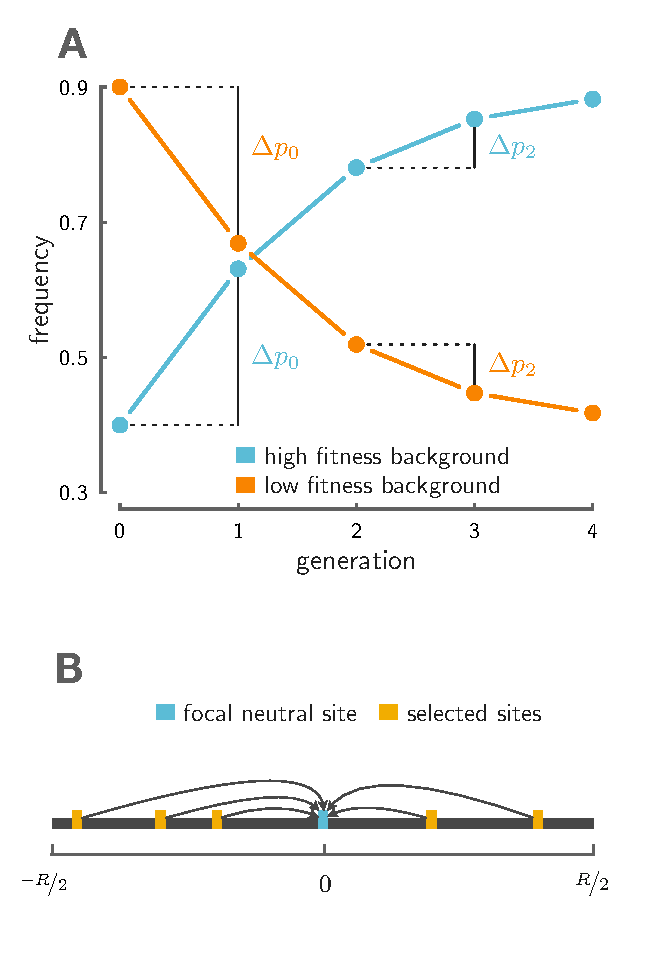
\includegraphics[width=0.5\textwidth]{./figures/keynote-cartoons-figure-1.pdf}

  \caption[Cartoon of the trajectories of neutral alleles with temporal
  autocovariance, and schemetic of our multilocus setup]{A: On an advantageous
    background (light blue), a neutral allele increases in frequency leading to
    a positive change in allele frequency early on, $\Delta p_0 = p_1 - p_0$.
    As long as some fraction of neutral alleles remain associated with this
    advantageous background, the neutral allele is expected to increase in
    frequency in later generations, here, $\Delta p_2 = p_3 - p_2$. This
    creates temporal autocovariance, $\cov(\Delta p_2, \Delta p_0) > 0$.
    Similarly, had the neutral allele found itself on a low-fitness background
    (orange), this would also create temporal autocovariance.  B: This depicts
    the setup for our multilocus model.  Multiple alleles (yellow) determine
    the fitness in a region $R$ Morgans in length, and these perturb the allele
    frequency trajectory of a focal neutral site (light blue).  }
  \label{fig:cartoon} \end{figure}

Temporal autocovariance is caused by the persistence over generations of the
statistical associations (linkage disequilibria) between a neutral allele and
the fitnesses of the random genetic backgrounds it finds itself on; as long as
some fraction of associations persist, the heritable variation for fitness in
one generation predicts the change in later generations, as illustrated by the
fact that $\cov(\Delta p_2, \Delta p_0) > 0$ (see Figure \ref{fig:cartoon}A).
Ultimately segregation and recombination break down haplotypes and shuffle
alleles among chromosomes, leading to the decay of autocovariance with time. 

The effect heritable variation has on neutral alleles has traditionally been
modeled in a quantitative genetics framework where a large number of loosely
linked polymorphisms contribute to heritable fitness differences between
individuals, and the impact of heritable fitness variation on a neutral allele
is quantified as a reduction in its long-run effective population size
\parencite{Robertson1961-ho,Santiago1995-hx,Santiago1998-bs}.  This form of
linked selection can be contrasted with classic population genetic hitchhiking
theory (\cite{Maynard_Smith1974-lc}), which considers how neutral alleles
closely linked to a new beneficial mutation are affected as it sweeps to
fixation. While classic population genetic linked selection models consider how
neutral variation is affected by strong associations caused by tight linkage to
an advantageous site, quantitative genetic models of linked selection
considered the weakest forms of associations: those between unlinked loci
within an individual (\cite{Morley1954-yp, Robertson1961-ho, Santiago1995-hx};
see \cite{Barton2000-zg} for more on the two models of linked selection). These
distant associations are quickly established but are rapidly broken down by
segregation and independent assortment, yet still can have a marked effect on
diversity \parencite{Robertson1961-ho,Santiago1995-hx}. However, since the
impact of heritable fitness variation has traditionally been modeled as causing
a reduction in the effective population size, there has been no direct way to
separately estimate its effects from those of drift. We show that with temporal
genomic data, one can directly measure the levels of temporal variances and
autocovariances of allele frequency change in the population. Additionally, we
that show temporal autocovariance is created under both tight and loosely
linked selection, and below, develop expressions for its magnitude that are
applicable to both, bridging the two regimes of linked selection.

\section{A model for multilocus temporal autocovariance}

Here, we develop theory for the temporal autocovariance in a neutral allele's
frequency changes through time, generated by the presence of heritable fitness
in the population. We measure the temporal autocovariance $\cov(\Delta p_t,
\Delta p_s)$ at a single diallelic neutral locus. Since only allele frequency
changes due to heritable variation in \emph{fitness} contribute to temporal
autocovariance, we can focus exclusively on the behavior of $\Delta_{_H} p_t$
in deriving our expressions for the autocovariance across timepoints. We
imagine that an individual $i$ has fitness $f_i$, i.e. that their expected
number of children is $f_i$. We assume a constant population size, and so the
population average fitness $\E_i(f_i) = 1$. Additionally, we assume that all
fitness variation has an additive, polygenic architecture. Then, with $L$ loci
contributing to fitness, we can write individual $i$'s fitness as $f_i = 1 +
\sum_{l=1}^L \alpha_{t,l} g_{i,l}$, where $\alpha_{t,l}$ is the effect size in
generation $t$ and $g_{i,l} \in \{0, 1, 2\}$ is individual $i$'s gene content
at locus $l$. Here, each $\alpha_{t,l}$ is analogous to a selection
coefficient acting at locus $l$, since the fitnesses for genotypes $A_1 A_1$,
$A_1 A_2$, and $A_2 A_2$ are $1$, $1 + \alpha_{t,l}$, and $1 + 2\alpha_{t,l}$
respectively. This formulation is approximately equivalent to exponential
directional selection on some additively determined trait, implying that
selection does not create linkage disequilibria between unlinked loci; see
Appendix \ref{ap:multilocus} for more detail.

When fitness variation exists in the population (that is, $\var_i(f_i) > 0$),
the frequency of the neutral allele changes stochastically, as more fit
individuals leave more descendents that inherit the neutral allele they carry
and less fit individuals leave fewer. Across the population, stochastic
associations can form between the genetic components of an individual's fitness
and the neutral allele they carry, leading the neutral allele frequency to
change due to fitness differences across individuals. The total heritable
change in neutral allele frequency $\Delta_{_H} p_t$ can then be partitioned
into each individual's contribution to this change based on their fitness $f_i$
and the number of the tracked neutral alleles they carry, $x_i \in \{0, 1,
2\}$, giving us

\begin{align}
  \Delta_{_H} p &= \frac{1}{2N} \sum_{i=1}^N x_i (f_i - 1)
\end{align}
%
\parencite{Santiago1995-hx}. Substituting each fitness $f_i$ with its genetic
basis and simplifying (see Appendix Section \ref{ap:multilocus} for
derivation and eqn. 10 of \cite{Kirkpatrick2002-aw}) gives,

\begin{align}
  \Delta_{_H} p_t &=  \sum_{l=1}^L \alpha_{t,l} D_{t,l}' + \sum_{l=1}^L \alpha_{t,l} D_{t,l}'' 
\label{eq:neut-change}
\end{align}
%
where $D_{t,l}'$ is the \emph{gametic} linkage disequilibrium between the
neutral allele and the allele at the selected site $l$ on the same gamete,
whereas $D_{t,l}''$ is the \emph{non-gametic} linkage disequilibria, or the
covariance \emph{across} the neutral and selected allele on the two different
gametes forming an individual (see \cite{Weir1996-mv}, p. 121 for details and
Appendix Figure \ref{fig:ld-cartoon}A for an illustration). Intuitively, this
expression tells us that the heritable change in neutral allele frequency is
determined by the gametic and non-gametic linkage disequilibrium between the
neutral site and all sites that affect an individual's fitness, scaled by the
magnitude of each selected locus's effect. Alternatively, we can see this as
the multivariate breeder's equation, where the neutral allele is a correlated
trait responding to selection on other traits/loci \parencite{Lande1979-rq}.
This expression is the multilocus analog of the change in a neutral site's
frequency due to hitchhiking at a single linked site (see e.g. equations (2)
and (3) in \cite{Stephan2006-xz}). 

Because the effects of the non-gametic LD are relatively weak compared to the
gametic LD for tightly linked loci (see Appendix Section \ref{ap:non-gametic}
for an expression of their strength), we ignore these, and hereafter omit the
primes in our notation so that $D_{t,l}$ refers to $D_{t,l}'$.  Since
$\E(\Delta_{_H} p_t) = 0$, we can write the covariance $\cov(\Delta_{_H} p_t,
\Delta_{_H} p_s)$ as $\E(\Delta_{_H} p_t \Delta_{_H} p_s)$.  Hereafter, we also
omit the subscript $H$ since $\cov(\Delta p_t, \Delta p_s) = \cov(\Delta_{_H}
p_t, \Delta_{_H} p_s)$. Expanding these terms, the covariance between the
allele frequency changes at generations $t$ and $s$ can be written as

\begin{align}
  \cov(\Delta p_t, \Delta p_s) &=  \E \left[\left(\sum_{l=1}^L \alpha_{t,l} D_{t,l}\right) \left( \sum_{l=1}^L \alpha_{t,l} D_{s,l} \right) \right]\nnn \\ 
                               &=  \underbrace{\sum_{l=1}^L \alpha_{t,l} \alpha_{s,l} \E(D_{t,l}  D_{s,l})}_{\text{persistence of associations with selected site} \; l}  \; + 
  \underbrace{\sum_{l \ne k} \alpha_{t,k} \alpha_{s,l}\E(D_{t,k}  D_{s,l})}_{\text{cross-associations between two selected sites}}. 
  \label{eq:multilocus-twopart}
\end{align}

This statement for temporal autocovariance is fairly general, as it can handle
fluctuating selection (e.g. when $\alpha_{t,l}$ varies with time $t$) and any
additive multilocus evolution (as long the linkage disequilibria dynamics can
be specified). Looking at the first term in this sum, we see the temporal
autocovariance is determined in part by the terms $\E(D_{t,l} D_{s,l})$. These
expected LD products reflect the degree to which the association between the
neutral locus and a selected site persists from generation $t$ to $s$ (here, $t
< s$). Intuitively, the higher the initial association between the neutral and
selected loci, and the slower rate of decay of LD between sites, the greater
temporal autocovariance will be.

\subsection{The multilocus temporal autocovariance model with directional selection}
\label{sec:temp-autocov-dirsel}

Thus far, in reaching Equation \eqref{eq:multilocus-twopart} we assume only
that fitness is additive across loci. In this section, we develop a model of
how temporal autocovariance behaves specifically under directional selection
beginning at a specific time. We make three assumptions to simplify our
expressions. First, we assume that the effect size remains constant through
time, such that $\alpha_l := \alpha_{t,l}$ for all $t$ (we relax this
assumption in Section \ref{sec:fluct-sel}). Second, we ignore the contribution
of the second term of Equation \eqref{eq:multilocus-twopart}, $\E(D_{t,k}
D_{s,l})$ (for $k \ne l$), to temporal autocovariance. Under the case where the
population is initially at mutation-drift-recombination equilibrium, we expect
this product to be zero as there is no directional association between the two
selected sites and the neutral site. However, we note that interaction
  between selected sites (Hill-Robertson interference) will cause this term to
become negative \parencite{Barton2005-zq}, a point we return to later. Third,
we assume that the selected sites increase in frequency independently, such
that the dynamics of the linkage disequilibria between the neutral and selected
sites pairs can be modeled using two-locus dynamics. Using a deterministic
continuous-time model for the dynamics of the linkage disequilibrium between
the selected and neutral site \parencite{Maynard_Smith1974-lc,Barton2000-zg},
we rewrite the $\E(D_{t,l} D_{s,l})$ terms in the expression for temporal
autocovariance as

\begin{subequations}
  \begin{align}
    \cov(\Delta p_t, \Delta p_s) &= \sum_{l=1}^L \alpha_{l}^2 \E(D_{t,l} D_{s,l}) \nnn \\
                                 &= \sum_{l=1}^L \alpha_{l}^2 \E(\mathcal{R}_{t,l}^2) p_t (1-p_t) p_{s,l} (1-p_{s,l}) (1-r_l)^{s-t}  \\
    \frac{\cov(\Delta p_t, \Delta p_s)}{p_t (1-p_t)} &= \sum_{l=1}^L \alpha_{l}^2 p_{s,l} (1-p_{s,l}) \E(\mathcal{R}_{t,l}^2) (1-r_l)^{s-t}, 
  \end{align} 
  \label{eq:cov-R}
\end{subequations}
%
where $\E(\mathcal{R}^2_{t,l})$ is the square of the correlation between the
neutral site and selected site $l$ at time $t$ (a common measure of LD;
\cite{Hill1968-ue}), and $r_l$ is the recombination fraction between the
neutral site and selected site $l$.

We can further simplify this expression by assuming that there is no
covariation between the additive genic variation at a selected site and the
linkage disequilibrium between that selected site and the neutral site (see
Appendix Section \ref{ap:ml-ave-Va} for more detail). This allows us to factor
out the average additive genic variation for fitness at time $s$ and write the
covariance as

\begin{align}
  \frac{\cov(\Delta p_t, \Delta p_s)}{p_t(1-p_t) } &= \frac{V_a(s)}{2L} \sum_{l=1}^L \E(\mathcal{R}_{t,l}^2) (1-r_l)^{s-t}
  \label{eq:multilocus-cov-sum}
\end{align}
%
where $V_a(s)$ is the additive genic variance for fitness, which is the
additive genetic variance for fitness ($V_A$) without the contribution of
linkage disequilibria between selected sites, $V_a(s) = 2 \sum_l \alpha_l^2
p_l(s) (1-p_l(s))$. In part, our expression not relying on the linkage
disequilibria between selected sites is a result of ignoring the second
term in Equation \eqref{eq:multilocus-twopart}; we revisit the consequences of
this assumption further on in Section \ref{sec:ml-sim-res}.

This expression allows us to calculate the temporal autocovariance in cases
where we know the vector of recombination fractions between the neutral and
each of the selected sites, $r_1, r_2, \ldots, r_L$. Often we do not know the
exact positions of these sites, but we can treat these positions as randomly
placed on a chromosome and further simplify our model to understand the factors
that determine temporal autocovariance.

\subsection{Temporal autocovariance for an average neutral polymorphism}
\label{sec:temp-autocov-aveneut}

In the second part of our derivation, we develop a simple intuitive model of
how temporal autocovariance is determined by a few key parameters when we make
two additional assumptions. First, we assume selected sites are randomly and
uniformly distributed along the chromosome, such that a site's position on the
genetic map is a random variable $g \sim U(-\nicefrac{R}{2}, \nicefrac{R}{2})$
(where $R$ is the region's length in Morgans), and the focal neutral site with
which we calculate temporal autocovariance lies in the middle of this idealized
chromosome at the origin (as depicted in Figure \ref{fig:cartoon}B). Then, the
recombination fraction between the focal neutral site and a selected site at
random position $g$ is given by the mapping function $r(g)$, which maps the
position $g$ to a recombination fraction. A simple choice for $r(g)$ is
Haldane's mapping function, $r(g) = \frac{1}{2} (1 - e^{-2|g|})$,
(\cite{Haldane1919-qp}; note we take the absolute value of $g$ to translate the
position $g$ to a distance to the focal neutral site) and we use that here.
Second, we assume the linkage disequilibrium between each selected site and the
focal neutral site depends only the recombination fraction $r(g)$ between the
two loci, and not their absolute positions or effect sizes; then, we rewrite
$\E(\mathcal{R}^2_{t,l})$ as the function $\E(\mathcal{R}^2_t(r(g)))$. For
example, if the population was initially at drift-recombination balance, this
would be $\E(\mathcal{R}^2) = (10 + \rho)/(22 + 13 \rho + \rho^2)$ where $\rho
= 4Nr(g)$ \parencite{Ohta1969-ae,Hill1968-ue}. These assumptions allow us
  to conceptually understand the factors that determine temporal
autocovariance; in practice, in temporal studies with linkage disequilibria
data and recombination maps, one can directly calculate the sum in Equation
\eqref{eq:multilocus-cov-sum} (see Appendix Section \ref{ap:empirical-ld}). We
then write the temporal autocovariance experienced by a neutral allele in a
region $R$ Morgans long containing $V_a(s)$ fitness variation at time $s$ as

\begin{align}
  \frac{\cov(\Delta p_t, \Delta p_s)}{p_t(1-p_t) } &\approx \frac{V_a(s)}{2 R} \int_{-\nicefrac{R}{2}}^{\nicefrac{R}{2}} \E(\mathcal{R}_t^2(r(g))) (1-r(g))^{(s-t)} \,dg
  \label{eq:ave-neut-autocov}
\end{align}
%
(see Appendix Section \ref{ap:ml-cont} for details).

This integral is the sum of the initial LD between a typical neutral locus and
selected site, weighted by the decay of LD due to recombination over $s-t$
generations. Selection enters here through the total additive genic variance
for fitness for the region divided by the genetic map length of the region
($\nicefrac{V_a(s)}{R}$). Thus a key compound parameter in describing the
temporal covariance is the additive genic variance per Morgan, a quantity
somewhat similar to the ratio of new adaptive mutations per basepair to
recombination per basepair, $\nicefrac{\nu_\text{BP}}{r_\text{BP}}$, that
occurs in models of recurrent sweeps \parencite{Stephan1992-jc} and models of
the limits of selection with linked loci
\parencite{Robertson1970-xk,Robertson1976-la}. Note that this does not
  include the effects of genome-wide fitness variation, e.g. the impact
  unlinked selected sites have on the neutral site due to the associations
created when the sites sort within the same individuals. We quantify the
magnitude of these in Appendix \ref{ap:unlinked-contribution}.

%GRAHAM'S ALT VERSION
 % Imagine that an average base
 % pair of DNA contributes $V_{a,bp}(s)$ to the genic variance, and
%  $r_{BP}$ to the total recombination rate, then this compound
%parameter will be $\nicefrac{V_{a,bp}(s)}{r_{BP}}$. Thus the
%temporal covariance is determined by the }

To validate our theory, we simulate a fixed region of $R$ Morgans and
calculate the covariance in allele frequency changes by averaging over many
uniformly distributed neutral sites within this region. Then, the random
distance between a neutral site's position $n$ and a selected site's position
$g$ is $c = |n - g|$, where $n, g \sim U(0, R)$; this random variable $c$ has a
triangle distribution, $f(c) = 2(R-c) / R^2$. Averaging over the positions of
both randomly placed neutral and selected sites, the temporal autocovariance
is

\begin{align}
  \label{eq:multilocus-triangle}
  \Sigma_{t,s} := \frac{\E_n(\cov(\Delta p_t, \Delta p_s))}{\E_n(p_{t} (1-p_{t}))} &= \frac{V_a(s)}{2} \underbrace{\int_0^R \E(\mathcal{R}_t^2(r(c))) \; (1-r(c))^{(s-t)} \frac{2(R-c)}{R^2} \,d c}_{\mathcal{A}(R, t, s)} 
\end{align}
%
where $\E_n(\cdot)$ indicates an expectation taken over the position of the
randomly placed neutral sites, and we define $\mathcal{A}(R, t, s)$ as the
average linkage disequilibrium between selected and neutral sites that persists
from generations $t$ to $s$ ($t \le s$). As is common with estimating the
expected values of other ratios like $F_{ST}$ \parencite{Bhatia2013-zy}, we use
a ratio of expectations rather than the expectation of the ratio.

We can also use this expression to calculate the variance of allele frequency
change. The standardized variance $\nicefrac{\var(\Delta p_t)}{p_t(1-p_t)}$ has
two components: the drift term and the heritable variance in offspring number.
Adding these independent contributions, the standardized variance is

\begin{align}
  \frac{\E_n(\var(\Delta p_t))}{\E_n(p_t(1-p_t))} = \frac{V_N + 2}{8N} + \frac{V_a}{2} \mathcal{A}(R, t, s)
  \label{eq:multilocus-var}
\end{align}
%
where $V_N$ is the non-heritable variance in offspring number. Under a
Wright--Fisher model of reproduction, $V_N \approx 2$, this simplifies to

\begin{align}
  \Sigma_{t,t} := \frac{\E_n(\var(\Delta p_t))}{\E_n(p_t(1-p_t))} = \frac{1}{2N}  + \frac{V_a}{2} \mathcal{A}(R, t, s).
  \label{eq:multilocus-var-2}
\end{align}

When combined, this expression for the variance in allele frequency change and
our expression for temporal autocovariance are in agreement with Robertson
(\citeyear{Robertson1961-ho}) and Santiago and Caballero
(\citeyear{Santiago1995-hx, Santiago1998-bs}) when predicting the total
variance in allele frequency change; see Appendix \ref{ap:connecting-sc}.
With the above expressions for the variances and covariances, we have a
  complete set of theoretical expressions for the variance-covariance matrix of
  allele frequency change, which we call $\mathbf{\Sigma}$, with the diagonal
  variance elements $\Sigma_{t,t}$ given by Equation \eqref{eq:multilocus-var-2},
  and the upper- and lower-triangle covariance elements $\Sigma_{t,s}$ ($t \ne
  s$) given by Equation \eqref{eq:multilocus-triangle}.

\subsection{Modeling the dynamics of additive genic and genetic variation}
\label{sec:dyn-var}

Our expressions for temporal autocovariance (Equation
\ref{eq:multilocus-triangle}) requires an expression for $V_a(t)$, the additive
genic variation through time.  However, we lack general expressions for the
dynamics of the additive genic variation during selection, as these dynamics
are quite complex for a few reasons. First, since our theory considers
polygenic selection at a finite number loci in a region, additive genic
variation is not constant as it would be under an infinitesimal model
\parencite{Bulmer1980-zo}. Second, we allow for arbitrary levels of
recombination from very tight linkage to loose linkage.  Previous work has
shown that predicting the dynamics of additive genic variation in a system with
an arbitrary level of recombination is difficult, as both the additive genic
and genetic variances depend on the higher-order moments of linkage
disequilibrium (see \cite{Barton1987-gl}, and p. 607 of \cite{Turelli1990-kd}). 

A primary determinant of the additive genic variation is the heterozygosity of
the selected sites. Assuming effect sizes are constant through time and across
loci, we can rewrite the additive genic variation, $V_a(t) = 2 \alpha^2 \sum_l
p_l(t) (1-p_l(t))$, as

\begin{align}
  \label{eq:VA-SSH}
  V_a(t) &= \alpha^2 SSH(t) \\
  V_a(t) &= V_a(1) \frac{SSH(t)}{SSH(1)}
\end{align}
%
where $SSH(t) = 2 \sum_l p_l(t) (1-p_l(t))$ is the sum of site heterozygosity
at time $t$.  Ideally, we would directly use $SSH(t)$ in a region; however,
this would require knowing \emph{a priori} which sites are being selected.
Instead, we assume that the trait is sufficiently polygenic that frequency
changes due to selection are weak, and that the change in heterozygosity at
neighboring neutral polymorphic sites approximately mirrors that at selected
polymorphisms (this is the case under the infinitesimal model;
\parencite{Barton2017-ac,Turelli2017-sw}). Then, using the sum of site
heterozygosity at neutral sites, $SSH_n(t)$, as a proxy for the sum of site
heterozygosity at selected sites, 

\begin{align}
  V_{a,ssh_n}(t) := V_a(1) ssh_n(s)
  \label{eq:VA-ssh}
\end{align}
%
where we define $ssh_n(s) = \nicefrac{SSH_n(s)}{SSH_n(1)}$ as the factor by
which $V_a(1)$ decreases at time $s$, approximated by neutral sites' allele
frequency changes. Under this approximation, the dynamics of genic variation
are determined by one free parameter, $V_a(1)$, and the directly measurable sum of
site heterozygosity at neutral sites through time. 

Our focus here is on the short-term response of a population, and so we look at
the decay of genetic backgrounds present at the onset of directional selection.
In reality, new mutations consistently create additive genetic variation for
fitness; thus, an equilibrium level of additive genetic variance in the
population can be maintained. The long-run effect of linked selection under
this equilibrium model is handled by
\textcite{Santiago1995-hx,Santiago1998-bs}; see Appendix
\ref{ap:connecting-sc}.

\subsection{Multilocus Simulation Details}
\label{sec:ml-sim}

To test our theoretical expressions, we have conducted extensive forward
simulations of directional selection on a polygenic trait. We vary four
critical parameters in these simulations: (1) the level of additive genetic
variance at the onset of selection ($V_A$), (2) the level of recombination ($R$
in Morgans), (3) the number of selected sites in the region ($L$), and (4) the
population size ($N$). We choose our grid of the selection and recombination
parameters based on the levels we would expect across a wide variety of
organisms; see Appendix Section \ref{sec:supp-ml-sim-param} for details. We
used three different population sizes ($N \in \{100, 500, 1000\}$), but note
that we use $N=1000$ and a subset of the other parameters in our figures.

%with $V_a \in \{0.001, 0.002, 0.005, 0.01,
%0.02, 0.05, 0.08, 0.1\}$, $R \in \{0, 0.005, 0.01, 0.05, 0.1, 0.5, 1.5, 4.5\}$,
%and $L \in \{10, 50, 100, 500\}$ (see \ref{sec:supp-ml-sim-param} for details;
%note that we use $N=1000$ and a subset of the other parameters in our figures
%to prevent overplotting).

Before the onset of selection, we create the initial diploid population from a
pool of gametes created by \texttt{msprime} \parencite{Kelleher2016-oi}, such
that the initial allele frequency distribution and linkage disequilibria
between sites is at mutation-drift-recombination balance. Details of how
\texttt{msprime} was called are available this paper's code repository
(\url{https://github.com/vsbuffalo/tempautocov}), in \texttt{R/simpop.r}. Then, we
pass this pool of gametes into a forward Wright--Fisher-with-recombination
simulation routine and let it evolve for four generations neutrally before
initiating selection on the fifth generation.  These first four generations of
neutral evolution (without mutation) serve as a control to validate that the
variance in neutral allele frequency change is as expected under a
Wright--Fisher model and that temporal autocovariance between a generation
before selection and during selection is zero.

We generate genetic variation for fitness by choosing $L$ random loci from the
neutrally evolved sites, and randomly assign an effect size of $-\alpha$ or
$+\alpha$, such that the expected total amount of additive genic variation is
$V_A$ (note that the initial additive genic and genetic variance are equal,
$V_A = V_a$, as the LD contribution is zero for randomly chosen sites). The
details of this are given in Appendix Section \ref{sec:supp-ml-sim-va}. This
approach creates some additional variance around the target level of additive
genic variation, as the sum of site heterozygosities will vary stochastically
across simulation replicates. At the onset of selection, an individual $i$'s
trait value is calculated as $z_i = \sum_{i=1}^L \alpha g_{i,l}$ where
$g_{i,l}$ is their number of alleles with effect size $\alpha$ at locus $l$.
Then, their absolute fitness is calculated using an exponential fitness
function $w(z_i) = e^{z_i}$ (\cite{Turelli1990-kd}, p. 17). Under our
Wright--Fisher model, we sample the parents of the next generation according to
a multinomial distribution, where the probability of individual $i$ being a
parent is $\nicefrac{w(z_i)}{\bar{w}}$. 

We record 50 generations of simulated evolution, after which we compute
the standardized sample temporal variance-covariance matrix $\mathbf{Q}$
(this is the sample analog of our theoretical variance-covariance matrix
$\mathbf{\Sigma}$), for each replicate as follows. First, we mark
frequencies reaching fixation or loss as missing values. This allows the
  frequency changes before fixation/loss to contribute to the measured
  covariance, rather than removing the entire locus's trajectory, which would
  act to condition the covariance on more intermediate frequencies. Note that
  one cannot ignore fixations or losses, as these have $\Delta p_t=0$ and thus
  an autocovariance of zero, which would act to underestimate the true level of
autocovariance at segregating sites. Having marked fixations/losses as missing,
we take the frequency matrix and calculate a vector of allele frequency
changes $\Delta \vec{p}_n = [\Delta p_{n,1}, \Delta p_{n,2}, \ldots, \Delta
p_{n,\tau}]$ using each neutral locus $n$'s $\tau+1$ observed generations.
Finally, we calculate the $\tau \times \tau$ sample standardized
variance-covariance matrix $\mathbf{Q}$, averaging over $M$ neutral loci such
that element $Q_{t,s}$ is calculated as

\begin{align}
  Q_{t,s} = \frac{\frac{1}{M - 1} \sum_{n=1}^M \left( \Delta p_{n,t} \Delta p_{n,s} - \left(\frac{1}{M} \sum_{n=1}^M \Delta p_{n,t}\right) \left( \frac{1}{M} \sum_{n=1}^M \Delta p_{n,s} \right) \right)}{
  \frac{1}{M} \sum_{n=1}^M p_{\min(t,s)} \left(1 - p_{\min(t,s)}\right)
  },
  %\frac{\cov_n(\Delta p_s, \Delta p_t)}{\E_n\left(p_{\min(s,t)} (1-p_{\min(s,t)}\right)}
  \label{eq:ave-temp-autocov}
\end{align}
%
though see Appendix Section \ref{sec:sampling} for a bias-corrected version
when sample, rather than population allele frequencies are used. Sums over
missing values only use pairwise-complete observations, implemented by R's
\texttt{cov()} function's \texttt{use='pairwise.complete'} argument.

We have extensively validated our simulation procedure in a neutrally evolving
population, ensuring that the decay of linkage disequilibrium and the allele
frequency change match expectations (see Supplementary Figures
\ref{fig:het-neut}, \ref{fig:ld-neut}, and \ref{fig:ne-neut}). 


\subsection{Comparing theory to simulation results}
\label{sec:ml-sim-res}

To validate our expressions for temporal autocovariance, we compare the levels
of autocovariance and variance predicted by Equation
\eqref{eq:multilocus-triangle} and \eqref{eq:multilocus-var-2} to the average
levels observed across simulation replicates. To calculate the theoretical values
of temporal autocovariance and variance, our expression requires the additive
genic variation at $s$, $V_a(s)$; however, as described in Section
\ref{sec:dyn-var}, we lack an analytic expression for the dynamics of genic
variation to plug into $V_a(s)$.  Following the approach of others in
evolutionary quantitative genetics (\cite{Turelli1994-rd}, p. 930), we
substitute the numerical values calculated directly from the simulation data
for $V_a(s)$. Additionally we consider two other numerical values related to
the additive genic variance: the observed additive genetic variance from our
simulations ($V_A(s) = \var_i(z_i)$ at time $s$, which includes the
contribution of LD between selected sites), and the additive genic variation at
time $s$ as approximated by the observed decay in the sum of site
heterozygosity at neutral sites ($V_{a,ssh_n}(1)$, as described in Section
\ref{sec:dyn-var}). 

\begin{figure}[!ht]
  \centering
  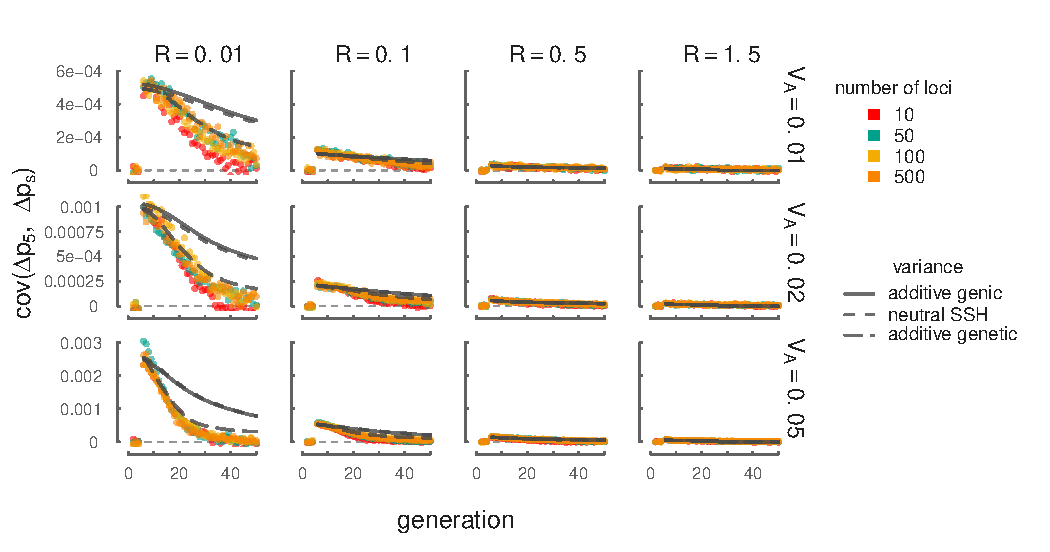
\includegraphics{./figures/sim-pred-covs-varyl-alt.pdf}

  \caption[Simulation results plotted against our theoretical expressions]{ In
    each panel the temporal autocovariance $\cov(\Delta p_5, \Delta p_s)$ is
    shown on the y-axis while generation $s$ varies along the x-axis.
    Selection is initiated on the $5^\text{th}$ generation, so $\Delta p_5$ is
    the neutral allele's frequency change across the first generation of
    selection. Each point is the temporal autocovariance between $\Delta p_5$
    and the $\Delta p_s$ in a region, averaged over 100 simulation replicates,
    with the colors indicating the number of selected loci. The gray curves
    indicate the theoretical predictions (for $L=500$ loci only) using Equation
    \eqref{eq:multilocus-triangle}, with the equation's variance provided by
    the empirically observed additive genic (solid), the additive genetic (long
    dashes), and the neutral sum of site heterozygosity approximation (short
    dashes). A thin horizontal dashed line indicates $y=0$.  Across the
    columns, the level of recombination (in Morgans) is varied; across rows,
    the initial level of additive genetic variation is varied.  Note that while
    our results here are between the frequency change at the onset of selection
    $\Delta p_5$ and some later change $\Delta p_s$, our covariance theory
    matches simulation results between any two arbitrary frequency changes
    $\Delta p_t$, and $\Delta p_s$; see Supplementary Figure
  \ref{fig:multilocus-expfit-sims-gen13}.}

  \label{fig:multilocus-expfit-sims}
\end{figure}

Figure \ref{fig:multilocus-expfit-sims} compares the fit of our theory with
differing additive genetic variances with the empirical
covariances from our multilocus simulations. In each panel, we plot the level
of temporal autocovariance between the allele frequency change across the first
two generations of selection ($\Delta p_5$) and some later allele frequency
change $\Delta p_s$ where $s$ varies along the x-axis. Each point represents
the temporal autocovariance (calculated across all sites in a region according
to Equation \ref{eq:ave-temp-autocov}) averaged across 100 replicate
simulations, with the color of the point indicating the number of selected
sites in the region. Within each panel, the temporal autocovariance predicted
by Equation \eqref{eq:multilocus-triangle} is plotted as a set of three
lines, one for each of the three different types of variance we have
substituted in for $V_a(s)$. Overall, the fit is close but varies depending on
the type of variance used for $V_a(s)$; we discuss each in turn below.

Using empirical additive genic variation (solid lines), our theory provides a
good fit to the simulation results for a short period after selection is
initiated ($\sim$5 generations) in regions with tighter linkage ($R=0.01$
Morgans) across a range of additive genetic variation parameters ($0.01 \le V_A
\le 0.05$; see Supplementary Figure \ref{fig:multilocus-expfit-sims-va-oom} for
$V_A$ varying over orders of magnitude). With looser linkage ($R \ge 0.1$
Morgans), our theory using the empirical additive genic variation fits much
more closely over a longer duration ($\sim$10-15 generations). Note that some
variability is caused by the noise of each simulation replicate around the
target initial additive genetic variation $V_a$ (see Section \ref{sec:ml-sim}),
as each replicate samples sites from a neutral coalescent. Our theory also
accurately predicts the temporal autocovariance for different choices of
reference generation, i.e.  varying $t$, see Supplementary Figure
\ref{fig:multilocus-expfit-sims-gen13}.

When we use the sum of site heterozygosity at neutral sites ($V_{a,ssh_n}$,
shown as a short-dashed lines) as a proxy for additive genic variation, the
theory fits simulations over the same timespan as using the empirical additive
genic variation. This is because (1) the SSH at neutral sites closely matches
the SSH at selected sites, and (2) both closely follow the dynamics of additive
genic variation through time (see Supplementary Figure
\ref{fig:multilocus-expfit-vark}). Using $V_{a,ssh_n}$ has the advantage that
we can directly measure neutral SSH, which proves useful later in Section
\ref{sec:meth-moments}, as we use this approach to help infer the initial
additive genic variation at the onset of selection.

Finally, we find using the additive genetic variance $V_A(s) = \var_i(z_i)$
accurately predicts the dynamics of temporal autocovariance over tens of
generations (see the long-dashed lines in Figure
\ref{fig:multilocus-expfit-sims}). Furthermore, calculating the temporal
autocovariance using the empirical additive genetic variation better fits
simulation data in regimes with tight recombination, where using genic
variation performs poorly after the first few generations (e.g. the column of
panels where $R=0.01$). Thus using the additive genetic variance in our
framework provides a good fit to the temporal dynamics over relatively long
time spans.

What differentiates $V_A(s)$ from $V_a(s)$ that could explain this better fit?
The additive genic variation $V_a(s)$ ignores the contribution of linkage
disequilibria between selected sites. We can write the additive genetic
variance as

\begin{align} V_A(s) = \var_i(z_i, s) = \underbrace{2 \alpha^2 \sum_{l=1}^L
p_{l}(s) (1-p_{l}(s))}_{\text{genic variation}, \; V_a(s)} +
\underbrace{\alpha^2 \sum_{i\ne j} D_{i,j}(s)}_\text{LD contribution }
\label{eq:var-genic-z} \end{align}
%
where $D_{i,j}(s)$ is the LD between selected sites $i$ and $j$ at time $s$.
At the onset of selection, there is no expected linkage disequilibria between
selected sites since the sites and effect sizes were randomly sampled --- in
other words, $\E(D_{i,j}(s)) = 0$. We see this in Figure
\ref{fig:multilocus-expfit-sims}, as the temporal autocovariance predicted with
$V_a(s)$ match those of $V_A(s)$ when $s = 6$ (see also Supplementary Figure
\ref{fig:multilocus-expfit-vark}, which plots the empirical additive genic and
genetic variances over time). Over time, these two quantities diverge as
negative linkage disequilibria build up. While negative linkage disequilibria
between selected sites build up due to epistasis under some forms of selection
(known as the Bulmer effect, \cite{Bulmer1971-ae,Bulmer1980-zo}), this is known
not to happen under multiplicative selection (\cite{Burger2000-an}, p. 50, 177)
that is equivalent to the exponential directional selection fitness surface we
have used in our simulations. Instead, the build up of negative linkage
disequilibria between selected sites is likely due to Hill-Robertson
interference (HRi) between selected sites \parencite{Hill1966-kd}, which
affects the total additive genetic variation that selection is acting on. HRi
refers to the creation of negative LD among beneficial alleles in finite
population resulting from the fact that beneficial alleles that are on the same
haplotype move more quickly through the population than beneficial alleles on
deleterious backgrounds, resulting in negative LD.  This negative LD among
beneficial alleles lowers $V_A$ compared to the genic $V_a$
\parencite{Hill1966-kd,Barton2005-zq,Crouch2017-xr,Good2014-yz}. In the
derivation of our expression for temporal autocovariance, we greatly simplified
the multilocus dynamics by ignoring the second term in Equation
\eqref{eq:multilocus-twopart}. This term includes the expected product of two
LD terms; each is the LD between the neutral site and a selected site. Using
full multilocus theory, one may find that by including these LD products, that
$V_A$ rather than $V_a$ factors out the expression in Equation
\eqref{eq:cov-R}, but we leave this for future work. Importantly, our
simulation results suggest that the negative linkage disequilibria created by
selective interference only affects the temporal autocovariances through the
variance term $V_a(s)$, and that the actual variance determining temporal
autocovariance is the additive genetic variance, $V_A(s)$.

In addition to modeling autocovariance through time, our theory can predict the
total temporal variance in allele frequency, $\var(p_t - p_0)$, when there is
heritable variation for fitness. Furthermore, from Equation
\eqref{eq:var-decomp} recall that we can decompose $\var(p_t - p_0)$ into
variance and covariance components. The variance components are determined by
both the magnitude of drift ($\nicefrac{1}{2N}$) and selection according to
Equation \eqref{eq:multilocus-var}, and the covariance components are
determined solely by selection according to Equation
\eqref{eq:multilocus-triangle} (assuming no inheritance of environmental
factors). Using our theory, we have predictions for each of these components
given the amount of additive genic/genetic variation for fitness, the
population size ($N$), and the amount of recombination ($R$). In Figure
\ref{fig:multilocus-expfit-cumcov}, we compare the magnitudes of these
components (averaged over the replicates of our simulations) to our theoretical
predictions. We depict the predictions for the variance and covariance
components using both the empirical additive genetic variance ($V_A$) and the
neutral sum of site heterozygosity proxy ($V_{a,ssh_n}$) as adjacent bars, each
around a point range with the point representing the average value over
simulation replicates, and the bars indicating the lower and upper quartiles
over simulations. 

\begin{figure}[!ht]
  \centering
  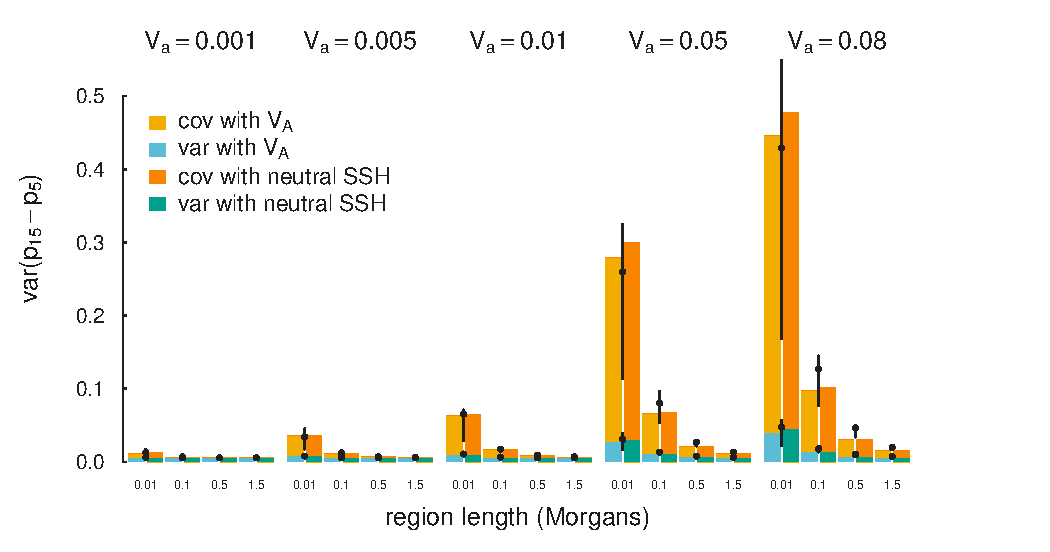
\includegraphics{./figures/cummulative-cov-var-all.pdf}

  \caption[The total contribution of temporal autocovariance to the total
  variance in allele frequency change]{Summing over generations, Equations
    \eqref{eq:multilocus-twopart} and \eqref{eq:multilocus-var-2} accurately
    predicts the total variation in allele frequency change due to variance and
    covariance components. The predicted cumulative variance in allele
    frequency change across the ten generations after selection ($\var(p_{15} -
    p_5)$) is shown as bars, using both the empirical additive genetic
    variation $V_A$ (bars to the left of the pointrange), and the empirical
    neutral sum of site heterozygosity (bars to the right of the pointrange).
    The variance and covariance components are represented by blue/green and
    orange/yellow tones respectively. Finally, we show the averaged results of
    our simulations as pointranges, with the point depicting the average and
    the bars representing the lower and upper quartiles.}
    \label{fig:multilocus-expfit-cumcov}

\end{figure}

Finally, we have found that across a wide range of recombination and additive
genetic variation parameters, the temporal autocovariance $\cov(\Delta p_t,
\Delta p_s)$ is largely determined by the compound parameter $\nicefrac{V_A}{R}$
and the number of generations between $t$ and $s$, which is a factor in
Equation \eqref{eq:ave-neut-autocov}. We show in Figure
\ref{fig:multilocus-va-r} that the temporal autocovariance $\cov(\Delta p_5,
\Delta p_s)$ from simulations across a wide range of $V_A$ and $R$ parameters
fall roughly on the same curve for each number of elapsed $s-t$ generations.


\begin{figure}[!ht]
  \centering
  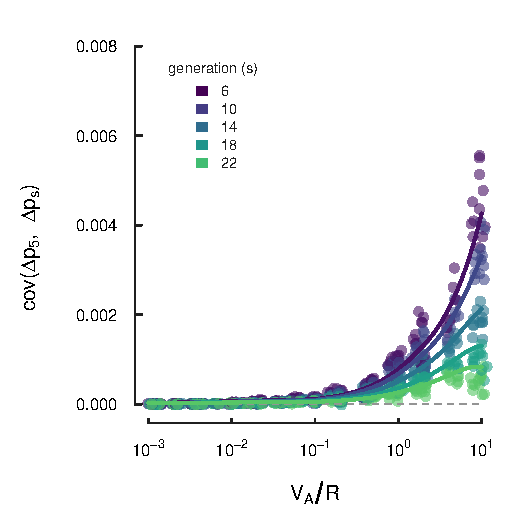
\includegraphics{./figures/va-r-cov.pdf}

  \caption[The temporal autocovariance from simualtion across a variety of
  parameters against the compound parameter $\nicefrac{V_A}{R}$]{The compound
    parameter $\nicefrac{V_A}{R}$ and the number of generations between the
    temporal autocovariance $s-t$ largely determines the magnitude of the
    temporal autocovariance across a wide spectrum of $V_A$ and $R$ parameters.
    Each point is a simulation replicate with its x-axis position given by
    $\nicefrac{V_A}{R}$, the y-axis position equal to the temporal
  autocovariance, and the number of elapsed generations ($s-t$). Each line is a
loess curve fit through each set of points for a particular generation (with
smoothing parameter $\alpha = 0.9$).}

\label{fig:multilocus-va-r}
\end{figure}

\section{Estimating linked-selection parameters from temporal autocovariance}  
\label{sec:meth-moments}

Our multilocus theory provides analytic expressions for the expected variances
and covariances of a neutral allele's frequency; thus a natural approach to
parameter estimation is to equate these expectations to averages from the data
and apply the method-of-moments. We describe a method-of-moments procedure
below to estimate the initial additive genetic variance at the onset of
selection ($V_A(1)$) in the first generation, and the drift-effective
population size ($N$) from temporal data within a single region $R$ Morgans
long, and then show a simple extension that allows this to be applied to
genome-wide data. Our basic approach is to calculate first the sample variances
and covariances of the $\tau$ observed generation-to-generation allele
frequency changes, averaging over all of the putatively neutral sites in a
region. We then equate these sample variances and covariances to our analytic
expressions for the variance and covariances, leaving us with an overdetermined
system of equations, which we solve using least squares. We demonstrate that this
simple estimation procedure provides accurate estimates of initial additive
genetic variance and the drift-effective population size. We focus on this
  procedure, as it is simple and handles  incomplete trajectories due to
  missing data or fixation/loss well. Calculating pairwise-complete covariances
  can leave sample covariances matrices non-positive definite, which makes
  maximum likelihood estimation perhaps much more difficult. Throughout, we use
  population allele frequencies (i.e.  there is no sampling noise) which
  simplifies the description of the method; in Appendix Section
  \ref{sec:sampling} we describe how the method is changed by finite sampling
  of chromosomes from a population. 

From our multilocus theory, we have analytic expressions for each element of
the $\tau \times \tau$ covariance matrix of allele frequency changes in a
region. To model the additive genic variance through time, we use the empirical
neutral sum of site heterozygosity approximation as described in Section
\ref{sec:dyn-var}. This approximates the rate that the additive genic variation
decreases through time from some initial level, $V_A(1)$, which we wish to
estimate. In total, we have $\tau + \nicefrac{\tau(\tau-1)}{2}$ unique moment
equations, which for the variance and covariance are defined as

\begin{align}
  % \E(\Delta p_t) &= 0 \\
  \frac{\var(\Delta p_t)}{\E(p_t ( 1- p_t))} \; \; &= \; \;
                                                     \frac{\widehat{V_A(1)}}{2}
                                                     \frac{\nssh(t)}{
                                                     \nssh(1)}
                                                     \mathcal{A}(R, t,t)
                                                     + \widehat{F} \;\; :=  \;\; \Sigma_{t,t}  \label{eq:mom-moments-var} \\
  \frac{\cov(\Delta p_t, \Delta p_s)}{\E(p_{t} (1-p_{t}))} \;\; &= \;\; \frac{\widehat{V_A(1)}}{2}\frac{\nssh(s)}{ \nssh(1)} \mathcal{A}(R, t,s) \;\; := \;\; \Sigma_{t,s} \; \; (\text{for} \; s > t ).
 \label{eq:mom-moments-cov}
\end{align}
%
Here the first line gives the form of $\tau$ equations for the variance of
allele  frequency changes between subsequent generations, which includes the
effect of genetic drift, $\widehat{F} =\nicefrac{1}{2N}$. The second line gives
the form of the covariances of allele frequency changes among different
generations. The term $\mathcal{A}(R, t,s)$ is the average level of linkage
disequilibrium after the $s-t$ generations that have elapsed, given there are
$R$ Morgans of recombination. In our multilocus theory section and simulations,
this is equal to the integral in Equation \eqref{eq:multilocus-triangle}.
However, we can also directly calculate a sample $\overline{\mathcal{A}(R,
t,s)}$ from observed linkage disequilibrium in a region (for details, see
Appendix Equation \eqref{eq:supp-emp-assoc}).

Following the method-of-moments, we equate each of these independent $\tau +
\nicefrac{\tau(\tau-1)}{2}$ equations for $\Sigma_{t,s}$ to the observed
sampling moments, the elements $Q_{t,s}$ of the upper triangle of the observed
heterozygosity-normalized covariance matrix $\mathbf{\widehat{Q}}$ described in
Equation \eqref{eq:ave-temp-autocov}. This yields $\tau + \nicefrac{\tau (\tau
- 1)}{2}$ equations with 2 unknown parameters: $\widehat{V_A(1)}$ and
$\widehat{N}$. We solve this overdetermined system of equations using least
squares, an approach similar to the generalized method-of-moments in
econometrics \parencite{Hansen1982-ck}. This approach finds parameter estimates
that minimize the squared error between the moment-based parameter estimate and
the true parameter value, with respect to the true parameter value. We write
the elements $Q_{t,s}$ of the upper triangle of the observed covariance matrix
in the vector $\vec{q}$, and write the method-of-moments equations as,

\begin{align}
 \vec{q} &= \widehat{V_A(1)} \vec{a} + \widehat{F} \vec{b} + \vec{\varepsilon}  
 \label{eq:mom-regression} 
\end{align}
where the elements of $\vec{a}$  and $\vec{b}$, in the same order as $\vec{q}$, are given by
\begin{align}
  a_{t,s} &= \frac{1}{2}\frac{\nssh(s)}{\nssh(t)}\mathcal{A}(R, t,s),~ b_{t,s} = \delta_{t,s}
\end{align}
%
where $\delta_{t,s}$ is an indicator variable that is $1$ when $s=t$
and zero otherwise.

Then, we can readily estimate the parameters $\widehat{V_A(1)}$ and
$\widehat{F}$ using least squares. We then obtain an estimate of $\widehat{N}$
by taking $\nicefrac{1}{2\widehat{F}}$. Since these equations are not
statistically independent, we cannot assume $\cov(\vec{\varepsilon}) = \sigma^2
\mathbf{I}$. However, this does not affect our estimates $\widehat{V_A(1)}$ and
$\widehat{F}$, as the least squares procedure is unbiased regardless of the
covariance structure between the error terms \parencite[p.
26]{Christensen2011-cg}.


Using this method-of-moments approach, we sought to infer the parameters of 20
of the replicates across the 254 parameter combinations (the same as used in
Figure \ref{fig:multilocus-expfit-sims}). We use the first five generations
after the onset of selection to infer $\widehat{V_A(1)}$ and $\widehat{N}$, as
for this short timespan the additive genetic variance is well approximated
using sum of neutral site heterozygosity approach (see Section
\ref{sec:ml-sim-res}). Each simulation replicate includes around 500 neutral
sites (the exact number is random, see Appendix \ref{sec:supp-ml-sim-param} for
details).

Applying our approach to these simulations, we find we can infer both the
initial level of additive genetic variation $V_A(1)$, and the effective
population size $N$ from multilocus temporal data. In Figure
\ref{fig:mom-fits-both}A, we show that our method-of-moments gives reasonable
estimates for the initial level of additive genetic variance over orders of
magnitude of additive genetic variation, and different recombination regimes.
As additive genetic variation for fitness becomes weaker (the left side of the
figure), our estimates become more noisy. In Figure \ref{fig:mom-fits-both}B we
show the simultaneously estimated population size $N$ against the true
population size value. We also plot the estimated $N_e$ (not accounting for
selection) from a simple temporal estimator, $N_e = -t / (2 \log(1-F))$
\parencite{Krimbas1971-et,Waples1989-sj} where $F$ is Wright's standardized
variance \parencite{Wright1931-fl}. While with high $V_A$ and low $R$, the
method-of-moments approach still underestimates $N$, it performs far better
than a standard temporal $N_e$ estimator that does not account for selection.
In Appendix Figure \ref{fig:mom-fits-both-finite}, we include a version of this
figure calculated using the method of moments on sample allele frequencies for
a sample of size $n=100$ chromosomes.

\begin{figure}
  \centering
  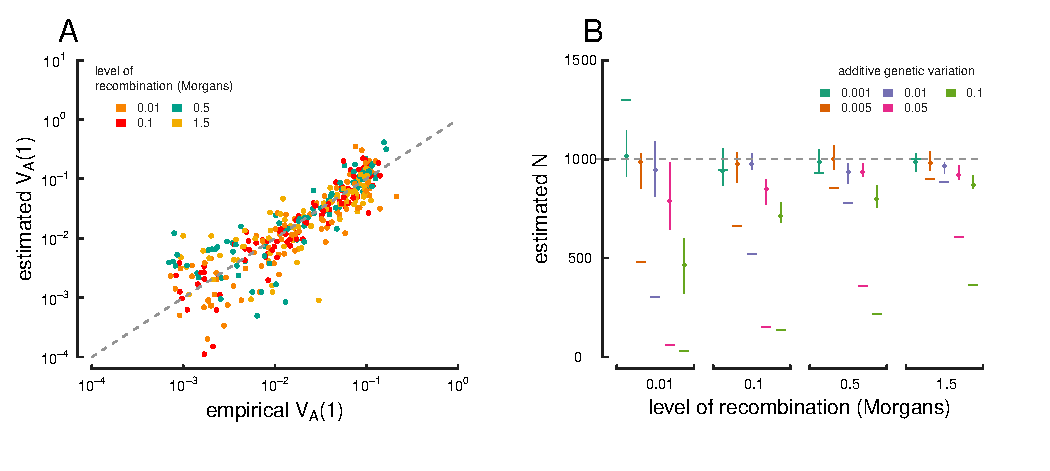
\includegraphics{./figures/mom-fits-both-alt.pdf} 

  \caption[Method of moment estimates of $V_A$ and $N$ against their true
  values from simulation data]{True parameter values and estimates using the method-of-moments
    approach on multilocus simulation data. (A) The true $V_A(1)$ (x-axis) and
    $\widehat{V_A(1)}$ estimated from the variance/covariance matrix (y-axis)
    for each simulation replicate across different levels of recombination
    (indicated by each point's color). The dashed gray line shows the $y=x$
    line where an estimate is exactly true to its real value. Note that the
    plot is on a log-log scale, as $V_A$ varies across orders of magnitude in
    our simulations. (B) Estimated drift-effective population size
    ($\widehat{N}$) across a range of simulations with different levels of
    additive genetic variance and recombination. Each point denotes the median,
    with lines denoting the interquartile range. A simple temporal estimate of
    the effective population size, estimated accounting for the effects of
    selection, is averaged for each replicate and plotted as a dash.  The true
    value ($N = 1,000$) is shown with the dashed gray line. Population
    frequencies (without sampling noise) are used in this figure; see Appendix
  Figure \ref{fig:mom-fits-both-finite} for an analogous figure calculated with
sample frequencies.}

\label{fig:mom-fits-both}
\end{figure}

We can extend this approach to whole-genome data by imagining partitioning 
the genome into $B$ non-overlapping windows of length $w_{\textrm{BP}}$ in
basepairs (e.g. megabase windows). We first assume that windows contribute
uniformly to the genome-wide level of additive genetic variance for  fitness,
and show how our method-of-moments approach can be used to estimate a global
$V_A(1)$. Assuming a uniform distribution of genetic variance across basepairs,
the total additive variance is $V_A(1) = v_A(1) B w_{\text{BP}}$, across our B
windows, where $v_A(1)$ is the additive genetic variance per basepair. As each
window $i$ contributes to $v_A(1) w_{\text{BP}}$, our least squares approach
given by Equation \eqref{eq:mom-regression} becomes

\begin{align}
  \Sigma_{t,s,i} &= \frac{\widehat{V_A(1)}}{2} \frac{1}{B} \frac{SSH_n(s)}{SSH_n(1)} \mathcal{A} (R_i, t,s ) +
            \widehat{F} \delta_{t,s}+ \varepsilon, \;\;  \text{for} \; s \geq t.
            \label{eq:mom-windows}
\end{align}

However, we expect \emph{a priori} that windows containing more coding bases
might disproportionately contribute to the total additive genetic variance.
This suggests an alternative model to fit where partitions of the additive
genetic variance across windows are proportional to the number of coding bases,
similar to background selection and other linked selection models
\parencite{Rockman2010-bw,McVicker2009-ax,Corbett-Detig2015-gt}. Thus, we could
write total $V_A(1) = v_A(1) \sum_{i=1}^B w_{\text{CBP},i}$ where
$w_{\text{CBP},i}$ is the number of coding or exonic basepairs in window $i$
(this could be any quantifiable annotation feature in the window), and
$W_\text{CBP} = \sum_{i=1}^B w_{\textrm{BP}},i$ is the total number of coding
bases in the genome. With window $i$ contributing $v_A(1) w_{\text{CBP}, i}$ to the
additive genetic variance and having map length $R_i$, we now define $\vec{q}$,
$\vec{a}$, and $\vec{b}$ as having elements given by the equations

\begin{align} 
  \Sigma_{t,s,i} &= \frac{\widehat{V_A(1)}}{2} \frac{w_{\text{CBP},i} \; SSH_n(s)}{W_{\text{CBP}} \; SSH_n(1)} \mathcal{A} (R_i, t, s) + \widehat{F} \delta_{t,s} + \varepsilon, \;\; \text{for} \; s \ge t.
  \label{eq:mom-windows-cbp}
\end{align}
%
Again, the parameters of this model, $\widehat{V_A(1)}$ and $\widehat{N}$, can
be estimated with least squares. When analyzing genome-wide data, these various
models could potentially be compared to an out-of-sample procedure, using
inferred parameters to estimate the mean-squared predictive error between the
two models for the remaining windows \parencite{Elyashiv2016-vt}. The
confidence intervals for our method-of-moments estimates could be obtained
through bootstrapping genomic windows since the errors are not identically and
independently distributed.

%One can resample (with replacement) the underlying putatively neutral loci,
%and then recalculate the empirical variance and covariance matrix.  Note that
%since least squares is being used here as an estimation procedure and not a
%model of the data, AIC and other model comparison techniques are not
%appropriate.  With these resampled empirical variance and covariances, then
%one can re-estimate the parameters using the method moments. In cases where
%genomic windows vary in their mapping coverage, we suggest replacing the
%least-squares estimation procedure with weighted least squares where weights
%are determined by the proportion of covered bases in a window.

\subsection{Estimating the proportion of variance in frequency change due to linked selection}

We can also estimate what fraction of allele frequency change over $t$
generations ($\nicefrac{\var(p_t - p_0)}{t}$) is due to linked selection acting
to perturb the frequency trajectories of neutral alleles. We have developed two
approaches: first, a more conservative approach that considers only the
contribution of selection to the temporal autocovariance, and second, a more
exact approach that uses the estimated effective population size to include the
contribution of selection to both variances and covariances of allele frequency
change.

\begin{figure}
  \centering
  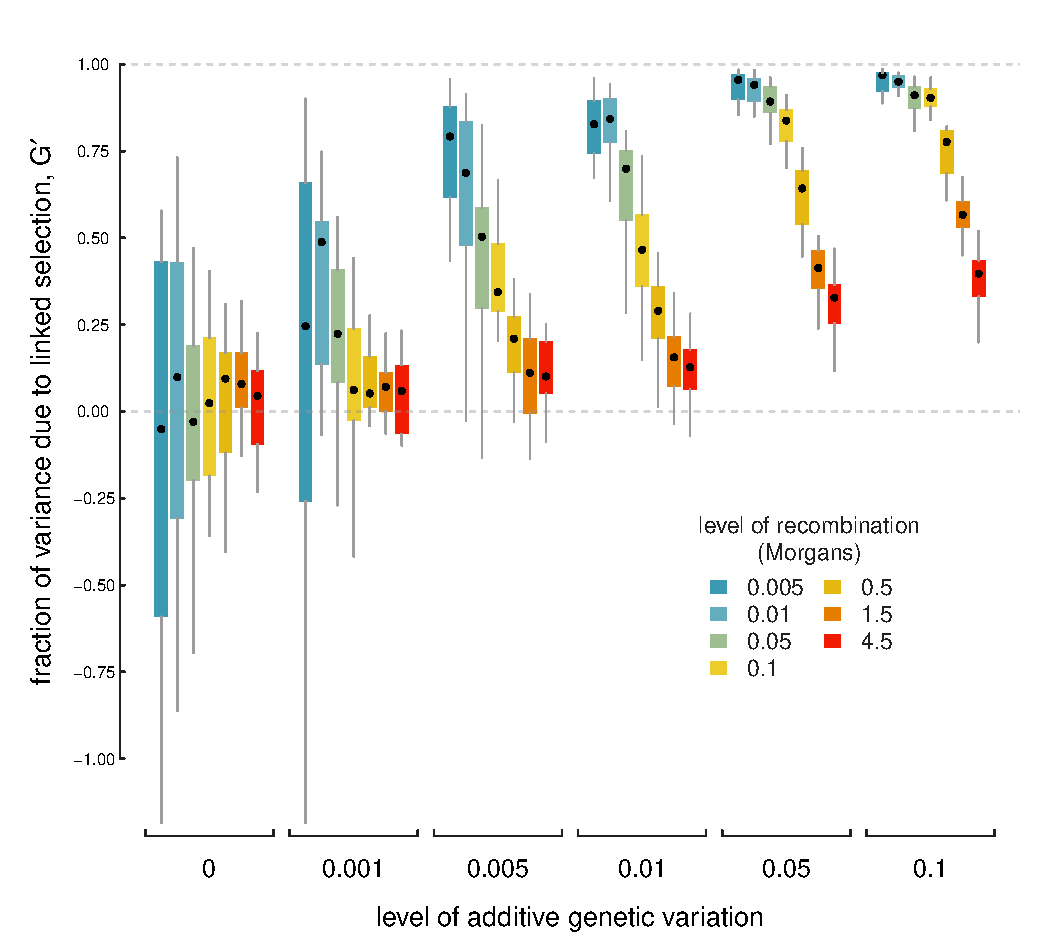
\includegraphics{./figures/estimate-gp.pdf} 

  \caption[The proportion of total allele frequency change due to linked
  selection from simulation results, for a variety of parameters]{The
    proportion of total variance in allele frequency changes caused by linked
    selection, $G'$, across a variety of different levels of additive genetic
    variance (each group of boxplots), and different levels of recombination
    (each colored boxplot within a group). Each boxplot shows the spread of
    values across 20 replicates, with $\widehat{N}$ being calculated across
  each replicate.} 

  \label{fig:est-g}
\end{figure}

First, a simple estimate of the total fraction of the variance in allele
frequency change ($G$) caused by linked selection is

\begin{align}
  \label{eq:g-def}
  G = \frac{\sum_{t \ne s}\cov(\Delta p_t, \Delta p_s)}{\var(p_t - p_0)}.
\end{align}

However, this estimator is conservative because it ignores the contribution
that linked selection has on the variance in allele frequency change across a
single generation (the $\var(\Delta_{_H} p_t)$ term in Equation
\ref{eq:var-decomp-1}). If we include these variance terms, we have a
less-conservative estimator we call $G'$,

\begin{align}
  G' &= \frac{\sum_{t \ne s}\cov(\Delta p_t, \Delta p_s) + \sum_{i=1}^t \var(\Delta_{_H} p_i)}{\var(p_t - p_0)} \nonumber \\
     &= 1 - \frac{\sum_{i=1}^t \var(\Delta_{_M} p_i) + \sum_{i=1}^t \var( \Delta_{_N} p_i)}{\var(p_t - p_0)}.
  \label{eq:g-prime}
\end{align}

We can think of the numerator of the second term in Equation \eqref{eq:g-prime}
as the variance in allele frequency change in a Wright--Fisher population
without selection.  Recall that under a Wright--Fisher model, the standardized
variance across $t$ generations is approximately $(1 - \exp(-\nicefrac{t}{2N}))
\approx p_0(1-p_0) \times \nicefrac{t}{2N}$, where this second approximation
works for short time spans ($\nicefrac{t}{2N} \ll 1$).  This suggests that we
can use our method-of-moments estimate of the effective population size without
the effects of selection, $\widehat{N}$, and compare the fraction of
standardized variance we expect under this rate of drift to the empirical
standardized variance,

\begin{align}
  G' &= 1 - \frac{t \E(p_{0}(1-p_{0})) }{2 \widehat{N} \var(p_{t} - p_{0}) }.
\end{align}

Figure \ref{fig:est-g} shows the estimated $G'$ from the method-of-moment
$\widehat{N}$ estimates using 20 replicates of simulated data. We learn
three important points about our $G'$ estimator. First, for low $V_A$, or $V_A
= 0$, the estimator is quite noisy. Second, although the signal can be noisy
for low $V_A$, the relationship between $G'$ and level of recombination is
consistent with selection affecting the total variance in allele frequency
changes across the genome. Finally, this suggests that a negative relationship
between $G'$ and recombination rate, calculated in windows across the genome,
is a robust signal of linked selection impacting the total variance in allele
frequency change. Furthermore, we would expect a positive relationship between
the number of coding basepairs per window (when such information is available)
and $G'$, which could serve as another robust signal of linked selection
impacting the total variance in allele frequency change.

\subsection{Fluctuating Selection}
\label{sec:fluct-sel}

Thus far we have assumed that fitness effect sizes are constant through time,
that is $\alpha_{t,l} =  \alpha_{s,l}$, for all $t, s$. In natural populations,
changes in the environment or composition of the population may cause these
effect sizes to change through time, due to changing selection pressures and
changes in the epistatic environment experienced by alleles. If these changes
occur within the timeframe of recorded allele frequency changes, the levels of
temporal autocovariance will differ from the levels predicted from our
directional selection theory. However, from Equation
\eqref{eq:multilocus-twopart} we can see that the magnitude of temporal
autocovariance is determined in large part by $\E(\alpha_t \alpha_s)$.

Here, we discuss how temporal autocovariance behaves under an example of strong
fluctuating selection: when selection on a trait changes direction at some
point. Specifically, we change the fitness function $w(z_i) = e^{z_i}$ to
$w(z_i) = e^{-z_i}$ after some timepoint $t^*$; this is equivalent to changing
$\alpha_{s,l} = - \alpha_{t,l}$ iff $s \ge t^*$, and $\alpha_{s,l} =
\alpha_{t,l}$ otherwise for all other $s < t^*$.

When such a strong change in the direction of selection occurs, the temporal
autocovariance between timepoints before and after the change becomes negative,
since temporal autocovariance is determined by the product $\alpha_{t}
\alpha_{s}$ for $t \ne s$ (here we are holding effects constant across loci).
We have validated this using the same simulation procedure as described in
Section \ref{sec:ml-sim}, except on generation 15 we reverse the direction of
selection on the trait by changing the fitness function $w(z) = e^z$ to $w(z) =
e^{-z}$. In Figure \ref{fig:fluct-sel}A, we show the temporal autocovariance
$\cov(\Delta p_5, \Delta p_s)$ for varying $s$ along the x-axis (in this case,
$V_a=0.05$, $R=0.1$, and $L=500$). During the first five generations, the
temporal autocovariance behaves as it does under directional selection,
decaying due to the decrease in additive genetic variance and the breakdown of
linkage disequilibrium. Then, on the $15^\text{th}$ generation, the direction
of selection on the trait with breeding value $z_i$ reverses and temporal
autocovariance becomes negative since $\alpha_{s,l} \alpha_{t,l} < 0$ for all
$s \ge t^*$ and $t < t^*$. Under this simple flip in the direction of selection
pressure, the genic variance, $V_a(s) = 2 \alpha^2 \sum_l p_{s,l}(1-p_{s,l})$,
in the expressions for the temporal autocovariance can be replaced with $V_a(s)
= 2 \alpha_s \alpha_t \sum_l p_{s,l}(1-p_{s,l})$, akin to a genetic/genic
covariance.  In Figure \ref{fig:fluct-sel}A, the gray line is our predicted
level of temporal autocovariance proportional to $V_A \mathcal{A}(R,t, s)$
given by Equation \eqref{eq:multilocus-cov-sum} before generation 15, and after
generation it is proportional to $-V_A \mathcal{A}(R,t, s)$ (using the
empirical additive genetic variance).  Note, however, that the dynamics of
additive genetic variance under fluctuating selection are more complex than
under directional selection.  Whereas under directional selection the genetic
variance decays as selection proceeds, under fluctuating selection there can be
a transient increase in the additive genetic variance (seen in Figure
\ref{fig:fluct-sel}A between generations 15-24).  This transient inflation
of the additive genetic variance is caused by the increase in the
heterozygosity of haplotypes that had experienced reduced heterozygosity due to
directional selection. With the direction of selection reversed, previously
selected haplotypes move to more intermediate frequencies, which increases the
additive genetic variance until selection proceeds and this variance decays
(generations 25 and onwards).  Overall, the dynamics of additive genetic
variance under fluctuating selection are more complicated than under
directional selection which makes inference using our sum of site
heterozygosity approximation infeasible.


\begin{figure} \centering 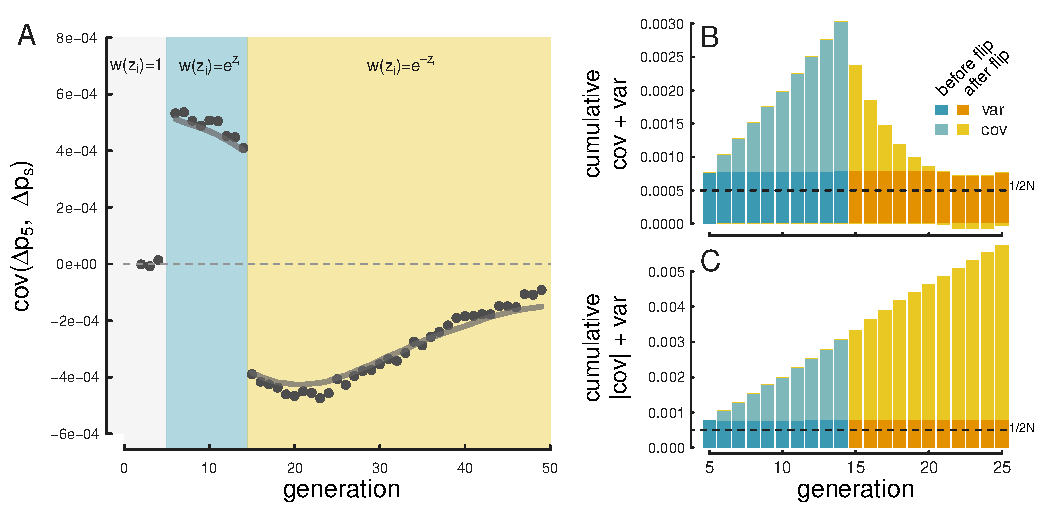
\includegraphics{./figures/fluct-sel.pdf}
  \caption[The impact of fluctuating selection on temporal autocovariance and
  $G$]{A: The covariance $\cov(\Delta p_5, \Delta p_s)$, where $s$ is varied
    on the x-axis, for $V_a=0.05$, $R=0.1$, and $L=500$ averaged over 100
    replicates. Selection begins in generation 5 (with the fitness function
    $w(z_i)=e^{z_i}$) and on generation 15 the direction of selection flips
    (and the fitness function becomes $w(z_i) = e^{-z_i}$). The gray line shows
    our directional selection temporal autocovariance prediction modified so
    that after the flip in the direction the trait is selected, we plot the
    \emph{negative} theoretical level of temporal autocovariance. B: The
    average cumulative variance and covariances through the generations for the
    same simulation parameters, with the height of the bar representing the
    total cumulative variation $\var(p_t - p_0)/t$. Since the direction of
    selection flips, the covariances terms after generation 15 become negative,
    leading the total variance to decrease (the negative covariances are
    plotted below the x-axis line). After generation 21, the total covariance
    is negative, leading the total variance to dip below the level of variance
    alone (determined by drift and heritable fitness variation). The dark gray
    dashed line shows the level of variance expected by drift alone
    ($\nicefrac{\var(p_t-p_0)}{t} = \nicefrac{1}{2N}$). C: The effect of using
  the absolute value of covariance, which prevents the negative autocovariances
from canceling out the effects of other covariances before the direction of
selection changed.} \label{fig:fluct-sel} \end{figure}


Since fluctuating selection can create \emph{negative} temporal autocovariance,
the total amount of autocovariance over time (e.g. $\sum_{t\ne s} \cov(\Delta
p_t, \Delta p_s)$) can misrepresent the actual amount that linked selection is
affecting allele frequencies on shorter timescales. This, in turn, leads our
estimator $G$, for the fraction of variance in allele frequency due to linked
selection, to underestimate the total contribution of linked selection to
variation in allele frequencies over the time period.  We show an example of
this in Figure \ref{fig:fluct-sel}B, which depicts the total variance in
allele frequency change $\nicefrac{\var(p_t - p_0)}{t}$ through time,
partitioned into variance and covariance components and colored according to
whether the generation was before and after the reverse in directional
selection. The covariances $\sum_{t\ne s} \cov(\Delta p_t, \Delta p_s)$
increase as they would under directional selection, but after generation 15,
the contribution of covariance begins to decrease as negative autocovariances
accumulate. By generation 20, the total covariance terms have a net negative
effect, and actually act to decrease the total variance $\nicefrac{\var(p_t -
p_0)}{t}$ for a few generations below the constant level expected under drift
and heritable variation.

To more fully capture the contribution of selection allele frequency change, we
modify $G$, using the absolute value of the covariances, 

\begin{align}
  \label{eq:g-abs}
  G_{abs} = \frac{\sum_{t \ne s}|\cov(\Delta p_t, \Delta p_s)|}{\var(p_t - p_0)}
\end{align}
%

which prevents negative temporal autocovariances from canceling out the effects
of positive temporal autocovariances, since both are a reflection of linked
selection acting on neutral allele frequency changes. We show $G_{abs}$ in
Figure \ref{fig:fluct-sel}C, where even after the change in the directional
selection we see a steady accumulation of covariance contributing to total
variance $\nicefrac{\var(p_t - p_0)}{t}$. This also suggests one plausible way
to check for genomically wide-spread fluctuating selection would be to test if
$G_{abs} > G$. However, we note that in contrast to our simulations, it is
likely that in natural populations only a subset of alleles change their
relationship to fitness. This may act to dampen the magnitude of, but not
completely reverse the direction of genome-wide temporal autocovariance, and so
different approaches may be needed to identify fluctuations.

\section{Discussion}

Currently, the prevailing empirical approach to studying linked selection
relies on using samples from a single timepoint and modeling the patterns of
diversity subject to different functional constraints and in different
recombination environments. The early theoretical work underpinning empirical
analyses of linked selection's effects on diversity were primarily full sweep,
recurrent hitchhiking models, where beneficial mutations arise in the
population and then sweep to fixation
\parencite{Maynard_Smith1974-lc,Stephan1992-jc,Kaplan1989-ld}. Furthermore, by
looking at the patterns of diversity around amino acid substitutions or the
site frequency spectrum in low recombination regions, researchers have teased
apart the effects of background selection and hitchhiking in \emph{Drosophila}
\parencite{Begun2007-bg,Elyashiv2016-vt}, humans
\parencite{Hernandez2011-gs,McVicker2009-ax}, and some plants species
\parencite{Nordborg2005-vt,Beissinger2016-cm,Schmid2005-on,Williamson2014-oy}.
Yet, as other theoretical models of hitchhiking incorporating changes in the
environment \parencite{Kopp2007-mc,Kopp2009-lo,Kopp2009-pj}, sweeps originating
from standing variation \parencite{Hermisson2005-hs}, and multiple competing
beneficial haplotypes \parencite{Pennings2006-lj} have been developed, it has
become rather more difficult to detect the signal of these hitchhiking
phenomenon in empirical data. We have proposed here that temporal autocovariance
offers a unique and measurable signal of linked selection over shorter
timescales that provides a fuller picture of the ways in which genome-wide
diversity has affected by these other hitchhiking phenomena. 

\subsection{Empirical Applications and Future Directions}

Here, we've developed expressions for temporal variances and autocovariances,
and applied these to model temporal variances and covariances during
directional selection on a trait. We have demonstrated how one can (1) estimate
the additive genetic variance for fitness and the drift-effective population
size, (2) estimate the fraction of variance in allele frequency change due to
linked selection, and (3) evaluate whether fluctuating selection is operating
from these temporal variances and autocovariances. However we recognize a
series of limitations and difficulties when applying these methods to empirical
data and natural populations.

First, one difficulty with temporal sampling of natural populations is the risk
that the genetic composition may change drastically due to migration or biased
sampling across timepoints. Since our theory assumes a constant-sized and
isolated population, migration into the sampled population presents a serious
potential confounder. For example, seasonal migration could create an influx of
new alleles that could at best dampen signals of directional selection across
seasons, or at worst create a signal of artificial covariance between like
seasons. Similar biases could occur if a sampling method incidentally preferred
certain subgroups in a stratified population. This could occur, for example, if
individuals differ in some behavior affecting their likelihood of being sampled
across different temporal environments, which could cause spurious covariances.
While such sampling issues and migration might be able to be detected
\emph{post hoc} from exploratory data analysis approaches like PCA, studying
isolated natural populations and carefully designing sampling schemes would
lead to the best inference. Importantly, the effects of gene flow and other
temporal inhomogeneities could differ across recombination environments, as
among population differentiation will be more pronounced in regions of low
recombination and high functional density
\parencite{Keinan2010-ry,Burri2017-ml,Nachman2012-sw}. In situations where
  migration is a factor, one way forward might be to study the contribution of
  linked selection after partitioning out the effects of gene flow across
  recombinational and functional environments by extending admixture inference
approaches that estimate the genome-wide effect of drift and admixture.

Second, our method-of-moments approach relies on assuming we can approximate
the dynamics of the decay of the additive genetic variance that was present
at a reference timepoint by using the observed changes in sum of site
heterozygosity in a region as a proxy for its decay. While we have shown this
model works under directional selection in a relatively idealized setting,
inference in natural populations may be complicated by changes in the
environment that induce the effect sizes across loci to vary across timepoints.
While our fluctuating selection results show that our directional selection
theory extends to changes in the direction of selection with minor adjustments
(e.g. Figure \ref{fig:fluct-sel}), having the effect sizes vary across each
generation would complicate the dynamics of additive genetic variance through
time and make inference of $V_A$ difficult.  Similarly, we assume that effect
sizes are constant across sites. Variance in effect sizes across a region will
not bias our results unless there is covariance between effect size and local
recombination rate. Further work is required to develop statistical methods to
test for violations of our assumptions about effect sizes remaining constant
across time, and to potentially incorporate these complications into inference.

Along similar lines, we have focused on directional selection under a
multiplicative model. However, selection experiments, a natural place to apply
our method, often use truncation selection, which generates systematic
epistasis for fitness and thus linkage disequilibria among loci
\parencite{Burger2000-an,Walsh2018-bt}. Similarly, in natural populations
stabilizing selection will act on many traits, which can also generate LD among
loci. These selective processes will act to rapidly reduce the additive genetic
variance for fitness across time, especially in low recombination regions, and
to reduce the initial additive genetic variance in low recombination regions.
Simulating the effect of truncation selection and stabilizing selection on
temporal covariances in allele frequencies seems a useful direction. Our model
may prove to be a useful null model of selection that the complications of
epistasis and different dynamics of the additive genetic variance could be
tested against. 

Finally, while we demonstrate that our method-of-moments estimation approach is
simple and leads to unbiased estimators, we see opportunities for simple
extensions and other inference procedures. Differences in recombination rates
and coding density are relatively easily accommodated (Equation
\ref{eq:mom-windows-cbp}). In fitting our model we assumed a parametric form to
the initial LD between neutral and selected loci; however, in practice the
initial linkage disequilibria between neutral polymorphisms and putatively
functional sites could be estimated empirically. Using the empirical LDs in
Equation \eqref{eq:mom-windows-cbp} could make the inference somewhat analogous
to LD Score regression \parencite{Bulik-Sullivan2015-ls}. The LD Score of a SNP
is simply the sum of the $R^2$'s of the focal SNP to all SNPs within some large
physical genomic window, which could be used in place of the integral in
Equation \eqref{eq:multilocus-triangle}. Using this equation, $V_A$ could be
estimated by regressing the temporal covariance of a SNP on its LD Score. An
alternate approach would be to use likelihood methods to model each neutral
site's frequency changes using the set of pairwise linkage disequilibria and
recombination distances between the neutral site and all neighboring
polymorphic sites. Then, genome-wide or region-wide estimates could be found
via composite likelihood methods, in a similar manner to
\textcite{McVicker2009-ax} and \textcite{Elyashiv2016-vt}. Furthermore, one
could include different $V_A$ parameters for neighboring polymorphic sites with
specific functional annotations, such as those in genic regions, introns,
exons, etc. to see how different classes of sites contribute to the additive
genetic variance for fitness. Our hope is that statistical methods to quantify
the effects of linked selection over short timescales will improve and be
combined with measures of phenotypic change, leading to a more synthetic view
of how selection on ecological timescales occurs at the genetic and phenotypic
levels.

As the number of empirical temporal genomic studies continue to increase, it is
worth mentioning how our study of temporal autocovariance suggests a few ways
to optimize experimental design to increase the power to differentiate the
effects of selection from drift. First, one should ideally sample frequencies
from consecutive generations for at least some timepoints during the duration
of the experiment. This is because the variance in allele frequency change
$\var(\Delta p_t)$ between adjacent generations is only impacted by the
heritable variance in offspring number, $\var(\Delta_{_H} p_t)$ (see Equation
\ref{eq:var-decomp-1}), and not by the accumulation of temporal autocovariance
terms (e.g. Equation \ref{eq:var-decomp}); this allows for more accurate
estimates of $G$. In cases where a long study duration is needed but sequencing
is limited to only a subset of generations, a mixed duration sampling design,
such as sampling generations 1 through 4, and then 10 through 14, and so forth
could serve as a compromise. Second, as described in Appendix Section
\ref{sec:sampling}, the shared sampling noise between adjacent timepoints
creates a negative bias in autocovariance that must be corrected for. As
described in Equations \eqref{eq:corrected-var} and \eqref{eq:corrected-cov},
we can estimate this bias from data, but this introduces additional uncertainty
into our parameter estimates. In cases where the experimenter suspects \emph{a
priori} that fluctuating selection is occurring, e.g. between two seasons, we
recommend at least two temporal samples per season. This allows one to
differentiate negative covariance occurring from the bias correction procedure
underestimating bias from negative covariance caused by fluctuating selection
through comparing non-adjacent timepoints that differ in season. Finally, once
can directly remove the effects of the technical sampling noise created by
variation in sequencing by dividing up temporal samples and barcoding them into
two groups (e.g. A and B). Then, the sample covariance estimate $\cov(\Delta
p_{t,A}, p_{s,B})$ does not share the technical sampling noise, reducing the
bias (but note some bias remains due to the sampling process where individuals
are sampled from the population.)

\subsection{Connecting Temporal Linked Selection with Single Timepoint Studies}

Our goal in this paper is to suggest that quantifying variance and
autocovariance using temporal data sets can help us understand the impact
linked selection has across the genome on short timescales, which supplements
our current view informed mainly by single timepoint studies. A range of
approaches to estimate the parameters and impact of models of linked selection
from a single contemporary timepoint have been developed
\parencite{Wiehe1993-ja,Begun1992-ey,Sella2009-rf,Elyashiv2016-vt,McVicker2009-ax,Hudson1994-yq}.
These estimates necessarily reflect linked selection over tens to hundreds of
thousands of generations. One question is whether these estimates of the
proportion of allele frequency change due to linked selection should line up
with those over shorter time periods? Some forms of linked selection may be
fairly uniform over time, whereas rare, strong sweeps will have a huge impact
on long-term patterns of variation but may be hard to catch in temporal data.
Conversely, as we discuss below, fluctuating selection may lead to stronger
signals of linked selection on short timescales than seen in long-term
snapshots.

Studies of contemporary data have revealed multiple lines of evidence for the
effect of linked selection in a variety of taxa. If linked selection is
pervasive across the genome, diversity could be severely dampened as most sites
would be in the vicinity of selected sites, thus reducing the genome-wide level
of diversity without leaving strong local signals differentiated from the
background. This is one proposed resolution of Lewontin's paradox, the
observation that diversity levels occupy a narrow range across taxa with
population sizes that vary by orders of magnitude
\parencite{Lewontin1974-jb,Maynard_Smith1974-lc,Gillespie2001-ll,Leffler2012-zj}.
\textcite{Elyashiv2016-vt} estimated a $77$ - $89\%$ reduction in neutral
diversity due to selection on linked sites in \emph{Drosophila melanogaster},
and concluded that no genomic window was entirely free of the effect of
selection. Similarly, \textcite{Corbett-Detig2015-gt} has found evidence of a
stronger relative reduction in polymorphism due to linked selection in taxa
with larger population sizes. However, these reductions fall short of the many
orders of magnitude required for linked selection to explain Lewontin's paradox
\parencite{Coop2016-gx}.   


One limitation of these approaches is that they require estimating $\pi_0$, the
level of diversity in the absence of linked selection, usually from the
diversity in high-recombination regions with low gene content. The average
genome-wide reduction of diversity can then be judged relative to $\pi_0$.
Ideally, $\pi_0$ would be a measure of the average diversity due entirely to
drift and demographic history, i.e. unaffected by heritable fitness variation.
However, there are two complications with this. First, as
\textcite{Robertson1961-ho} first showed, even a site completely unlinked from
sites creating heritable fitness variation experiences a reduced effective
population size due to the total additive genetic variance for fitness at these
unlinked sites, and thus lower diversity (see also \cite{Santiago1995-hx}). The
second complication is that if linked selection is sufficiently strong, the
bases used to measure $\pi_0$ may not be sufficiently unlinked from
fitness-determining sites to plateau to the \textcite{Robertson1961-ho} level
of diversity, a known potential limitation
\parencite{Coop2016-gx,Elyashiv2016-vt}. Overall, the empirical studies relying
on present-day samples from a single timepoint could be underestimating the
effects pervasive linked selection has on diversity. If linked selection can be
observed over suitable timescales in temporal data, we might be able to
disentangle some of these effects. For example, if high recombination regions
still show temporal autocovariance in allele frequency change, we would have
evidence that even these regions are not free of the effect of linked selection
and we might be able to estimate its long term impact on levels of diversity. 

Temporally or spatially fluctuating selection has long been discussed as an
explanation for abundant, rapid phenotypic adaptation over short timescales,
yet over longer timescales both phenotypic changes and molecular evolution
between taxa are slow \parencite{Messer2016-mn,Hendry1999-zu,Gingerich1983-cc}.
However, most of our approaches to population genomic data are built on simple
models with constant selection pressures, as typically we have not had the data
to move beyond these models \parencite{Messer2016-mn}. Currently, many
approaches to quantify the impact of linked selection due to hitchhiking assume
classic sweeps, where a consistent selection pressure ends in the fixation of a
beneficial allele \parencite{Sella2009-rf,Hernandez2011-gs,Wiehe1993-ja}.
However, fluctuating selection can have a larger effect on reducing diversity
than classic sweeps \parencite{Barton2000-zg} depending on the timescales over
which such fluctuations occur. In fact as \textcite{Barton2000-zg} points out,
the total effect of classic Maynard-Smith and Haigh-type sweeps on diversity is
limited by the relatively slow rate of substitutions. We show that when the
direction of selection on a trait abruptly reverses, this creates negative
autocovariance between the allele frequency changes before and after the
reverse in direction. We can observe the shift by plotting autocovariances over
time and noting when they become negative, indicating a negative additive
genetic covariance between fitness at two timepoints. Here we assume a simple
form of fluctuating selection: where selection pressures on all of our sites
flip at some timepoint. In reality, selection pressures will change on only
some traits, and some of the genetic response will be constrained by
pleiotropy, thus only some proportion of the additive genetic variance will
change. Still, we expect some level of negative covariance after a reversal in
the direction of selection, and there is additional signal of fluctuating
selection by comparing how the strength of temporal autocovariance varies with
recombination and the initial level of linkage disequilibrium in the genome.

\subsection{Connecting Estimates of $V_A$ from Temporal Genomic Data and
Quantitative Genetic Studies}

The temporal covariance of allele frequencies potentially offers a way to
estimate the additive genetic variance for fitness, as illustrated by our
method-of-moments approach across genomic windows. The additive genetic
variance for fitness can, like any other trait, be estimated through
quantitative genetics methods, which exploit the phenotypic resemblance between
relatives and their known kinship coefficients
(\cite{Kruuk2004-zk,Shaw2013-rx}; see \cite{Hendry2018-se} for a review), and
these methods have been applied to estimate the additive genetic variance for
fitness from natural populations \parencite{Burt1995-dd,Mousseau1987-uy,}.
Ideally, one could reconcile quantitative genetic measures of fitness variance
with estimates from allele frequency covariance. For example,
\textcite{Charlesworth2015-am} undertook a similar analysis in \emph{Drosophila
melanogaster}, comparing population genetic estimates of fitness variance to
quantitative genetics estimates, highlighting a discordance potentially
consistent with undetected large-effect alleles that are likely maintained by
some form of balancing selection. By allowing us to directly measure fitness
variation from population genetic data over very short timescales, temporal
data could help untangle the causes of this discordance. A natural extension of
this would be to see which regions contain the greatest inferred levels of
additive genetic variance for fitness, and test for functional covariates such
as the number of coding bases, etc. Whereas previous temporal studies have
focused on finding loci under selection, inferring the level of additive
genetic variance could provide a more complete view of how much selection
operates over short timescales.

\subsection{Concluding Thoughts}

With temporal data we can directly partition the total variance in allele
frequency change across generations, $\var(p_t-p_0)$ into components according
to the underlying process governing their dynamics: drift and linked selection.
Since the trajectory of a neutrally drifting polymorphism does not autocovary,
evidence of temporal autocovariance across neutral sites in a closed population
is consistent with linked selection perturbing these sites' trajectories. If we
consider drift to be the process by which non-heritable variation in
reproductive success and Mendelian segregation cause allele frequencies to
change, then this is estimable from and separable from the effects of linked
selection using temporal data. This helps frame the long-running debate about
the roles neutral drift and linked selection have in allele frequency dynamics
into a problem that can potentially be directly quantified by the contribution
of each distinct process with temporal data.

\section{Code and Data Availability}

All code and simulation data to reproduce these results are available on GitHub
at \url{https://github.com/vsbuffalo/tempautocov}.


%\bibliographystyle{chicago}

\newpage


%\appendix

\section{Appendix} 
\counterwithin{figure}{section}
\setcounter{figure}{0}    

\begin{singlespacing}

\begin{table}[!htbp]
  \caption[Table of Notation]{Notation}
  \begin{tabular}{r|p{12cm}}
 Symbol & Usage  \\ \hline
 $p_t$ & Allele frequency in generation/timepoint $t$  \\
 $\Delta p_t$ & Allele frequency change between generations $t+1$ and $t$, $\Delta p_t = p_{t+1} - p_t$ \\
 $\Delta_{_N} p_t $ & Frequency change due to non-heritable variation in fitness, \eqref{eq:delp-decomp}, \eqref{eq:var-decomp-1}  \\
 $\Delta_{_M} p_t $ & Frequency change due to Mendelian segregation, \eqref{eq:delp-decomp}, \eqref{eq:var-decomp-1} \\
 $\Delta_{_H} p_t $ & Frequency change due to heritable differences, \eqref{eq:delp-decomp}, \eqref{eq:var-decomp-1} \\
 $N$ & Census population size of breeding individuals \\
 $N_e$ & Effect population size \\
 $f_i$ & Fitness (expected number of offspring) of individual $i$, \eqref{eq:ap-freq}\\
 $\alpha_{t,l}$ & Effect size in generation $t$ and locus $l$, \eqref{eq:neut-change}, \eqref{eq:ap-delta-H} \\
 $L$ & Total number of loci impacting fitness, \eqref{eq:neut-change} \\
 $g_{i,l} \in \{0, 1, 2\}$ & Individual $i$'s gene count at locus $l$, \eqref{eq:ap-delta-H-2} \\
 $x_{i} \in \{0, 1, 2\}$ & Individual $i$'s neutral gene count at the tracked neutral site, \eqref{eq:neut-change}, \eqref{eq:ap-delta-H-2}, \eqref{eq:ap-delta-H-3} \\
 $D_{t,l}$ or $D_{t,l}'$ & \hangindent=1em Gametic linkage disequilibrium between the tracked neutral site and selected locus $l$ at time $t$, Supplementary Figure \ref{fig:ld-cartoon}, \eqref{eq:neut-change}, \eqref{eq:ap-delta-H-2}, \eqref{eq:ap-delta-H-3} \\
 $D_{t,l}''$ & \hangindent=1em Non-gametic disequilibrium between the tracked neutral site and selected locus $l$ at time $t$, Supplementary Figure \ref{fig:ld-cartoon}, \eqref{eq:neut-change}, \eqref{eq:ap-delta-H-2}, \eqref{eq:ap-delta-H-3} \\
 $\E(\mathcal{R}_{t,l}^2)$ & \hangindent=1em The squared correlation coefficient of linkage disequilibrium between the tracked neutral site and selected site $l$ at time $t$, \eqref{eq:cov-R}, \eqref{eq:ap-D}\\
 $r_l$ & \hangindent=1em The recombination fraction between the tracked neutral site and selected site $l$\\
 $V_a(s)$ & The additive genic variance, \eqref{eq:multilocus-cov-sum} \\ 
 $V_A(s)$ & The additive genetic variance, \eqref{eq:var-genic-z} \\ 
 $R$ & The total level of recombination in the region, in Morgans, \eqref{eq:ave-neut-autocov} and Figure \ref{fig:cartoon} \\ 
 $r(g)$ & \hangindent=1em A mapping function (i.e. Haldane's), which maps a position $g$ to a recombination fraction.\\ 
 $\rho$ & The population recombination rate, $\rho = 4Nr$, Section \ref{sec:temp-autocov-aveneut} \\ 
 $\mathcal{A}(R, t, s)$ & \hangindent=1em The average linkage disequilibrium in a region of $R$ Morgans, that persisted from generation $t$ to generation $s$, \eqref{eq:multilocus-triangle} \\
 $V_N$ & The non-heritable variance in offspring number, \eqref{eq:multilocus-var} \\
 $SSH(t)$ & The sum of site heterozygosity at selected sites time $t$, \eqref{eq:VA-SSH} \\
 $SSH_n(t)$ & The sum of site heterozygosity at neutral sites at time $t$, \eqref{eq:VA-SSH} \\
 $ssh_n(t)$ & \hangindent=1em The proportion of sum of site heterozygosity at neutral sites at time $t$ relative to $SSH(1)$, $SSH_n(t) / SSH_n(1)$ \eqref{eq:VA-ssh} \\
 $z_i$ & \hangindent=1em The breeding value of the trait that determines fitness, $z_i = \sum_{i=1}^L \alpha g_{i,l}$, see appendix section \ref{ap:multilocus} \\
 $w(z_i)$ & The fitness of individual $i$ with fitness function $w(\cdot)$, see appendix section \ref{ap:multilocus} \\
\end{tabular}
\end{table}

\end{singlespacing}

\begin{singlespacing}

\begin{table}[!htbp]
  \setcounter{table}{0}
  \caption[Table of Notation, continued]{Notation, continued}
  \begin{tabular}{r|p{12cm}}
 Symbol & Usage  \\ \hline
 $\mathbf{Q}$ & The sample standardized variance-covariance matrix, \eqref{eq:ave-temp-autocov} \\
 $Q_{t,s}$ & The elements of the observed sample matrix $\mathbf{Q}$, \eqref{eq:ave-temp-autocov} \\
 $\mathbf{\Sigma}$ & \hangindent=1em The standardized variance-covariance matrix, based on our theoretical expressions \\
 $\Sigma_{t,s}$ & The elements of the standardized variance-covariance matrix, \eqref{eq:multilocus-triangle}, \eqref{eq:multilocus-var} \\
 $\Delta p_{n,t}$ & \hangindent=1em The allele frequency change at site $n$ between times time $t+1$ and $t$, \eqref{eq:ave-temp-autocov} \\
 $\tau$ & \hangindent=1em The number of allele frequency changes observed, e.g. after sampling for $\tau + 1$ timepoints \\
 $V_{a,ssh_n}(t)$ & \hangindent=1em The additive genic variation at time $s$ as approximated by the observed decay in the sum of site heterozygosity at neutral sites, \eqref{eq:VA-ssh} \\
 $\var_i(z_i)$ & The variance in trait values taken over individuals, \eqref{eq:var-genic-z} \\
 $\widehat{V_A(1)}$ & \hangindent=1em The method-of-moments estimate of the additive genetic variance in the first generation, \eqref{eq:mom-moments-cov}, \eqref{eq:mom-moments-var} \\
 $\widehat{F}$ & \hangindent=1em The method-of-moments estimate of Wright's standardized variance, $F = \nicefrac{1}{2N}$, \eqref{eq:mom-moments-cov}, \eqref{eq:mom-moments-var} \\
 $\widehat{N}$ & \hangindent=1em The method-of-moments estimate of drift-effective population size, $N = \nicefrac{1}{2F}$ \\
 $\sigma^2$ & \hangindent=1em The sampling noise around each element of the sample variance-covariance matrix. \\
 %$\vec{a}, \; \vec{b}$ & Vectors of the 
 $B$ & The total number of windows after partitioning the genome, \eqref{eq:mom-windows} \\
 $w_{text{BP}}$ & Width of windows (in basepairs), \eqref{eq:mom-windows} \\
 $v_A(1)$ & The average additive genetic variance per basepair \\
 $w_{\text{CBP}}$ & Number of coding basepairs in a window, \eqref{eq:mom-windows} \\
 $W_{\text{CBP}}$ & Total number of coding basepairs in the genome, \eqref{eq:mom-windows-cbp}  \\
   $G$ & \hangindent=1em A conservative measure of the total variance in allele frequency change due to linked selection, \eqref{eq:g-def} \\
   $G'$ & \hangindent=1em An alterate, less conservative measure of the total variance in allele frequnecy change due to linked selection, \eqref{eq:g-prime} \\
   $G_{abs}$ & A variant of $G$ using the absolute value of covariances, \eqref{eq:g-abs} \\
\end{tabular}
\end{table}

\end{singlespacing}

\subsection{Decomposition of Allele Frequency Change}
\label{ap:decomp}

This decomposition of \emph{neutral} allele frequency change between two
consecutive generations is based on that of \textcite{Santiago1995-hx}. We
imagine a closed Wright--Fisher population of $N$ diploids, where each diploid
$i$ contributes $k_i \sim \text{Multinom}(\nicefrac{f_i}{N}, 2N)$ gametes to
the next generation. We assume that the population size is constant, such that one
diploid begets one diploid and thus $\E_i(f_i) = 1$. The neutral allele
frequency in the next generation can be thought of as each of the $N$ parents
passing their average genotype $\nicefrac{x_i}{2}$ (where $x_i \in\{0, 1, 2\}$
is the number of tracked neutral alleles individual $i$ carries) to their $k_i$
gametes, plus a random Mendelian deviation $b_{ij} \in \{0, -\nicefrac{1}{2},
\nicefrac{1}{2}\}$ to each offspring $j$. Then, the frequency in the next
generation can be written as

\begin{align}
  p_1 &= \frac{1}{N} \sum_{i=1}^N \left(k_i \frac{x_i}{2} + \sum_{j=1}^{k_i} b_{ij} \right)
  \label{eq:ap-freq}
\end{align}
%
where $b_{ij} = \delta_{x_i, 1} (\nicefrac{1}{2} - B_j)$, $B_j \sim
\text{Bernoulli}(\nicefrac{1}{2})$ and $\delta_{x_i, 1}$ is an indicator
function that is one when the individual $i$ is a heterozygote (i.e. $x_i=1$),
and zero otherwise.

If we further decompose the number of offspring of individual $i$ into the
genetic and non-genetic contributions, $k_i = f_i + d_i$, then

\begin{align}
  p_1 &= \frac{1}{N} \sum_{i=1}^N \left( (f_i + d_i) \frac{x_i}{2} + \sum_{j=1}^{k_i} b_{ij} \right) \nonumber \\
      &= \frac{1}{2N} \sum_{i=1}^N f_i x_i + \frac{1}{2N} \sum_{i=1}^N d_i x_i + \frac{1}{N} \sum_{i=1}^N  \sum_{j=1}^{k_i} b_{ij} 
\end{align}
%
and the change of the neutral allele's frequency is the difference $\Delta p = p_1 - p_0$ where $p_0 = \nicefrac{1}{2N} \sum_{i=1}^{N} x_i$. Then,

\begin{align}
\Delta p = p_1 - p_0 &= \frac{1}{2N} \sum_{i=1}^N f_i x_i + \frac{1}{2N} \sum_{i=1}^N d_i x_i + \frac{1}{N} \sum_{i=1}^N  \sum_{j=1}^{k_i} b_{ij} - \frac{1}{2N} \sum_{i=1}^N x_i \nonumber \\
                     &= \underbrace{\frac{1}{2N}\sum_{i=1}^N x_i (f_i - 1)}_{\Delta_{_H} p_1} + \underbrace{\frac{1}{2N} \sum_{i=1}^N d_i x_i}_{\Delta_{_N} p_1} + \underbrace{\frac{1}{N} \sum_{i=1}^N \sum_{j=1}^{k_i} b_{ij}}_{\Delta_{_M} p_1}.
\end{align}
%

These $d$'s broadly capture non-heritable variation in an individual's
offspring number, with $\E[d_i]=0$. In a quantitative genetics framework
$\var_i(d_i)$ can include non-genetic variation in the lifetime reproductive
success of individuals ($V_E$), in population genetic models $\var_i(d_i)$ can
accommodate the sampling of parents to form the next generation, e.g.
multinomial sampling of individuals from fitnesses \parencite{Santiago1995-hx}.
From now forwards, we assume that variation in these $d$'s is non-heritable. We
note that in non-panmictic populations, chance covariances could be created
between a neutral polymorphism and environmental component of their phenotype,
especially as a population expands its range into new environments that affect
the phenotype, and variants ``surf'' to higher frequencies
\parencite{Edmonds2004-xf,Hallatschek2008-mn,Excoffier2008-ep}.

Note that by construction, the allele frequency change components $\Delta_{_N}
p_t$ $\Delta_{_M} p_t$, and $\Delta_{_H} p_t$ are orthogonal within each
individual, given the neutral allele frequency $x$. Partitioning the allele
frequency change for an individual $i$ into its components,

\begin{align}
  \Delta p_{t,i} &= \underbrace{\frac{1}{2} x_i (f_i - 1)}_{\Delta_{_H} p_{t,i}} + 
       \underbrace{\frac{1}{2} x_i d_i}_{\Delta_{_N} p_{t,i}} + 
       \underbrace{\delta_{x_i,1}(\nicefrac{k_i}{2} - M(k_i))}_{\Delta_{_M} p_{t,i}} \\
       &= \frac{1}{2} x_i (f_i - 1) + 
       \frac{1}{2} x_i d_i + 
       \delta_{x_i,1}(\nicefrac{f_i}{2} - M(f_i)) + 
       \delta_{x_i,1}(\nicefrac{d_i}{2} - M(d_i))
\end{align}
%
where $M(n) = \sum_{j=1}^{n} B_j \sim \text{Binom}(n, \nicefrac{1}{2})$.

Two random variables $X, Y$ are uncorrelated if $\cov(X, Y) = \E(XY)
- \E(X)\E(Y)= 0$, and are orthogonal if either has an expected value of zero
such that $\E(XY) = 0$. We show briefly that taking expectations \emph{over
conceptual evolutionary replicates}, the terms are orthogonal. First, the terms
$x(f-1)$ and $x d$ are orthogonal (dropping $i$ subscripts),

\begin{align}
  \nicefrac{1}{4} \cov(x(f-1), x d) &= \nicefrac{1}{4}(\E(x^2 d (f-1)) - \E(x(f-1)) \E(x d)) \nonumber \\
                                    &= \nicefrac{1}{4} (\E(x^2) \E(d) \E(f-1) - \E(x)\E(f-1) \E(x d)) \nonumber \\
                                    &= 0
\end{align}
%
since $\E(f) = 1$ across evolutionary replicates due to the assumption that
population size is constant, and $x \perp f$, as across all evolutionary
replicates, there is no dependence between a particular neutral allele an
individual carries and their fitness (though in particular replicates, such
associations occur). Similarly, for the case $x=1$ (other cases are all zero,
and can be ignored), it can be shown using the law of total expectation that
$\cov(x d, \nicefrac{d}{2} - M(d)) = 0$ (and likewise with $x (f-1)$ and
$\nicefrac{f}{2} - M(f)$). Note that across individuals within a population,
there are weak covariances in their number of offspring as the total number of
offspring must sum to $N$; under a Multinomial offspring distribution, these
are of order $\nicefrac{1}{N}$.


\subsection{Temporal variance and autocovariance under multilocus selection}
\label{ap:multilocus}

We assume the phenotype of an individual $i$ has an additive polygenic basis,
such that their breeding value is $z_i = \sum_{l=1}^L \alpha_{t,l} g_{i,l}$
which deviates around a mean of zero, and $\alpha_{t,l}$ is the additive effect
size at locus $l$ in generation $t$, and $g_{i,l} \in \{0,1,2\}$ is individual
$i$'s allele count at this locus (note that effect of non-heritable
environmental noise affecting the trait is accounted for in the $d_i$ terms
above). We impose directional selection on this trait using an exponential
fitness function, such that individual $i$'s fitness is $f_i =
\nicefrac{w(z_i)}{\bar{w}} \approx e^{z_i}$ (assuming $\bar{w} \approx 1$). If
we assume individuals' phenotypic values do not deviate too far from their mean
value of zero, we can approximate $f_i$ as: $f_i \approx 1 + \sum_{l=1}^L
\alpha_{t,l} g_{i,l}$. Then, we can write the change in neutral allele
frequency due to only heritable variation in fitness ($\Delta_{_H} p_t$) as a
covariance between fitness and the neutral allele frequency across individuals
in generation $t$, 

\begin{align}
  \Delta_{_H} p_t &= \frac{1}{2N} \sum_{i=1}^N x_i \left(f_i - 1\right) \\
                  &= \frac{1}{2} \cov_i(x_i, f_i) \\
                  &= \frac{1}{2} \cov_i(x_i, \sum_{l=1}^L \alpha_{t,l} g_{i,l})
  \label{eq:ap-delta-H}
\end{align}
%
which is the is the Robertson-Price covariance
\parencite{Price1970-si,Robertson1966-fs,Lynch1998-wl,Walsh2018-bt}.

Now, we break up the genotypic value $x_i$ into the contributions of each of
the two gametes that formed individual $i$, $x_i = x_i' + x_i''$, and likewise
with the trait locus $g_{i,l} = g_{i,l}' + g_{i,l}''$, where $x_i', x_i'',
g_i',$ and $g_i''$ are all indicator variables. Expanding out the covariances, we have

\begin{align}
  \label{eq:ap-delta-H-2}
  \Delta_{_H} p_t &= \frac{1}{2}\cov(x_i' + x_i'', \sum_{l=1}^L \alpha_{t,l} (g_{i,l}' + g_{i,l}'')) \nonumber \\
                &= \frac{1}{2}\left(\cov(x_i', \sum_{l=1}^L \alpha_{t,l} (g_{i,l}' + g_{i,l}'')) + \cov(x_i'', \sum_{l=1}^L \alpha_{t,l} (g_{i,l}' + g_{i,l}'')) \right) \nonumber \\ 
  % &= \cov(x_i', \sum_{l=1}^L \alpha_{t,l} g_{i,l}' + \sum_{l=1}^L \alpha_{t,l} g_{i,l}'') + \cov(x_i'', \sum_{l=1}^L \alpha_{t,l} g_{i,l}' + \sum_{l=1}^L \alpha_{t,l} g_{i,l}'') \\
                &= \frac{1}{2} \left( \cov(x_i', \sum_{l=1}^L \alpha_{t,l} g_{i,l}') + \cov(x_i', \sum_{l=1}^L \alpha_{t,l} g_{i,l}'') + \cov(x_i'', \sum_{l=1}^L \alpha_{t,l} g_{i,l}') + \cov(x_i'', \sum_{l=1}^L \alpha_{t,l} g_{i,l}'') \right).
\end{align}

Each of these covariances is between the neutral allele and a selected allele,
either on the same gamete (either maternal or paternal) or across gametes.
These covariances can be written as linkage disequilibrium terms,

\begin{align} \Delta_{_H} p_t &= \frac{1}{2} \left( \cov(x_i', \sum_{l=1}^L
  \alpha_{t,l} g_{i,l}') + \cov(x_i', \sum_{l=1}^L \alpha_{t,l} g_{i,l}'') +
\cov(x_i'', \sum_{l=1}^L \alpha_{t,l} g_{i,l}') + \cov(x_i'', \sum_{l=1}^L
\alpha_{t,l} g_{i,l}'') \right) \nonumber \\ &= \frac{1}{2} \left( \sum_{l=1}^L
\alpha_{t,l} \cov(x_i', g_{i,l}') + \sum_{l=1}^L \alpha_{t,l} \cov(x_i',
g_{i,l}'') + \sum_{l=1}^L \alpha_{t,l} \cov(x_i'',  g_{i,l}') + \sum_{l=1}^L
\alpha_{t,l} \cov(x_i'',  g_{i,l}'') \right) \nonumber \\ &= \frac{1}{2} \left(
\sum_{l=1}^L \alpha_{t,l} D_{l}' + \sum_{l=1}^L \alpha_{t,l} D_{l}'' +
\sum_{l=1}^L \alpha_{t,l} D_l'' + \sum_{l=1}^L \alpha_{t,l} D_l' \right)
\nonumber \\ &=  \sum_{l=1}^L \alpha_{t,l} D_{l}' + \sum_{l=1}^L \alpha_{t,l}
D_{l}'' \label{eq:ap-delta-H-3} \end{align}
%
where $D_L'$ is the linkage disequilibrium between alleles on the same gamete
(the gametic LD), and the $D_l''$ is the across-gamete LD (non-gametic LD); see
\textcite{Weir1996-mv}, p. 121. This equation also appears in
\textcite{Kirkpatrick2002-aw} (eqn. 10).

We ignore non-gametic linkage disequilibria $D_l''$ as these are weak under
random mating, and write the multilocus temporal covariance between the allele
frequency changes $\Delta p_t$ and $\Delta p_s$ as

\begin{align}
  \cov(\Delta p_t, \Delta p_s) &=  \E(\Delta p_t \Delta p_s)  - \E(\Delta p_t) \E (\Delta p_s) \nonumber \\
                               &=  \E \left(\sum_{l=1}^L \alpha_{t,l} D_{t,l}' \sum_{l=1}^L \alpha_{s,l} D_{s,l}' \right) \nonumber \\
                               &=  \underbrace{\sum_{l=1}^L \alpha_{t,l} \alpha_{s,l}\E(D_{t,l}'  D_{s,l}')}_{\text{persistence of association to selected site} \; l}  \; + 
  \underbrace{\sum_{l \ne k} \alpha_{t,k} \alpha_{s,l}\E(D_{t,k}'  D_{s,l}')}_{\text{cross-associations between two selected sites} \; k \; \text{and} \; l} \label{eq:app-multilocus-twopart}
\end{align}
%
since $\E(\Delta p_t) = 0$. 

\paragraph{Modeling the dynamics of LD between selected and neutral sites}
\label{ap:hh-ld}

Here, we outline a model of the changes in linkage disequilibria between the
focal neutral site and selected sites, which allows us to derive an expression
for the first term in Equation \eqref{eq:app-multilocus-twopart}. Typically,
models of multilocus selection track the genetic changes in a population by
transforming between a representation of haplotype frequencies to a
representation of allele frequencies, linkage disequilibria, and higher-order
linkage disequilibria
\parencite{Barton1987-gl,Barton1991-pw,Turelli1988-wi,Turelli1990-kd}. We for
the moment avoid the difficulty of a full multilocus treatment by assuming that
the linkage between selected sites is loose enough that one selected site's
frequency change is independent of the change at other selected sites, e.g.
there is no selective interference; this was an assumption in past treatments
(\cite{Santiago1995-hx,Santiago1998-bs}; see \cite{Barton2000-zg} for
discussion of this). Specifically, we model the dynamics of the LD between the
neutral site and each selected site as they would behave under a single sweep
model.

We adapt Barton's (\citeyear{Barton2000-zg}) model for LD dynamics during a
sweep. We imagine a polymorphic neutral locus has alleles $B_1$ and $B_2$ with
frequencies $p$ and $1-p$. We partition the allele frequency of $B_1$ by
conditioning on which allele at the selected site (either $A_1$ or $A_2$) is
carried on the same background, e.g. $P(B_1 | A_1)$, and $P(B_1 | A_2)$, such
that $P(B_1) = P(B_1 | A_1) P(A_1) + P(B_1 | A_2) P(A_2)$. Then, the linkage
disequilibrium between neutral and selected sites can be expressed as $D =
P(A_1) P(A_2) (P(B_1|A_1) - P(B_1|A_2)))$. To simplify notation, we denote the
frequency of the neutral allele on the different fitness backgrounds at time
$t$ by $P(B_1 | A_1) = p^{(1)}_{t}$ and $P(B_1 | A_2) = p^{(2)}_{t}$ and the
selected allele at locus $l$ frequency as $p_{t,l}$, we have the LD between the
focal neutral site and selected site $l$ at time $t$ is

\begin{align}
  D_{t,l} &= p_{t,l} (1-p_{t,l}) ( p^{(1)}_{t} - p^{(2)}_{t} ).
\end{align}

% \begin{align}
%   D &= P(A_1 B_1) - P(A_1) P(B_1) \\
%     &= P(B_1 | A_1) P(A_1) - P(A_1) P(B_1) \\
%     &= P(A_1) (P(B_1 | A_1) - P(B_1)) \\
%     &= P(A_1) (P(B_1 | A_1) - (P(B_1|A_1) P(A_1) + P(B_1|A_2) P(A_2))) \\
%     &= P(A_1) P(A_2) (P(B_1|A_1) - P(B_1|A_2))) \\
% \end{align}

Selection changes the frequency $p_{t,l}$ through time, and recombination acts
to disassociate the neutral allele with its backgrounds. The expected
difference $p^{(1)}_{t} - p^{(2)}_{t}$ is maintained with probability
$(1-r_{l})$ each generation \parencite{Barton2000-zg}. If the initial
generation is $t$ and the future generation is $s$ ($s > t$), and $r_{l}$ is
the recombination rate between the focal neutral locus and selected site $l$,
this leads to

\begin{align}
  ( p^{(1)}_{s} - p^{(2)}_{s} ) = ( p^{(1)}_{t} - p^{(2)}_{t} ) (1-r_{l})^{s-t}.
\end{align}
%
Then, we can use this to describe the dynamics of $D_{s,l}$ to generation $t$,

\begin{align}
  \frac{p_{s,l} (1-p_{s,l})}{p_{s,l} (1-p_{s,l})}( p_{s}^{(1)} - p_{s}^{(2)} ) &= \frac{p_{t,l} (1-p_{t,l})}{p_{t,l} (1-p_{t,l})}( p_{t}^{(1)} - p_{t}^{(2)} ) (1-r)^{s-t} \nonumber \\
  \frac{D_{s,l}}{p_{s,l} (1-p_{s,l})} &= \frac{D_{t,l}}{p_{t,l} (1-p_{t,l})} (1-r)^{s-t} \nonumber \\
  D_{s,l} &= D_{t,l}\frac{ p_{s,l} (1-p_{s,l})}{p_{t,l} (1-p_{t,l})} (1-r_{l})^{s-t}
  \label{eq:ld-dyn}
\end{align}
%
(c.f. \cite{Stephan2006-xz}, equations (30) and (31)). Now, we can find the
expected product $\E(D_{t,l} D_{s,l})$ by multiplying both sides by $D_{t,l}$
and taking expectations. We treat the allele frequency trajectory as
deterministic, giving us,

\begin{align}
  D_{t,l} D_{s,l} &= D_{t,l}^2\frac{ p_{s,l} (1-p_{s,l})}{p_{t,l} (1-p_{t,l})} (1-r_{l})^{s-t} \nonumber \\
  \E(D_{t,l} D_{s,l}) &= \E(D_{t,l}^2)\frac{ p_{s,l} (1-p_{s,l})}{p_{t,l} (1-p_{t,l})} (1-r_{l})^{s-t}.
\end{align}
%
Then, we simplify this by replacing $\E(D_{t,l}^2)$ with
$\E(\mathcal{R}_{t,l}^2) p_{t,l}(1-p_{t,l}) p_{t}(1-p_{t})$ (where
$\E(\mathcal{R}_{t,l})$ is the square of the correlation between the neutral
site and selected site $l$ at time $t$; \cite{Hill1968-ue}),

\begin{align}
  \E(D_{t,l} D_{s,l}) &= \E(D_{t,l}^2)\frac{ p_{s,l} (1-p_{s,l})}{p_{t,l} (1-p_{t,l})} (1-r_{l})^{s-t} \nonumber \\
                      &= \E(\mathcal{R}_{t,l}^2) p_{t} (1-p_{t}) p_{t,l} (1-p_{t,l}) \frac{ p_{s,l} (1-p_{s,l})}{p_{t,l} (1-p_{t,l})} (1-r_{l})^{s-t} \nonumber \\
                      &= \E(\mathcal{R}_{t,l}^2) p_{t} (1-p_{t}) p_{s,l} (1-p_{s,l}) (1-r_{l})^{s-t}.
  \label{eq:ap-D}
\end{align}
%
Returning to Equation \eqref{eq:app-multilocus-twopart} and replacing the
$\E(D_{t,l} D_{s,l})$ terms with our expression above, 

\begin{align}
  \cov(\Delta p_t, \Delta p_s) &= \sum_{l=1}^L \alpha_{t,l} \alpha_{s,l}
  \E(\mathcal{R}_{t,l}^2) p_{t} (1-p_{t}) p_{s,l} (1-p_{s,l}) (1-r_{l})^{s-t} 
\end{align}
%
again ignoring the  cross-associations between selected sites.  Dividing our
temporal covariance by the neutral site's $p_t(1-p_t)$, we can write the
multilocus temporal covariance in a standardized form (analogous to Wright's
F),

\begin{align}
  \frac{\cov(\Delta p_t, \Delta p_s)}{p_t(1-p_t) } &=
  \sum_{l=1}^L \alpha_{t,l} \alpha_{s,l} p_{s,l} (1-p_{s,l}) \E(\mathcal{R}_{t,l}^2) (1-r_l)^{s-t}.
  \label{eq:basic-multilocus-sum}
\end{align}

\paragraph{Using average additive genetic variation}
\label{ap:ml-ave-Va}

We can approximate Equation \eqref{eq:basic-multilocus-sum} by noticing that
the terms $\alpha_{t,l} \alpha_{s,l} p_{s,l} (1-p_{s,l})$ are similar to an
additive genic variation if effect sizes remain constant through time. We make
that assumption here, writing $\alpha_l := \alpha_{t,l} = \alpha_{s,l}$, leading to

\begin{align}
  \frac{\cov(\Delta p_t, \Delta p_s)}{p_t(1-p_t) } &=
  \sum_{l=1}^L \alpha_{l}^2 p_{s,l} (1-p_{s,l}) \E(\mathcal{R}_{t,l}^2) (1-r_l)^{s-t}.
  \label{eq:basic-multilocus-sum-2}
\end{align}
%
We can further simplify this by assuming that there is no covariance between
the additive genic variation at a selected site, and the LD between that
selected site and the neutral site. We write the additive genic variation at
site $l$ at time $s$ as $v_{a,l}(s) = 2 \alpha_l^2 p_{s,l}(1-p_{s,l})$, and the
average additive genic variation across loci as $\overline{v_{a}(s)} := \nicefrac{V_a(s)}{L} =
\frac{1}{L} \sum_l 2 \alpha_l^2 p_{s,l}(1-p_{s,l})$. Then, each locus's
additive genic variation can be expressed as: $v_{a,l}(s) = \overline{v_a(s)} +
\varepsilon_l$. Substituting this, the autocovariance is 

\begin{align}
  \frac{\cov(\Delta p_t, \Delta p_s)}{p_t(1-p_t) } &= \frac{1}{2} \sum_{l=1}^L v_{a,l(s)} \E(\mathcal{R}_{t,l}^2) (1-r_l)^{s-t}  \nonumber \\
                                                   &= \frac{1}{2} \sum_{l=1}^L (\overline{v_a(s)} + \varepsilon_l) \E(\mathcal{R}_{t,l}^2) (1-r_l)^{s-t} \nonumber  \\
                                                   &= \frac{1}{2}\underbrace{\overline{v_{a(s)}}}_{\substack{\text{average genic}\\ \text{variation per locus}}} \times \underbrace{\left(\sum_{l=1}^L \E(\mathcal{R}_{t,l}^2) (1-r_l)^{s-t}\right)}_\text{sum of persistence associations}  + \frac{1}{2} \underbrace{\left(\sum_{l=1}^L \varepsilon_l \E(\mathcal{R}_{t,l}^2) (1-r_l)^{s-t}\right)}_\text{effect-association covariation}.
\end{align}
%
We assume that this last term, which is non-zero in expectation only if there
is covariance between the additive genic variation at a selected site and the
expected LD between the selected and the neutral sites is zero. Rewriting the
total genic variation as $V_a(s)$,

\begin{align}
  \frac{\cov(\Delta p_t, \Delta p_s)}{p_t(1-p_t)} &= \frac{V_a(s)}{2L} \sum_{l=1}^L \E(\mathcal{R}_{t,l}^2) (1-r_l)^{s-t}.
\end{align}

\paragraph{Continuous approximation to chromosomes}
\label{ap:ml-cont}

Currently, we have treated the positions of the selected sites are fixed,
conditioning on knowing that a selected site $l$ has a recombination fraction
$r_l$ away from the focal neutral site site. Here, we make a few further
assumptions. First, we assume the $L$ selected loci are each independently and
identically uniformly distributed along a \emph{continuous} region of $R$
Morgans in length ($g \sim U(-\nicefrac{R}{2}, \nicefrac{R}{2})$), and we now
calculate the covariance at a focal neutral site at the origin by taking
expectations over the random positions of these sites. Second, we assume that
the LD between the neutral and selected site $l$ only depends on the
recombination fraction between the sites. Since $g$ is the genetic distance,
the recombination fraction is now provided by a mapping function $r(g)$ that
maps genetic distances to recombination fractions.  Throughout the paper and in
the simulations, we use Haldane's mapping function, $r(g) = \frac{1}{2} (1 -
e^{-2|g|})$ (note the absolute value translates positions on
$[-\nicefrac{R}{2}, \nicefrac{R}{2}]$ to distances to the focal neutral site).
Next, we assume the LD between two sites can be completely determined by the
distance between the focal neutral site and a random selected site, allowing us
to rewrite $\E(\mathcal{R}^2_{t,l})$ as the function
$\E(\mathcal{R}^2_t(r(g)))$. Now, letting $\E_{r_l}(\cdot)$ represent the
expectation taken over the random positions of selected sites on the genetic
map, 

\begin{subequations}
  \begin{align}
    \frac{\cov(\Delta p_t, \Delta p_s)}{p_t(1-p_t) } &= \frac{V_a(s)}{2L} \sum_{l=1}^L \E_{r_l} \left( \E(\mathcal{R}_{t}^2(r_l)) (1-r_l)^{s-t} \right) \label{eq:cont-approx-step-1} \\
                                                     &= \frac{V_a(s)}{2L} \sum_{l=1}^L \int_{-\nicefrac{R}{2}}^{\nicefrac{R}{2}} \E(\mathcal{R}^2_{t}(r(g))) (1-r(g))^{s-t} \frac{1}{R} d g \label{eq:exp-overselpos} \\
                                                     &= \frac{V_a(s)}{2R} \int_{-\nicefrac{R}{2}}^{\nicefrac{R}{2}} \E(\mathcal{R}^2_{t}(r(g))) (1-r(g))^{s-t} d g \label{eq:integral-overselpos}
  \end{align}
\end{subequations}
%
since the $\nicefrac{1}{L}$ cancels with the $L$ from the sum of expectations.

As our trait is neutrally evolving before directional selection starts we use
the expected neutral LD, $\E(\mathcal{R}^2) = (10 + \rho)/(22 + 13 \rho +
\rho^2)$ where $\rho = 4Nr(g)$ \parencite{Ohta1969-ae,Hill1968-ue} when $t$ is
the first generation selection begins. 

\subsection{The contribution of the rest of the genome to temporal autocovariance at a locus}
\label{ap:unlinked-contribution}

Additionally, we can consider the impact that other unlinked selected
sites have on the neutral allele's frequency trajectory. In equation
\eqref{eq:integral-overselpos}, we are modeling the temporal autocovariance at
focal neutral site in a chromosome with total length $R$. Here, we assume the
whole genome can be modeled in a similar fashion, as a single very large
chromosome with genetic length $C$, the entire map length of the genome, and
the focal neutral falls in the center of this. Then, we can take a piecewise
integral over all linked sites with respect to the recombination fraction
(those less than a recombination fraction of one-half away), and all unlinked
sites with respect to the genetic distance (those at a recombination fraction
of one-half away). Our piece-wise integral gives us

  \begin{align}
    \frac{\cov(\Delta p_t, \Delta p_s)}{p_t(1-p_t) } &= \frac{V_a(s)}{2C} \int_{-\nicefrac{C}{2}}^{\nicefrac{C}{2}} \E(\mathcal{R}^2_{t}(r(g))) (1-r(g))^{s-t} d g \\
                                                     &= \frac{V_a(s)}{2C} \left[ 2 \int_{0}^{g^*} \E(\mathcal{R}^2_{t}(r(g))) (1-r(g))^{s-t} d g  + 2 \frac{\E(\mathcal{R}^2_{t}(\nicefrac{1}{2}))}{2^{s-t}} (C - g(\nicefrac{1}{2})) \right]  \label{eq:rel-contributions}
  \end{align}

where $g^*$ is the map distance at which a selected site becomes
approximately unlinked to the neutral site, e.g. the recombination fraction
is $\nicefrac{1}{2}$. As we move away from the neutral site, the first term in
the braces accounts for the accumulation of linked selected sites. Eventually,
the genetic distance away from the neutral site becomes unlinked and the second
term accounts for the contribution of these unlinked sites on both the same
chromosome, as well as sites on other chromosomes. Note that here we assume the
density of additive genetic variance per Morgan is constant.

As a simple thought experiment, we might ask for what value of $M$ does
the contribution from unlinked sites dominate the contribution from linked
sites? For $N=1000$ and assuming that the level of LD is that under
mutation-drift-recombination balance (e.g. using the equation of
\citeauthor{Tomoko_Ohta1971-hb}), we plot the relative contributions of linked
selected sites (on the focal chromosome) and unlinked selected sites (on other
chromosomes) for various spans of the covariance (e.g.  $|s-t|$) and the size
of the remaining portion of the genome in Morgans ($M$) in Figure
\ref{fig:linked-unlinked}.

\begin{figure}[!ht]
  \centering
  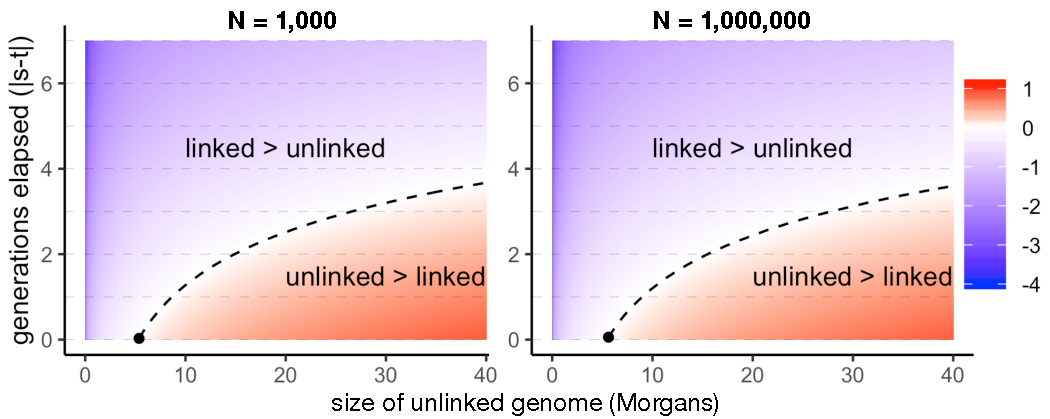
\includegraphics[]{./figures/unlinked_linked_contributions.pdf}

  \caption[The contribution of unlinked sites on a neutral site's
  autocovariance]{Here, we show the relative contributions of the linked and
    unlinked portions of the genome to the temporal autocovariance experienced
    by a neutral allele, for different generations elapsed (on the x-axis) and
    different map lengths of the unlinked genome (y-axis) for two different
    population sizes ($N=10^3$ and $N=10^6$). The color gradient is determined
    by the $\log_{10}$ value of the ratio of unlinked to linked contributions,
    the terms inside the braces in equation \eqref{eq:rel-contributions}. The
    dashed line indicates where the log ratio is zero, e.g. the relative
    contributions are equal; this was determined numerically. These assume LD
  is determined by mutation-drift-recombination balance
\parencite{Tomoko_Ohta1971-hb}.}

  \label{fig:linked-unlinked}
\end{figure}



\subsection{Averaging covariance across multiple loci}

Thus far, our covariance assumes that a single neutral site is positioned in
the center of a region $R$ Morgans long, with selected sites uniformly
distributed along this region. In our simulations, however, we simulate a
region that contains many neutral sites which we average over in calculating
the temporal autocovariance. In this case, we average over the random distance
between a neutral site's position $n$ and a selected site's position $g$, which
is $c = |n - g|$, where $n, g \sim U(0, R)$. This random variable $c$ is
distributed according to the triangle distribution, $f(c) = 2(R-c) / R^2$; we
replace the uniform PDF in Equation \eqref{eq:exp-overselpos} with the triangle
density PDF and average over the distance between sites,

\begin{align}
  \frac{\E_n(\cov(\Delta p_t, \Delta p_s))}{\E_n(p_t(1-p_t)) } %&=  \frac{V_a(s)}{2L} \sum_{l=1}^L \int_{0}^R \E(\mathcal{R}^2_{t}(r(c))) (1-r(c))^{s-t} \frac{2(R-c)}{R^2} d c \label{eq:exp-overselpos} \\
  &= \frac{V_a(s)}{2} \int_0^R \E(\mathcal{R}_t^2(r(c))) \; (1-r(c))^{(s-t)} \frac{2(R-c)}{R^2} \,d c \\
  &= \frac{V_a(s)}{2} \mathcal{A}(R, t, s)
\end{align}
%
where $\E_n(\cdot)$ indicates we take the expectation also over neutral sites,
and we use $\mathcal{A}(R, t,s)$ to denote the average linkage disequilibrium
between selected and neutral sites that persists from generations $t$ to $s$
($t \le s$). Note that in calculating the standardized covariance above, we use
a ratio of expectations rather than the expectation of the ratio
\parencite{Bhatia2013-zy}.

\subsection{Empirically Calculating the Average LD Persisting Across Generations}
\label{ap:empirical-ld}

In the previous expressions for temporal autocovariance, we stepped through a
conceptual model for the average levels of linkage disequilibria between
neutral and selected sites that persists across $|s-t|$ generations
($\mathcal{A}(R, t,s)$), where the positions of selected and neutral sites are
randomly distributed along a chromosomal region. In systems with a known
recombination map and studies where linkage disequilibria can be calculated, we
have the recombination fraction $r_{i,j}$ and the pairwise linkage
disequilibria $\mathbf{R}^2_{i,j}$ between between two loci $i$ and $j$ (where
$\mathbf{R}^2$ is the $M \times M$ matrix of pairwise LD calculated at time
$t$). Since we do not \emph{a priori} know whether a site is selected or not,
we sum over all polymorphic $M$ loci, thus characterizing the average
linkage disequilibria in a region as

\begin{align}
  \label{eq:supp-emp-assoc}
  \overline{\mathcal{A}(t, s)} = \frac{2}{M(M-1)} \sum_{i=1}^{M} \sum_{j > i} \mathbf{R}_{i,j}^2  (1-r_{i,j})^{|t-s|}.
\end{align}
%
This sum is the empirical analog to the integral in Equation
\eqref{eq:multilocus-triangle}.

\subsection{The Strength of Unlinked and Non-gametic Associations}
\label{ap:strength-assoc}

Here, we characterize the contribution of completely genetically unlinked loci
segregating for fitness variation to the change in frequency of our neutral
allele. Across evolutionary replicates, there is no expected covariance between
the neutral allele an individual carries and their fitness ($\E(\Delta_{_H}
p_t)= \E(\cov(x_i, f_i)) = 0$); rather, for unlinked loci, chance associations
are created from the variance around this sampling process of neutral alleles
into individuals with varying fitness ($\var(\Delta_{_H} p_t)= \var(\cov(x_i,
f_i))$). As the neutral allele and fitness variation independently assort
themselves into individuals, the chance associations that form have a variance
given by $\var(\cov_i(x_i, f_i))$.  This has the form of the sampling variance
of a covariance, which for random variables $X$ and $Y$ is given by
\citeauthor{Kendall1994-gp} (\citeyear{Kendall1994-gp}, p. 472),

\begin{align}
  \var(\cov(X, Y)) &= \frac{(n-1)^2}{n^3} (\mu_{22} - \mu_{11}^2) + \frac{n-1}{n^3} (\mu_{20}\mu_{02} - \mu_{11}^2)  \\
                   &\text{where} \; \mu_{rs} = \E(X-\mu_X)^r(Y-\mu_Y)^s)
\end{align}
%
where $\mu_X$ and $\mu_Y$ are the means of $X$ and $Y$ respectively, and
the variance is taken over conceptual replicate populations and the covariance
is calculated over the individuals in a population.  Then, applying this to
our covariance $\Delta_{_H} p_1 = \cov_i(x_i, f_i)$,

\begin{align}
  \label{eq:strength-assoc}
  \var(\Delta_{_H} p_1) &= \nicefrac{1}{4}\var(\cov_i(x_i, f_i)) \nonumber \\
                     &= \frac{(N-1)^2}{4N^3} \left(\E[(x_i - p_0)^2 (f_i - 1)^2] - \E[(x_i - p_0) (f_i - 1)]^2 \right)+ \nonumber \\
                     &\;\;\;\;\;\; \frac{N-1}{4N^3} \left(\E[(x_i - p_0)^2] \E[(f_i - 1)^2] - \E[(x_i -p_0)(f_i-1)]^2\right) \nonumber \\
                     &= \frac{(N-1)}{4N^3} \var(x_i) \var(f_i) \nonumber \\
                     &\approx \frac{p_0(1-p_0) }{2N} \var(f_i).
\end{align}
%
Thus the chance covariances that form between the neutral alleles individuals
carry and their fitness have a variance proportional to
$\nicefrac{\var(f_i)}{2N}$. 

\paragraph{Non-gametic linkage disequilibrium's contribution to temporal autocovariance}
\label{ap:non-gametic}

\begin{figure}[!ht]
  \centering
  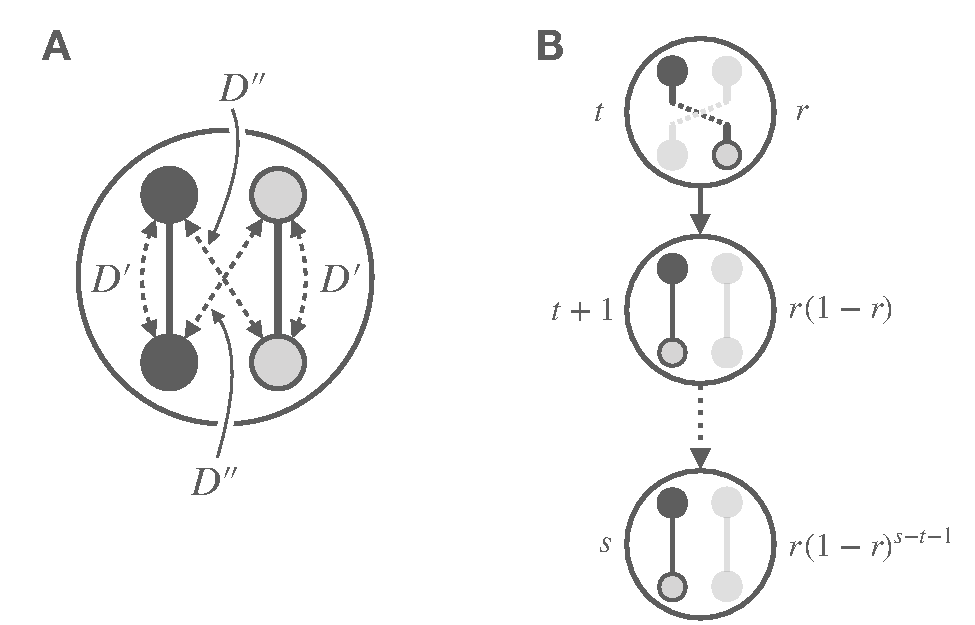
\includegraphics[scale=0.70]{./figures/keynote-cartoons-wide.pdf}

  \caption[Illustration of gametic and non-gametic LD]{A: An illustration of gametic ($D'$) and non-gametic ($D''$) linkage
    disequilibria between two loci in a diploid. B: An illustration of how
    non-gametic linkage disequilibria in generation $t$ is converted to gametic
    linkage disequilibria through recombination (which happens with probability
    $r$, the recombination fraction between the two loci), and is then
    maintained until generation $s$ with probability $(1-r)^{s-t-1}$. The gray
    loci on the gray gamete indicate the homologous, but not tracked focal
    association. Overall, the covariance created by the conversion of non-gametic
    LD to gametic LD is $\E(D_{s}' D_{t}'') = r(1-r)^{s-t-1}\E\left((D_{t}'')^2\right)$.}

  \label{fig:ld-cartoon}
\end{figure}


Throughout the paper, we ignore the effects of non-gametic linkage
disequilibria, $D_{t,l}''$, the disequilibria that occurs between the two
gametes (maternal and paternal) at two loci (see Figure \ref{fig:ld-cartoon}
(A) for an illustration of gametic LD $D'$ and non-gametic LD $D''$). Following
Weir's equation for the sampling variance of non-gametic LD $D_{A/B}$ (p. 124,
\citeyear{Weir1996-mv}), the chance non-gametic disequilibrium that builds up
sampling $2N$ gametes into $N$ individuals is,

\begin{align}
  \E\left((D_{t,l}'')^2\right) = \var(D_{A/B})  = \frac{1}{2N} p_A (1-p_A) p_B (1-p_B).
  \label{eq:non-gametic}
\end{align}
%
Note the similar form to Equation \eqref{eq:strength-assoc} as both the
unlinked and non-gametic LD arise from the random sampling of alleles at
different loci into individuals.

There is no expected covariance between our gametic and non-gametic LD within a
generation $\E(D_{t,l}'', D_{t,l}')=0$, assuming random mating. However,
$\E(D_{t,l}'',D_{s,l}')>0$ for $s>t$, as a fraction of the non-gametic LD
may be converted into gametic LD in the next generation. Specifically,
following Santiago and Caballero (\citeyear{Santiago1995-hx}), we can write the
product of the non-gametic LD in generation $t$ with the gametic LD in
generation $s$ as

\begin{equation}
  \E(D_{t,l}'',D_{s,l}') = r(1-r)^{(s-t-1)} \E\left((D_{t,l}'')^2\right)
  \end{equation}
%
where a proportion $r$ the non-gametic LD in generation $t$ is converted into
gametic LD, and a proportion $(1-r)^{(s-t-1)}$ of this is carried forward
unbroken by recombination over the remaining $s-t-1$ generations (see Figure
\ref{fig:ld-cartoon}B for an illustration of this process).

In our analysis in the main text, we ignore these terms as $D_{t,l}''$ is
expected to be small due to its inverse dependence on $N$. However, these terms
are necessary for the analysis of looser linkage
\parencite{Santiago1995-hx,Santiago1998-bs}. 

\subsection{Connecting our model with the models of Robertson (1961) and Santiago and Caballero (1995, 1998)}
\label{ap:connecting-sc}

Here, we describe the models of \textcite{Santiago1995-hx,Santiago1998-bs},
relating their work on the long-run effective population size experienced by a
neutral allele where there is (1) unlinked heritable fitness variation (their
1995 paper), or (2) linkage, where fitness-determining sites are randomly
scattered along a chromosome (their 1998 paper). Overall, their models are
formulated in a quantitative genetics tradition, where the population genetic
dynamics at the selected loci are not explicitly modeled (although these links
are made more explicitly in their '98 paper). In contrast, in deriving our
expressions for temporal autocovariance and variances, we use a population
genetic approach, modeling the dynamics at selected sites (though we simplify
from the full multilocus treatment, e.g. we assume selected loci experience
independent sweeps and we ignore the LD between selected sites). We show that
we can reconcile the two approaches, and demonstrate that the temporal
autocovariance expressions we develop in our models are implicit in their
model. We also work through their expressions for $N_e$ with heritable
variance, because it represents a quite useful result but their original
presentation was spread across two papers (and a change in notation).

\paragraph{Santiago and Caballero's 1995 and 1998 models for $N_e$}

While our goal in the main text of our paper was to develop expressions for the
temporal variances and autocovariances in allele frequency change when there is
heritable fitness variation in the population, the goal of both the 1995 and
1998 Santiago and Caballero papers is to derive an expression for the long-run
$N_e$ when there is heritable variation for fitness in the population. In their
1995 paper, they find the effective population size for large $t$ (see p. 1018,
equation 16) to be

\begin{align}
  N_e &= \lim_{t \to \infty} \frac{p_0(1-p_0) - \var(p_{t-1})}{2(\var(p_t) - \var(p_{t-1}))}  \\
  N_e &= \frac{4N}{2 + V_n + Q^2 C^2}
\end{align}
%

where $C^2$ is the heritable variation for fitness ($V_A$ in our notation), and
$V_n$ is the non-heritable variation in offspring number (i.e. under a
Wright--Fisher model, $V_n \approx 2$). For a neutral locus completely unlinked
from fitness variation (the situation first considered by
\cite{Robertson1961-ho}), $Q = 1 + \nicefrac{G}{2} + (\nicefrac{G}{2})^2 +
(\nicefrac{G}{2})^3 + \ldots = \sum_{i=0}^\infty (\nicefrac{G}{2})^i =
\nicefrac{2}{(2 - G)}$ (\cite{Santiago1995-hx}, equation 17). Here, $G$
represents the decay rate of the additive genetic variance associated with a
particular haplotype. Note that we've simplified their expressions by assuming
no assortative mating, and that we try to follow their notation as closely as
possible (consequently, the $Q$ here is unrelated to the $Q_{t,s}$ of the main
text).  \textcite{Santiago1995-hx} assume that continual artificial selection
maintains a constant level $C^2$ of fitness variation in the population each
generation, yet the \emph{particular} fitness backgrounds the neutral allele is
stochastically associated only contributes a fraction $G$ in the next
generation, $G^2$ in the generation after, and so on, as selection reduces
genetic variation for fitness (note: in their 1998 paper, they use $Z$ instead
of $G$). Similarly, the associations between the neutral and fitness
backgrounds decay at a rate $\nicefrac{1}{2}$ due to independent assortment.
Note that \textcite{Robertson1961-ho} assumed that the fitness backgrounds that
become stochastically associated with the neutral allele do not experience any
decay in their fitness variation ($G=1$); in this case, $Q = 2$ as Robertson's
work found. With an arbitrary amount of linkage between the focal neutral and
fitness backgrounds, \textcite{Santiago1998-bs} show that only $Q$ is affected,
and derive an expression for $Q$ that only depends on $G$ and the size of the
genome in Morgans, $L$ (equation 6, \citeyear{Santiago1998-bs}). 

In our main text, we model the temporal autocovariance created by heritable
fitness variation, which also impacts the cumulative variance in allele
frequency change $\var(p_t - p_0)$. To illustrate how our model connects with
theirs, below is the cumulative variance in allele frequency change for three
generations in their 1995 notation, with the corresponding changes in allele
frequency below,

\begin{align}
  \var(p_3 - p_0) = \E & \left( \bigg( \underbrace{S_1 + D_1 + H_1}_{\Delta p_1} + \right. \nonumber \\
                             & \underbrace{ (1-r) G S_1 + S_2 + D_2 + H_2}_{\Delta p_2} + \nonumber \\
                             & \left.  \underbrace{ (1-r)^2 G^2 S_1 + (1-r) G S_2 + S_3 + D_3 + H_3}_{\Delta p_3} \bigg)^2 \right).
                             % &  \underbrace{ (1-r)^2 G^2 S_1 + (1-r) G S_2 + S_3 + D_3 + H_3}_{\Delta p_3} + \nonumber \\
                             % &  \left. \underbrace{ (1-r)^3 G^3 S_1 + (1-r)^2 G^2 S_2 + (1-r) G S_3 + S_4 + D_4 + H_4}_{\Delta p_4} \bigg)^2 \right) \nnn  \\
    \label{eq:sc-var4}
\end{align}
%
Grouping terms by the generation that the initial association was formed, we
see how \textcite{Santiago1995-hx} define the $Q_i$ terms in their notation,

\begin{align}
  \var(p_3 - p_0) = \E & \left( \bigg( \underbrace{S_1(1 + (1-r) G + (1-r)^2 G^2)}_{\text{creation and persistence of generation 1 associations} \;\; := \; S_1 Q_3} \right. +  D_1 + H_1+ \nonumber \\
                       & \underbrace{S_2(1 + (1-r) G)}_{\text{creation and persistence of generation 2 associations} \;\; := \; S_2 Q_2}+ D_2 + H_2 + \nonumber \\
                       &  \underbrace{S_3}_{\text{creation of generation 3 associations} \;\; := \; S_3 Q_1  }\left. + D_3 + H_3 \bigg)^2 \right). &
    \label{eq:scr-var2}
\end{align}
%
since the associations created in generation $i$ ($ 0 < i \le t$) persist with
probability $(1-r)^{t-i}$, with proportion $G^{t-i}$ of its original fitness
variation in generation $t$. In general, the cumulative impact of the
associations formed $i$ generations ago has coefficient $Q_i =
\sum_{j=0}^{i-1} (1-r)^j G^j$. Using these $Q_i$ terms simplifies this equation
to

\begin{align}
  \var(p_4 - p_0) &= \E \left( \bigg(  S_1 Q_4 + D_1 + H_1 + S_2 Q_3 + D_2 + H_2 + \right. \nonumber \\
                  & \;\;\;\;\;\;\;\;\;\;\; \left. S_3 Q_2 + D_3 + H_3 + S_4 Q_1 + D_4 + H_4 \bigg)^2 \right)
                  % &= \sum_{i=1}^4 \var(\Delta_{_N} p_i) + \var(\Delta_{_M} p_i) + \sum_{i,j}^4 \cov(\Delta_{_H} p_i, \Delta_{H} p_j)
\end{align}
%
or, in general,

\begin{align}
    \var(p_t - p_0) &= \sum_{i=1}^t \E(D_i^2) + \E(H_i^2) + Q_{t-i+1}^2 E(S_i^2).
\end{align}

Then, Santiago and Caballero (1995) note that assuming $V_n$, $C^2$, and
population size $N$ are constant across generations, the magnitude of all of
the effects $\E(D_i^2)$, $\E(H_i^2)$, and $\E(S_i^2)$ are constant across all
generations (for all $i$, so we omit the $i$ subscript for these terms), except
for a geometric decay due to drift at a rate $(1-\nicefrac{1}{2N_e})$ per
generation that effects all terms. Such that, when we include the decay in the
variance due to drift,

\begin{align}
  \var(p_t - p_0) &= \sum_{i=1}^t \left(\E(D^2) + \E(H^2) + Q_{i}^2 E(S^2) \right) \left( 1 - \frac{1}{2N_e} \right)^{t-i}
  \label{eq:var-sc}
\end{align}
%
(cf. p. 1018 of \cite{Santiago1995-hx}). In the long run, the variance in the
neutral allele's frequency change hits a balance. Many copies of the neutral
allele segregating in the population are on fitness backgrounds it has recently
become stochastically associated with, as segregation and recombination have
not broke these associations apart. A few copies of the neutral allele are on
fitness backgrounds they became associated with many generations ago, that have
by chance survived to remain associated. In all cases, the effect these
associations have on present-day allele frequency change is weakened by the
fact that natural selection has reduced the genetic variance of these fitness
backgrounds. Since the long-run variance in allele frequency under drift in a
Wright--Fisher population is

\begin{align}
  \var(p_t) = p_0(1-p_0) \left[1 - \left(1 - \frac{1}{2N}\right)^t \right].
  \label{eq:sc-Ne}
\end{align}

One can estimate the effective population size $N_e$ using the observed
difference in variances $\var(p_t)$ and $\var(p_{t-1})$. (Note that this is
a different long-run effective population size used by others, $N_e =
p_0(1-p_0) t / (2\var(p_t - p_0))$, \cite{Crow1970-wm}) Santiago and
Caballero use Equation \eqref{eq:sc-Ne}, taking the difference $\var(p_t) -
\var(p_{t-1})$ and rearranging to end up with the large $t$ estimator of $N_e$, 

\begin{align}
  N_e = \frac{p_0(1-p_0) - \var(p_{t-1})}{2(\var(p_t) - \var(p_{t-1}))}
\end{align}
%
(cf. p. 1018, \cite{Santiago1995-hx}). Rearranging,

\begin{align}
  2N_e(\var(p_t) - \var(p_{t-1})) &= p_0 (1-p_0) - \var(p_{t-1}) \nonumber \\
  2N_e \var(p_t) - 2N_e \var(p_{t-1}) + \var(p_{t-1}) &= p_0(1-p_0) \nonumber \\
  2N_e \bigg(\var(p_t) - \var(p_{t-1}) \left(1 - \frac{1}{2N_e} \right)\bigg) &= p_0(1-p_0).
  \label{eq:sc-N}
\end{align}

This very conveniently simplifies the sum in Equation \eqref{eq:var-sc}, as we
can show with the case of $t=3$,

\begin{align}
  \var(p_3) = &\left(\E(D^2)+\E(H^2)+Q_1^2 \E(S^2)\right) \left(1-\frac{1}{2 N_e}\right)^2 + \nonumber \\
              &\left(\E(D^2)+\E(H^2)+Q_2^2 \E(S^2)\right) \left(1-\frac{1}{2 N_e}\right) + \nonumber \\
              &\;\E(D^2)+\E(H^2)+Q_3^2 \E(S^2) \nonumber \\
  \var(p_2)\left(1-\frac{1}{2N_e}\right) = &\left(\E(D^2)+\E(H^2)+Q_1^2 \E(S^2)\right) \left(1-\frac{1}{2N_e}\right)^2 + \nonumber \\
                                         &\;(\E(D^2)+\E(H^2)+Q_2^2 \E(S^2)) \left(1-\frac{1}{2N_e}\right) \nonumber \\
  \var(p_3) - \var(p_2)\left(1-\frac{1}{2N_e}\right) = &\E(D^2) + \E(H^2) + Q_3^2 \E(S^2) \nnn
\end{align}

or, generally, 

\begin{align}
  \var(p_t) - \var(p_{t-1})\left(1-\frac{1}{2N_e}\right) &= \E(D^2) + \E(H^2) + Q_t^2 \E(S^2)
\end{align}
%
Inserting this into Equation \eqref{eq:sc-N}, the long-run effective population
size can be written as

\begin{align}
  N_e &= \frac{p_0(1-p_0)}{2\bigg(\var(p_t) - \var(p_{t-1}) \left(1 - \frac{1}{2N_e} \right)\bigg)} \nonumber \\
      &= \frac{p_0(1-p_0)}{2\left( \E(D^2) + \E(H^2) + Q_\infty^2 \E(S^2) \right)}
  \label{sc:ne-eqn}
\end{align}
%
where $Q_\infty = 1 + \nicefrac{1}{2} + \nicefrac{1}{4} + \ldots = 2$ in
Robertson's (\citeyear{Robertson1961-ho}) model, and $Q_\infty = 1/(1 - G
(1-r))$ in Santiago and Caballero's (1995) model. (Note: $r$ here represents
the recombination fraction between fitness variation and neutral sites, which
differs from \textcite{Santiago1995-hx} equation 17, where $r$ represents the
correlation between parental fitness).

Then, \textcite{Santiago1995-hx} show,

\begin{align}
  \E(S^2) &= \frac{p_0(1-p_0)}{2N} C^2 \\
  \E(D^2) &= \frac{p_0(1-p_0)}{2N} \frac{V_n}{4} \\
  \E(H^2) &= \frac{p_0(1-p_0)}{2N} \frac{1}{2}
\end{align}
%
(cf. \cite{Santiago1995-hx}, equation 11). Inserting these into Equation
\eqref{sc:ne-eqn}, we have

\begin{align}
  N_e &= \frac{4N}{2 + V_n + 4 Q_\infty^2 C^2}
\end{align}
%
which is a simplified version of Santiago and Caballero's equation 16, and
which further simplifies to $N_e = N$ when $V_n = 2$ and $C^2 = 0$, the
effective population size of a Wright--Fisher population of $N$ hermaphroditic
individuals.


\paragraph{The covariances caused by fitness associations}

With an understanding now of the basics of Santiago and Caballero's (1995,
1998) models, how they connect to our notation, and how they reach their
expression for the long-run effective population size, we turn now to finding
the temporal autocovariances implicit in their model. We start by looking at
the variance in allele frequency between generations $0$ and $4$ (Equation
\eqref{eq:sc-var4}), including an additional generation so the pattern is
clearer later,

\begin{align}
  \var(p_4 - p_0) = \E & \left( \bigg( \underbrace{S_1 + D_1 + H_1}_{\Delta p_1} + \right. \nonumber \\
                             & \underbrace{ (1-r) G S_1 + S_2 + D_2 + H_2}_{\Delta p_2} + \nonumber \\
                             &  \underbrace{ (1-r)^2 G^2 S_1 + (1-r) G S_2 + S_3 + D_3 + H_3}_{\Delta p_3} + \nonumber \\
                             &  \left. \underbrace{ (1-r)^3 G^3 S_1 + (1-r)^2 G^2 S_2 + (1-r) G S_3 + S_4 + D_4 + H_4}_{\Delta p_4} \bigg)^2 \right). \nnn 
\end{align}

The cross-terms like $\E(D_1 D_2)$, $\E(H_1 D_1)$ and $\E(S_1 S_2)$ are all expected
products of independent random variables, where the expectation of each random
variable is zero, and consequently are all zero. The only non-zero cross terms
are products of $\E(S_i^2)$. When we look at the covariances with the allele
frequency change in the initial generation and a later generation $s$,
$\cov(\Delta_{_H} p_1, \Delta_{_H} p_s)$,

\begin{align}
  \cov(\Delta_{_H} p_1, \Delta_{_H} p_1) &= \var(\Delta_{_H} p_1) = \E(S_1^2) \\
  \cov(\Delta_{_H} p_1, \Delta_{_H} p_2) &= \frac{\E(S_1^2) G}{2} (1-r) \\
  \cov(\Delta_{_H} p_1, \Delta_{_H} p_3) &= \frac{\E(S_1^2) G^2 }{2}(1-r)^2\\
  \cov(\Delta_{_H} p_1, \Delta_{_H} p_4) &= \frac{\E(S_1^2) G^3 }{2} (1-r)^3
\end{align}
%
where the $\nicefrac{1}{2}$ coefficient comes from the fact that in Santiago
and Caballero's work, the $\E(S_1^2)$ products represent \emph{both} the
$\cov(\Delta_{_H} p_t, \Delta_{_H} p_s)$ and $\cov(\Delta_{_H} p_s, \Delta_{_H}
p_t)$ terms, so a single temporal autocovariance in our notation is half 
their joint covariance term.

However, if our reference generation is different, say 2, the associations from
earlier generations that have persisted to that generation can also lead to
covariances to later generations. Looking at the covariances 

\begin{align}
  \cov(\Delta_{_H} p_2, \Delta_{_H} p_2) &= \frac{\E(S_2^2) + \E(S_1^2) (1-r) G}{2} \\
  \cov(\Delta_{_H} p_2, \Delta_{_H} p_3) &= \frac{\E(S_2^2) G  + \E(S_1^2) (1-r) G^2}{2} (1-r) \\
  \cov(\Delta_{_H} p_2, \Delta_{_H} p_4) &= \frac{\E(S_2^2) (1-r) G^2 + \E(S_1^2) (1-r)^2 G^3}{2} (1-r)2.
\end{align}

Likewise, the covariances $\cov(\Delta_{_H} p_3, \Delta_{_H} p_s)$ include the
associations that persist from earlier generations. In general, 

\begin{align}
  \cov(\Delta_{_H} p_t, \Delta_{_H} p_s) = \frac{1}{2}\sum_{i=1}^{t} \E(S_i^2) \left(G (1-r)\right)^{t + s - 2i}, \; \; \text{for} \; \; t \le s.
  \label{eq:sc-cov}
\end{align}

This expression is more complex than our expression for temporal autocovariance
because its modeling the LD in generation $t$ as it builds up from generations
1 to $t$. In contrast, our expressions for covariance incorporate all of this
build up of LD as the initial LD term $\E(\mathcal{R}_t)$ (for a single locus case). This
expression for autocovariance implied by Santiago and Caballero's (1995) work
matches our expression for autocovariance (for a single locus) when the
arbitrary first generation is $t$ rather than 1

\begin{align}
  \cov(\Delta_{_H} p_t, \Delta_{_H} p_s) &= \frac{\E(S_t^2)G^{s-t}}{2}  (1-r)^{s - t}, \; \; \text{for} \; \; t \le s.
\end{align}

Using the expression for $\E(S_t^2)$ (equivalent to $\var(\Delta_{_H} p_t)$ in
our notation) derived in Appendix Section \ref{ap:strength-assoc}, 

\begin{align}
  \frac{\cov(\Delta_{_H} p_t, \Delta_{_H} p_s)}{p_t(1-p_t)} &= \frac{C^2 G^{s-t}}{4N}  (1-r)^{s - t}, \; \; \text{for} \; \; t \le s.
\end{align}

This is analogous to Equation \eqref{eq:multilocus-cov-sum} for a single
locus, where $C^2 G^{s-t}$ is the additive variation in generation $s$
(equivalent to our $V_a(s)$), and the factor $\nicefrac{1}{2N}$ represents the
chance build up of LD between the neutral site and an unlinked fitness background.
In our expression, we condition on existing linkage disequilibrium $\E(\mathcal{R}_t^2)$
between the neutral site and its fitness background, whereas they assume a
buildup of linkage disequilibria to a drift-recombination equilibrium. We can
see this by returning to the $\Delta_{_H} p_4$ term of Equation
\eqref{eq:sc-var4},

\begin{align}
  \var(\Delta_{_H} p_4) &= \E\left( (1-r)^3 G^3 S_1 + (1-r)^2 G^2 S_2 + (1-r) G S_3 + S_4 + D_4 + H_4\right)^2  \\
                        &= (1-r)^5 G^5 \E(S_1^2) + (1-r)^4 G^4 \E(S_2^2) + (1-r)^2 G^2 \E(S_3)^2 + \E(S_4^2) 
\end{align}
%
where following Santiago and Caballero's (\citeyear{Santiago1995-hx}, p. 1018)
approach, we can replace each $\E(S_i)$ with $\E(S_i^2) =
\E(S^2)(1-\nicefrac{1}{2N})^{i-1}$ and let $G=1$ as we focus on the buildup of
LD. This gives us the general equation, 

\begin{align}
  \var(\Delta_{_H} p_t) = \E(S^2) \sum_{i=1}^t (1-r)^{2i} \left(1-\frac{1}{2N}\right)^{i-1}
\end{align}
%
and taking this geometric series to infinity converges (since $(1-r)^2
(1-\nicefrac{1}{2N}) < 1$) and replacing $\E(S^2)$ with the chance associations
that build up gametes sampled into individuals (Equation
\eqref{eq:strength-assoc}),

\begin{align}
  \E((\Delta_{_H} p_\infty)^2) &= \E(S^2) \sum_{i=1}^\infty (1-r)^{2i} \left(1-\frac{1}{2N}\right)^{i-1} \nonumber \\
                             &= \frac{\E(S^2)}{1-\nicefrac{1}{2N}} \sum_{i=1}^\infty \left((1-r)^2 \left(1-\frac{1}{2N}\right)\right)^{i} \nonumber \\
                             &= \frac{C^2 p_0(1-p_0)}{1-\nicefrac{1}{2N}} \frac{1}{1-(1-r)^2 (1-\nicefrac{1}{2N})}.
\end{align}
% 
When we assume $r \to 0$ and $1/N \to 0$ and $Nr$ is a constant, this gives us

\begin{align}
  \E(\mathcal{R}^2) = \frac{\E((\Delta_{_H} p_\infty)^2)}{C^2 p_0(1-p_0)} &\approx \frac{1}{1 + 4Nr}
\end{align}
%
which is analogous to the $\E(\mathcal{R}^2)$ measure of linkage disequilibrium,
standardized to rescale the fitness variation. The right-hand side is identical
to \citeauthor{Sved1971-dv}'s identity by descent equilibrium $\E(\mathcal{R}^2)$ under
drift-recombination balance (\citeyear{Sved1971-dv}). Note that our expression
can be recovered from Equation \eqref{eq:sc-cov} when the reference generation
$t \to \infty$ such that the LD hits its equilibrium level,

\begin{align}
  \frac{\cov(\Delta_{_H} p_t, \Delta_{_H} p_s)}{p_0(1-p_0)} &= \frac{1}{2} \underbrace{C^2 G^{s-t}}_{V_A(s)} \underbrace{\frac{1}{1 + 4Nr}}_{\E(\mathcal{R}_t^2)} (1-r)^{s-t}
\end{align}
%
which is identical to our expression for temporal autocovariance when initial
LD is due to a neutral drift-recombination balance, and the change in $V_A$
during selection is modeled as a geometric decay at rate $G$.  Note that the
terms in underbraces indicate the corresponding terms in Equation
\eqref{eq:multilocus-cov-sum} for a single locus.

\subsection{Multilocus simulation details}
\label{sec:supp-ml-sim}


\paragraph{Targeting an initial level of Additive Genetic Variation}
\label{sec:supp-ml-sim-va}

We choose $\theta$ for the coalescent simulations to target a total number of
segregating sites $L + M$, where $L$ is the number of selected sites (a
parameter we vary in our multilocus simulations), and at least $M=200$ randomly
placed neutral sites over which we can calculate the temporal autocovariance.
Then, the total number of target sites $M+L$ is then inflated by a factor of
1.5 to ensure a sufficient number of sites given the random mutation process.
The $L$ selected sites are randomly chosen from the segregating sites, and all
remaining mutations are neutral. Thus, using \citeauthor{Watterson1975-kt}'s
expression for the expected number of segregating sites under the coalescent
(\citeyear{Watterson1975-kt}), we have $\theta = 1.5(M+L) / (\gamma +
\log(2N))$ where $\gamma \approx 0.577$ is Euler's Gamma. Each of the $L$
selected sites is given a random effect size of $\pm \alpha$ with equal
probability, where we choose by targeting a specific level additive genic
variation $V_a = 2 \alpha^2 \sum_l^L p_l(1-p_l) = \alpha^2 SSH_L$ where $SSH_L
= 2 \sum_l^L p_l(1-p_l)$ is the sum of site heterozygosity of the $L$ neutrally
evolving sites that will be selected once selection begins. Under neutrality,
$\E(SSH_L) = \theta_L = L/(\gamma + \log(2N))$. Then, we set $\alpha =
\sqrt{\nicefrac{V_a}{\theta_L}}$. We empirically validate that our target genic
variation is close to the empirically observed level.

\paragraph{Choosing the simulation parameter range}
\label{sec:supp-ml-sim-param}

We simulate over a grid of parameter ranges, varying the number of loci $L$,
the target additive genic variation $V_a$ in the region (by varying $\alpha$),
and the recombination map length of the region $R$ in Morgans. We have varied
these parameters over ranges that encompass a wide range likely to be
encountered in natural populations. To do this, we found that additive genetic
variation for lifetime reproductive success varied over orders of magnitude,
from 0 (e.g. in male red deer, \textcite{Kruuk2000-xt}) to ~1.1 in male
red-billed gull \parencite{Teplitsky2009-oj}. These values of additive genetic
variation are for the entire genome (we write these as $V_{A,GW}$, where $GW$
indicates genome-wide); our simulations model a region of varying map length.
We expect most recombination map lengths to be roughly over the scale of $5-50$
Morgans in length, and we chose to investigate how temporal autocovariance
behaves across a spectrum of recombination, from a completed linked region
($R=0$), to the scale over which a strong classic hardsweeps could affect
diversity (0.5 centiMorgans) to a region where the ends are approximately
unlinked (4.5 Morgans), overall giving us a parameter range of $R \in \{0,
0.005, 0.01, 0.05, 0.1, 0.5, 1.5, 4.5\}$.  Over this grid of our region
recombination map lengths, and the total organism recombination map lengths, we
get a rough estimate of the number of regions we would expect with this level
of recombination in the organism's total genome, imagining homogeneous
recombination rate, by taking $G/R$. Using this estimate of the number of
regions in the genome, we calculate the genetic variation per region over our
grid of parameters as $\nicefrac{V_{A,GW} R}{G}$, and target a level of
additive genic variation per region $V_a$ equal to this regional additive
genetic variation $V_A$. From preliminary simulations, we had found we can not
detect much temporal autocovariance below $V_a < 0.001$ with the initial level
of linkage disequilibrium from mutation-drift balance, so we ignore parameters
less than this value (other than $V_a=0$ as a control). Additionally, to reduce
the number of simulations, we exclude $V_a > 0.1$ as this only excludes a small
region of the parameter grid and preliminary simulations demonstrated the
behavior of temporal autocovariance with high $V_a$ is evident with the
included values. Overall, this gives us a spectrum of target additive genic
variation per region of $V_a \in \{0.001, 0.002, 0.005, 0.01, 0.02, 0.05, 0.08,
0.1\}$.  Note that to prevent our plots from being too dense, we include only a
representative subset of this parameter grid in our figures.


\subsection{Accounting for allele frequency sampling noise}
\label{sec:sampling}

In practice, one will calculate the temporal variance-covariance matrix on
allele frequency trajectories calculated from sampled chromosomes from the
population. We assume a binomial sampling process, where $n$ chromosomes are
sampled from the population such that $\widetilde{p} = \nicefrac{X}{n}$, and $X
\sim \textrm{Binom}(p, n)$. We can then write $\widetilde{p}_t = p_t +
\varepsilon_t$, and our covariances can be written as

\begin{align}
  \cov(\Delta \widetilde{p_t}, \Delta \widetilde{p_s}) &= \cov(\widetilde{p}_{t+1} - \widetilde{p}_{t}, \widetilde{p}_{s+1} - \widetilde{p}_{s}) \nonumber \\
  &= \cov(p_{t+1} + \varepsilon_{t+1} - p_{t} - \varepsilon_{t}, p_{s+1} + \varepsilon_{s+1} - p_{s} - \varepsilon_{s}).
\end{align}
%
Note this simplifies to

\begin{align}
  \cov(\Delta \widetilde{p_t}, \Delta \widetilde{p_s}) &= \cov(p_{t+1} - p_{t}, p_{s+1} - p_{s}) \; \; \mathrm{if} \;\; |t-s| > 1,
\end{align}
%
since in these cases, the sampling noise at a timepoint is not shared between
the estimated allele frequency changes. However, if $|t - s| = 1$ the sampling
noise from timepoint $t+1$ is shared, biasing the sample estimate of
covariance:

\begin{align}
\cov(\Delta \widetilde{p_t}, \Delta \widetilde{p}_{t+1}) 
  &= \cov(p_{t+1} + \varepsilon_{t+1} - p_{t} - \varepsilon_{t}, p_{t+2} + \varepsilon_{t+2} - p_{t+1} - \varepsilon_{t+1}) \nonumber \\
  &= \cov( \Delta p_{t} + \varepsilon_{t+1} - \varepsilon_{t}, \Delta p_{t+1} + \varepsilon_{t+2} - \varepsilon_{t+1}) \nonumber \\
  &= \cov(\Delta p_{t}, \Delta p_{t+1}) - \var(\varepsilon_{t+1}).
\end{align}
%
Similarly, the variance ($t = s$) is biased, as it is impacted by the binomial
sampling noise too,
%

\begin{align} 
  \var(\Delta \widetilde{p_t}) &= \cov( \Delta p_{t} + \varepsilon_{t+1} - 
      \varepsilon_{t}, \Delta p_{t} + \varepsilon_{t+1} - \varepsilon_{t}) \nonumber \\ 
                               &= \var( \Delta p_{t} ) + \var(\varepsilon_{t+1}) +
\var(\varepsilon_{t}) \end{align}
%
In practice, these covariances are calculated over loci in a region or across the
entire genome. We assume that the tracked allele has been randomly swapped
(e.g. the tracked allele frequency is not systematically the minor, major, or
reference allele), such that $\E(\Delta p_{t,l}) = 0$ for all $t$ and $l$. Then,
the unbiased covariance estimate as calculated over loci is

\begin{align}
  \frac{1}{L} \sum_{l=1}^L \left(\Delta p_{t,l} \Delta p_{t+1,l} \right)  &=
  \frac{1}{L} \sum_{l=1}^L \Delta \widetilde{p}_{t,l} \Delta \widetilde{p}_{t+1,l}
  + \frac{1}{L} \sum_{l=1}^L \varepsilon_{t+1,l}^2.
\end{align}
%
Then, we can use an unbiased plugin estimate of the frequency sampling variance
$\E(\varepsilon_{t+1,l}^2) = \V(\varepsilon_{t+1,l}) =
\nicefrac{p_{t+1,l}(1-p_{t+1,l})}{(n_{t,l}-1)}$ \parencite[p. 191]{Nei1987-bx}
to estimate these bias terms, and add or subtract them from the estimator
accordingly. Accounting for finite sampling, the unbiased sample
variance-covariance matrix now has elements:

\begin{align}
  \label{eq:corrected-var}
  Q_{t,t+1} &=
  \frac{1}{L} \sum_{l=1}^L \Delta \widetilde{p}_{t,l} \Delta \widetilde{p}_{t+1,l}
  + \frac{1}{L} \sum_{l=1}^L \frac{p_{t+1,l}(1-p_{t+1,l})}{n_{t+1,l} - 1},
\end{align}
and variance

\begin{align}
  \label{eq:corrected-cov}
  Q_{t,t} &=
  \frac{1}{L} \sum_{l=1}^L (\Delta \widetilde{p}_{t,l})^2
  - \frac{1}{L} \sum_{l=1}^L \frac{p_{t,l}(1-p_{t,l})}{n_{t,l} - 1}
  - \frac{1}{L} \sum_{l=1}^L \frac{p_{t+1,l}(1-p_{t+1,l})}{n_{t+1,l} - 1}.
\end{align}

In Section \ref{sec:ml-sim-res}, we used population frequencies in
introducing the method of moments estimators of $\widehat{V_A(1)}$ and
$\widehat{N}$. Here, we discuss the performance of these estimators with sample
allele frequencies. Our simulations are identical to those described in Section
\ref{sec:ml-sim}, except we have increased the target number of neutral sites
in each region so it is around $10,000$. We mimic sampling of $n=\{50, 100,
200, 500\}$ chromosomes from the population, and use the bias-corrected
sample variance-covariance matrix in the method-of-moments approach described
in Section \ref{sec:meth-moments} to estimate $\widehat{V_A(1)}$ and
$\widehat{N}$.

In Figure \ref{fig:mom-fits-both-finite}, we show the performance of our
estimators in the case where $n=100$ chromosomes have been sampled from the
population. Overall, there are two important differences compared with Figure
\ref{fig:mom-fits-both} of the main text. First, while the estimator
$\widehat{V_A(1)}$ performs well for high levels around $V_A \sim 0.1$, the
variance around the estimator increases significantly as $V_A$ grows weaker.
As the covariances are proportional to $\nicefrac{V_A}{R}$, sampling noise
grows larger than the theoretical temporal autocovariance as $V_A$ become weaker.
Then, one cannot discriminate against the chance covariances formed by the
sampling process from the temporal autocovariance created by linked selection
without either a large sample size or more timepoints. Second, the approach
underestimates $V_A(1)$ for very loose linkage ($R > \nicefrac{1}{2}$). This is
another consequence of the first problem; as sampling noise grows equal, or
larger than the magnitude of temporal autocovariance, the estimation procedure
performs poorly. As the linkage becomes more loose, the magnitude of temporal
autocovariance grows weak relative to the sampling noise, and this noise can be
partially absorbed by $\widehat{N}$. This effect can be somewhat ameliorated by
calculating the sample variance-covariance matrix over a shorter region of the
genome such that $R$ is smaller (as long as SNP density is sufficient), or by
increasing the sample size. Finally, the estimation of effective population
size shown in Figure \ref{fig:mom-fits-both-finite} are also affected by $V_A$,
as discussed in Section \ref{sec:meth-moments} (though the effect is obscured
by the sampling noise): high levels of $V_A$ in regions with low recombination
generally lead to underestimates of $\widehat{N}$.

To understand how sample size affects the method-of-moments estimators, Figure
\ref{fig:mom-relative} depicts median relative error of $\widehat{V_A(1)}$ and
$\widehat{N}$ for various sample sizes.


\begin{figure}
  \centering
  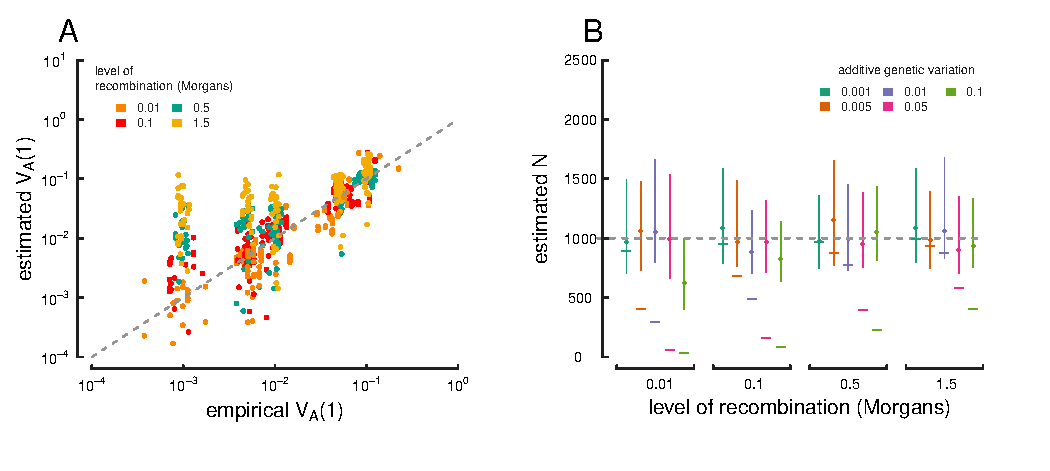
\includegraphics[width=\textwidth]{./figures/mom-fits-both-alt-finite.pdf} 

  \caption[Method of moment estimations for $V_A$ and $N$, conducted on samples
  of allele frequencies]{True parameter values and estimates using the
    method-of-moments approach on sample ($n=100$ chromosomes) multilocus
    simulation data; these figures are analogous to Figure
    \ref{fig:mom-fits-both} in the main text, except the estimators have been
    calculated on sample, rather than population frequency data. (A) The true
    $V_A(1)$ (x-axis) and $\widehat{V_A(1)}$ estimated from the sample
    variance/covariance matrix (y-axis) for each simulation replicate across
    different levels of recombination (indicated by each point's color). (B)
    Estimated drift-effective population size ($\widehat{N}$) across a range of
    simulations with different levels of additive genetic variance and
    recombination. Each point denotes the median, with lines denoting the
    interquartile range. A simple temporal estimate of the effective population
    size, estimated with accounting for the effects of selection, is averaged
  for each replicate and plotted as a dash. The true value ($N = 1,000$) is
shown with the dashed gray line.}

\label{fig:mom-fits-both-finite}
\end{figure}


\begin{figure}
  \centering
  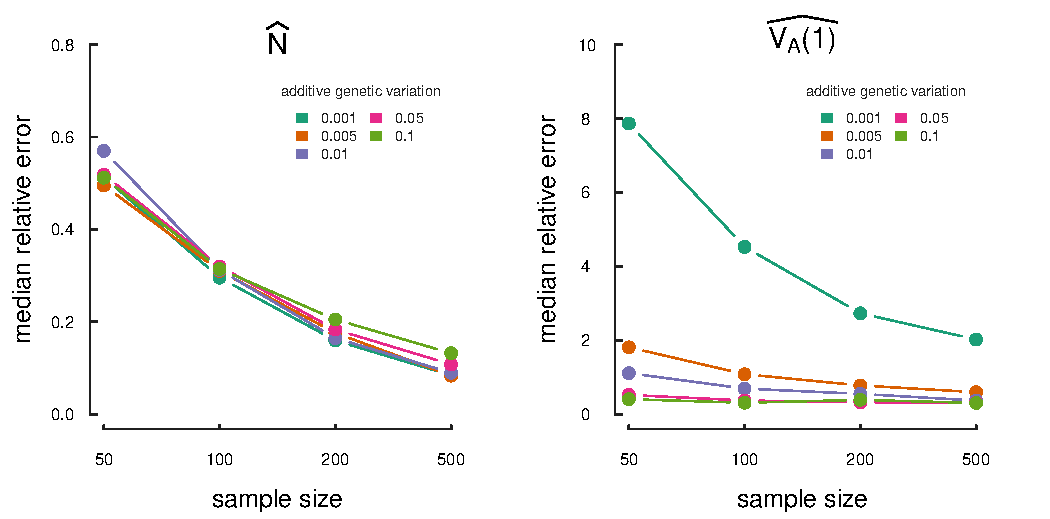
\includegraphics[width=\textwidth]{./figures/supp-relative-error.pdf} 

  \caption[Relative error of $N$ and $V_A$ estimates]{The median relative estimation error, over 30 replicate simulations,
  of the method of moments estimator for drift effective population size
($\widehat{N}$) and the initial additive genetic variance ($\widehat{V_A(1)}$).
} 

\label{fig:mom-relative}
\end{figure}




\newpage
\subsection{Appendix Figures}

\subsubsection{Validation of simulation routine}

\begin{figure}[!ht]
  \centering
  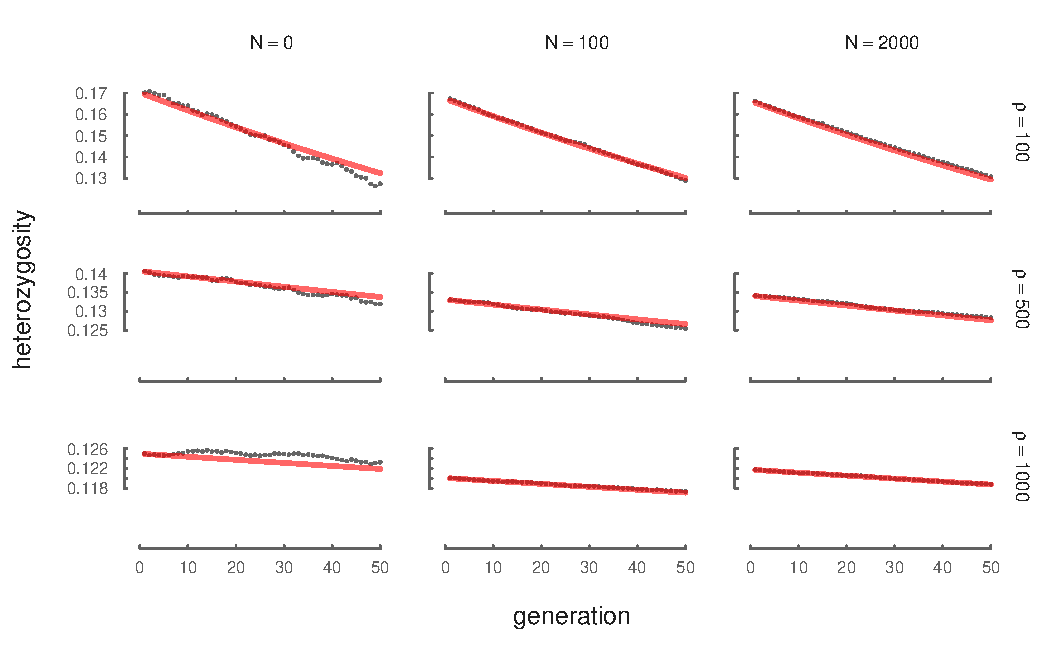
\includegraphics[width=\textwidth]{./figures/supp-het-neutral.pdf}

  \caption[Validation of simulation procedures: The neutral decay of heterozygosity]{The neutral decay of heterozygosity due to drift, averaged across 100
replicates and a variety of $N$ and $\rho$ levels. The red line is the
theoretical expectation $H_t = H_1 (1-1/(2N))^{t-1}$.}

\label{fig:het-neut}
\end{figure}


\begin{figure}[!ht]
  \centering
  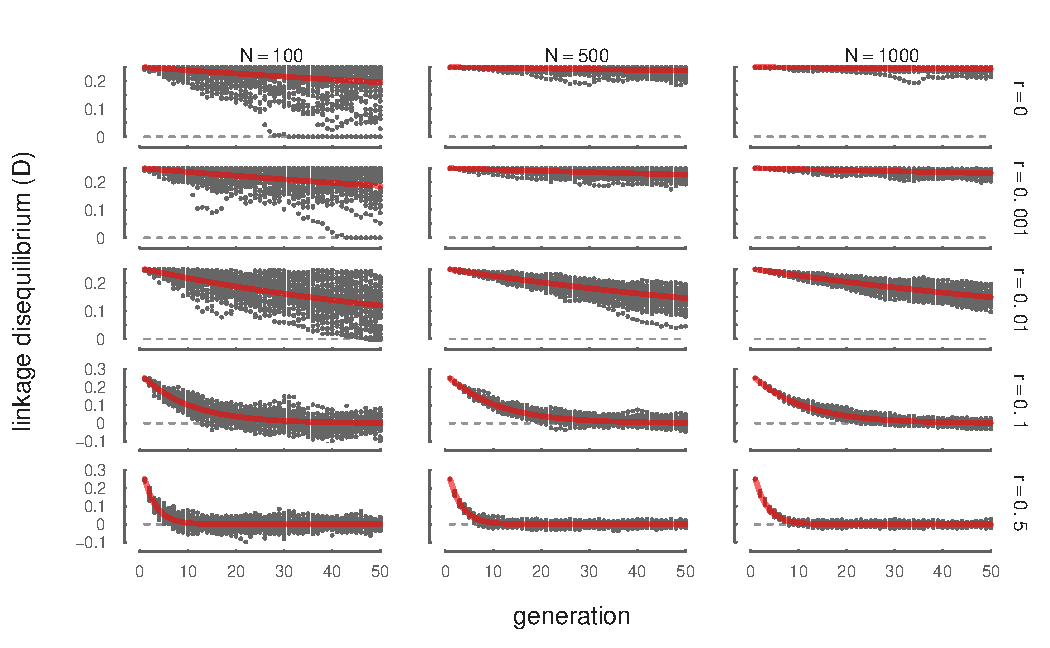
\includegraphics[width=\textwidth]{./figures/supp-ld-neutral.pdf}

  \caption[Validation of simulation procedures: The decay of LD]{The decay of LD between neutral sites due to recombination, across
    100 replicates and a variety of $V_A$ and $R$ levels. The initial
    population is created to have an artificial level of initial LD, with half
    the gametes carrying all derived alleles, and the other half carrying all
  ancestral alleles. The red line is the theoretical expectation $D_t = D_1 (1-1/(2N))^{t-1} (1-r)^{t-1}$.}

  \label{fig:ld-neut}
\end{figure}


\begin{figure}[!ht] \centering
  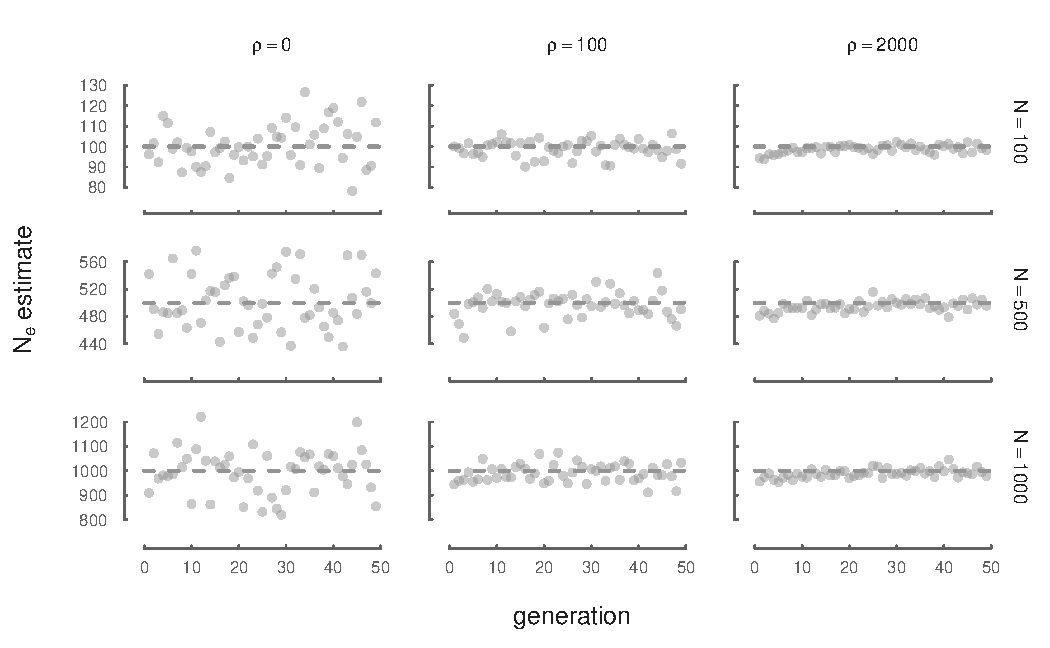
\includegraphics[width=\textwidth]{./figures/supp-Ne-est-neutral.pdf} 
  
  \caption[Validation of simulation procedures: Effective population sizes estimates]{$N_e$ estimated through time from neutral forward simulations is
  consistent with true $N$ across a variety of recombination $\rho$ and $N$
parameters. Here, we estimate $N_e$ with $\widehat{N_e} = \nicefrac{p(1-p)}{2
\var(\Delta p)}$ from neutral allele frequency changes.}

  \label{fig:ne-neut}
\end{figure}

\clearpage
\newpage

\subsubsection{Dynamics of Variances}

\begin{figure}[!ht]
  \centering
  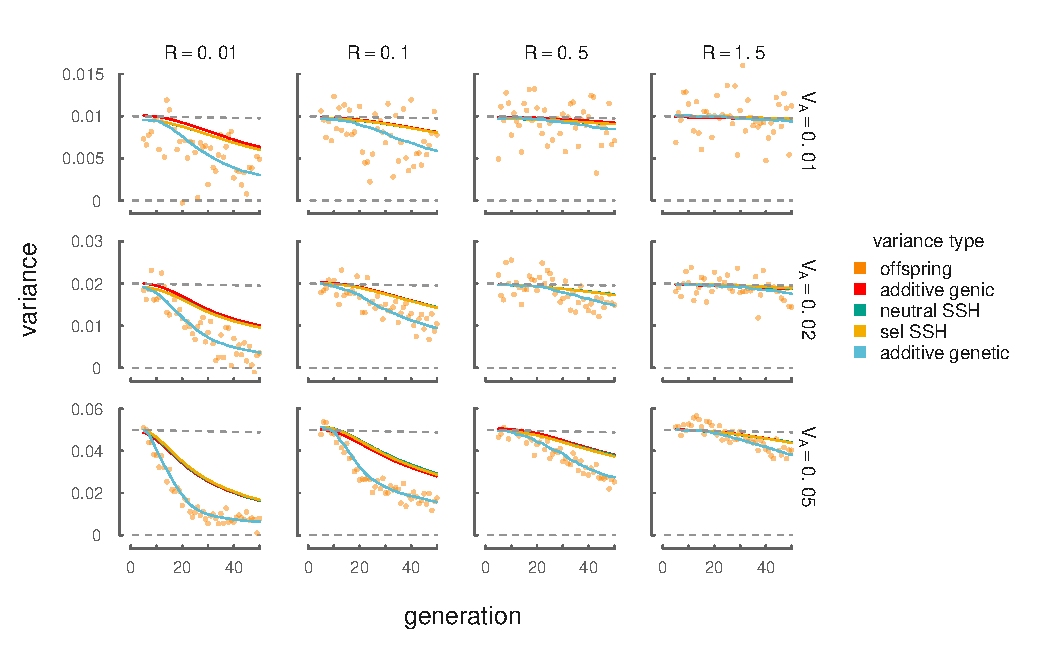
\includegraphics[width=\textwidth]{./figures/expfit-vark-types.pdf}
  \caption[Dynamics of differnt variances from our simulations during selection]{The dynamics of different variances in our simulations, across a
    variety of initial target $V_A$ and $R$ levels. Orange points represent the
    empirical heritable variance in offspring (e.g. with the noise of the
    Wright--Fisher reproduction process removed). These closely track the
    additive genetic variance for the trait undergoing directional selection,
    $V_A = \var(z)$. The red line shows the dynamics of additive genic
    variance, $V_a = 2 \sum_l \alpha_l^2 p_l(1-p_l)$, which is closely tracked
  by both the selected (yellow line) and neutral (green line) sum of site
heterozygosity proxies described in Section \ref{sec:dyn-var}.}

  \label{fig:multilocus-expfit-vark}
\end{figure}

\clearpage
\newpage

\subsubsection{Supplementary Temporal Autocovariance Figures}

\begin{figure}[!ht]
  \centering
  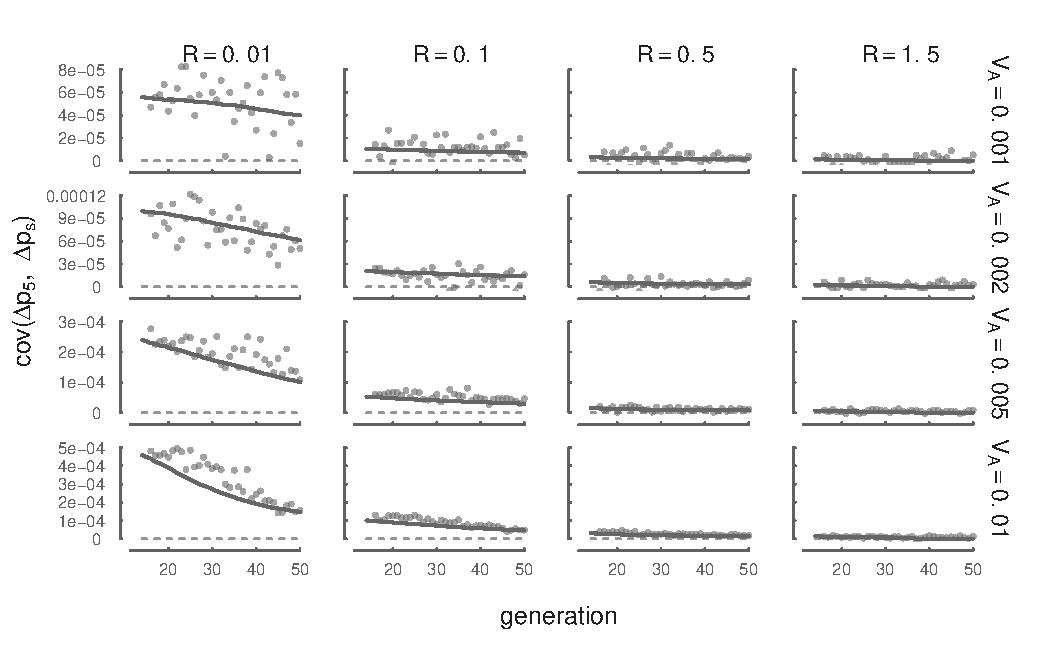
\includegraphics[width=\textwidth]{./figures/sim-pred13-covs-varyl.pdf}
  \caption[Temporal autocovariance simulation results and theoretical expectations from a different reference generation]{Each panel shows the temporal autocovariance $\cov(\Delta p_{13},
    \Delta p_s)$ on the y-axis, where $s$ varies along the x-axis. This is
    analogous to Figure \ref{fig:multilocus-expfit-sims} with a different
    reference generation ($t=13$), and compares the averaged simulation results
    (points) with the temporal autocovariance predicted by Equation
    \eqref{eq:multilocus-triangle} using the empirical additive genetic
    variance (curve). The covariances in these panels are weaker compared
    to those in Figure \ref{fig:multilocus-expfit-sims} because by generation
    13, additive genetic variance for fitness and the linkage disequilibria
    between neutral and selected sites has decayed.
}

\label{fig:multilocus-expfit-sims-gen13} 
\end{figure}


\begin{figure}[!ht]
  \centering
  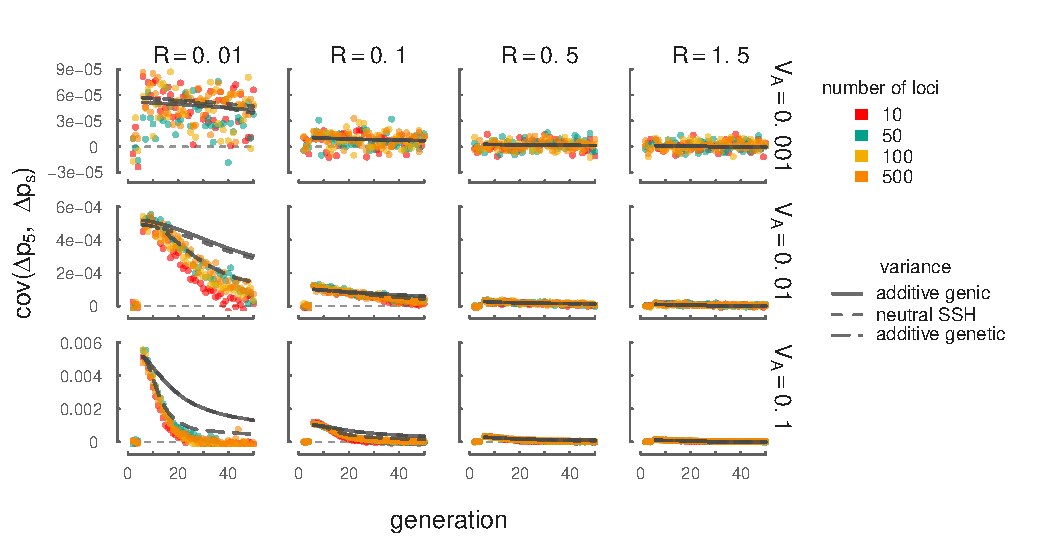
\includegraphics[width=\textwidth]{./figures/sim-pred-covs-varyl-va-oom.pdf}

  \caption[Simulation and theoretical expectations for a wider range of $V_A$ parameters]{A version of Figure \ref{fig:multilocus-expfit-sims} with a subset
    of $V_A$ parameters used in our simulations that vary over orders of
    magnitude. This demonstrates that our theory using the empirical additive
    genic variance (solid gray line), additive genetic variance (long dashed
    gray line), and the neutral SSH proxy (short dashed gray lines) performs as
    described in Section \ref{sec:ml-sim-res} even when $V_A$ varies over
    orders of magnitude in a region. Higher variance in the empirical
    covariances with weak selection ($V_A = 0.001$) are due to chance covariances
    due to drift. The light gray dashed line depicts $\cov(\Delta p_5, \Delta p_s) =
  0$.}
  

  \label{fig:multilocus-expfit-sims-va-oom}
\end{figure}

\begin{figure}[!ht]
  \centering
  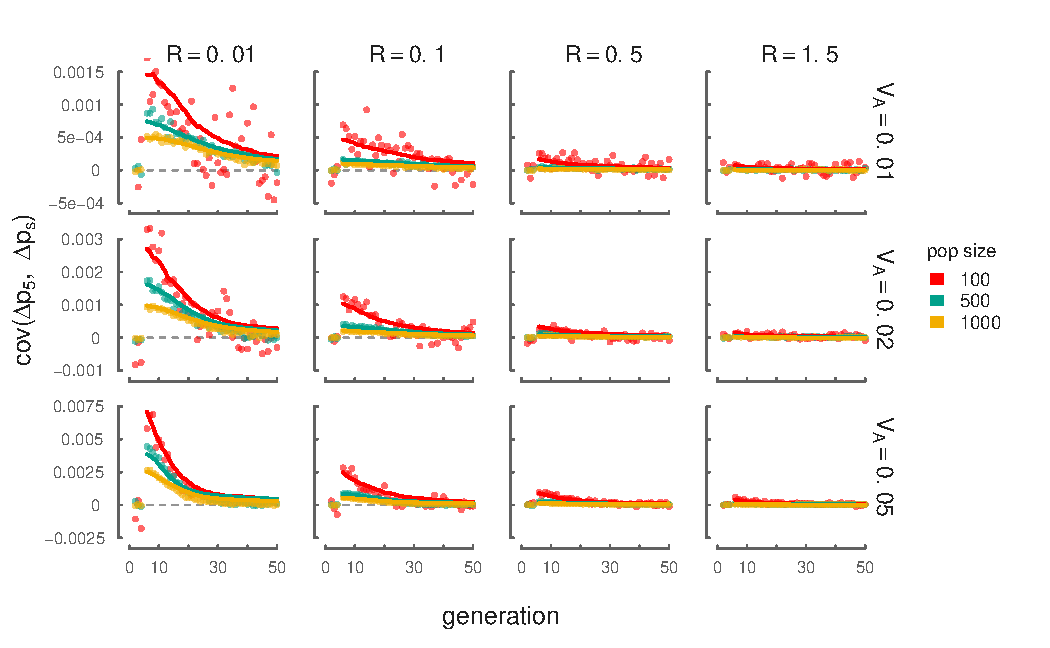
\includegraphics[width=\textwidth]{./figures/sim-pred-covs-varyn.pdf}

  \caption[Simulation and theoretical expectations for various $N$ parameters]{A version of Figure \ref{fig:multilocus-expfit-sims} demonstrating
    temporal autocovariance simulation results and theoretical predictions with
    varying $N$. This demonstrates that our theory using the empirical additive
    genetic variance (lines) fits simulations across a variety of $N$
    parameters.  The light gray dashed line depicts $\cov(\Delta p_5, \Delta p_s) =
  0$. Note that the initial LD varies due to differing equilibrium levels of
LD from our burnin across varying $N$.}

  \label{fig:multilocus-expfit-sims-varyn}
\end{figure}


\chapter{Estimating the contribution of selection to temporal allele frequency change}
\counterwithin{figure}{chapter}

\section{Introduction}

A long-standing problem in evolutionary genetics is quantifying the roles of
genetic drift and selection in shaping genome-wide allele frequency changes.
Selection can both directly and indirectly affect allele frequencies, with the
indirect effect coming from the action of selection on correlated loci
elsewhere in genome e.g. linked selection (\cite{Maynard_Smith1974-lc},
\cite{Charlesworth1993-gb,Nordborg1996-nq}; see \cite{Barton2000-zg} for a
review).  Previous work on this question has mostly focused on teasing apart
the impacts of drift and selection on genome-wide diversity using population
samples from a single contemporary timepoint, often by modeling the correlation
between regional recombination rate, gene density, and diversity created in the
presence of linked selection \parencite{Begun1992-ey,Elyashiv2016-vt}. This
approach has shown linked selection has a major role in shaping patterns of
genome-wide diversity across the genomes of some of organisms
\parencite{Begun2007-bg,Beissinger2016-cm,Sattath2011-dr,Williamson2014-oy,Andersen2012-bj,Cutter2010-gi},
and has allowed us to quantify the relative influence of positive selection
(hitchhiking) and negative selection (background selection;
\cite{Nordborg2005-dc,McVicker2009-ax,Hernandez2011-gs,Elyashiv2016-vt}.
However, we lack an understanding of how genome-wide linked selection acts over
time.

There are numerous examples of rapid phenotypic adaptation
\parencite{Grant2011-wk,Grant2006-hj,Reznick1997-mh,Franks2007-dr} and rapid
genomic evolution in asexual populations
\parencite{Good2017-om,Bennett1990-bc,Baym2016-kh}.  Yet the polygenic nature
of fitness makes detecting the impact selection on genome-wide variation over
short timescales in sexual populations remarkably difficult. This is because
the effect of selection on a polygenic trait (such as fitness) is distributed
across loci in proportion to their effect sizes. This can lead to subtle allele
frequency shifts on standing variation that are difficult to distinguish from
background levels of genetic drift and sampling variance.  However,
increasingly genomic experimental evolution studies with multiple timepoints,
and in some cases multiple replicate populations, are being used to detect
selected loci \parencite{Turner2011-sx,Turner2012-bm} and differentiate modes
of selection \parencite{Burke2010-tz,Barghi2019-qy,Therkildsen2019-zy}.  In
addition these temporal-genomic studies have begun in wild populations, some
with the goal of finding variants that exhibit frequency changes consistent
with fluctuating selection \parencite{Bergland2014-ij,Machado2018-cs}. In a
  previous paper, we proposed that one useful signal for understanding the
  genome-wide impact of polygenic linked selection detectable from temporal
genomic studies is the temporal autocovariance in allele frequency changes
\parencite{Buffalo2019-io}.  These covariances are directly estimable from
temporal genomic data and are created when the loci that underly heritable
fitness variation perturb the frequencies of linked neutral alleles; in
contrast, when genetic drift acts alone in a closed population, these
covariances are zero in expectation. Mathematically, temporal covariances are
useful because it is natural to decompose the total variance in allele
frequency change across a set of time intervals into the variances and
covariances in allele frequency change among time intervals.  Furthermore,
biologically, these covariances reflect the extent to which allele frequency
changes in one generation predict changes in another due to a shared fitness
background and shared selection pressures.

Here, we provide the first empirical analyses to quantify the impact of linked
selection acting over short timescales (tens of generations) across two evolve
and re-sequence studies \parencite{Barghi2019-qy,Kelly2019-dc}, and one
artificial selection experiment \parencite{Castro2019-uk}. We repeatedly find a
signal of temporal covariance, consistent with linked selection acting to
significantly perturb genome-wide allele frequency changes across the genome in
a manner that other approaches would not be able differentiate from genetic
drift. We estimate the lower bound on the proportion of total variation in
allele frequency change caused by linked selection, and the correlation between
allele frequency changes between replicate populations caused by response to
convergent selection pressures. Overall, we demonstrate that linked selection
has a powerful role in shaping genome-wide allele frequency changes over very
short timescales.

\clearpage
\section{Results}

\begin{singlespacing}
\begin{center}
  \captionof{table}{Summary of the studies reanalyzed.}
  \begin{tabular}{l c c c c c c}
    Study & Species & Selection & Replicates & Pop. Size & Gens. & Timepoints \\ 
  \hline
    \textcite{Kelly2019-dc}  & \emph{D. simulans} & lab & 3 & $\sim$1100 & 14 & 2 \\ \hline
    \textcite{Barghi2019-qy} & \emph{D. simulans} & lab & 10 & $\sim$1000 & 60 & 7 \\ \hline
    \textcite{Castro2019-uk} & \emph{M. musculus} & \begin{tabular}{c}tibiae length\\control\end{tabular} & \begin{tabular}{c}2\\1\end{tabular} &\begin{tabular}{c}32\\28\end{tabular}  & 20 & 2 \\
 \hline
\end{tabular}
\end{center}
\end{singlespacing}

We first analyzed \textcite{Barghi2019-qy}, an evolve-and-resequence study with
ten replicate populations exposed to a high temperature lab environment and
evolved for 60 generations, and sequenced every ten generations. Using the
seven timepoints and ten replicate populations, we estimated the genome-wide $6
\times 6$ temporal covariance matrix $\mathbf{Q}$ for each of the ten
replicates. Each row of these matrices represent the temporal covariance
$\cov(\Delta_{_{10}} p_s, \Delta_{_{10}} p_t)$, between the allele frequency
change (in ten-generation intervals, denoted $\Delta_{_{10}} p_t$) in some
initial reference generation $s$ (the row of the matrix), and some later
timepoint $t$ (the column of the matrix). We corrected these matrices for
biases created due to sampling noise, and normalize the entries for
heterozygosity (see Supplementary Material Sections
\ref{supp:ind-depth-var-corr} and \ref{supp:matrix-correction} for details on
the bias correction). The covariances are expected to be zero when only drift
is acting in a closed population, as only heritable variation for fitness can
create covariance between allele frequency changes \parencite{Buffalo2019-io}.
Averaging across the ten replicate temporal covariances matrices, we find
temporal covariances that are statistically significant (95\% block bootstraps
CIs do not contain zero), consistent with linked selection perturbing
genome-wide allele frequency changes over very short time periods. The
covariances between all adjacent time intervals are positive and then decay
towards zero as we look at more distant time intervals, as expected when
directional selection affects linked variants' frequency trajectories until
ultimately linkage disequilibrium and the additive genetic variance for fitness
associated with neutral alleles decays \parencite{Buffalo2019-io}. The temporal
covariances per replicate are noisier but this general pattern holds; see
Supplementary Figures \ref{suppfig:barghi-cov-panels}.
\textcite{Barghi2019-qy}'s design means that the covariances we see in adjacent
time intervals are on average ten generations apart, and given the temporal
decay in covariance we see, the covariances on shorter time-scales (e.g. if
adjacent generations had been sequenced) may well be higher yet (see
Supplementary Material Section \ref{supp:barghi-covs} for more details).

%We visualize these covariances in Figure \label{figure-1} (A), which
%depicts the temporal covariances through time, for each of the five
%off-diagonal rows temporal covariance matrix. Each row represents the temporal
%covariance $\cov(\Delta_{_{10}} p_s, \Delta_{_{10}} p_t)$, between some initial
%reference generation $s$ (the row of the matrix), and some later timepoint $t$
%(the column of the matrix). For each row, the covariances at first are
%positive, and then decay towards zero as expected when directional selection
%affects linked variants' frequency trajectories until ultimately linkage
%disequilibrium and additive genetic variance for decay
%\parencite{Buffalo2019-io}. Note that per replicate, the signal is a bit
%noisier; see Supplementary Figures XXX.

 
%Since the \textcite{Barghi2019-qy} study sequenced each
% replicate population every ten generations, we calculate the temporal
% covariance matrix over ten-generation allele frequency changes, which we write
% as $\cov(\Delta_{_{10}} p_s, \Delta_{_{10}} p_t)$. The diagonal elements of
% this temporal covariance matrix are the sum of all variances in allele
% frequency changes and pairwise covariances, e.g. element $\mathbf{Q}_{t,t} =
% \sum_{i=t}^{9} \var(\Delta p_i) + 2\sum_{i \ne j} \cov(\Delta p_i, \Delta
% p_j)$. Each off-diagonal element $\mathbf{Q}_{t,s}, \; t \ne s$ contains the
% sum of pairwise covariances, $\mathbf{Q}_{t,s} = \sum_{i=t}^{t+9}
% \sum_{j=s}^{s+9} \cov(\Delta p_i, \Delta p_j)$ (see Supplementary Material
% Section \ref{supp:barghi-covs} for more details). These off-diagonal
% covariances are expected to be zero when only drift is acting in the
% population, as only linked selection can create covariance between allele
% frequency changes \parencite{Buffalo2019-io}. Furthermore, since we cannot
% directly observe the temporal covariances between adjacent timepoints, but only
% the sums of temporal covariances, we expect the off-diagonal elements of
% $\mathbf{Q}$ to be weak. This is because the magnitude of a temporal covariance
% $\cov(\Delta p_i, \Delta p_j)$ is governed by the level of additive genetic
% variance and linkage disequilibrium that persists after $|i-j|$ generations of
% decay, which in \textcite{Barghi2019-qy}'s study design is on average 10
% generations.

\begin{figure}[!htb]
  \centering
  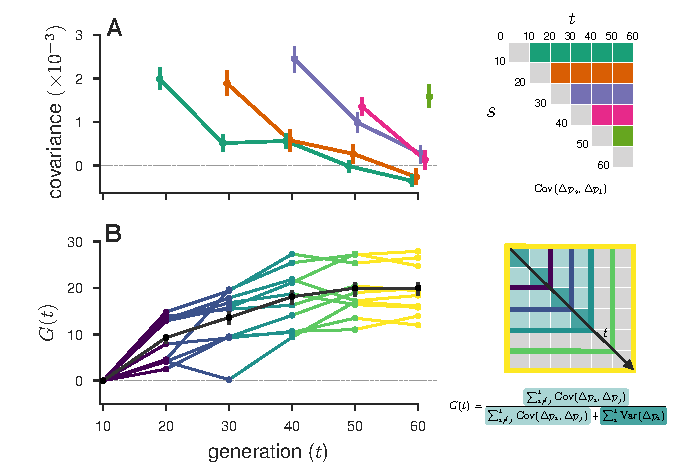
\includegraphics[width=\textwidth]{figures/figure-1.pdf}

  \caption[Temporal covariances and $G$ for \textcite{Barghi2019-qy} study]{A:
    Temporal covariance, averaged across all ten replicate populations, through
    time from the \textcite{Barghi2019-qy} study. Each line depicts the
    temporal covariance $\cov(\Delta p_s, \Delta p_t)$ from some reference
    generation $s$ to a later time $t$ which varies along the x-axis; each line
    corresponds to a row of the upper-triangle of the temporal covariance
    matrix with the same color (upper right). The ranges around each point are
    $95\%$ block-bootstrap confidence intervals. B: The proportion of the total
    variance in allele frequency change explained by linked selection, $G(t)$,
    as it varies through time $t$ along the x-axis.  The black line is the
    $G(t)$ averaged across replicates, with the $95\%$ block-bootstrap
    confidence interval. The other lines are the $G(t)$ for each individual
    replicate, with colors indicating what subset of the temporal-covariance
  matrix to the right is being included in the calculation of $G(t)$.}

  \label{fig:figure-1}
\end{figure}

While the presence of positive temporal covariances is consistent with linked
selection affecting allele frequencies over time, this measure not easily
interpretable. Additionally, we can quantify the impact of linked selection on
allele frequency change as the ratio of total covariance in allele frequency
change to the total variance in allele frequency change. {We denote the
change in allele frequency as $\Delta p_t = p_{t+1}-p_t$, where $p_t$ is the
allele frequency in generation $t$. Since the total variation in allele
frequency change can be partitioned into variance and covariance components,
$\var(p_t - p_0) = \sum_{i} \var(\Delta p_i) + \sum_{i \ne j} \cov(\Delta
p_i, \Delta p_j)$, and the covariances are zero when drift acts alone, this is
a lower bound on how much of the variance in allele frequency change is caused
by linked selection \parencite{Buffalo2019-io}. We call this measure $G(t)$, defined as

\begin{align}
  G(t) = \frac{\sum_{i\ne j}^t \cov(\Delta p_i, \Delta p_j)}{\var(p_t - p_0)}
\end{align}
%
which estimates the effect of linked selection between the initial
generation $0$ and some later generation $t$, which can be varied to see how
this quantity grows through time. As with the temporal covariances, the study
design of \textcite{Barghi2019-qy} leads our measure $G(t)$ to be even more
conservative, since the temporal covariances within each ten-generation block
between sequenced timepoints are not directly observable, and are not included
in the numerator of $G(t)$. Still, we find a remarkably strong signal.
Greater than $20\%$ of total variation in allele frequency change over 60
generations is the result of linked selection.

Additionally, we looked for a signal of temporal autocovariance in
\textcite{Bergland2014-ij}, a study that collected \emph{Drosophila
melanogaster} through Spring-Fall seasons across three years. With a pattern of
genome-wide fluctuating selection, we might expect a pattern of positive
covariances between similar seasonal changes, and negative covariances between
dissimilar seasonal changes. However, we find no such signal; we discuss this
in more depth in Supplementary Materials Section \ref{bergland-reanlysis}.

The replicate design of \textcite{Barghi2019-qy} allows us to quantify another
covariance: the covariance in allele frequency change between replicate
populations experiencing convergent selection pressures. These
between-replicate covariances are created in the same way as temporal
covariances: neutral alleles linked to a particular fitness background
experience are expected to have allele frequency changes in the same direction
if the selection pressures are similar. Intuitively, where temporal covariances
reflect that neutral alleles associated with heritable fitness backgrounds are
predictive of frequency changes between generations, replicate covariances
reflect that heritable fitness backgrounds common to each replicate predict
(under the same selection pressures) frequency changes between replicates. We
measure this through a statistic similar to a correlation, which we call the
convergent correlation: the ratio of average between-replicate covariance
across all pairs to the average standard deviation across all pairs of
replicates, 

\begin{align}
  \label{eq:conv-corr}
  \mathrm{cor}(\Delta p_s, \Delta p_t) = \frac{\E_{A\ne B} \left( \cov(\Delta p_{s,A}, \Delta p_{t,B}) \right)}{\E_{A\ne B} \left( \sqrt{\var(\Delta p_{s,A}) \var(\Delta p_{t,B})} \right)}
\end{align}
%
where $A$ and $B$ here are two replicate labels, and for the
\textcite{Barghi2019-qy} data, we use $\Delta_{_{10}} p_t$.

We've calculated the convergent correlation for all rows of the replicate
covariance matrices. Like temporal covariances, we visualize these through time
(Figure \ref{fig:figure-2} A), with each line representing the convergent
correlation from a particular reference generation $s$ as it varies with $t$
(shown on the x-axis). In other words, each of the colored lines corresponds to
the like-colored row of the convergence correlation matrix (upper left in
Figure \ref{fig:figure-2} A). We find these convergent covariances are
relatively weak, and decay very quickly from an initial value of about 0.1
(95\% block bootstrap confidence intervals $[0.094, 0.11]$) to around 0.01
(95\% CIs [0.0087, 0.015]) within 20 generations. This seems to confirm a
primary finding of the original \textcite{Barghi2019-qy} study: that
alternative loci contribute to adaptation in different replicates.

\begin{figure}[!htb]
  \centering
  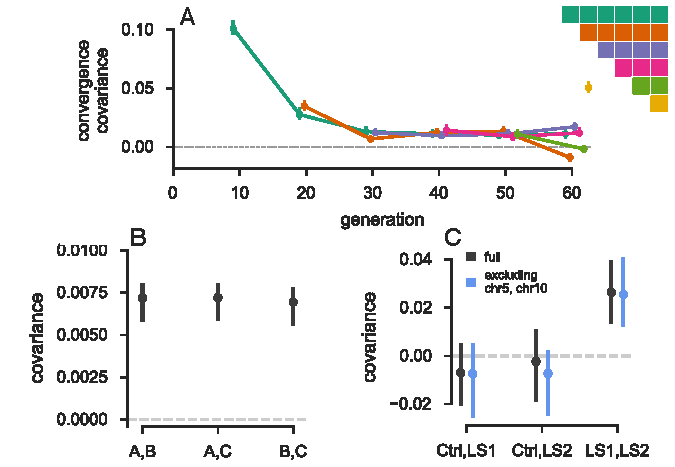
\includegraphics[width=\textwidth]{figures/figure-2.pdf}

  \caption[Convergence correlation \textcite{Barghi2019-qy} study]{{\bf A}: The
    convergence correlation, averaged across replicate pairs, through time.
    Each line represents the convergence correlation $\mathrm{cor}(\Delta
    p_{s}, \Delta p_{s})$ from a starting reference generation $s$ to a later
    time $t$, which varies along the x-axis; each line corresponds to a row of
    the temporal convergence correlation matrix depicted to the right.  {\bf
    B}: The convergence covariance between individual pairs of replicates in
    the \textcite{Kelly2019-dc} data. {\bf C}:  The convergence covariance
    between individual pairs of replicates in \parencite{Castro2019-uk} data,
    for the two selection lines  (LS1 and LS2) and the control (Ctrl); gray CIs
    are those using the complete dataset, blue CIs exclude chromosomes 5 and 10
    which harbor the two regions \textcite{Castro2019-uk} found to have signals
    of parallel selection between LS1 and LS2.}

  \label{fig:figure-2}
\end{figure}

% TODO \vince{GC: you had ??? here, not sure I see the issue.} 

A benefit of between-replicate covariances is that unlike temporal covariances,
these can be calculated with only two sequenced timepoints and a replicated
study design. This allowed us to assess the impact of linked selection in
driving convergent patterns of allele frequency change across replicate
populations in two other studies. First, we reanalyzed the selection experiment
of \textcite{Kelly2019-dc}, which evolved three replicate wild populations of
\emph{Drosophila simulans} for 14 generations adapting to a novel laboratory
environment. Since each replicate was exposed to the same selection pressure
and share linkage disequilibria common to the original natural founding
population, we expected each of the three replicate populations to have
positive between-replicate covariances. We find all three pairwise
between-replicate covariances are positive and statistically significant (95\%
CIs, [0.0063, 0.0086], [0.0064, 0.0086], [0.0061, 0.0083]). We estimate the
convergent correlation coefficient across these replicates as 0.36 ($95\%$
block-bootstrap confidence interval $[0.31, 0.40]$).

%\gc{TODO GIVE conversion \% var due to linked selection. }
Second, we reanalyzed the Longshanks selection experiment, which selected for
longer tibiae length relative to body size in mice, leading to a response to
selection of about 5 standard deviations over the course of twenty generations
\parencite{Castro2019-uk}. This study includes two independent selection lines,
Longshanks 1 and 2 (LS1 and LS2), and an unselected control line (Ctrl).
Consequently, this selection experiment offers a useful control to test our
between-replicate covariances: we expect to see positive between-replicate
covariance in the comparison between the two Longshanks selection lines, but
not between the two pairwise comparisons between the control line and the two
Longshanks lines. We find that this is the case (gray confidence intervals in
Figure \ref{fig:figure-2} C), with the two Longshanks comparisons to the
control line not being significantly different from zero, while the comparison
between the two Longshanks line is statistically significantly different from
zero (CIs [0.013, 0.037]).

A major finding in the Longshanks study were two major-effect loci that showed
parallel frequency shifts between the two selection lines: a region harboring
the gene Nkx3-2 known to be involved in limb development, and another region
harboring six other candidate genes. We were curious to what extent our
genome-wide covariances were being driven by these two outlier large-effect
loci, so we excluded them from the analysis. Since we do not know the extent to
which linkage disequilibrium around these large-effect loci affects neighboring
loci, we took the conservative precaution of excluding the entire chromosomes
these loci reside on (chromosomes 5 and 10), and re-calculating the temporal
covariances. We find excluding these large effect loci has little impact on the
confidence intervals (blue confidence intervals in Figure \ref{fig:figure-2}),
indicating that these across-replicate covariances are indeed driven by a
polygenic signal.

%We find that for covariances 2 timepoints apart ($k=2
%\times 10$ generations), the $20\%$ right tail is inflated by a of 1.3 (95\% CI
%[1.29, 1.32]), consistent with linked selection creating positive covariance in
%allele frequency change. Under constant directional selection, we expect these
%positive covariances between increasingly distant timepoints to decay to zero
%as additive genetic variance is exhausted by selection and linkage
%disequilibrium decays. Instead we find that for covariances 4 timepoints apart
%($k=4 \times 10$ generations), the left tail of negative covariances is
%inflated by a factor of 1.19 (95\% CI [1.17, 1.21]).

\begin{figure}
  \centering
  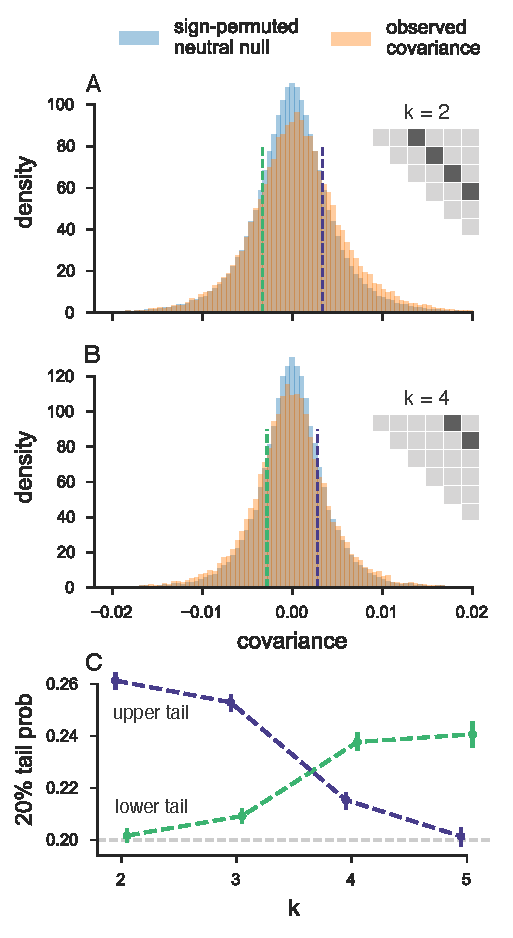
\includegraphics[]{figures/figure-3.pdf}

  \caption[Windowed covariance and empirical null distributions for the
  \textcite{Barghi2019-qy} study]{\footnotesize {\bf A}, {\bf B}: The
    distribution of temporal covariances calculated in 100kb genomic windows
    from the \textcite{Barghi2019-qy} study, plotted alongside an empirical
    neutral null distribution created by recalculating the windowed covariances
    on a 1,000 sign permutations of allele frequency changes within tiles. The
    histogram bin number is 88, chosen by cross validation (Supplementary
    Materials \ref{suppfig:barghi-cross-validation-binsize}). In subfigure {\bf
    A}, windowed covariances $\cov(\Delta p_t, \Delta p_{t+k})$ are separated
    by $k=2 \times 10$ generations and in subfigure {\bf A} the covariances are
    separated by $k=4 \times 10$ generations; each $k$ is an off-diagonal from
    the variance diagonal of the temporal covariance matrix (see cartoon of
    upper-triangle of covariance matrix in subfigures {\bf A} and {\bf B},
    where the first diagonal is the variance, and the dark gray indicates which
    off-diagonal of the covariance matrix is plotted in the histograms). {\bf
    C}: The lower and upper tail probabilities of the observed windowed
    covariances, at 20\% and 80\% quintiles of the empirical neutral null
    distribution, for varying time between allele frequency changes (i.e. which
    off-diagonal $k$). The confidence intervals are  $95\%$ block-bootstrap
  confidence intervals, and the light gray dashed line indicates the 20\% tail
probability expected under the neutral null.} 
\label{fig:figure-3}
\end{figure}

\clearpage


Finally, we observed that in the longest study  we analyzed
\parencite{Barghi2019-qy}, some genome-wide temporal covariances become
negative at future timepoints (see the first two rows in Figure
\ref{fig:figure-1} A). This shows that alleles that were on average going up
initially are later going down in frequency, i.e. that the average direction of
selection experienced by alleles has flipped. This must reflect either a change
in the environment or the genetic background, due to epistatic relationships
among alleles altered by frequency changes or recombination breaking up
selective alleles.  Such reversals of selective dynamics could be occurring at
other timepoints but the signal of a change in the direction of selection at
particular loci may be washed out when we calculate our genome-wide average
temporal covariances.  To address this limitation, we calculated the
distribution of the temporal covariances over 100kb genomic windows (Figure
\ref{fig:figure-3}, pooling across all replicates; see Supplementary Figure
\ref{suppfig:barghi-offset-replicate-panels} for individuals replicates). The
covariance of each tile will be noisy, due to sampling and genetic drift, and
the neutral distribution of the covariance is complicated due to linkage
disequilibria (which can occur over long physical distances in E\&R and
selection studies, \cite{Nuzhdin2013-gf,Baldwin-Brown2014-cl}). To address
this, we have developed a permutation-based procedure that constructs a null
distribution by randomly flipping the signs of the  allele frequency changes
per-genomic window. This destroys the systematic covariances created by linked
selection and creates a sampling distribution of the covariances spuriously
created by neutral genetic drift while preserving the complex dependencies
between adjacent loci created by linkage disequilibrium.  This empirical
neutral null distribution is conservative in the sense that the variances of
the covariances are wider than expected under drift alone as they include the
effect of selection on the allele frequency change within a time-interval, just
not between time-intervals. We see (Figure \ref{fig:figure-3} A and B) that
windowed temporal covariances between close timepoints are skewed positive (a
heavy right tail), while between more distant timepoints these windowed
temporal covariances tend to shift to become more negative (a heavy left tail).
We quantified the degree to which the left and right tails are inflated
compared to the null distribution as a function of time, and see excesses in
both tails in Figure \ref{fig:figure-3} C. This finding is also robust to
sign-permuting allele frequency changes on a chromosome-level, the longest
extent that gametic linkage disequilibria can extend (Supplementary Figure
\ref{suppfig:barghi-tailprobs-seqid}). We see a striking pattern that the
windowed covariances not only decay towards zero, but in fact become negative
through time, consistent with many regions in the genome having had a reversed
fitness effect at later timepoints.


\section{Discussion}

Since the seminal analysis of \textcite{Maynard_Smith1974-lc} demonstrating
that diversity is reduced at linked neutral variation as an advantageous
polymorphism sweeps to fixation, over four decades of theoretical and empirical
research has enriched our understanding of linked selection. This work has led
to the discovery of selected genes from genomic signals of hitchhiking
\parencite{Nair2003-tw,Voight2006-rn}, found genome-wide signals of linked
selection
\parencite{Aguade1989-jx,Begun1992-ey,Cutter2010-gi,Andersen2012-bj,Cutter2003-tl}
leading to the development of recurrent hitchhiking \parencite{Stephan1992-jc}
and background selection \parencite{Charlesworth1993-gb} models that attempt
explain this pattern. Since, much attention has focused on quantifying the
impact of background selection \parencite{McVicker2009-ax} and developing
theoretic machinery \parencite{Coop2012-cd} to differentiate the regional
reductions in diversity into those caused by full and partial sweeps, and those
caused by background selection \parencite{Elyashiv2016-vt}. However, as other
models of soft sweeps from standing variation emerged
\parencite{Hermisson2005-hs,Pennings2006-lj}, attention shifted towards
detecting other modes of linked selection \parencite{Pritchard2010-tk}, a more
difficult endeavor \parencite{Przeworski2005-bg} addressed using new coalescent
models \parencite{Berg2015-xj} and machine learning methods
\parencite{Schrider2017-yx}. An alternative approach to understanding the
genome-wide effects of selection on standing variation, e.g. selection on an
infinitesimal polygenic trait, stems from an early quantitative genetic model
of linked selection \parencite{Robertson1961-ho} and its later developments
(\cite{Santiago1995-hx,Santiago1998-bs}; see also \cite{Barton2000-zg} for a
comparison of these models with classic hitchhiking models). Implicit in these
models is that autocovariance between allele frequency change is created when
there is heritable fitness variation in the population, a signal that can be
readily detected from temporal genomic data \parencite{Buffalo2019-io}. Here,
we provide the first empirical evidence of linked selection acting on standing
variation over very short timescales.

We reanalyzed three published temporal genomic datasets and detected the
genome-wide signature of linked selection acting over tens of generations.
Furthermore, we find the dynamics of temporal autocovariance are consistent
with theory; the temporal covariance in allele frequencies decays as both
the fitness variation associated with particular haplotypes and the linkage
disequilibria between selected and neutral loci decay through time. In
reanalyzing one study \parencite{Barghi2019-qy}, we find that after sixty
generations, greater than 20\% of the variation in allele frequency change is
directly due to the action linked selection. Capitalizing on replicated
evolve-and-resequence study designs, we characterized the extent to which
convergent selection pressures lead to parallel changes in allele frequencies
across replicate populations, finding moderate correlations in allele frequency
changes.

While we must keep in mind that the studies analyzed here were all laboratory
populations and natural selection in the wild will likely differ, overall we
have found that linked selection has a remarkably strong effect for such short
study durations. Depending on how many loci affect fitness, such a strong
effect of linked selection may not be differentiable from genetic drift using
only single contemporary population samples. In this way, temporal data allows
us to sidestep the key problem of detecting selection from standing variation:
that the genomic footprint leaves too soft of a signature to differentiate from
a background of genetic drift. In fact we find that the temporal covariance
signal is detectable even in the most extremely difficult to detect soft sweep
case: polygenic selection on an infinitesimal trait. In our reanalysis of the
\textcite{Castro2019-uk} data, by showing the covariance signal remains even
after excluding the chromosomes containing two large-effect loci, we showed the
covariance signal we detect is indeed driven by polygenic fitness variation
(and confirm a point in the original study that tibiae length, aside from these
two large effect loci, is a highly polygenic trait).

It is worth building some intuition why temporal covariance allows us to detect
such faint signals of polygenic linked selection from temporal genomic data.
Each variant is subject to both variance in allele frequency due to drift and
two levels of sampling noise (as individuals are sampled from the population
and reads are sampled from amplified DNA), which at any locus swamps the
temporal covariance signal and creates spurious covariances. However, these
spurious covariances do not share a common sign across timepoints whereas the
covariances created by linked selection do; consequently, averaging across the
entire genome, the temporal signal exceeds sampling noise.

One limitation of these analyses is that none of the studies we reanalyzed
estimated linkage disequilibria data for the evolved populations. Our theory of
temporal autocovariance tells us that the temporal autocovariances a neutral
site experiences is determined by the product of the expected linkage
disequilibrium and additive fitness variation that persists through the
generations \parencite{Buffalo2019-io}. This leads to a clear prediction:
regions of higher linkage disequilibrium and lower recombination should have
greater temporal autocovariance than regions with lower LD and higher
recombination. Unfortunately, we lack a high-resolution recombination map for
\emph{D. simulans} and while there are LD data for \emph{D. simulans}
\parencite{Signor2018-wg} we did not find a relationship between temporal
covariance and LD. 

% \graham{TODO Is important point. We'll likely need plots for supp}

We believe this is driven by the idiosyncratic nature of LD in
evolve-and-resequence populations \parencite{Nuzhdin2013-gf,Kelly2019-dc}, and
that we might find such a relationship if LD data from the evolved population
were available. Unfortunately, sequencing multiple timepoints is expensive and
the low-coverage and/or pooled-sequencing approaches common in these studies
prohibit estimating linkage disequilibrium. Future studies complete with LD
data and recombination maps would allow one to disentangle the influence of
closely linked sites from more distant sites in causing temporal
autocovariance, and allow us to better understand whether sites in high
recombination regions are free from the effects of linked selection.
Furthermore, such additional data would allow for localizing the effects of
temporal covariance, which would allow us to estimate not just the genome-wide
fraction of variation in frequency change ($G(t)$), but also the fraction of
the genome impacted by linked selection, allowing us to synthesize the temporal
approach with single-timepoint studies like that of \textcite{Elyashiv2016-vt}.

%Why the variation in convergence correlations?

Thus far, the most comprehensive studies implicating linked selection in
affecting genome-wide diversity have been in \emph{Drosophila}
\parencite{Begun1992-ey,Elyashiv2016-vt,Sattath2011-dr} and
\emph{Caenorhabditis} \parencite{Cutter2003-tl,Cutter2003-tl,Andersen2012-bj},
whereas the evidence for linked selection in plant and yeast species is weak
\parencite{Cutter2013-ba}. Both \emph{Drosophila} and \emph{Caenorhabditis}
have short genetic maps (or in the case of selfing \emph{C.  elegans}, small
effective recombination rates), and large effect population sizes, two factors
predicted to increase the degree to which hitchhiking impacts genome-wide
diversity \parencite{Barton2000-zg}. However, our results here show that even
with small effective population sizes (300, 450, and 45 for the
\textcite{Kelly2019-dc}, and \textcite{Castro2019-uk} studies respectively)
and, in the case of mice, moderately-sized genetic maps (around 14 Morgans;
\cite{Cox2009-hf}), we still see a fairly strong effect of linked selection.
This suggests that while these factors may govern the dynamics of classic
hitchhiking events, they could perhaps play less of a role in polygenic linked
selection. However, with only three cases analyzed, further studies on
different taxa are needed.

Finally, in reanalyzing the \textcite{Barghi2019-qy} study, we find evidence
of complex linked selection dynamics. This is due either to a change in the
environment and its consequences for the fitness of regions in the genome,
recombination breaking up selected alleles, or epistatic interactions between
loci. It is important to note that the original study did not intentionally
alter the environment in any way; this signal is attained without intentionally
seeking it out. Discerning which of these is creating negative temporal
autocovariance is a sizable challenge, requiring sequencing each generation and
LD data.

Overall, we hope this will encourage more temporal genomic studies in both
laboratory and natural populations. Understanding the dynamics of linked
selection over short timescales will help to unite phenotypic studies of rapid
adaptation of polygenic adaptations with a detectable genomic signature, to
address long-standing questions concerning linked selection, evolutionary quantitative
genetics, and the overall impact selection has on genetic variation. 

\newpage

\section{Appendix}

\section{Estimator Bias Correction}
\subsection{Correcting variance bias with a single depth sampling process}
\label{supp:depth-var-corr}

Following \textcite{Waples1989-sj}, we have that that the variance in allele
frequency change at a locus in the initial generation, which is entirely due to
the binomial sampling process, is $\var(p_0) = \nicefrac{p_0(1-p_0)}{d_0}$
where $d_0$ is the number of binomial draws (e.g. read depth). At a later
timepoint, the variance in allele frequency is a result of both the binomial
sampling process at time $t$ and the evolutionary process. Using the law of
total variation we can partition the variation from each process,

\begin{align}
  \var(\widetilde{p_t}) &= \E(\var(\widetilde{p_t} | p_t)) + \var(\E(\widetilde{p_t}|p_t)) \\
                        &= \underbrace{\frac{p_t(1-p_t)}{d_t}}_\text{generation $t$ sampling noise} + \underbrace{\var(p_t)}_\text{variance due to evolutionary process}.
  %\frac{\var(\widetilde{p_t})}{p_0(1-p_0)} &= \frac{p_t(1-p_t)}{p_0(1-p_0) d_t} + 1 - \left( 1-\frac{1}{2N}\right)^t.
  %\frac{\var(\widetilde{p_t})}{p_0(1-p_0)} &= \frac{p_t(1-p_t)}{p_0(1-p_0) d_t} + \frac{t}{2N} + O\left((2 N)^{-2}\right).
\end{align}

Under a drift-only process, $\var(p_t) = p_0(1-p_0)\left[1- \left(1 -
\frac{1}{2N}\right)^t\right]$. However, with heritable variation in fitness, we
need to consider the covariance in allele frequency changes across generations
\parencite{Buffalo2019-io}. We can write

\begin{align}
  V(p_t) &= V\left(p_0 + (p_1 - p_0) + (p_2 - p_1) + \ldots + (p_t - p_{t-1}) \right) \\
         &= V\left(p_0 + \Delta p_0 + \Delta p_1 + \ldots + \Delta p_{t-1} \right) \\
         &= V(p_0) + \sum_{i=0}^{t-1} \cov(p_0, \Delta p_i) + \sum_{i=0}^{t-1} \var(\Delta p_i) + \sum_{0 \le i < j}^{t-1} \cov(\Delta p_i, \Delta p_j).
\end{align}
%

Each allele frequency change is equally like to be positive as it is to be
negative; thus by symmetry this second term is zero. Additionally $V(p_0) = 0$,
as we treat $p_0$ as a fixed initial frequency. We can write, 

\begin{align}
  V(p_t) &= \sum_{i=0}^{t-1} \var(\Delta p_i) + \sum_{0 \le i < j}^{t-1} \cov(\Delta p_i, \Delta p_j).
\end{align}

The second term, the cumulative impact of variance in allele frequency change
can be partitioned into heritable fitness and drift components
\parencite{Santiago1995-hx,Buffalo2019-io}

\begin{align}
  V(p_t) &= \sum_{i=0}^{t-1} \var(\Delta_{_D} p_i) + \sum_{i=0}^{t-1} \var(\Delta_{_H} p_i) + \sum_{0 \le i < j}^{t-1} \cov(\Delta p_i, \Delta p_j).
\end{align}

where $\Delta_{_H} p_t$ and $\Delta_{_D} p_t$ indicate the allele frequency
change due to heritable fitness variation and drift respectively. Then, sum of
drift variances in allele frequency change is

\begin{align}
  \sum_{i=0}^{t-1} \var(\Delta_{_D} p_i) = \sum_{i=0}^{t-1} \frac{p_i(1-p_i)}{2N}
\end{align}
%
replacing the heterozygosity in generation $i$ with its expectation, we have

\begin{align}
  \sum_{i=0}^{t-1} \var(\Delta_{_D} p_i) &= p_0(1-p_0) \sum_{i=0}^{t-1} \frac{1}{2N} \left(1-\frac{1}{2N}\right)^i \\
                                         &= p_0(1-p_0) \left[1 - \left(1-\frac{1}{2N}\right)^t \right]
\end{align}
%
which is the usual variance in allele frequency change due to drift.  Then, the
total allele frequency change from generations $0$ to $t$ is
$\var(\widetilde{p}_t - \widetilde{p}_0) = \var(\widetilde{p}_t) +
\var(\widetilde{p}_0) - 2 \cov(\widetilde{p}_t, \widetilde{p}_0)$, where the
covariance depends on the nature of the sampling plan (see \cite{Nei1981-oy,
Waples1989-sj}). In the case where there is heritable variation for fitness,
and using the fact that $\cov(\widetilde{p}_t, \widetilde{p}_0) =
\nicefrac{p_0(1-p_0)}{2N}$ for Plan I sampling procedures
\parencite{Waples1989-sj}, we write,

\begin{align}
  \var(\widetilde{p}_t - \widetilde{p}_0) &= \var(\widetilde{p}_t) + \var(\widetilde{p}_0) - 2 C \cov(\widetilde{p}_t, \widetilde{p}_0) \\
                                          &= \frac{p_t(1-p_t)}{d_t}  + \frac{p_0(1-p_0)}{d_0} + p_0(1-p_0) \left[1 - \left(1-\frac{1}{2N}\right)^t \right] + \\ & \;\;\;\;\;\;
                                               \sum_{i=0}^{t-1} \var(\Delta_{_H} p_i)  + \sum_{0 \le i < j}^{t-1} \cov(\Delta p_i, \Delta p_j) - \frac{C p_0(1-p_0)}{2N} \\
  \frac{\var(\widetilde{p}_t - \widetilde{p}_0)}{p_0(1-p_0)} &= 1 + \frac{p_t(1-p_t)}{p_0(1-p_0)d_t}  + \frac{1}{d_0} - \left(1-\frac{1}{2N}\right)^t + \\ & \;\;\;\;\;\;
  \sum_{i=0}^{t-1} \frac{\var(\Delta_{_H} p_i)}{p_0(1-p_0)}  + \sum_{0 \le i < j}^{t-1} \frac{\cov(\Delta p_i, \Delta p_j)}{p_0(1-p_0)} - \frac{C}{N}
\end{align}
%
where $C = 1$ if Plan I is used, and $C=0$ if Plan II is used (see
\cite{Waples1989-sj}, p. 380 and Figure 1 for a description of these sampling
procedures; throughout the paper we use sampling Plan II). We move terms
creating a bias-corrected estimator for the population variance in allele
frequency change, and replace all population heterozygosity terms with the
unbiased sample estimators, e.g. $\frac{d_t}{d_t-1} \widetilde{p}_t (1-
\widetilde{p}_t)$,

\begin{align}
  \label{supp:eqn-depth-only-correction}
  \frac{d_0-1}{d_0} \frac{\var(\widetilde{p}_1 - \widetilde{p}_0)}{\widetilde{p}_0(1-\widetilde{p}_0)} - \frac{(d_0-1)}{d_0 (d_1 - 1)} \frac{\widetilde{p}_1(1-\widetilde{p}_1)}{\widetilde{p}_0(1-\widetilde{p}_0)} - \frac{1}{d_0} + \frac{C}{N}  &= \frac{\var(\Delta_{_H} p_0)}{p_0(1-p_0)} + \frac{1}{2N} 
\end{align}

\subsection{Correcting variance bias with individual and depth sampling processes}
\label{supp:ind-depth-var-corr}

Here, we extend the sampling bias correction described above to handle two
binomial sampling processes: one as individuals are binomially sampled from the
population, and another as reads are binomially sampled during sequencing.
(see also \cite{Jonas2016-ia}). Let $X_t \sim \text{Binom}(n_t, p_t)$ where
$X_t$ is the count of alleles and $n_t$ is the number of diploids sampled at
time $t$. Then, these individuals are sequenced at a depth of $d_t$, and $Y_t
\sim \text{Binom}(d_t, \nicefrac{X_t}{n_t})$ reads have the tracked allele. We
let $\widetilde{p_t} = \nicefrac{Y_t}{d_t}$ be the observed sample allele
frequency. Then, the sampling noise is 

\begin{align}
  \var(\widetilde{p_t}|p_t) &= \E(\var(\widetilde{p_t} | X_t)) + \var(\E(\widetilde{p_t} | X_t)) \\
                            &= p_t(1-p_t) \left(\frac{1}{n_t} + \frac{1}{d_t} - \frac{1}{n_t d_t} \right)
\end{align}


\begin{align}
  \var(\widetilde{p}_t - \widetilde{p}_0) &= 
  p_t(1-p_t) \left(\frac{1}{n_t} + \frac{1}{d_t} - \frac{1}{n_t d_t} \right)  
  + p_0(1-p_0) \left( \frac{1}{n_0} + \frac{1}{d_0} - \frac{1}{n_0 d_0}\right)  \\ & \;\;\;\;\;\;
  - \frac{C p_0(1-p_0)}{N} + p_0(1-p_0) \left[1 - \left(1-\frac{1}{2N}\right)^t \right]+ \sum_{i=0}^{t-1} \var(\Delta_{_H} p_i)  \\ & \;\;\;\;\;\; + \sum_{0 \le i < j}^{t-1} \cov(\Delta p_i, \Delta p_j) 
\end{align}
%
Through the law of total expectation (see \cite{Kolaczkowski2011-ee}
Supplementary File 1 for a sample proof), one can find that an unbiased
estimator of the half the heterozygosity is 

\begin{align}
  \frac{n_t d_t}{(n_t-1) (d_t-1)} \widetilde{p_t}(1-\widetilde{p_t}).
\end{align}
%
Replacing this unbiased estimator for half of the heterozygosity into our
expression above, the total sample variance is

\begin{align}
  \var(\widetilde{p}_t - \widetilde{p}_0) &= 
  \frac{n_t d_t \widetilde{p}_t(1-\widetilde{p}_t)}{(n_t-1)(d_t-1)} \left(\frac{1}{n_t} + \frac{1}{d_t} - \frac{1}{n_t d_t} \right) + 
 \frac{n_0 d_0 \widetilde{p}_0(1-\widetilde{p}_0)}{(n_0-1)(d_0-1)} \left( \frac{1}{n_0} + \frac{1}{d_0} - \frac{1}{n_0 d_0}\right) + \\ & \nonumber\;\;\;\;\;\;
 \frac{n_0 d_0 \widetilde{p}_0(1-\widetilde{p}_0)}{(n_0-1)(d_0-1)}   \left[1 - \left(1-\frac{1}{2N}\right)^t \right]  - \frac{C}{N}  \frac{n_0 d_0 \widetilde{p}_0(1-\widetilde{p}_0)}{(n_0-1)(d_0-1)} + \\ \nonumber & \;\;\;\;\;\; \sum_{i=0}^{t-1} \var(\Delta_{_H} p_i)  + \sum_{0 \le i < j}^{t-1} \cov(\Delta p_i, \Delta p_j).  \\
                                                                                                                      % &= \widetilde{p}_t(1-\widetilde{p}_t)\frac{d_t + n_t - 1}{(n_t-1)(d_t-1)} + 
 % \widetilde{p}_0(1-\widetilde{p}_0)\frac{d_0 + n_0 - 1}{(n_0-1)(d_0-1)} + \\ & \nonumber\;\;\;\;\;\;
 % \widetilde{p}_0(1-\widetilde{p}_0) \frac{n_0 d_0}{(n_0-1)(d_0-1)}  \left[1 - \left(1-\frac{1}{2N}\right)^t \right] - \frac{C}{N} \widetilde{p}_0(1-\widetilde{p}_0)\frac{n_0 d_0}{(n_0-1)(d_0-1)} 
 % \\ \nonumber & \;\;\;\;\;\; + \sum_{i=0}^{t-1} \var(\Delta_{_H} p_i)  + \sum_{0 \le i < j}^{t-1} \cov(\Delta p_i, \Delta p_j). 
\end{align}
%
As with equation \eqref{supp:eqn-depth-only-correction}, we can rearrange this
to get a biased-correct estimate of the variance in allele frequency change
between adjacent generations, $\var(\Delta p_t)$. 


\subsection{Covariance Correction}
\label{supp:cov-corr}

We also need to apply a bias correction to the temporal covariances (and
possibly the replicate covariances if the initial sample frequencies are all
shared). The basic issue is that $\cov(\Delta \widetilde{p}_t, \Delta
\widetilde{p}_{t+1}) = \cov(\widetilde{p}_{t+1} - \widetilde{p}_t,
\widetilde{p}_{t+2} - \widetilde{p}_{t+1})$, and thus shares the sampling noise
of timepoint $t+1$. Thus acts to bias the covariance by subtracting off the
noise variance term of $\var(\widetilde{p}_{t+1})$, so we add the expectation
of this bias, derived above, back in. We discuss this in more detail below in
deriving the bias correction for the temporal-replicate variance covariance
matrix.

\subsection{Temporal-Replicate Covariance Matrix Correction}
\label{supp:matrix-correction}

In practice, we simultaneously estimate the temporal and replicate covariance
matrices for each replicate, which we call the temporal-replicate covariance
matrix. This needs a bias correction; we extend the bias corrections for single
locus variance and covariance described in Supplementary Material Sections
\ref{supp:depth-var-corr}, \ref{supp:ind-depth-var-corr}, and
\ref{supp:cov-corr} to multiple sampled loci and the temporal-replicate
covariance matrix here. With frequency data collected at $T+1$ timepoints
across $R$ replicate populations at $L$ loci, we have multidimensional arrays
$\mathbf{F}$ of allele frequencies, $\mathbf{D}$ of sequencing depths, and
$\mathbf{N}$ of the number of individuals sequenced, each of dimension $R
\times (T+1) \times L$.  We calculate the array $\mathbf{\Delta F}$ which
contains the allele frequency changes between adjacent generations, and has
dimension $R \times T \times L$.  The operation
$\flt(\mathbf{\Delta}\mathbf{F})$ flattens this array to a $(R \cdot T) \times
L$ matrix, such that rows are grouped by replicate, e.g. for timepoint $t$,
replicate $r$, and locus $l$ such that for allele frequencies $p_{t, r, l}$,
the frequency change entries are 

% \begin{align}
%   \mathbf{\Delta F} &= 
%                     &\begin{bmatrix} 
%     p_{1, 0, 0} - p_{0, 0, 0} & p_{2, 0, 0} - p_{1, 0, 0} & \ldots & p_{1, 1, 0} - p_{0, 1, 0} & p_{2, 1, 0} - p_{1, 1, 0} & \ldots & p_{T+1, R, 0} - p_{T, R, 0}  \\
%     p_{1, 0, 1} - p_{0, 0, 1} & p_{2, 0, 1} - p_{1, 0, 1} & \ldots & p_{1, 1, 1} - p_{0, 1, 1} & p_{2, 1, 1} - p_{1, 1, 1} & \ldots & p_{T+1, R, 1} - p_{T, R, 1}  \\
%     \vdots & \vdots & \ddots & \vdots & \vdots & \ddots & \vdots  \\
%     p_{1, 0, L} - p_{0, 0, L} & p_{2, 0, L} - p_{1, 0, L} & \ldots & p_{1, 1, L} - p_{0, 1, L} & p_{2, 1, L} - p_{1, 1, L} & \ldots & p_{T+1, R, L} - p_{T, R, L}  \\
%   \end{bmatrix} 
% \end{align}

\begin{align}
    \flt(\mathbf{\Delta F}) &=
                    &\begin{bmatrix} 
    \Delta p_{1, 0, 0} & \Delta p_{2, 0, 0} & \ldots & \Delta p_{1, 1, 0} & \Delta p_{2, 1, 0} & \ldots & \Delta p_{T, R, 0}  \\
    \Delta p_{1, 0, 1} & \Delta p_{2, 0, 1} & \ldots & \Delta p_{1, 1, 1} & \Delta p_{2, 1, 1} & \ldots & \Delta p_{T, R, 1}  \\
    \vdots & \vdots & \ddots & \vdots & \vdots & \ddots & \vdots  \\
    \Delta p_{1, 0, L} & \Delta p_{2, 0, L} & \ldots & \Delta p_{1, 1, L} & \Delta p_{2, 1, L} & \ldots & \Delta p_{T, R, L}  \\
  \end{bmatrix} 
\end{align}
%
where each $\Delta p_{t, r, l} = p_{t+1, r, l} - p_{t, r, l}$. Then, the sample
temporal-replicate covariance matrix $\mathbf{Q}'$ calculated on
$\flt(\mathbf{\Delta F})$ is a $(R \cdot T) \times (R \cdot T)$ matrix, with
the $R$ temporal-covariance block submatrices along the diagonal, and the
$R(R-1)$ replicate-covariance submatrices matrices in the upper and lower
triangles of the matrix,

\begin{align}
	\mathbf{Q}' &= 
  \begin{bmatrix} 
		\mathbf{Q}_{1,1}' & \mathbf{Q}_{1, 2}' & \ldots & \mathbf{Q}_{1, R}' \\ 
		\mathbf{Q}_{2,1}' & \mathbf{Q}_{2, 2}' & \ldots & \mathbf{Q}_{2, R}' \\ 
		\vdots & \vdots & \ddots & \vdots \\
		\mathbf{Q}_{R,1}' & \mathbf{Q}_{R, 2}' & \ldots & \mathbf{Q}_{R, R}' \\ 
  \end{bmatrix} 
\end{align}
%
where each submatrix $\mathbf{Q}_{i,j}'$ ($i \ne j$) is the $T \times T$ sample
replicate covariance matrix for replicates $i$ and $j$, and the submatrices
along the diagonal $\mathbf{Q}_{r,r}'$ are the temporal covariance matrices for
replicate $r$.

Given the bias of the sample covariance of allele frequency changes, we
calculated an expected bias matrix $\mathbf{B}$, averaging over loci,

\begin{align}
  \mathbf{B} = \frac{1}{L} \sum_{l=1}^L \frac{\mathbf{h}_l}{2} \circ \left( \frac{1}{\mathbf{d}_l} + \frac{1}{2\mathbf{n}_l} + \frac{1}{2\mathbf{d}_l \circ \mathbf{n}_l} \right)
\end{align}
%
where $\circ$ denotes elementwise product, and $\mathbf{h}_l$, $\mathbf{d}_l$,
and $\mathbf{n}_l$, are rows corresponding to locus $l$ of the unbiased
heterozygosity arrays $\mathbf{H}$, depth matrix $\mathbf{D}$, and number of
diploids matrix $\mathbf{N}$. The unbiased $R \times (T+1) \times L$
heterozygosity array can be calculated as  

\begin{align}
  \mathbf{H} = \frac{2 \mathbf{D} \circ \mathbf{N} }{ (\mathbf{D}-1) \circ (\mathbf{N} -1)} \circ \mathbf{F} \circ (1-\mathbf{F})
\end{align}
%
where division here is elementwise. Thus, $\mathbf{B}$ is a $R \times (T+1)$
matrix. As explained in Supplementary Material Section
\ref{supp:ind-depth-var-corr} and \ref{supp:cov-corr}, the temporal variances
and covariances require bias corrections, meaning each temporal covariance
submatrix $\mathbf{Q}_{r,r}$ requires two corrections. For an element
$Q_{r,t,s} = \cov(\Delta p_t, \Delta p_s)$ of the temporal covariance submatrix
for replicate $r$, $\mathbf{Q}_{r,r}$, we apply the following correction

\begin{equation}
	Q_{r,t,s} =  
		\begin{dcases}
			Q_{r,t,s}' - b_{r,t} - b_{r,t+1}, & \text{if  } t = s \\
      Q_{r,t,s}' + b_{r,\max(t,s)}, & \text{if  } |t - s| = 1 \\
		\end{dcases}
\end{equation}
%
where $b_{r,t}$ is element in row $r$ and column $t$ of $\mathbf{B}$.

%Additionally, in some study designs, a single timepoint is shared for the
%initial generation across replicates. In this case, the sampling noise is
%shared between 
% TODO

\subsection{\textcite{Barghi2019-qy} Temporal Covariances}
\label{supp:barghi-covs}

Since each replicate population was sequenced every ten generations,
the timepoints $t_0 = 0$ generations, $t_1 = 10$ generations, $t_2 = 20$
generations, etc., lead to observed allele frequency changes across ten
generation blocks, $\Delta p_{t_0}, \Delta p_{t_1}, \ldots, \Delta p_{t_6}$.
Consequently, the ten temporal covariance matrices for each of the ten
replicate populations have off-diagonal elements of the form $\cov(\Delta
p_{t_0}, \Delta p_{t_1}) = \cov(p_{t_1} - p_{t_0}, p_{t_2} - p_{t_1}) =
\sum_{i=0}^{10} \sum_{j=10}^{20} \cov(\Delta p_i, \Delta p_j)$. Each diagonal
element has the form $\var(\Delta p_{t_0}) = \sum_{i=0}^{t_0} \var(\Delta
p_{i}) + \sum_{i \ne j}^{t_0} \cov(\Delta p_{i}, \Delta p_{j})$, and is thus a
combination of the effects of drift and selection, as both the variance in
allele frequency changes and cumulative temporal autocovariances terms increase
the variance in allele frequency. With sampling each generation, one could more
accurately partition the total variance in allele frequency change
\parencite{Buffalo2019-io}; while we cannot directly estimate the contribution
of linked selection to the variance in allele frequency change here, the
presence of a positive observed covariance between allele frequency change can
only be caused linked selection. 

\subsection{Block Bootstrap Procedure}
\label{supp:block-bootstrap}

% TODO: put equations in?

To infer the uncertainty of covariance, convergence correlation, and $G(t)$
estimates, we used a block bootstrap procedure. This is a version of the
bootstrap that resamples blocks of data points, rather than individual data
points, to infer the uncertainty of an statistic in the presence of unknown
correlation structure between data. With genome-wide data, linkage
disequilibria between sites creates complex and unknown dependencies between
variants. The estimators used in this paper are predominantly ratios, e.g.
temporal-replicate covariance standardized by half the heterozygosity,
$G(t)$ which is the ratio of covariance to total variance, and the
convergence correlation (equation \eqref{eq:conv-corr}). In these cases, we can
exploit the linearity of the expectation to make the bootstrap procedure more
computationally efficient, by pre-calculating the statistics of the ratio's
numerator and denominator, $N(\mathbf{x}_i)$ and $D(\mathbf{x}_i)$, on the data
$\mathbf{x}_i$ for all blocks $i \in \{1, 2, \ldots, W\}$ in the genome. Then
we draw $W$ bootstrap samples with replacement, and compute the estimate for
bootstrap sample $b$ with an average weighted by the number of loci in all
sampled blocks, 

\begin{align}
  \tilde{\theta}_b = \sum_{i=1}^W w_i \frac{N(\mathbf{x}_i)}{D(\mathbf{x}_i)}
\end{align}
%
Note that computing the ratio of averages rather than the average of a ratio is
a practice common for population genetic statistics like $F_{ST}$
\parencite{Bhatia2013-zy}. With these $B$ bootstrap estimates, we calculate the
$\nicefrac{\alpha}{2}$ and $1-\nicefrac{\alpha}{2}$ quantiles, which we use to
estimate the $1-\alpha = 95\%$ pivot confidence intervals (p. 33
\cite{Wasserman2006-jl}, p. 194 \cite{Davison2013-oy}) throughout the paper,

\begin{align}
  C_\alpha = \left(2 \widehat{\theta} - q_{1-\nicefrac{\alpha}{2}}, 2 \widehat{\theta} - q_{\nicefrac{\alpha}{2}} \right).
\end{align}
%
where $\widehat{\theta}$ is the estimate, and $q_x$ is bootstrap quantile for
probability $x$.

\section{Supplementary Figures}


\subsection{Bias Correction for \textcite{Barghi2019-qy}}

We have investigated the effectiveness of our correction on real data by
exploiting the relationship between sampling depth and the magnitude of the
variance and covariance biases, and comparing the observed variances and
covariances before and after correction. We plot the variance and covariance
(between adjacent timepoints) before and after the bias correction against the
average sample depth in 100kb genomic windows in Figure
\ref{suppfig:barghi-correction}. Overall, we find the biased-correction
procedure removes the relationship between variance and covariance and depth, indicating it is working adequately.

\begin{figure}[!ht]
  \centering
  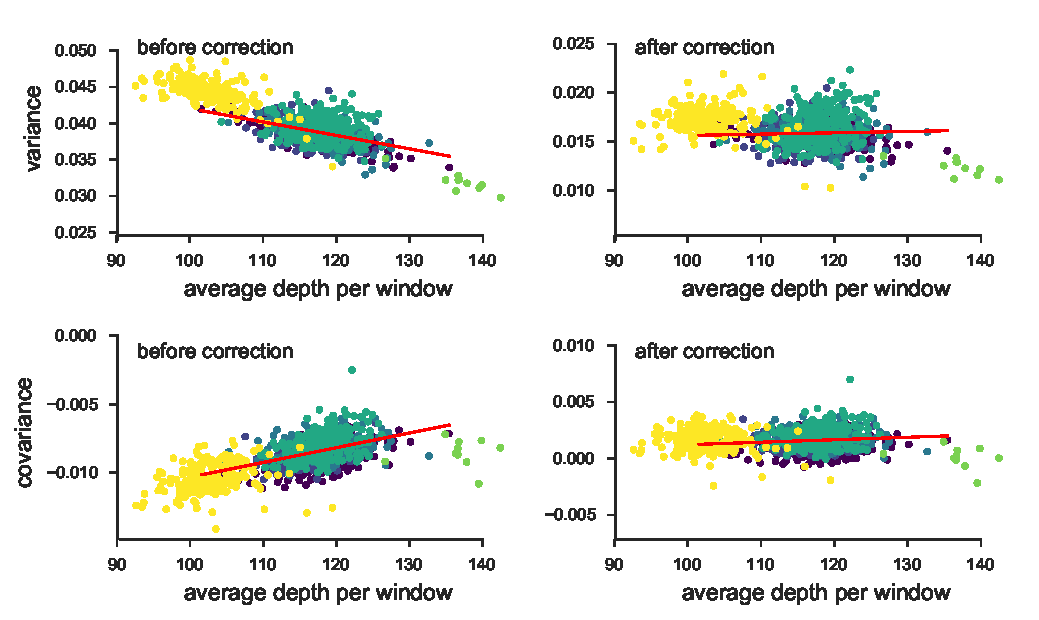
\includegraphics[]{figures/barghi-correction-plot.pdf}

  \caption[Bias correction diagonistic plot for the \textcite{Barghi2019-qy}
  study]{The variance and covariances from the \textcite{Barghi2019-qy} study,
    calculated in 100kb genomic windows plotted against average depth in a
    window before and after bias correction.  Each panel has a least-squares
    estimate between the variance and covariance, and the average depth.
    Overall, the bias correction corrects sampling bias in both the variance
    and covariance such that the relationship with depth is constant. Colors
  indicate the different chromosomes of \emph{D. simulans}; we have excluded
the X chromosome (yellow points) and chromosome 4 points (green points to far
right) from the regression due to large differences in average coverage.}

  \label{suppfig:barghi-correction}
\end{figure}

\clearpage 

\subsection{\textcite{Barghi2019-qy} Binsize Cross-Validation}
\begin{figure}[!ht]
  \centering
  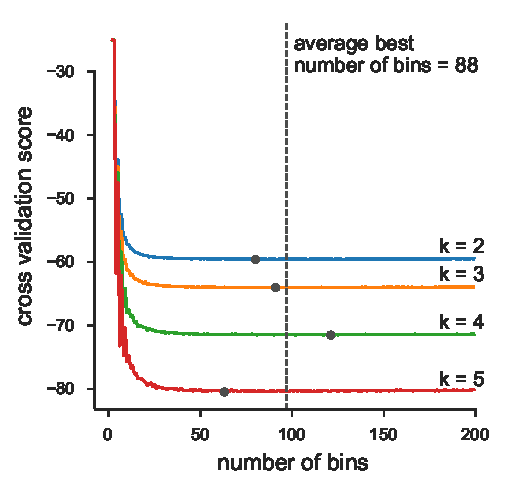
\includegraphics[]{figures/barghi-cross-validation-binsize.pdf}

  \caption[Cross-Validation of binsize]{We chose number of bins used in the histograms of Figure
    \ref{fig:figure-3} via an analytic expression for the cross-validation
    risk, based on the equation 6.16 of (\cite{Wasserman2006-jl}, p. 129).
    Above, we plot the cross-validation risk for various numbers of bins, for
    each of the four off-diagonals of the temporal covariance matrix that we
    analyze. Overall, because the number of data points is large, oversmoothing
    is less of a problem, leading the cross-validation risk to be relatively
    flat across a large number of bins. Each gray point indicates the minimal
    risk for a particular off-diagonal, and the dashed line indicates the best
    average binwidth across off-diagonals.}
  \label{suppfig:barghi-cross-validation-binsize}
\end{figure}


\clearpage 

\subsection{\textcite{Barghi2019-qy} Empirical Null and Windowed Covariance Distributions}
\begin{figure}[!ht]
  \centering
  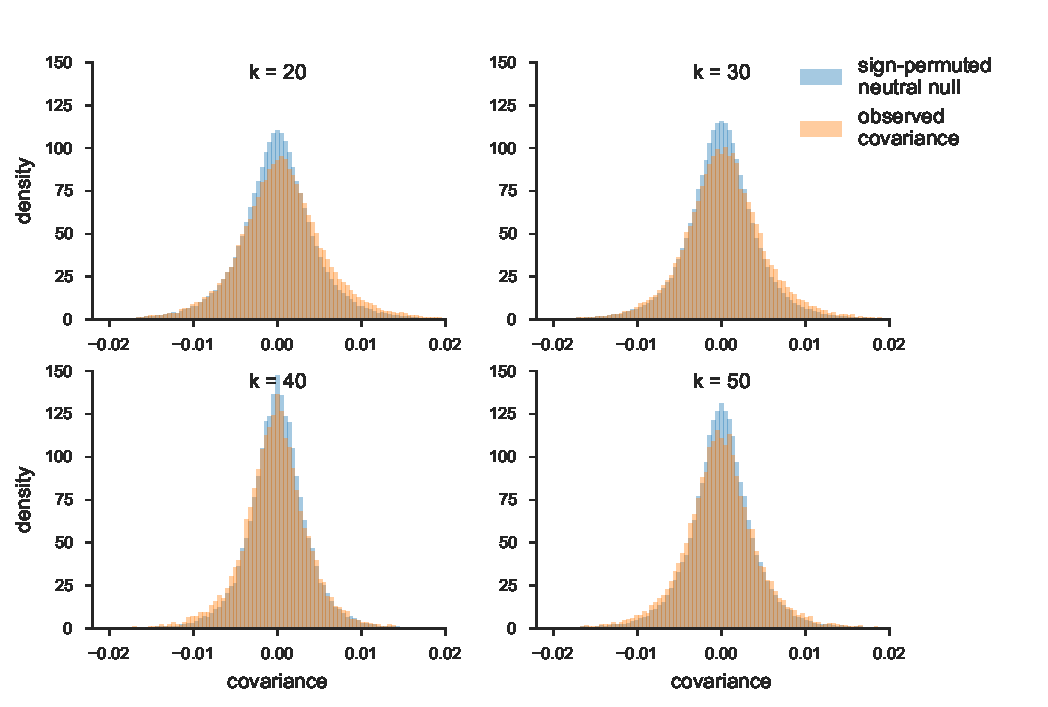
\includegraphics[]{figures/barghi-offset-panels.pdf}

  \caption[Distribution of windowed covariances and empirical null distribution
  for 100kb window size]{The distribution of temporal covariances calculated
    across 100kb genomic windows from \textcite{Barghi2019-qy}'s study (orange)
    and the block sign permuted empirical neutral null distribution of the
  windowed covariances (blue). Each panel shows these windowed covariances and
the empirical null distribution for covariances $\cov(\Delta p_t, \Delta
p_{t+k})$, $k$ is the number of generations between allele frequency changes.}
\label{suppfig:barghi-empnull-tilecovs} \end{figure}


\clearpage 
\begin{figure}[!ht]
  \centering
  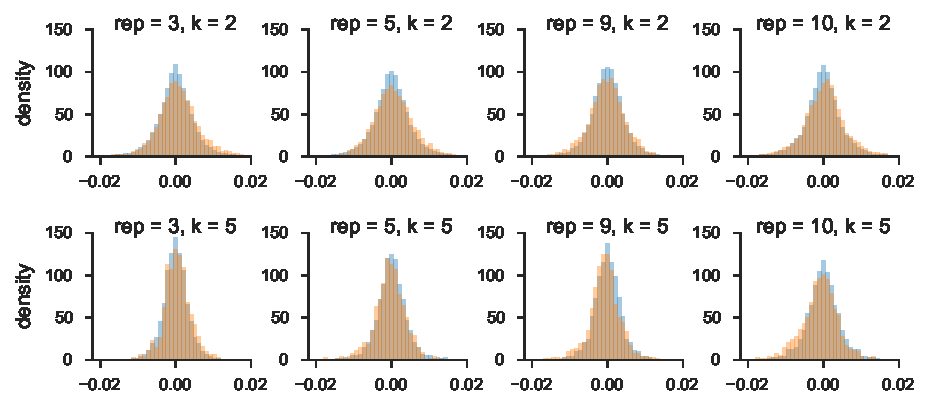
\includegraphics[]{figures/barghi-offset-replicate-panels.pdf}

  \caption[Distributions of windowed covariances and empirical null
  distributions for individual replicates]{The distribution of windowed
    temporal covariances alongside the empirical neutral null for five randomly
    sampled replicates (columns), for $k=2$ (first row) and $k=5$ (second row).
    The main figure of the paper pools all replicate window and empirical
    neutral null covariances; we show here the windowed temporal covariances
    tend to shift from being positive (a heavier right tail) to become more
  negative (a heavier left tail) through time within particular replicates.}
  
  \label{suppfig:barghi-offset-replicate-panels}
\end{figure}


\begin{figure}[!ht]
  \centering
  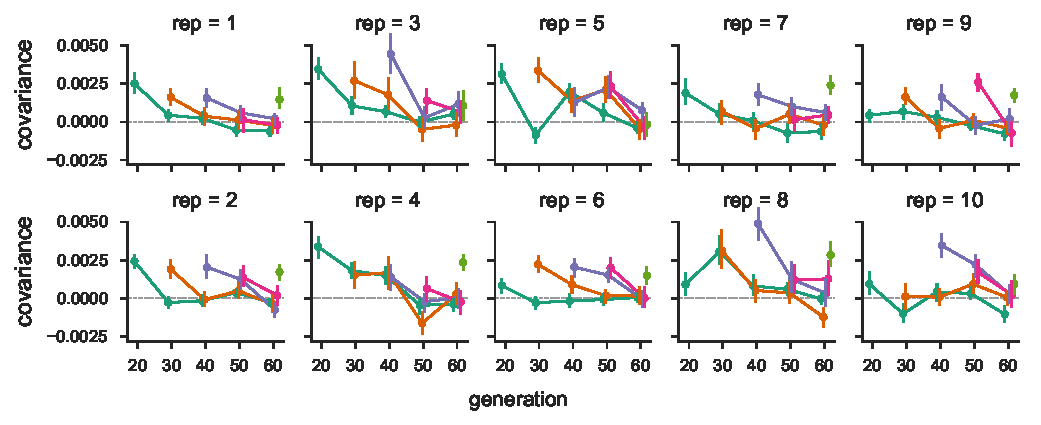
\includegraphics[]{figures/barghi-cov-panels.pdf}

  \caption[Temporal covariances for the \textcite{Barghi2019-qy} study for
  individual replicates]{The temporal covariances from the
    \textcite{Barghi2019-qy} study, for each replicate individually. As in
    Figure \ref{fig:figure-1}, each line follows the temporal covariances from
  some initial reference generation through time, which represent the rows of
temporal covariance matrix.}

  \label{suppfig:barghi-cov-panels}
\end{figure}


\clearpage 

\clearpage 
\subsection{\textcite{Barghi2019-qy} Tail Probabilities for Windowed Covariances Distributions}

\begin{figure}[!ht]
  \centering
  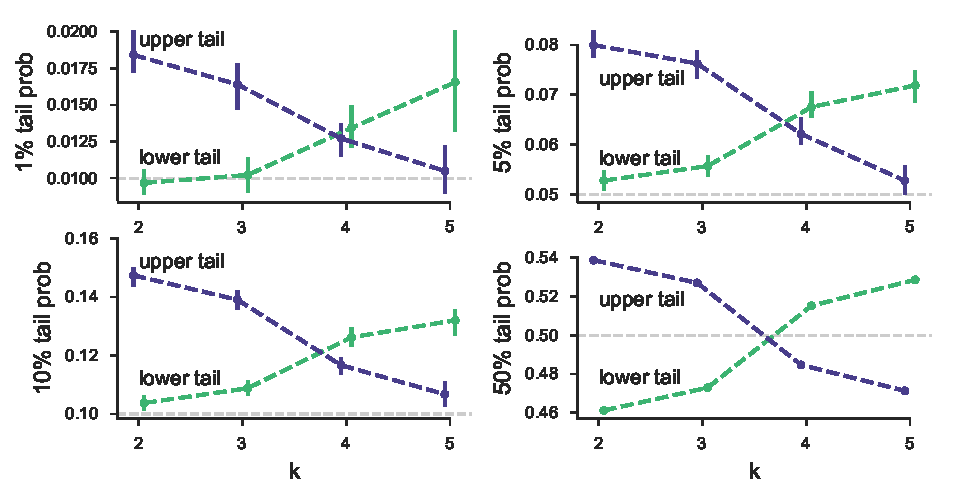
\includegraphics[]{figures/barghi-tailprobs-panels.pdf}

  \caption[]{Tail probabilities of \textcite{Barghi2019-qy} data for various
  $\alpha$ levels}

  \label{suppfig:barghi-tailprobs-panels}
\end{figure}

%\clearpage 
\begin{figure}[!ht]
  \centering

  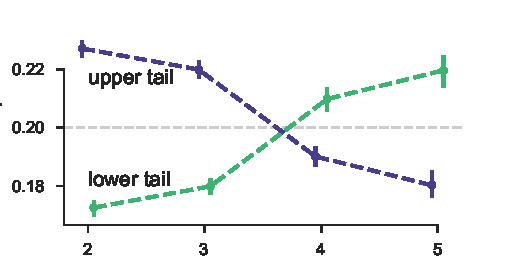
\includegraphics[]{figures/barghi-tailprobs-seqid-20.pdf}

  \caption[20\% tail probabilities based on sign-permuting whole
  chromosomes]{The 20\% lower and upper tail probabilities for the observed
    windowed covariances from the \textcite{Barghi2019-qy} study, based on
    sign-permuting at the chromosome level. This permutation empirical null is
  robust to long-range linkage disequilibrium acting over entire chromosomes.}
  
  \label{suppfig:barghi-tailprobs-seqid}
\end{figure}

\clearpage 

\subsection{\textcite{Bergland2014-ij} Re-Analysis}
\label{bergland-reanlysis}


We also applied our temporal covariance approach to \textcite{Bergland2014-ij},
which found evidence of genome-wide fluctuating selection between Spring and
Fall seasons across three years in \emph{Drosophila melanogaster}. As described in
\textcite{Buffalo2019-io}, we might expect positive covariances between like
seasons changes (i.e. Spring 2010 to Fall 2010 and Spring 2011 to Fall 2011),
and negative covariances between dislike seasonal changes (i.e. Fall 2009 to
Spring 2010 and Fall 2010 to Spring 2011) when fluctuating selection is strong
and acts genome-wide, as the original study found. However, while we find
temporal covariances that are non-zero, we find only weak support for a
seasonal fluctuating model driving these covariances.  In Supplementary Figure
\ref{suppfig:bergland-covs-figure}, we show the temporal covariances from
varying reference generations, across seasonal transitions that are alike (e.g.
the covariance between the allele frequency changes between Fall 2009 and
Spring 2009, and frequency changes between Fall 2010 and Spring 2010), and
dislike (e.g. the covariance between the allele frequency change between Fall
2009 and Spring 2009, and the frequency changes between Spring 2010 and Fall
2009). The first row of temporal covariance matrix is consistent with
fluctuating selection operating for two timepoints, as the first covariance is
negative, and the second is positive, and later covariances are not
statistically differentiable from zero (which could occur if LD and additive
genetic variance decay). However, the all other temporal covariances do not fit
the pattern we would expect under genome-wide fluctuating selection.

\begin{figure}[!ht]
  \centering
  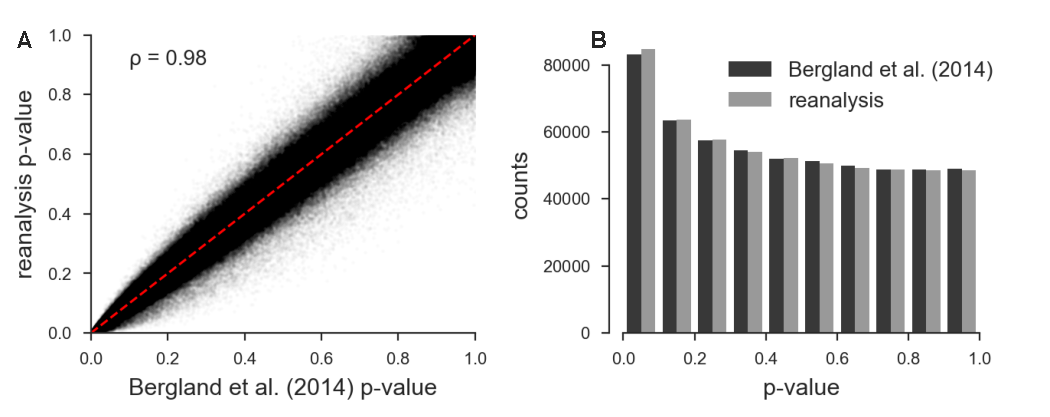
\includegraphics[]{figures/bergland_pvalues.pdf}

  \caption[Scatterplot and distribution of p-values from the original
  \textcite{Bergland2014-ij} study and our reanalysis]{A: Scatterplot of the
    original unadjusted p-values from \textcite{Bergland2014-ij} and the
    p-values from our reanalysis of the same data using the same statistical
    methods; the minor discrepancy is likely due to software version
    differences. B: The histograms of the p-values of our reanalysis and the
    original \textcite{Bergland2014-ij} data; again the minor discrepancy is
  likely due to software differences. Overall, our implementation of Bergland
et al.'s statistical methods produces results very close to the original
analysis.}

  \label{suppfig:bergland-pvalue-comparison}
\end{figure}

We wanted to establish that our temporal-covariance matrix bias correction was
working correctly. We find that it corrects the relationship between depth and
both variance and covariance (Supplementary Figure
\ref{suppfig:bergland-correction}) as expected.

It is unclear how strong the fluctuations would have to be to generate a
genome-wide average signal of fluctuating selection from temporal covariances.
For example, many loci could still show a signal of fluctuating selection, but
the average signal could be overwhelmed by other signals of other selection. To
investigate whether there was an genome-wide excess of loci showing evidence of
fluctuating selection we reanalyzed the data of \parencite{Bergland2014-ij}
using the same seasonal fluctuating model as the original paper. This model is
a Binomial logit-linked GLM fit per-locus, where the Spring/Fall seasons are
encoded as a dummy variable, and are regressed on the frequency data. We use
the same binomial weighting procedure as \textcite{Bergland2014-ij}, where the
weights are determined by the effective number of chromosomes, $N_{eff} = (2
n_t d_t - 1) / (2 n_t + d_t)$ ($n_t$ and $d_t$ are the number of diploid
individuals and the read depth at timepoint $t$, respectively). We fit this
model on all loci marked as used in the VCF provided with the
\textcite{Bergland2014-ij} study (doi:10.5061/dryad.v883p). Overall, our
p-values for the Wald test for each locus closely match those of the original
paper (Pearson correlation coefficient 0.98, p-value < $2.2 \times 10^{-16}$;
see Supplementary Figure \ref{suppfig:bergland-pvalue-comparison} A), and the
histograms of the p-values are nearly identical (Supplementary Figure
\ref{suppfig:bergland-pvalue-comparison} B). \textcite{Bergland2014-ij} find
loci with a significant association with season after a Benjamini and Hochberg
FDR p-value adjustment \parencite{Benjamini1995-jy}, however, the null
hypothesis of the Wald test does not give us an idea of the expected number of
variants that may spuriously fit the pattern of seasonal fluctuating
selection.

% ======= We were concerned that this might be due to a flaw in our methods. To
% address this concern, we first ensured that our temporal-covariance matrix
% bias correction was working as expected. We find that it corrects the
% relationship between depth and both variance and covariance (Supplementary
% Figure \ref{suppfig:bergland-correction}) as expected. We then re-analyzed
% the data of \parencite{Bergland2014-ij} using the same seasonal fluctuating
% model as the original paper. This model is a Binomial logit-linked GLM fit
% per-locus, where the Spring/Fall seasons are encoded as a dummy variable, and
% are regressed on the frequency data. We use the same binomial weighting
% procedure as \textcite{Bergland2014-ij}, where the weights are determined by
% the effective number of chromosomes, $N_{eff} = (2 n_t d_t - 1) / (2 n_t +
% d_t)$ ($n_t$ and $d_t$ are the number of diploid individuals and the read
% depth at timepoint $t$, respectively). We fit this model on all loci marked
% as used in the VCF provided with the \textcite{Bergland2014-ij} study
% (doi:10.5061/dryad.v883p).  Overall, our p-values for the Wald test for each
% locus closely match those of the original paper (Pearson correlation
% coefficient 0.98, p-value < $2.2 \times 10^{-16}$; see Supplementary Figure
% \ref{suppfig:bergland-pvalue-comparison} A), and the histograms of the
% p-values are nearly identical (Supplementary Figure
% \ref{suppfig:bergland-pvalue-comparison} B).  >>>>>>>
% d95c3549a10dc0037f40a54cb8b41f9d412ed1ed

\begin{figure}[!ht]
  \centering
  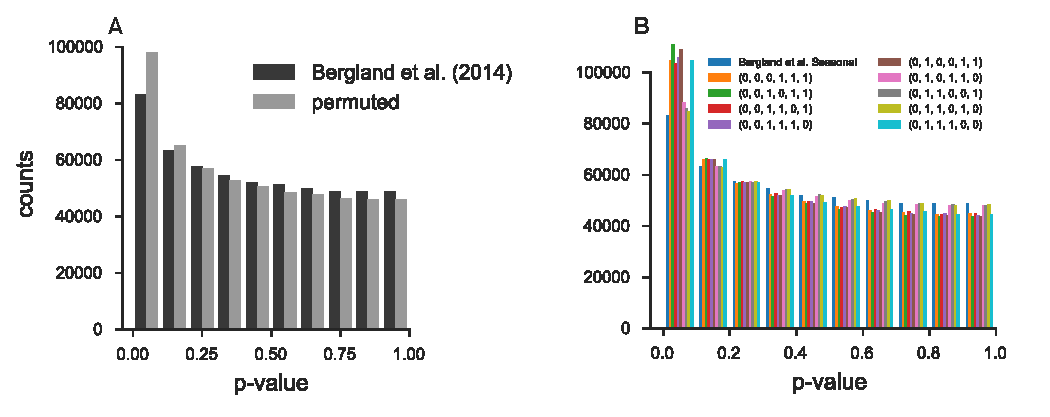
\includegraphics[]{figures/bergland-combined-hists.pdf}

  \caption[Distribution of p-values from the \textcite{Bergland2014-ij} study
  alongside permutation distribution]{Distribution of p-values from the
    \textcite{Bergland2014-ij} study alongside permutation p-values at the loci
    level (A) and for each possible unique permutation (B).}

  \label{suppfig:bergland-pvalue-hist}
\end{figure}


\begin{figure}[!ht]
  \centering
  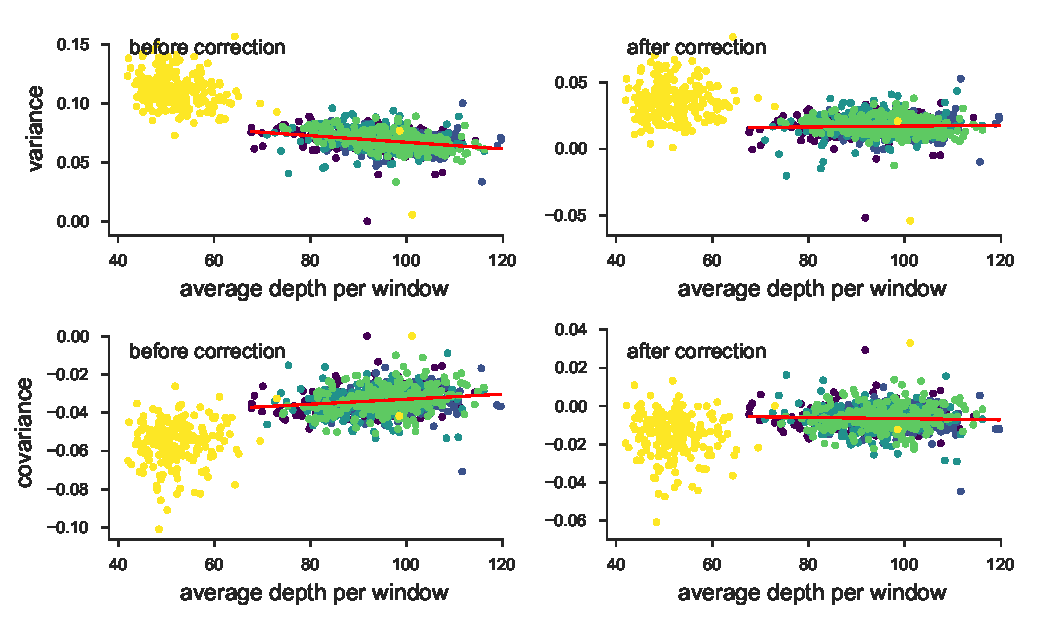
\includegraphics[]{figures/bergland-correction-plot.pdf}

  \caption[Bias correction diagnostic plot for the \textcite{Bergland2014-ij}
  data]{The variance and covariances from the \textcite{Bergland2014-ij} study,
    calculated in 100kb genomic windows plotted against average depth in a
    window before and after bias correction. Each panel has a least-squares
    estimate between the variance and covariance, and the average depth.  The
    bias correction procedure is correcting sampling bias in both the variance
    and covariance such that the relationship with depth is constant. Colors
    indicate the different chromosomes of \emph{D. melanogaster}; we have
    excluded the X chromosome (yellow points; chromosome 4 was not in the
    original study) from the regression due to large differences in average
  coverage.}

  \label{suppfig:bergland-correction}
\end{figure}



To investigate whether there is a genome-wide evidence of an enrichment of
fluctuating selection we created an empirical null distribution by randomly
permuting the season labels and re-running the per-locus seasonal GLM model, as
proposed by \textcite{Machado2018-cs}. We find, regardless of whether we
permute at the locus-level or the permutation replicate-level, that the
observed seasonal p-value distribution \textcite{Bergland2014-ij} is not
enriched for significant p-values beyond what we would expect from the
permutation null. In fact, there appears there is more enrichment for low
p-values when seasonal labels are randomly permuted (Supplementary Figure
\ref{suppfig:bergland-pvalue-hist}, suggesting by random chance we might expect
more variants with a seasonal fluctuating pattern than found in the original
\textcite{Bergland2014-ij} study. While surprising, this could be explained by
the presence of temporal structure across the samples not consistent with
seasonal fluctuating selection. Some fraction of the permutations happen to fit
this structure well, leading to an enrichment of small p-values. This
non-seasonal temporal structure is also evident in our temporal covariances
(Supplementary Figure \ref{suppfig:bergland-covs-figure}), where we see strong
evidence of selection (non-zero temporal covariances), yet the pattern does not
follow that of seasonal fluctuating selection.  

%\gc{ADD MORE HERE} TODO

\begin{figure}[!ht]
  \centering
  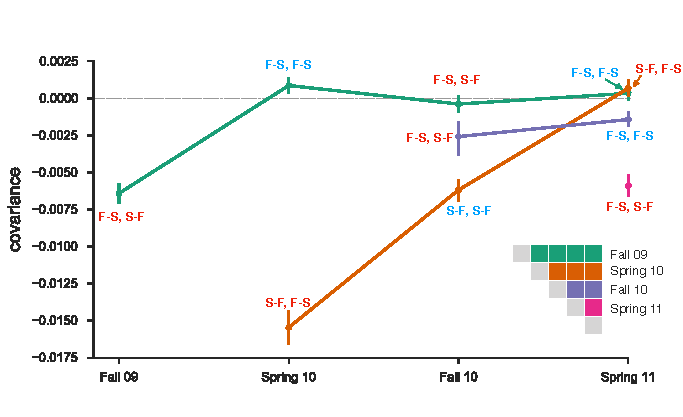
\includegraphics[]{figures/bergland-covs-figure.pdf}

  \caption[Temporal covariances through time for the \textcite{Bergland2014-ij}
  study]{Temporal covariances from the \textcite{Bergland2014-ij} study, from
    varying reference generations (e.g. rows along the temporal covariance
    matrix). Each covariance is labeled indicating whether the covariance is
    between two like seasonal transitions (e.g. the covariance between allele
    frequency changes from fall to spring in one year, and fall to spring in
    another or two dislike seasons (e.g. the covariance between fall to spring
    in one year, and spring to fall in another year). Covariances between like
    transitions are expected to be positive when there is a genome-wide effect
    of fluctuating selection (and these labels are colored blue), while
  covariances between dislike transitions are expected to be negative (and
these labels are colored red). 95\% confidence intervals were constructed by a
block-bootstrapping procedure where the blocks are megabase tiles.}

  \label{suppfig:bergland-covs-figure}
\end{figure}



%\gc{Note that this analysis does not rule out the idea that prior
 % analyses detected {\emph
  %  some} loci showing a pattern of fluctuating selection. Indeed
  %\textcite{Bergland2014-ij} provided a number of analyses that
  %suggested that their loci might be enriched for {\bf XXX}. However,
  %this reanalysis suggests that we currently lack genome-wide evidence
%of many loci experiencing fluctuating selection in {\it in Drosophila
 % melanogaster}. }




\begingroup
\setstretch{0.8}
\setlength\bibitemsep{0pt}

% citations from chapter 1
\nocite{kram2015}
\nocite{dplyr}
\nocite{ggplot2}
\nocite{R}
\nocite{Rossum:1995:PRM:869369}
\nocite{C}
\nocite{colorspace}
\nocite{purrr}
\nocite{tidyr}


\printbibliography
\endgroup


% The UMI abstract uses square brackets!
% \UMIabstract[The UMI abstract is submitted online as plain text. It no longer has a word limit or specific formatting. Therefore, the UMIabstract command is now deprecated.]

\end{document} 
